% Gelfand seminar notes, 1982-83: source pages P001026-P001115.
% English translation (AI-made, checked against the scans), cut page by page from the cumulative working reader A4-reader-chapters01-34-complete-first1527-separated-diplomatic-r53.
% \SourcePage{GELFAND-Pnnnnnn}{label} starts a scanned page; the second argument is the number written
% on the page, if any. Editorial notes give the page, a label and the transcriber's remark; \Unclear
% marks a doubtful reading.
\SourcePage{GELFAND-P001026}{unlabelled}
\underline{6/$\overline{\underline{\mathrm{IX}}}$/82}\qquad
\underline{Gelfand seminar.}

\hfill (40th year of activity)

\underline{Kirillov on the work of Lepowsky and Wilson.}
\[
\begin{array}{rlll}
&(\text{Lepowsky},&\text{Wilson}&\\
\text{generaliz.}&\text{---''---},&\text{---''---},&\text{Kac, Kazdan})
\end{array}
\]

Lie algebra with six generators.
\[
\begin{array}{ccc|l}
e_0&h_0&f_0&\forall\ \text{triple satisfies the standard relations}\\
e_1&h_1&f_1&\text{of matrices of order two with trace }0.
\end{array}
\]


\Needspace{7\baselineskip}
\begin{GelfandAdjacentEvidence}{GELFAND-P001027}{1}
\SourcePage{GELFAND-P001027}{unlabelled}
\underline{\underline{I. M. G.}}\quad \uwave{Cartan algebras}\quad No need to learn the roots (everything follows from this)

$e_i,h_i,f_i,\quad i=1,\ldots,n$

\begin{equation*}
\left\{\begin{aligned}
[e_i,f_k]&=h_i\delta_{ik}\\
[h_i,f_k]&=-a_{ik}f_k\qquad\text{(without summing over $k$)}\\
[h_i,e_k]&=a_{ik}e_k\\
[h_i,h_k]&=0
\end{aligned}\right.
\tag{1}
\end{equation*}
$(a_{ik})$ --- \uwave{Cartan matrix}

$a_{ii}$ can be adjusted by normalizing $f_i$

\underline{Assume}: $a_{ii}=2$.

Important algebras: 1) $a_{ij}<0$ for $i\ne j$

\hspace{4em}2) $a_{ij}\in\mathbb Z$
\SourceFigure{GELFAND-P001027}{strict-offdiagonal}{The manuscript has a strict inequality $<$.}
\end{GelfandAdjacentEvidence}
\begin{GelfandAdjacentEvidence}{GELFAND-P001027}{2}


As a rule there are no further relations (so that no linear combination of $e_i,h_i,f_i$ is forced to be $0$)

Sometimes one can add relations, and the theorem is that \underline{they are unique.}

\begin{equation*}
\left\{\begin{aligned}
e_i^{-a_{ik}+1}e_k&=0\\
f_i^{-a_{ik}+1}f_k&=0
\end{aligned}\right.
\tag{2}
\end{equation*}
\SourceFigure{GELFAND-P001027}{serre-powers}{The powers of $e_i$ and $f_i$ in (2) are written without the notation $\operatorname{ad}$.}
\end{GelfandAdjacentEvidence}
\begin{GelfandAdjacentEvidence}{GELFAND-P001027}{3}


Sometimes the algebra is finite-dimensional,

\underline{$n=1$}: \quad $e_1,f_1,h_1$
\[
\begin{aligned}
[e_1,f_1]&=h_1\\
[h_1,e_1]&=2e_1\\
[h_1,f_1]&=-2f_1
\end{aligned}
\]
\SourceFigure{GELFAND-P001027}{sl2-last-index}{The last subscript in $-2f_1$ has the foot of the numeral $1$.}
\end{GelfandAdjacentEvidence}
\begin{GelfandAdjacentEvidence}{GELFAND-P001027}{4}


this gives $\mathrm{sl}(2)$
\Unclear{GELFAND-P001027}{cancel-after-sl2}{A short entry after $\mathrm{sl}(2)$ is heavily crossed out.}
\end{GelfandAdjacentEvidence}


Finite-dimensionality $\Leftrightarrow$ the matrix $(a_{ij})>0$ (strictly)

Affine $\Leftrightarrow$ $(a_{ij})\ge0$ and $\operatorname{rank}(a_{ij})=n-1$.

\underline{$n=2$}
\[
\begin{array}{ccc}
\begin{pmatrix}2&-1\\-1&2\end{pmatrix}&
\begin{pmatrix}2&-1\\-2&2\end{pmatrix}&
\begin{pmatrix}2&-1\\-3&2\end{pmatrix}\\
\mathrm{sl}(3)&\mathrm{so}(5)&G_2
\end{array}
\]

This replaces Dynkin diagrams.

Relations (2) for $\mathrm{sl}(3)$:
\begin{align*}
[e_1[e_1e_2]]&=0\\
[e_2[e_2e_1]]&=0
\end{align*}


\Needspace{7\baselineskip}
\begin{GelfandAdjacentEvidence}{GELFAND-P001028}{1}
\SourcePage{GELFAND-P001028}{4}
\underline{Affine algebras}:
\[
\begin{pmatrix}2&-2\\-2&-2\end{pmatrix}\qquad A_1^1
\]
\SourceFigure{GELFAND-P001028}{affine-lower-right}{The lower-right entry of the first matrix is written as $-2$.}
\end{GelfandAdjacentEvidence}
\begin{GelfandAdjacentEvidence}{GELFAND-P001028}{2}

\[
\begin{pmatrix}2&-4\\-1&2\end{pmatrix}
\]
\Unclear{GELFAND-P001028}{cancel-affine-label}{An entry to the right of the second matrix is crossed out.}
\end{GelfandAdjacentEvidence}
\begin{GelfandAdjacentEvidence}{GELFAND-P001028}{3}


\underline{Heisenberg algebra}:
\[
\underset{\substack{\vert\\\text{symplectic}}}{E}\oplus R,\qquad
[x,y]=\langle x,y\rangle 1,\quad 1\in R,
\]
$\langle x,y\rangle$ --- symplectic product.

\begin{center}--- $\cdot$ ---\end{center}

\underline{Kirillov.}
\[
\begin{pmatrix}2&-2\\-2&2\end{pmatrix}\qquad
\begin{array}{ccc}f_1&h_1&e_1\\f_2&h_2&e_2\end{array}
\]
Nontrivial relation
\[
[e_1[e_1[e_1,e_2]]]=0
\]
and analogous relations with the replacements \(\begin{array}{c}1\leftrightarrow2\\e\leftrightarrow f\end{array}\).

\underline{I. M. G.} \uwave{Root vectors} --- monomials;
\Unclear{GELFAND-P001028}{cancel-root-word}{An entry before “monomials” is crossed out.}
\end{GelfandAdjacentEvidence}
\begin{GelfandAdjacentEvidence}{GELFAND-P001028}{4}


weights are the numbers of occurrences of $e_j$
\Unclear{GELFAND-P001028}{cancel-weight-word}{The first strokes of the crossed-out word may begin «вхо…», as in “occurrences”.}
\end{GelfandAdjacentEvidence}
\begin{GelfandAdjacentEvidence}{GELFAND-P001028}{5}


\underline{K.}

Grading: weights (pairs of numbers)
\Unclear{GELFAND-P001028}{cancel-grading}{An entry after “Grading” is crossed out.}
\end{GelfandAdjacentEvidence}
\begin{GelfandAdjacentEvidence}{GELFAND-P001028}{6}


\SourceFigure{GELFAND-P001028}{root-diagram}{%
\begingroup\color{black}\GelfandFitDiagram{\begin{tikzpicture}[x=.83cm,y=.71cm,line width=.47pt,
every node/.style={inner sep=1pt,font=\scriptsize}]
\draw (-1.52,0)--(1.95,.04);
\draw (0,1.53)--(0,-1.15);
\node[draw,ellipse] at (-1.51,0) {$f_1$};
\node[draw,ellipse] at (0,0) {$h_1\ h_2$};
\node[draw,ellipse] at (1.55,.02) {$e_1$};
\node[draw,ellipse] at (.08,-1.15) {$f_2$};
\node[draw,ellipse] (top) at (.13,1.45) {$e_2$};
\node[draw,ellipse] (comm) at (1.89,1.41) {$[e_1,e_2]$};
\node[draw,ellipse] (second) at (4.02,1.48) {$[[e_2e_1]e_1]$};
\node[draw,ellipse] (above) at (1.87,2.38) {$[e_1,e_2]e_2$};
\node (zero) at (5.92,1.48) {$0$};
\draw (top.east)--(comm.west);
\draw (comm.east)--(second.west);
\draw[->] (second.east)--(zero.west);
\draw (1.62,.28)--(1.71,.96);
\draw (comm.north)--(above.south);
\end{tikzpicture}}\endgroup\par
The upper oval reads $[e_1,e_2]e_2$. Any outer brackets remain uncertain.}
\end{GelfandAdjacentEvidence}
\begin{GelfandAdjacentEvidence}{GELFAND-P001028}{7}


\underline{I. M. G.}
\SourceFigure{GELFAND-P001028}{monomial-path}{%
\begingroup\color{black}\GelfandFitDiagram{\begin{tikzpicture}[x=1cm,y=1cm]
\draw (0,0)--(.03,1.05)--(.60,1.05)--(.57,1.65)--(1.16,1.65);
\fill (0,0) circle[radius=1.25pt];
\fill (.02,.50) circle[radius=1.05pt];
\end{tikzpicture}}\endgroup}
\end{GelfandAdjacentEvidence}
\begin{GelfandAdjacentEvidence}{GELFAND-P001028}{8}

\uwave{monomials}: paths like $e_1e_1e_2e_1\ldots$

\underline{Question}: how can the paths be made continuous?

\underline{K.} \uwave{Second realization.} Functions on the circle with values in matrices of order two.

$A(t)$ (polynomials in $t$ and $t^{-1}$; defined for $|t|=1$).

\begin{equation*}
[A,B]=AB-BA+\frac{\mathbf1}{2\pi i}\int\operatorname{tr}(A\,dB),
\qquad\mathbf1\text{ --- a new generator}
\tag{1}
\end{equation*}

\Unclear{GELFAND-P001028}{cancel-above-e1}{An entry above $e_1$ is crossed out.}
\end{GelfandAdjacentEvidence}
\begin{GelfandAdjacentEvidence}{GELFAND-P001028}{9}

\begin{equation*}
\begin{aligned}
e_1&=\begin{pmatrix}0&1\\0&0\end{pmatrix},&
h_1&=\begin{pmatrix}1&0\\0&-1\end{pmatrix},&
f_1&=\begin{pmatrix}0&0\\1&0\end{pmatrix}\\
e_2&=\begin{pmatrix}0&0\\t&0\end{pmatrix},&
h_2&=\begin{pmatrix}-1&0\\0&1\end{pmatrix}+\mathbf1&
f_2&=\begin{pmatrix}0&t^{-1}\\0&0\end{pmatrix}
\end{aligned}
\tag{2}
\end{equation*}
\Unclear{GELFAND-P001028}{cancel-after-h1}{The entry between the matrix for $h_1$ and the comma is heavily crossed out.}
\end{GelfandAdjacentEvidence}
\begin{GelfandAdjacentEvidence}{GELFAND-P001028}{10}

\SourceFigure{GELFAND-P001028}{central-entry}{The matrix for $h_2$ in (2) is followed by $+\mathbf1$.}
\end{GelfandAdjacentEvidence}
\begin{GelfandAdjacentEvidence}{GELFAND-P001028}{11}


They satisfy all the relations.
\Unclear{GELFAND-P001028}{cancel-before-they}{An entry at the beginning of the line before “They” is crossed out.}
\end{GelfandAdjacentEvidence}
\begin{GelfandAdjacentEvidence}{GELFAND-P001028}{12}


\underline{I. M. G.} Pick out the Heisenberg subalgebra, the type of its representations, etc.
\Unclear{GELFAND-P001028}{heisenberg-verb}{The word before “its representations” most likely reads “type”.}
\end{GelfandAdjacentEvidence}
\begin{GelfandAdjacentEvidence}{GELFAND-P001028}{13}


\underline{K.} This is convenient for writing a general element.
\begin{equation*}
\begin{pmatrix}a(t)&e(t)\\c(t)&-a(t)\end{pmatrix}+\alpha\mathbf1.
\tag{3}
\end{equation*}
\Unclear{GELFAND-P001028}{generic-matrix-entry}{The upper-right letter resembles $e$, with a short loop. A reading of $b$ remains possible.}
\end{GelfandAdjacentEvidence}



\Needspace{7\baselineskip}
\begin{GelfandAdjacentEvidence}{GELFAND-P001029}{1}
\SourcePage{GELFAND-P001029}{unlabelled}
There are many representations; they have not all been described (and pointless) [tentative reading of the abbreviation]\textsuperscript{?}
\Unclear{GELFAND-P001029}{opening-parenthesis}{(and pointless) [tentative reading of the abbreviation]}
\end{GelfandAdjacentEvidence}
\begin{GelfandAdjacentEvidence}{GELFAND-P001029}{2}


The highest-weight representations are described.

One of them is singled out and is remarkable:

cyclic vector --- highest-weight vector $v_0$
\begin{equation*}
\left\{\begin{aligned}
e_1v_0&=0,\\
e_2v_0&=0,\\
h_1v_0&=0,\\
h_2v_0&=v_0
\end{aligned}\right.
\tag{4}
\end{equation*}

The most economical highest-weight representation

The space is realized as the space of [Crossed out: illegible.]\textsuperscript{?}
\Unclear{GELFAND-P001029}{cancel-before-polynomials}{[Crossed out: illegible.]}
\end{GelfandAdjacentEvidence}
\begin{GelfandAdjacentEvidence}{GELFAND-P001029}{3}

polynomials in $x_1,x_3,x_5,\ldots,x_{2n+1},\ldots$
\SourceFigure{GELFAND-P001029}{first-polynomial-index}{The first indices in the list: \(1,3,5\).}
\end{GelfandAdjacentEvidence}
\begin{GelfandAdjacentEvidence}{GELFAND-P001029}{4}


A Heisenberg (infinite-dimensional) subalgebra is singled out:
\begin{equation*}
B_{2k+1}=\begin{pmatrix}0&t^k\\t^{k+1}&0\end{pmatrix},\quad
C_{2k+1}=\begin{pmatrix}0&-t^k\\t^{k+1}&0\end{pmatrix},\quad
H_{2k}=\begin{pmatrix}t^k&0\\0&-t^k\end{pmatrix}.
\tag{5}
\end{equation*}

\begin{center}--- $\cdot$ ---\end{center}

\underline{I. M. G.}: This algebra arises naturally in the \(p\)-adic case.

Consider the case in which we quotient by $\{\mathbf1\}$

\underline{K.} There are different (nonconjugate) commutative subalgebras.

1) diagonal

2) $\begin{pmatrix}0&f(t)\\tf(t)&0\end{pmatrix}$

One cannot put it in diagonal form continuously (but one can for each fixed value).

\underline{I. M. G.} \uwave{Quadratic forms}: a related problem; \quad Mishchenko; Gelfand --- the number is $2^n$,

\hspace{5em}but the canonical forms are undescribed.

\underline{K.} with \(\mathbf1\) these algebras are now noncommutative
\[
[B_{2k+1},B_{2\ell+1}]=\delta(k+\ell)(2\ell+1)\mathbf1
\]
\SourceFigure{GELFAND-P001029}{heisenberg-delta}{The manuscript reads \(\delta(k+\ell)(2\ell+1)\mathbf1\).}
\end{GelfandAdjacentEvidence}
\begin{GelfandAdjacentEvidence}{GELFAND-P001029}{5}


(Heisenberg algebra)

Take its standard representation.
\[
\begin{array}{ll||l}
B_1,B_3,\ldots & \text{--- multiplication by }x_1,x_2,\ldots & B_k=x_k(2k+1)\\
B_{-1},B_{-3},\ldots & \text{--- differentiation} & B_{-k}=\partial/\partial x_k
\end{array}
\]
\SourceFigure{GELFAND-P001029}{heisenberg-action-indices}{The notation in the two manuscript columns.}
\end{GelfandAdjacentEvidence}
\begin{GelfandAdjacentEvidence}{GELFAND-P001029}{6}


The restriction of the representation to the Heisenberg algebra remains irreducible.

Generating function for the action
\[
e^{\sum x_k}e^{4\sum\partial/\partial x_k}\overset{df}{=}L=\sum L_m,
\qquad L_m\text{ --- homogeneous component of weight }m.
\]
\SourceFigure{GELFAND-P001029}{generator-exponents}{The two exponential arguments in the manuscript.}
\end{GelfandAdjacentEvidence}
\begin{GelfandAdjacentEvidence}{GELFAND-P001029}{7}


$\bigl(\forall x_k\text{ has }\underset{\substack{\downarrow\\(-k)}}{\text{its own weight}}\bigr)$
\Unclear{GELFAND-P001029}{final-parenthesis}{(not written out) [tentative reading]}
\end{GelfandAdjacentEvidence}
\begin{GelfandAdjacentEvidence}{GELFAND-P001029}{8}

\SourceFigure{GELFAND-P001029}{weight-arrow}{Arrow labelled \((-k)\) below “weight”.}
\end{GelfandAdjacentEvidence}


$C_{2k+1}$ and $H_{2k}$ are expressed by simple formulas in terms of $L_m$.


\Needspace{7\baselineskip}
\begin{GelfandAdjacentEvidence}{GELFAND-P001030}{1}
\SourcePage{GELFAND-P001030}{5}
\uuline{Zamolodchikov} (Sasha).

\uuline{On the string}.

It arises from the theory of strong interactions (we neglect something).

There is a mechanical system with coordinates $x^\mu(\sigma)$, $\mu=0,1,\ldots,D-1$.
$\sigma$ --- a continuous index; $\sigma\in(0,2\pi)$ (a circle).
\[
\begin{gathered}
\dot{x}^{\mu}(\sigma)=\frac{\partial}{\partial\tau}x^\mu(\sigma)
\qquad\text{(generalized velocities)},\\[.5ex]
\dot{x}^{\mu}(\sigma,\tau)=\frac{\partial}{\partial\tau}x^\mu(\sigma,\tau)
\end{gathered}
\]

$x^\mu(\sigma,\tau)$\qquad The trajectory is a surface (two-dimensional).
\SourceFigure{GELFAND-P001030}{surface-abbreviation}{The manuscript abbreviation for “two-dimensional.”}
\end{GelfandAdjacentEvidence}
\begin{GelfandAdjacentEvidence}{GELFAND-P001030}{2}


Action:
\begin{equation*}
A[x^\mu]=\int d\tau\int d\sigma\,
\mathcal{L}(x^\mu(\sigma,\tau),\dot{x}^\mu(\sigma,\tau))
\tag{1}
\end{equation*}

$x^\mu$ is regarded as a vector in a space with metric
\[
\operatorname{diag}\bigl(\underset{x^0}{1},\underset{x^1}{-1},
\underset{\ldots}{\ldots},\underset{x^{D-1}}{-1}\bigr)
\]

Choose area as the action:
\begin{equation*}
A[x^\mu]=\int d\sigma\,d\tau
\sqrt{(\dot{x}_\mu)^2(x'_\nu)^2-(\dot{x}_\mu x'^{\mu})^2}
\tag{2}
\end{equation*}
\SourceFigure{GELFAND-P001030}{area-sign}{The expression under the square root in (2).}
\end{GelfandAdjacentEvidence}
\begin{GelfandAdjacentEvidence}{GELFAND-P001030}{3}


Here $x'_\mu=\dfrac{\partial}{\partial\sigma}x_\mu(\sigma,\tau)$.

\begin{equation*}
\text{\uwave{Invariance}:}\qquad
\begin{aligned}
\sigma&\longrightarrow f(\sigma,\tau)\\
\tau&\longrightarrow g(\sigma,\tau)
\end{aligned}
\quad\bigg/\!\bigg/\quad
\begin{gathered}\text{area}\\\text{is unchanged}\end{gathered}
\tag{3}
\end{equation*}

This is a relativistically invariant model.

Mass is proportional to length; a point interacts with its nearest neighbors.
As it contracts, it reaches relativistic speeds.

Momenta:
\begin{equation*}
p_\mu(s)=\frac{\partial\mathcal{L}}{\partial\dot{x}_\mu(\sigma)}
\tag{4}
\end{equation*}
\SourceFigure{GELFAND-P001030}{momentum-argument}{The left side uses \(s\) and the right side uses \(\sigma\).}
\end{GelfandAdjacentEvidence}
\begin{GelfandAdjacentEvidence}{GELFAND-P001030}{4}


The Lagrangian is degenerate $\Rightarrow$ (4) cannot be solved for the velocities; there are relations between coordinates and momenta:
\begin{equation*}
\begin{cases}
M(\sigma)=(p_\mu(\sigma))^2-(x'_\mu(\sigma))^2=0\\
K(\sigma)=x'_\mu(\sigma)p^\mu(\sigma)=0
\end{cases}
\qquad\text{(constraints)}
\tag{5}
\end{equation*}
\SourceFigure{GELFAND-P001030}{constraint-minus}{The minus sign in the first constraint.}
\end{GelfandAdjacentEvidence}


\begin{equation*}
H=\sum p\dot{x}-L\qquad\Rightarrow\qquad H\equiv0
\tag{6}
\end{equation*}

\underline{Worked on by}: Barbashov, Chernikov (classical theory);
Nambu --- connections with dual models.

$(5),(6)\Rightarrow$ one must use Dirac's formalism (see Dirac's book).


\Needspace{7\baselineskip}
\begin{GelfandAdjacentEvidence}{GELFAND-P001031}{1}
\SourcePage{GELFAND-P001031}{unlabelled}
\begin{equation*}
L^{(\pm)}(\sigma)=(p_\mu\pm x'_\mu)^2=0
\tag{7}
\end{equation*}
\Unclear{GELFAND-P001031}{cancelled-l-subscript}{The cancelled subscript under \(L^{(\pm)}\) is illegible.}
\end{GelfandAdjacentEvidence}
\begin{GelfandAdjacentEvidence}{GELFAND-P001031}{2}

\SourceFigure{GELFAND-P001031}{square-constraints}{The square in (7).}
\end{GelfandAdjacentEvidence}
\begin{GelfandAdjacentEvidence}{GELFAND-P001031}{3}


Standard commutation relations defining the Poisson bracket:
\begin{equation*}
\{p_\mu(\sigma),x^\nu(\sigma')\}=\delta^\nu_\mu\delta(\sigma-\sigma')
\tag{8}
\end{equation*}

Consider the Fourier expansion of $x^\nu$ and $p_\mu$:
\begin{equation*}
\begin{cases}
x_\mu(\sigma)=\displaystyle\sum_{n=-\infty}^{\infty}e^{in\sigma}x_\mu^{(n)}\\[.5ex]
p_\mu(\sigma)=\displaystyle\sum e^{-in\sigma}p_\mu^{(n)}
\end{cases}
\tag{9}
\end{equation*}
\Unclear{GELFAND-P001031}{cancelled-fourier-right}{Illegible cancelled entry to the right of the second line of (9).}
\end{GelfandAdjacentEvidence}
\begin{GelfandAdjacentEvidence}{GELFAND-P001031}{4}


Then
\begin{equation*}
\{p^\mu_n,x_{m\nu}\}=\delta^\mu_\nu\delta_{0,n+m}.
\tag{10}
\end{equation*}
\SourceFigure{GELFAND-P001031}{fourier-bracket-indices}{The exponents \(in\sigma,-in\sigma\) and the index \(0,n+m\).}
\end{GelfandAdjacentEvidence}
\begin{GelfandAdjacentEvidence}{GELFAND-P001031}{5}


Expand $L^{(\pm)}(\sigma)$ from (7):
\begin{equation*}
L^{(\pm)}(\sigma)=\sum L_n^{(\pm)}e^{in\sigma}
\tag{11}
\end{equation*}

One can show:
\begin{equation*}
\{L_n^{(+)},L_m^{(-)}\}=0,\qquad
\{L_n^{(+)},L_m^{(+)}\}=(n-m)L_{n+m}^{(+)},\qquad n,m\in\mathbb Z,
\tag{12}
\end{equation*}
(and the same upon replacing $+$ by $-$)

i.e. we obtain the algebra of vector fields on the circle.

\begin{equation*}
\dot{p}_\mu=\{p_\mu,\widetilde H\},\qquad
\dot{x}_\mu=\{x_\mu,\widetilde H\}
\tag{13}
\end{equation*}
\SourceFigure{GELFAND-P001031}{inter-equation-strokes}{$\vert\quad\vert$}
\end{GelfandAdjacentEvidence}
\begin{GelfandAdjacentEvidence}{GELFAND-P001031}{6}


\begin{equation*}
\widetilde H=\alpha_+(\sigma)L^{(+)}+\alpha_-(\sigma)L^{(-)}
\tag{14}
\end{equation*}

Changing $\alpha_\pm(\sigma)$ corresponds to gauge transformations. One can take
\begin{equation*}
\widetilde H=\alpha_+(\sigma,\tau)L^{(+)}+\alpha_-(\sigma,\tau)L^{(-)}
\tag{14'}
\end{equation*}

We must solve the equations (13) with initial data $p_\mu(\sigma,0)$, $x_\mu(\sigma,0)$,
satisfying the condition:
\begin{equation*}
L^{(\pm)}(p(\sigma,0),x(\sigma,0))=0
\tag{15}
\end{equation*}
($\Rightarrow$ they will remain satisfied)

\uwave{Quantize}. We obtain
\begin{equation*}
[p^\mu_n,x_{m\nu}]=i\delta^\mu_\nu\delta_{0,n+m},\qquad
p^\mu_n,x_{m\nu}\text{ --- Hermitian operators}.
\tag{16}
\end{equation*}

A representation of these relations --- ?

Introduce the operators
\begin{equation*}
a_n^\mu=p_n^\mu+i x_{+n}^\mu,\qquad a_{-n}=a_n^+.
\tag{17}
\end{equation*}
\SourceFigure{GELFAND-P001031}{oscillator-x-subscript}{The subscript \(+n\) on \(x\) in (17).}
\end{GelfandAdjacentEvidence}
\begin{GelfandAdjacentEvidence}{GELFAND-P001031}{7}


\begin{equation*}
[a_n^\mu,a_n^{+\nu}]=\delta_{n,m}\delta_{\mu\nu},\qquad n,m\geq0.
\tag{18}
\end{equation*}
\SourceFigure{GELFAND-P001031}{second-oscillator-index}{Both operators on the left carry \(n\). The right side has \(\delta_{n,m}\).}
\end{GelfandAdjacentEvidence}


(the others commute).


\Needspace{7\baselineskip}
\begin{GelfandAdjacentEvidence}{GELFAND-P001032}{1}
\SourcePage{GELFAND-P001032}{6}
\dashuline{Fock representation}:
\begin{equation*}
a_n|0\rangle=0,\quad\forall n\geq0.
\tag{19}
\end{equation*}

$|0\rangle$ --- the vector called the vacuum state.

All the other states should be obtained by acting with $a_n^+$ on $|0\rangle$.
\begin{equation*}
[L_n^{(+)},L_m^{(+)}]=(n-m)L_{n+m}^{(+)}
+\frac{D}{12}(n^3-n)\delta_{0,n+m},
\tag{20}
\end{equation*}
where
\begin{equation*}
L_n^{(+)}=\sum_{k=-\infty}^{\infty}a_k a_{n-k}
\tag{21}
\end{equation*}
(constraint operators)
\Unclear{GELFAND-P001032}{cancelled-before-operators}{Illegible cancelled entry before “constraint operators.”}
\end{GelfandAdjacentEvidence}
\begin{GelfandAdjacentEvidence}{GELFAND-P001032}{2}


(22) \underline{Problem (quantum)}: find a state $\varphi$,
such that $L_n^{(\pm)}|\varphi\rangle=0$.

States of the system (stationary):
\begin{equation*}
\begin{cases}
H(p,q)|\varphi\rangle=E|\varphi\rangle\\
L^i(p,q)|\varphi\rangle=0
\end{cases}
\tag{23}
\end{equation*}

In (20) one must normal-order, with $a_n^+$ to the left of $a_n$.
\SourceFigure{GELFAND-P001032}{normal-order-insertion}{“We have:” is written under the start of the line.}
\end{GelfandAdjacentEvidence}
\begin{GelfandAdjacentEvidence}{GELFAND-P001032}{3}


We have: $L_n^{(+)}|0\rangle=0$, $n\geq0$, but for $n<0$
this fails, and there is no state $|\varphi\rangle$, annihilated by all the $L_n^{(+)}$
(because of the last term in (20)).

\Unclear{GELFAND-P001032}{cancelled-before-result}{The crossed-out word appears to read “Idea.”}
\end{GelfandAdjacentEvidence}
\begin{GelfandAdjacentEvidence}{GELFAND-P001032}{4}

The result is that we satisfy $1/2$ of all the constraints, and that suffices since the \uwave{matrix elements between all physical states} will vanish.

(but only because there is no better option)

In the string problem there are $\infty$ operators commuting with all the constraints. These are the only ones that need quantizing! They have the form:
\begin{equation*}
\begin{gathered}
Q_{\mu_1\ldots\mu_n}^{(n)}=
\int_0^{2\pi}d\sigma_n\int d\sigma_1\,d\sigma_2\ldots d\sigma_{n-1}
\,y_{\mu_1}(\sigma_1)\ldots y_{\mu_n}(\sigma_n)\\
\sigma_n<\sigma_1<\sigma_2<\ldots<\sigma_n+2\pi
\end{gathered}
\tag{24}
\end{equation*}
\SourceFigure{GELFAND-P001032}{q-first-index}{The first subscript on \(Q\) in (24) is \(\mu_1\).}
\end{GelfandAdjacentEvidence}
\begin{GelfandAdjacentEvidence}{GELFAND-P001032}{5}

\SourceFigure{GELFAND-P001032}{outer-integral-differential}{The differential \(d\sigma_n\) is written over a correction.}
\end{GelfandAdjacentEvidence}


(normal ordering is understood) in accordance with (26) below.

Here
\[
y_\mu(\sigma)=p_\mu(\sigma)+i x'_\mu(\sigma)
\]
Then
\begin{equation*}
[Q,L_n]=0
\tag{25}
\end{equation*}
\begin{equation*}
y_\mu=\sum_{n=0}^{\infty}a_\mu^n e^{in\sigma}
+(a_\mu^n)^+e^{-in\sigma}
\tag{26}
\end{equation*}

It is interesting to ask what commutation relations the $Q_{\mu_1\ldots\mu_n}$ satisfy with one another.

Total momentum operator:
\begin{equation*}
\int_0^{2\pi}p_\mu(\sigma)\,d\sigma=P_\mu
\tag{27}
\end{equation*}


\Needspace{7\baselineskip}
\begin{GelfandAdjacentEvidence}{GELFAND-P001033}{1}
\SourcePage{GELFAND-P001033}{unlabelled}
$\{Q\}$ --- a complete set of operators commuting with $\underline{P}$
\[
\{Q^{(n)},Q^{(m)}\}=\sum Q^{(n+m-2)}
\]
(classically)

\underline{13/$\overline{\underline{\mathrm{IX}}}$--82 {}}\qquad \underline{Gelfand Seminar.}

\underline{A. S. Schwarz}

\underline{Physicists}: Witten, Wilson, Weinberg, t' Hooft
\SourceFigure{GELFAND-P001033}{latin-names}{Names written in Latin script: Weinberg, t' Hooft.}
\end{GelfandAdjacentEvidence}
\begin{GelfandAdjacentEvidence}{GELFAND-P001033}{2}


(+ Schwarz; Polyakov according to A. Migdal)

Witten --- how topological invariants arise in supersymmetric models.

What is interesting to study and to hear about?

1) \uwave{Gauge field theory}.

String representation; Polyakov, Migdal [final stroke unclear]\textsuperscript{?} and others.
\Unclear{GELFAND-P001033}{string-name}{Migdal [final stroke unclear]}
\end{GelfandAdjacentEvidence}
\begin{GelfandAdjacentEvidence}{GELFAND-P001033}{3}


2) $SU(3),SU(2)$ and others --- grand unification.

Schwarz worked on the theory of characteristic classes for supermanifolds.

3) \uwave{Supersymmetry} \uwave{and} \uwave{supergravity}.

\begin{center}--- $\cdot$ ---\end{center}

\underline{Threads or strings in grand unification}.

Gauge field: $A_\mu(x)$ with values in the Lie algebra of a compact Lie group
\begin{equation*}
G_{\mu\nu}=\partial_\mu A_\nu-\partial_\nu A_\mu+[A_\mu,A_\nu]
\qquad \text{field strength}
\tag{1}
\end{equation*}

Localization of internal symmetry.
\begin{equation*}
L=L(\phi)=\langle\partial_\mu\phi,\partial^\mu\phi\rangle-U(\phi),
\qquad \phi(x)\in\mathbb R^n,\quad S=\int L\,d^4x.
\tag{2}
\end{equation*}
$G\subset SO(n)$,\qquad $G$ acts on the field values $\Rightarrow$ internal symmetry.

(3) \underline{Required} $L$ --- $G$-invariant

Sufficient: $U$ --- $G$-invariant.

\underline{Example}: $U(\vec\phi)=\lambda(\vec\phi^{\,2}-a^2)^2\Rightarrow SO(3)$ model

$n$ can be $126,145$ (for $SO(10)$)
\SourceFigure{GELFAND-P001033}{representation-dimensions}{The manuscript gives \(126,145\).}
\end{GelfandAdjacentEvidence}
\begin{GelfandAdjacentEvidence}{GELFAND-P001033}{4}


Localize: add to $\phi$ a gauge field taking values in the Lie algebra of the group $G$ of internal symmetry. We then treat the Lagrangian as follows:
\[
\partial_\mu\to\partial_\mu+A_\mu
\]
\begin{equation*}
L\to\widetilde L\to\widetilde L+\mathrm{const}\,\langle G_{\mu\nu},G^{\mu\nu}\rangle
\tag{4}
\end{equation*}
(barring cosmic miracles)
\SourceFigure{GELFAND-P001033}{cosmic-parenthesis}{The parenthetical remark below (4).}
\end{GelfandAdjacentEvidence}
\begin{GelfandAdjacentEvidence}{GELFAND-P001033}{5}


We obtain a new Lagrangian in which the former [reading of the abbreviation]\textsuperscript{?}
\Unclear{GELFAND-P001033}{prior-symmetries-word}{former [reading of the abbreviation]}
\end{GelfandAdjacentEvidence}
\begin{GelfandAdjacentEvidence}{GELFAND-P001033}{6}

internal symmetries are localized symmetries.
\SourceFigure{GELFAND-P001033}{localized-endings}{The line ends with “localized symmetries.”}
\end{GelfandAdjacentEvidence}
\begin{GelfandAdjacentEvidence}{GELFAND-P001033}{7}


We obtain invariance under
\begin{equation*}
\left\{\begin{aligned}
\phi(x)&\mapsto g(x)\phi(x)
&\quad&\longleftarrow \text{absent before}\\
A_\mu&\mapsto gA_\mu g^{-1}+(\partial_\mu g)g^{-1}
&&\longleftarrow \text{change accordingly}
\end{aligned}\right.
\tag{5}
\end{equation*}
\SourceFigure{GELFAND-P001033}{gauge-sign}{In (5), a \(+\) precedes the derivative of \(g\).}
\end{GelfandAdjacentEvidence}



\Needspace{7\baselineskip}
\begin{GelfandAdjacentEvidence}{GELFAND-P001034}{1}
\SourcePage{GELFAND-P001034}{7}
\uwave{t' Hooft}: if $L$ is renormalizable, after localization we again obtain a renormalizable Lagrangian.

Classical analogue of the ground state: lowest energy. We obtain:
\begin{equation*}
\phi(x)\equiv\phi,\qquad \text{where }\phi\text{ attains }\min U(\phi)
\tag{6}
\end{equation*}

In example (3,5) one can take any $\vec\phi$ with $|\vec\phi|=a$; vacuum degeneracy

(vacuum --- a two-dimensional sphere)

We obtain a set of vacua $\mathcal R$.

\Unclear{GELFAND-P001034}{cancel-before-near}{Illegible crossed-out entry before “nearby.”}
\end{GelfandAdjacentEvidence}
\begin{GelfandAdjacentEvidence}{GELFAND-P001034}{2}

Nearby we expand in the deviations, retaining the quadratic part, and so on.

To agree with nature, one should take:
\begin{equation*}
G=SU(3)\times SU(2)\times U(1)
\tag{7}
\end{equation*}
$+$ \uwave{add certain fermions and scalar fields}

(this agrees brilliantly Illegible crossed-out entry.\textsuperscript{?} with physics)
\Unclear{GELFAND-P001034}{cancel-agreement}{Illegible crossed-out entry.}
\end{GelfandAdjacentEvidence}
\begin{GelfandAdjacentEvidence}{GELFAND-P001034}{3}


Furthermore, $G$ is not simple $\Rightarrow$ extra parameters arise

(8) \uwave{Idea}: embed $G\subset\widetilde G$, so as to obtain the experimental results at low energies.
--- That is the idea of \uwave{grand unification}.

Electromagnetic subgroup $U(1)\subset SU(2)\times U(1)$

Glashow, Weinberg, Salam (before that, Gell-Mann).
\SourceFigure{GELFAND-P001034}{fritsch-insertion}{“Fritzsch” is written under “Gell-Mann” (manuscript spelling «Фритч»).}
\end{GelfandAdjacentEvidence}
\begin{GelfandAdjacentEvidence}{GELFAND-P001034}{4}


Equation (7) is believed by $99\%$ percent of physicists.

(8) is more doubtful.

Candidates for $\widetilde G$:
\Unclear{GELFAND-P001034}{cancel-candidates}{Illegible cancelled entry before \(SU(5)\).}
\end{GelfandAdjacentEvidence}
\begin{GelfandAdjacentEvidence}{GELFAND-P001034}{5}

$SU(5),\ \underset{\substack{\vert\\\text{still too small}}}{SO(10)}$
\SourceFigure{GELFAND-P001034}{so-ten-note}{Note under \(SO(10)\).}
\end{GelfandAdjacentEvidence}
\begin{GelfandAdjacentEvidence}{GELFAND-P001034}{6}


Tyupkin, Schwarz: $E_8$

\uwave{I. M. G.'s idea}: use an affine group ($\infty$-dimensional, but in no way worse than finite-dimensional ones;
the rank is finite; there is a scalar product).
\SourceFigure{GELFAND-P001034}{affine-algebra-word}{At the end of the parenthesis: “there is a scalar product.”}
\end{GelfandAdjacentEvidence}
\begin{GelfandAdjacentEvidence}{GELFAND-P001034}{7}


\underline{Sch.} $\min$ possible rank $=$ rank of $G=4$.

\underline{I. M. G.} Affine groups are defined using functions of one variable (cf. strings!)

\begin{center}--- $\cdot$ ---\end{center}

\underline{Sch.}: \uwave{fields of finite energy} must tend at $\infty$ to vacuum values
\begin{equation*}
\phi(\vec x)\ \text{on }\mathbb R^3\quad\rightsquigarrow\quad
\underbrace{\underset{\text{(at infinity)}}{S^2}\to\mathcal R}_{\text{(such a map arises)}}
\tag{9}
\end{equation*}
\SourceFigure{GELFAND-P001034}{vacuum-map}{Annotations below \(S^2\) and the map into \(\mathcal R\).}
\end{GelfandAdjacentEvidence}
\begin{GelfandAdjacentEvidence}{GELFAND-P001034}{8}


$\Rightarrow$ there are topological classes of fields; $\pi_2(\mathcal R)$ --- an element of this group arises.

$\Rightarrow$ magnetic monopoles.

There are topologically nontrivial threads with finite energy density.

(10)
\SourceFigure{GELFAND-P001034}{straight-string}{%
\begingroup\color{black}\GelfandFitDiagram{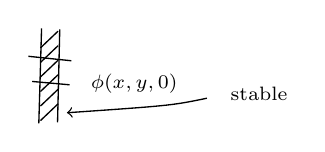
\begin{tikzpicture}[x=.70cm,y=.71cm,line width=.48pt,font=\scriptsize]
\draw (-2.5,-.82)--(-2.45,.88) (-2.16,-.8)--(-2.12,.86);
\foreach \y in {-.77,-.51,-.25,.01,.27,.53} {
  \draw (-2.47,\y)--(-2.15,{\y+.30});
}
\draw (-2.69,.38)--(-1.91,.30) (-2.62,-.07)--(-1.94,-.13);
\draw[->] (.55,-.37) .. controls (-.09,-.50) .. (-1.99,-.63);
\node at (-.77,-.11) {$\phi(x,y,0)$};
\node[anchor=west] at (.80,-.29) {\uwave{stable}};
\end{tikzpicture}}\endgroup}
\end{GelfandAdjacentEvidence}
\begin{GelfandAdjacentEvidence}{GELFAND-P001034}{9}

\SourceFigure{GELFAND-P001034}{closed-string}{%
\begingroup\color{black}\GelfandFitDiagram{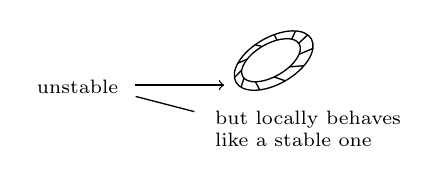
\begin{tikzpicture}[x=.69cm,y=.69cm,line width=.48pt,font=\scriptsize]
\node[anchor=west] at (-3.18,.15) {\uwave{unstable}};
\draw[->] (-1.2,.19)--(.45,.19);
\draw (-1.18,-.02)--(-.10,-.30);
\begin{scope}[shift={(1.36,.64)},rotate=30]
\draw (0,0) ellipse [x radius=.80,y radius=.43];
\draw (-.04,.03) ellipse [x radius=.60,y radius=.30];
\foreach \a in {3,29,62,91,128,158,187,222,260,293,327} {
  \draw ({-.04+.60*cos(\a)},{.03+.30*sin(\a)}) --
        ({.80*cos(\a+10)},{.43*sin(\a+10)});
}
\end{scope}
\node[anchor=west,align=left] at (.10,-.62) {but locally behaves\\like a stable one};
\end{tikzpicture}}\endgroup}
\end{GelfandAdjacentEvidence}
\begin{GelfandAdjacentEvidence}{GELFAND-P001034}{10}


One can require the thread to satisfy the equation of mo-
\SourceFigure{GELFAND-P001034}{bottom-continuation}{The word breaks off at “mo-” at the end of the frame.}
\end{GelfandAdjacentEvidence}



\Needspace{7\baselineskip}
\begin{GelfandAdjacentEvidence}{GELFAND-P001035}{1}
\SourcePage{GELFAND-P001035}{unlabelled}
\dashuline{Wonders with a thread}: \uwave{there is a notion of topological nontriviality}.

(11) \dashuline{Thread}: the field \uwave{\(\phi(x,y,t)\)}
\quad (i.e. it depends on only two spatial variables)

\Unclear{GELFAND-P001035}{energy-cancel}{Illegible cancelled entry before the abbreviated “functional.”}
\end{GelfandAdjacentEvidence}
\begin{GelfandAdjacentEvidence}{GELFAND-P001035}{2}

The energy functional per unit of the coordinate $z$ must be finite.
\[
\int\mathcal E(x,y)\,dx\,dy<\infty
\]
\SourceFigure{GELFAND-P001035}{energy-abbreviation}{The manuscript abbreviates “functional” as «ф-л».}
\end{GelfandAdjacentEvidence}
\begin{GelfandAdjacentEvidence}{GELFAND-P001035}{3}


($\mathcal E$ --- density, gives the energy)
\SourceFigure{GELFAND-P001035}{density-gloss}{The gloss reads “density, gives the energy.”}
\end{GelfandAdjacentEvidence}
\begin{GelfandAdjacentEvidence}{GELFAND-P001035}{4}


In (10) the region where the field is nontrivial is hatched.

(as $e^{-\alpha x^2}$ is concentrated in a region of size $1/\sqrt{\alpha}$).

(12)
\SourceFigure{GELFAND-P001035}{circle-linking-thread}{%
\begingroup\color{black}\GelfandFitDiagram{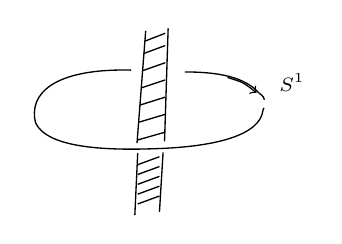
\begin{tikzpicture}[x=.92cm,y=.78cm,line width=.48pt,font=\scriptsize]
\draw (-.17,-1.54)--(-.13,-.53) (-.14,-.37)--(-.02,1.46);
\draw (.17,-1.49)--(.22,-.52) (.24,-.34)--(.29,1.50);
\foreach \y in {-.32,-.03,.25,.53,.81,1.09,1.29} {
  \draw ({-.14+.064*(\y+.37)},\y)--(.25,{\y+.13});
}
\foreach \y in {-1.36,-1.20,-1.04,-.88,-.72} {
  \draw (-.13,\y)--(.17,{\y+.13});
}
\draw (-.22,.82) .. controls (-1.31,.85) and (-1.64,.42) .. (-1.54,-.04)
  .. controls (-1.38,-.44) and (-.61,-.49) .. (.10,-.46)
  .. controls (.95,-.43) and (1.56,-.24) .. (1.60,.17);
\draw (.52,.79) .. controls (1.12,.79) and (1.39,.65) .. (1.55,.44);
\draw[dashed] (1.55,.44) .. controls (1.65,.37) and (1.64,.25) .. (1.60,.17);
\draw[->] (1.11,.70) .. controls (1.33,.62) .. (1.51,.45);
\node at (2.00,.62) {$S^1$};
\end{tikzpicture}}\endgroup}
\end{GelfandAdjacentEvidence}
\begin{GelfandAdjacentEvidence}{GELFAND-P001035}{5}

\SourceFigure{GELFAND-P001035}{circle-map}{%
We obtain a map $S^1\to\mathcal R$.\par
$\Rightarrow$ stability (?)}
\end{GelfandAdjacentEvidence}
\begin{GelfandAdjacentEvidence}{GELFAND-P001035}{6}


(13) \uwave{On going around a thread, a particle may change type (become another particle)}

\dashuline{Example}: it may change its electric charge.
\SourceFigure{GELFAND-P001035}{parallel-strokes}{$\vert\quad\vert$}
\end{GelfandAdjacentEvidence}
\begin{GelfandAdjacentEvidence}{GELFAND-P001035}{7}


$\forall$ vacuum $\phi\in\mathcal R$ $\exists$ a group of unbroken symmetries $H_\phi$ (preserving $\phi$)

\dashuline{Assumption}:
\begin{equation*}
H_\phi=K\times U(1)\subset\widetilde G
\tag{14}
\end{equation*}
(here $U(1)$ --- the electromagnetic group).

Let $\widetilde G$ contain an element $\alpha\in\widetilde G$, which reverses $U(1)$:
\begin{equation*}
\text{\uwave{\(\alpha u\alpha^{-1}=u^{-1}\)}}\qquad \text{for }u\in U(1)
\tag{15}
\end{equation*}

(16) \underline{Claim.} Then $\exists$ a topologically nontrivial thread (and even a solution) around which a particle changes its charge.

\begin{center}--- $\cdot$ ---\end{center}

On parity.
\Unclear{GELFAND-P001035}{mirror-cancel}{The crossed-out mark is illegible.}
\end{GelfandAdjacentEvidence}
\begin{GelfandAdjacentEvidence}{GELFAND-P001035}{8}

Hypothesis: mirror matter exists.
\SourceFigure{GELFAND-P001035}{mirror-abbreviation}{“On parity,” then the abbreviation for “Hypothesis.”}
\end{GelfandAdjacentEvidence}
\begin{GelfandAdjacentEvidence}{GELFAND-P001035}{9}


Inside the Sun there is a planet made of mirror matter. It interacts weakly but exerts a gravitational influence $\Rightarrow$ this explains certain experiments.

(17) \underline{Claim.} 1) $\exists$ grand unifications that include mirror particles

2) Illegible cancelled entry after “2).”\textsuperscript{?}
\Unclear{GELFAND-P001035}{cancel17}{Illegible cancelled entry after “2).”}
\end{GelfandAdjacentEvidence}
\begin{GelfandAdjacentEvidence}{GELFAND-P001035}{10}

$\exists$ threads around which particles turn into mirror particles.

The interaction of our particles with mirror particles is \uwave{weak} (interaction through heavy bosons; if we neglect it --- the Lagrangian splits).
\SourceFigure{GELFAND-P001035}{overwritten-prefix}{The start of “neglect” is written over earlier strokes.}
\end{GelfandAdjacentEvidence}
\begin{GelfandAdjacentEvidence}{GELFAND-P001035}{11}


These are \underline{not} antiparticles. There are mirror photons, mirror charge, and so on.

\uwave{The coupling is very weak}.

\uwave{Thread of such unifications}. Effect.
\SourceFigure{GELFAND-P001035}{thread-heading}{The manuscript underlines “Thread of such unifications.”}
\end{GelfandAdjacentEvidence}
\begin{GelfandAdjacentEvidence}{GELFAND-P001035}{12}


\SourceFigure{GELFAND-P001035}{star-thread-observer}{%
\begingroup\color{black}\GelfandFitDiagram{\begin{tikzpicture}[x=.83cm,y=.79cm,line width=.52pt,font=\scriptsize]
\draw (-.14,1.67)--(.14,1.67)
      (-.09,1.52)--(.09,1.81) (-.09,1.81)--(.09,1.52);
\node[anchor=west] at (.19,1.69) {star};
\draw (-1.0,-.06)--(2.92,1.27);
\node[anchor=west] at (2.97,1.30) {Thread};
\fill (1.71,-.39) circle (.032);
\node[anchor=west] at (1.79,-.32) {us};
\end{tikzpicture}}\endgroup}
\end{GelfandAdjacentEvidence}
\begin{GelfandAdjacentEvidence}{GELFAND-P001035}{13}

We stop seeing the star because its photons
\Unclear{GELFAND-P001035}{cancel-bottom}{Illegible cancelled entry before the abbreviated “become.”}
\end{GelfandAdjacentEvidence}
\begin{GelfandAdjacentEvidence}{GELFAND-P001035}{14}

become mirror photons.

The dynamics is semiclassical, which applies because we are far from the thread.

The threads are thought to have survived from the early universe.
\SourceFigure{GELFAND-P001035}{last-verb}{The last sentence begins “It is thought.”}
\end{GelfandAdjacentEvidence}



\Needspace{7\baselineskip}
\begin{GelfandAdjacentEvidence}{GELFAND-P001036}{1}
\SourcePage{GELFAND-P001036}{8}
It is unclear whether there are \underline{quantum-mechanically} stable threads (classically they are stable).

As the thread moves, the stars should be replaced (by mirror ones).
\SourceFigure{GELFAND-P001036}{line-02-verb}{The verb means “to be replaced.”}
\end{GelfandAdjacentEvidence}
\begin{GelfandAdjacentEvidence}{GELFAND-P001036}{2}

\SourceFigure{GELFAND-P001036}{line-02-parenthesis}{In parentheses: “by mirror ones.”}
\end{GelfandAdjacentEvidence}
\begin{GelfandAdjacentEvidence}{GELFAND-P001036}{3}


\uwave{Khlopov}: metagalaxies in half [tentative reading]\textsuperscript{?}
\Unclear{GELFAND-P001036}{line-03-phrase}{metagalaxies in half [tentative reading]}
\end{GelfandAdjacentEvidence}
\begin{GelfandAdjacentEvidence}{GELFAND-P001036}{4}

and nothing will change;
the only chance --- quasars; they are
special [tentative reading]\textsuperscript{?},
\Unclear{GELFAND-P001036}{line-04-adjective}{special [tentative reading]}
\end{GelfandAdjacentEvidence}
\begin{GelfandAdjacentEvidence}{GELFAND-P001036}{5}

but they have a characteristic rhythm of variation.

There is a \underline{preprint}: one quasar over 100 years
\uwave{sharply changed its luminosity}.
\SourceFigure{GELFAND-P001036}{preprint-or-precedent}{The underlined word reads “preprint.”}
\end{GelfandAdjacentEvidence}


\dashuline{Khlopov's remark}: it is ex\underline{plained}, \underline{if} a thread passed.


\Needspace{7\baselineskip}
\begin{GelfandAdjacentEvidence}{GELFAND-P001037}{1}
\SourcePage{GELFAND-P001037}{unlabelled}
\underline{20/$\overline{\underline{\mathrm{IX}}}$-82.}\qquad \uuline{Gelfand Seminar.}

\uuline{Sinai.}

\underline{Topics} (in physics)

1. Renormalization group.

2. Debye screening as the principal mechanism of phase transitions in systems with continuous symmetry.

3. Gauge models.

4. Gravity, supersymmetry, supergravity.

\uuline{A. A. Migdal.}

5. Lattice models.
\Unclear{GELFAND-P001037}{topic-five-cancellation}{Illegible cancelled expression in parentheses.}
\end{GelfandAdjacentEvidence}
\begin{GelfandAdjacentEvidence}{GELFAND-P001037}{2}


6. Strings.

7. Large $N$ ($N$ --- rank of the gauge group):
\[
u(\infty)=\mathrm{sp}(\infty)=O(\infty)
\]
\SourceFigure{GELFAND-P001037}{large-n-symbols}{Manuscript notation: \(u(\infty),\mathrm{sp}(\infty),O(\infty)\).}
\end{GelfandAdjacentEvidence}
\begin{GelfandAdjacentEvidence}{GELFAND-P001037}{3}


8. Quarks and leptons. \dashuline{Unified} theories.

9. Anderson localization.

10. Feigenbaum universality.
\SourceFigure{GELFAND-P001037}{feigenbaum-overwrite}{The \(n\) in the handwritten surname “Feigenbaum” is written over earlier strokes.}
\end{GelfandAdjacentEvidence}


\uuline{Sinai} \underline{on item 10.}

\uwave{In the one-dimensional case}: Let
\[
\begin{aligned}
[-1,1]&\longrightarrow[-1,1]\\
x&\longmapsto f(x;\mu)
\end{aligned}
\]
\[
\begin{aligned}
\text{a)}\quad &f(-x;\mu)=f(x;\mu)\\
\text{b)}\quad &f(0;\mu)=1.
\end{aligned}
\]
[At right:] \underline{Example}: $f(x,\mu)=1-\mu x^2$, $1<\mu<2$.


\Needspace{7\baselineskip}
\begin{GelfandAdjacentEvidence}{GELFAND-P001038}{1}
\SourcePage{GELFAND-P001038}{9}
\Unclear{GELFAND-P001038}{top-cancellation}{The cancelled word may be the abbreviation for “Consider.”}
\end{GelfandAdjacentEvidence}
\begin{GelfandAdjacentEvidence}{GELFAND-P001038}{2}

[inserted above the line] There is a sequence of values $\mu_n$:
\begin{equation*}
\forall\mu:\quad \mu_n<\mu<\mu_{n+1}\quad\Rightarrow\quad
\exists\ \text{a stable orbit of period }2^n.
\tag{1}
\end{equation*}
Consider
\begin{equation*}
\frac{\mu_n-\mu_{n+1}}{\mu_{n-1}-\mu_n}
\underset{n\to\infty}{\longrightarrow}\delta^{-1},\qquad
\delta\approx4{,}6992
\tag{2}
\end{equation*}
\SourceFigure{GELFAND-P001038}{feigenbaum-constant}{The manuscript reads \(\delta\approx4{,}6992\).}
\end{GelfandAdjacentEvidence}
\begin{GelfandAdjacentEvidence}{GELFAND-P001038}{3}


The set of [inserted above the line] families of maps for which $\exists$ a sequence $\mu_n$ ---
\underline{an open set} in the space of maps.
\SourceFigure{GELFAND-P001038}{family-insertion}{The abbreviation for “families,” with an insertion mark.}
\end{GelfandAdjacentEvidence}
\begin{GelfandAdjacentEvidence}{GELFAND-P001038}{4}


\uwave{There is a generalization for differential equations}.

\begin{equation*}
\frac{dx_i}{dt}=f(x_1,\ldots,x_r,\mu),\qquad1\le i\le r
\tag{3}
\end{equation*}
\Unclear{GELFAND-P001038}{sinai-eq3-indices}{The subscript of the last \(x\) resembles the \(r\) in the upper bound. The strokes are small.}
\end{GelfandAdjacentEvidence}
\begin{GelfandAdjacentEvidence}{GELFAND-P001038}{5}


(4) $\mu_n$, $\mu_n<\mu<\mu_{n+1}$ $\Rightarrow$ there is a periodic orbit attracting everything,
except a finite number of closed orbits.

\SourceFigure{GELFAND-P001038}{orbit-progression}{%
\begingroup\color{black}\GelfandFitDiagram{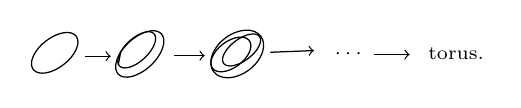
\begin{tikzpicture}[x=.75cm,y=.72cm,font=\scriptsize,line width=.45pt]
\draw[rotate around={38:(-3.41,0)}] (-3.41,0) ellipse [x radius=.46,y radius=.26];
\draw[->] (-2.90,-.06)--(-2.46,-.06);
\begin{scope}[shift={(-1.97,-.02)},rotate=43]
\draw (0,0) ellipse [x radius=.50,y radius=.28];
\draw (.01,.09) ellipse [x radius=.40,y radius=.20];
\draw (-.39,.12)--(-.22,.25);
\end{scope}
\draw[->] (-1.39,-.05)--(-.87,-.05);
\begin{scope}[shift={(-.32,-.02)},rotate=37]
\draw (0,0) ellipse [x radius=.50,y radius=.35];
\draw (-.09,.06) ellipse [x radius=.39,y radius=.23];
\draw (.10,.01) ellipse [x radius=.38,y radius=.19];
\end{scope}
\draw[->] (.24,.01)--(.98,.04);
\node at (1.56,-.02) {$\cdots$};
\draw[->] (2.00,-.03)--(2.60,-.03);
\node[anchor=west] at (2.75,-.02) {\uwave{torus}.};
\end{tikzpicture}}\endgroup\par
The exact joins in the two middle contours are unclear.}
\end{GelfandAdjacentEvidence}
\begin{GelfandAdjacentEvidence}{GELFAND-P001038}{6}


\begin{equation*}
\mu_n-\mu_\infty\sim C(f)\delta^{-n},
\tag{5}
\end{equation*}
where $\delta$ --- the same as above,
and the set of such systems is \uwave{open}.

\uwave{More parameters.}

(6) $\mu_1,\mu_2$ $\Rightarrow$ \uwave{period tripling occurs}
(and one also finds a $\mathrm{const}$).

\begin{center}--- $\cdot$ ---\end{center}

For the function $f$ there is a complicated functional equation:
\begin{equation*}
-\frac1\alpha f(f(\alpha x))=f(x)
\tag{7}
\end{equation*}
\uwave{It is solved}: with a polynomial (degree 10) and numerically on a computer.

The renormalization group arises from linearizing this equation.

(8) \underline{Question}: what happens when $\mu>\mu_\infty$ for the vector field?

For maps, it is known that a map with an ergodic invariant measure arises
(mixing and so forth $\Rightarrow$ onset of stochasticity).

\uuline{A. A. Migdal.}

Given a field $\varphi(x)$ with values in the algebra $u(N)$, i.e. $(\varphi_{ij})$ ---
an anti-Hermitian matrix,
\begin{equation*}
\varphi_{ij}(x)=-\varphi_{ji}^{*}(x)\qquad\text{or}\qquad
\varphi(x)=-\varphi^{+}(x),\qquad\text{(for definiteness)}
\tag{1}
\end{equation*}

As $N\to\infty$ there is a [inserted above the line] universal limit
(non-Gaussian!) and for the limit there are certain equations and
\Unclear{GELFAND-P001038}{migdal-prose-cancellation}{Illegible cancelled entry before “observations.”}
\end{GelfandAdjacentEvidence}
\begin{GelfandAdjacentEvidence}{GELFAND-P001038}{7}

observations.
\SourceFigure{GELFAND-P001038}{universal-insertion}{The abbreviation for “universal” is inserted above the line.}
\end{GelfandAdjacentEvidence}


\begin{equation*}
L=\operatorname{tr}\left[\frac12(\partial_\mu\varphi)^2+U(\varphi)\right]N/\lambda,
\tag{2}
\end{equation*}
$U(\varphi)$ --- a polynomial of degree 4 --- for example, $\varphi^4$.

(3) $\bullet$ The classical equation $\dfrac{\delta S}{\delta\varphi}=0$, where
\begin{equation*}
S=\int L\,d^4x
\tag{4}
\end{equation*}
(the space is Euclidean)


\Needspace{7\baselineskip}
\begin{GelfandAdjacentEvidence}{GELFAND-P001039}{1}
\SourcePage{GELFAND-P001039}{unlabelled}
Consider the equation
\begin{equation*}
\frac{\partial\varphi}{\partial\tau}+\frac{\delta S}{\delta\varphi}=J(x,\tau),
\tag{5}
\end{equation*}
\SourceFigure{GELFAND-P001039}{noise-under-j}{%
$\underset{\text{random current }=\text{ Gaussian random noise}}{\uparrow}$}
\end{GelfandAdjacentEvidence}
\begin{GelfandAdjacentEvidence}{GELFAND-P001039}{2}


where
\begin{equation*}
\langle J^{ik}(x,\tau)J^{i'k'}(x',\tau')\rangle
=\delta^{ii'}\delta^{kk'}\delta(x-x')\delta(\tau-\tau')
\tag{6}
\end{equation*}
(this describes them completely, since they are Gaussian)

(7) \underline{Claim.} Let $\varphi|_{\tau=0}=0$.
Then the solution $\varphi(x,\tau)$ has the property that if
\[
\overline Q=\frac1T\int_0^T Q(\varphi(x,\tau))\,d\tau
\]
[At right:] ($Q$ --- a functional; e.g. $Q=\operatorname{tr}(\varphi^2)$).
invariant under the group for the adjoint action
\[
\varphi\longmapsto S^{+}\varphi S
\]
then $\overline Q$ is given by the formula
\begin{equation*}
\overline Q=\int D\varphi\,\exp(-S)\,Q(\varphi(x))\Big/\int D\varphi\,e^{-S}
\tag{8}
\end{equation*}

Instead of (8) we consider (5).

\textcircled{1}\quad \uwave{Self-averaging}. Consider
\begin{equation*}
G(1,\ldots,n)=\frac{\operatorname{tr}}N(\varphi(1)\ldots\varphi(n))
\tag{9}
\end{equation*}
Here $(T,x_1)\mapsto1$, $\ldots$ (for brevity);
\underline{$T$ is fixed}.
\Unclear{GELFAND-P001039}{short-time-correction}{The first character in the pair is overwritten and most likely reads \(T\).}
\end{GelfandAdjacentEvidence}
\begin{GelfandAdjacentEvidence}{GELFAND-P001039}{3}


Then
\begin{equation*}
\lim_{T\to\infty}G_T(1,\ldots,n,T)=\overline G+O(1/N),
\qquad\text{(as }N\to\infty\text{)}
\tag{10}
\end{equation*}
\Unclear{GELFAND-P001039}{eq10-raised-sign}{A mark beside the base of \(G\) resembles \(T\). After \(n\) there is an oblique stroke and a raised mark resembling \(T\).}
\end{GelfandAdjacentEvidence}
\begin{GelfandAdjacentEvidence}{GELFAND-P001039}{4}


[At right:] here $\overline G(1,\ldots,n)$ --- a function of the points, independent of $T$ and $N$.

(decrease in fluctuations).

\uwave{The points coincide}:
$\dfrac1N\operatorname{tr}\varphi^n=\dfrac1N\sum_\lambda\lambda^n$ and the variance decreases.

In general there arises a $\sum$ of terms with identical probability distributions.

Thus: traces \uwave{do not fluctuate}.

\textcircled{2}\quad At $N=\infty$ a reduction is possible:
\begin{equation*}
\varphi(x)\longmapsto e^{ipx}\varphi(0)e^{-ipx},\qquad
p=i\,\partial/\partial x
\tag{11}
\end{equation*}
$p$ An illegible mark after \(p\) is crossed out.\textsuperscript{?}
\Unclear{GELFAND-P001039}{after-p-cancellation}{An illegible mark after \(p\) is crossed out.}
\end{GelfandAdjacentEvidence}
\begin{GelfandAdjacentEvidence}{GELFAND-P001039}{5}

can be replaced by a matrix in the Cartan algebra (diagonal)

\begin{equation*}
\widetilde J(x,t)=e^{ip_\mu x^\mu}j(t)e^{-ip_\mu x^\mu},
\tag{12}
\end{equation*}
\Unclear{GELFAND-P001039}{eq12-x-corrections}{In both exponents the \(x\) subscripts are crossed out and \(\mu\) is written above. The cancelled subscripts are illegible.}
\end{GelfandAdjacentEvidence}
\begin{GelfandAdjacentEvidence}{GELFAND-P001039}{6}


[At right:] $p_\mu$ --- a diagonal matrix,
$p=\operatorname{diag}(p_\mu^1,\ldots,p_\mu^N)$

$j(t)$ --- Gaussian noise

\SourceFigure{GELFAND-P001039}{repeated-noise-arrow}{%
$j(t)$ --- Gaussian noise. \quad $\swarrow$ to (13)}
\end{GelfandAdjacentEvidence}
\begin{GelfandAdjacentEvidence}{GELFAND-P001039}{7}


\Unclear{GELFAND-P001039}{random-p-cancellation}{A cancelled entry on the right begins with \(p\).}
\end{GelfandAdjacentEvidence}
\begin{GelfandAdjacentEvidence}{GELFAND-P001039}{8}

$p^\mu$ --- a random quantity (independent of both $t$, and $x$)
\Unclear{GELFAND-P001039}{random-p-indices}{The superscript resembles \(\mu\). The lower stroke may be a cancelled index.}
\end{GelfandAdjacentEvidence}


\begin{equation*}
\langle j^{ik}(t),j^{i'k'}(t')\rangle=\delta(t-t')\delta^{ii'}\delta^{kk'}
\tag{13}
\end{equation*}


\Needspace{7\baselineskip}
\begin{GelfandAdjacentEvidence}{GELFAND-P001040}{1}
\SourcePage{GELFAND-P001040}{10}
$p^j$ --- random variables, distributed [inserted above] (according to a Gaussian law)
with density $\exp(-p^2/\Lambda^2)$ (with variance $1/\Lambda^2$)
\Unclear{GELFAND-P001040}{top-p-index}{The superscript resembles \(j\). It may be \(i\).}
\end{GelfandAdjacentEvidence}
\begin{GelfandAdjacentEvidence}{GELFAND-P001040}{2}

\SourceFigure{GELFAND-P001040}{top-density-variance}{The manuscript gives \(\exp(-p^2/\Lambda^2)\) and “with variance \(1/\Lambda^2\).”}
\end{GelfandAdjacentEvidence}
\begin{GelfandAdjacentEvidence}{GELFAND-P001040}{3}


where $\underset{\substack{\vert\\\text{\uwave{cutoff radius}}}}{\Lambda}\to\infty$
(after $N\to\infty$).

In the limit as
\[
\begin{gathered}
N\to\infty\\
\Lambda\to\infty
\end{gathered}
\]
we get the same white noise $J(x,t)$ (see above).

It reduces to an ordinary equation (a random matrix).

\SourceFigure{GELFAND-P001040}{equivalence-cancellation}{\sout{Equivalence}}
\end{GelfandAdjacentEvidence}
\begin{GelfandAdjacentEvidence}{GELFAND-P001040}{4}


\underline{Assertion}.
\[
\underset{\substack{\vert\\\text{with }J}}{G}
-\underset{\substack{\vert\\\text{with }\widetilde J}}{\widetilde G}
\to0
\]
\begin{equation*}
\frac{\partial\widetilde\varphi}{\partial\tau}
+\frac{\delta S}{\delta\widetilde\varphi}=\widetilde J(x,\tau)
\tag{14}
\end{equation*}

The solution is:
\begin{equation*}
\varphi(x,\tau)=e^{ipx}\bar\varphi(t)e^{-ipx},\qquad\text{where}
\tag{15}
\end{equation*}
\SourceFigure{GELFAND-P001040}{eq15-time}{The left side uses \(\tau\). The argument of \(\bar\varphi\) is \(t\).}
\end{GelfandAdjacentEvidence}
\begin{GelfandAdjacentEvidence}{GELFAND-P001040}{5}


\begin{equation*}
\frac{\partial\bar\varphi}{\partial\tau}
+[p[p\bar\varphi]]+U(\bar\varphi)=\widetilde j
\tag{16}
\end{equation*}
\SourceFigure{GELFAND-P001040}{eq16-notation}{There are no visible commas in the brackets or prime on \(U\).}
\end{GelfandAdjacentEvidence}
\begin{GelfandAdjacentEvidence}{GELFAND-P001040}{6}


\[
p=\operatorname{diag}(p_1,\ldots,p_N)
\]
Thus the dependence on the coordinates has been eliminated.

The integrals pass into the integral:
\begin{equation*}
\bar Q=\int dp\int d\varphi\,\exp\bigl(\operatorname{tr}\bigl(([p,\varphi]^2+U_\Lambda(\varphi)\bigr)\bigr)Q(\varphi)
\tag{17}
\end{equation*}
\SourceFigure{GELFAND-P001040}{eq17-parentheses}{One opening parenthesis after \(\exp\), two after \(\operatorname{tr}\), and three closing ones after \(\varphi\) in \(U_\Lambda(\varphi)\).}
\end{GelfandAdjacentEvidence}
\begin{GelfandAdjacentEvidence}{GELFAND-P001040}{7}


More precisely,

\Unclear{GELFAND-P001040}{crossed-before-eq18}{The cancelled line may have started with \((18)\) and \(\bar Q\).}
\end{GelfandAdjacentEvidence}
\begin{GelfandAdjacentEvidence}{GELFAND-P001040}{8}

\begin{equation*}
\begin{aligned}
\underset{\substack{\uparrow\\\text{along trajectories (see above)}}}{\bar Q}
&=\lim_{\Lambda\to\infty}\lim_{N\to\infty}M_p\\
&\quad\Bigl\{\int_{U(N)}d\varphi\,\exp\bigl(\operatorname{tr}\bigl(([p,\varphi]^2+U(\varphi)\bigr)\bigr)Q(\varphi)\Bigr\}
\end{aligned}
\tag{18}
\end{equation*}
\SourceFigure{GELFAND-P001040}{eq18-parentheses}{The parentheses follow the same pattern as in (17).}
\end{GelfandAdjacentEvidence}
\begin{GelfandAdjacentEvidence}{GELFAND-P001040}{9}


\underline{To be calculated}:
\begin{equation*}
\lim_{N\to\infty}\frac{1}{N^2}\ln
\int_{U(N)}\prod_{\mu=1}^{4}dU_\mu\,
\exp\bigl(-\beta N\sum_{\mu,\nu}\operatorname{tr}(U_\mu U_\nu U_\mu^+U_\nu^+)\bigr)=F(\beta)
\tag{19}
\end{equation*}
\SourceFigure{GELFAND-P001040}{log-insertion}{The manuscript inserts \(\tfrac{1}{N^2}\ln\) before the integral.}
\end{GelfandAdjacentEvidence}
\begin{GelfandAdjacentEvidence}{GELFAND-P001040}{10}

(free energy)

$dU_\mu$ --- Haar measure

(Partition function of lattice theory [inserted above] (field) as $N\to\infty$ in four-dimensional space)

This is $\sim$ field theory

\underline{Evaluated}:
\begin{equation*}
\int dU\,\exp\bigl(\beta N\operatorname{tr}(Uh+h^+U^+)
\tag{20}
\end{equation*}
for an arbitrary matrix $h$
\SourceFigure{GELFAND-P001040}{eq20-parentheses}{Only one closing parenthesis is visible at the end of the formula.}
\end{GelfandAdjacentEvidence}
\begin{GelfandAdjacentEvidence}{GELFAND-P001040}{11}


(a complicated expression)

First. \uwave{Pirizen}, \uwave{Gross}; then \uwave{Fateev}.
\Unclear{GELFAND-P001040}{bottom-surname}{The first surname appears to read “Pirizen.” Its first vowel is unclear.}
\end{GelfandAdjacentEvidence}



\Needspace{7\baselineskip}
\begin{GelfandAdjacentEvidence}{GELFAND-P001041}{1}
\SourcePage{GELFAND-P001041}{unlabelled}
\underline{27/$\overline{\underline{\mathrm{IX}}}$-82 {}}\qquad
\uuline{Gelfand Seminar.}

\uuline{Fuchs.}

\uwave{Representations of the diffeomorphism group of the circle}.

(1) Consider the algebra $\{e_i,\ i\in\mathbb Z\}$
\[
\relax[e_i,e_j]=(j-i)e_{i+j}.
\]
(of vector fields on the circle)
\SourceFigure{GELFAND-P001041}{cancelled-algebra-name}{%
[At right:] \sout{(Virasoro alg.)}}
\end{GelfandAdjacentEvidence}
\begin{GelfandAdjacentEvidence}{GELFAND-P001041}{2}


There is a unique central extension (Gelfand–Fuchs):
\begin{equation*}
\{e_i,z\},\quad
\left.
\begin{gathered}
\relax[e_i,e_j]=\begin{cases}
(j-i)e_{i+j},&i+j\ne0,\\
\text{---''---}+\frac{1}{12}(j^3-j)z,&i+j=0,
\end{cases}\\
[e_i,z]=0,\quad\forall i
\end{gathered}
\right]\quad\begin{gathered}\text{Virasoro}\\\text{algebra}\end{gathered}
\tag{2}
\end{equation*}

\dashuline{Representations of the Virasoro algebra}.

(3) \uwave{Verma modules},
\SourceFigure{GELFAND-P001041}{verma-grading}{%
\begingroup\color{black}\GelfandFitDiagram{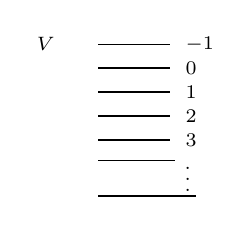
\begin{tikzpicture}[x=.85cm,y=.82cm,font=\scriptsize,line width=.50pt]
\node at (-.78,.01) {$V$};
\foreach \y/\weight in {0/-1,-.37/0,-.74/1,-1.11/2,-1.48/3} {
  \draw (0,\y)--(1.08,\y);
  \node[anchor=west] at (1.16,\y) {$\weight$};
}
\draw (0,-1.80)--(1.15,-1.80);
\node at (1.34,-1.97) {$\vdots$};
\draw (0,-2.35)--(1.46,-2.35);
\end{tikzpicture}}\endgroup}
\end{GelfandAdjacentEvidence}
\begin{GelfandAdjacentEvidence}{GELFAND-P001041}{3}

graded The cancelled mark is illegible.\textsuperscript{?}
\Unclear{GELFAND-P001041}{verma-overwritten-mark}{The cancelled mark is illegible.}
\end{GelfandAdjacentEvidence}
\begin{GelfandAdjacentEvidence}{GELFAND-P001041}{4}

modules bounded below

(graded and bounded on one side)

(4) Subalgebra $\{e_i,\ i>0\}$;

\underline{Verma module}: if there is [inserted above] a vector $v$, such that
\SourceFigure{GELFAND-P001041}{basis-insertion}{\sout{a basis}}
\end{GelfandAdjacentEvidence}
\begin{GelfandAdjacentEvidence}{GELFAND-P001041}{5}

\[
\{v,\ e_1v,\ e_1^2v,\ e_2v,\ e_1^3v,\ e_2e_1v,\ e_3v,\ \ldots\}\quad\text{---}
\]

(5) --- a basis, and $e_{-j}v=0$ for $j>0$.
(it suffices that $e_{-1}v=e_{-2}v=0$)

Fix complex numbers $h$ and $c$.
\begin{equation*}
\underline{e_0v=hv,\quad zv=cv}
\tag{6}
\end{equation*}
(additional condition). ---

From $h,c$ it is recovered uniquely. Notation $V_{h,c}$.

\uwave{Construct a module} $\{f_j\mid j\in\mathbb Z\}$
\Unclear{GELFAND-P001041}{module-horizontal-marks}{Two strokes appear above the entry, one to the right of \(f_j\) and one above \(\mathbb Z\). Their relation to the entry is unclear.}
\end{GelfandAdjacentEvidence}
\begin{GelfandAdjacentEvidence}{GELFAND-P001041}{6}

(auxiliary) by the formulas:
\begin{equation*}
e_if_j=[j+\mu-(i+1)\lambda]f_{i+j}
\tag{7}
\end{equation*}

(\uwave{One can picture}:
\begin{equation*}
e_i=z^{i+1}\frac{d}{dz},\quad f_j=z^{j+\mu}dz^{-\lambda})
\tag{8}
\end{equation*}
Denote it by $\overline W_{\lambda,\mu}$
\SourceFigure{GELFAND-P001041}{module-symbol}{A bar is visible over \(W\).}
\end{GelfandAdjacentEvidence}
\begin{GelfandAdjacentEvidence}{GELFAND-P001041}{7}


Consider the sequences.
\begin{equation*}
\begin{gathered}
\cdots\wedge f_{j_3}\wedge f_{j_2}\wedge f_{j_1}\\
\cdots<j_3<j_2<j_1
\end{gathered}
\tag{9}
\end{equation*}
\[
\cdots\wedge f_{-4}\wedge\underset{-3}{f_2}\wedge\underset{-2}{f_5}\wedge\underset{-1}{f_9}
\]
\SourceFigure{GELFAND-P001041}{wedge-last-index}{The final factor is \(f_9\), with \(-1\) beneath it.}
\end{GelfandAdjacentEvidence}
\begin{GelfandAdjacentEvidence}{GELFAND-P001041}{8}


(the numbers run consecutively up to a certain point; if the subsequent ones are replaced by

consecutive ones, then The short cancelled entry is illegible.\textsuperscript{?}
\Unclear{GELFAND-P001041}{bottom-cancelled-mark}{The short cancelled entry is illegible.}
\end{GelfandAdjacentEvidence}

it ends at $-1$

$e_i$ is applied successively from the right; one obtains a sum of infinitely many terms.

If the resulting $f_{i+j}$ is already present, the product is $0$.


\Needspace{7\baselineskip}
\begin{GelfandAdjacentEvidence}{GELFAND-P001042}{1}
\SourcePage{GELFAND-P001042}{11}

In fact, one obtains a finite sum.

This defines $e_i$ for $i\ne0$, and $e_0$ cannot be defined this way.

\[
e_0=[e_{-1},e_1]\quad\text{— define by this formula }e_0.
\]
\[
e_0=[e_{-2},e_2]\quad\text{— a different coefficient results! — contradiction.}
\]
\SourceFigure{GELFAND-P001042}{overwritten-e0}{The initial symbol of the second equality has been overwritten and reads as \(e_0\).}
\end{GelfandAdjacentEvidence}
\begin{GelfandAdjacentEvidence}{GELFAND-P001042}{2}


But one can determine $e_0$ and $z$ simultaneously (and uniquely!).

$z$ — multiplication by a number.

(see the work of Feigin and Fuchs; ФА, 1982, $N=2$)

$e_0$ — multiplication by $h+n$,\quad
$h=\tfrac12\mu(\mu-2\lambda+1)$.\quad (?)
\SourceFigure{GELFAND-P001042}{highest-weight-formula}{The manuscript has \(+1\) and “(?)” at right.}
\end{GelfandAdjacentEvidence}
\begin{GelfandAdjacentEvidence}{GELFAND-P001042}{3}


(10) \uwave{Highest-weight vector}:
\[
\underset{\text{(all consecutive)}}{\cdots f_{-3}\wedge f_{-2}\wedge f_{-1}}
\]
If irreducible, then it is a Verma module.

\underline{Kac.}\quad (Lect. Notes Phys., 1979):

Which Verma modules $\overline V_{h,c}$ are irreducible?
\SourceFigure{GELFAND-P001042}{verma-symbol}{A bar appears over \(V\) in the question.}
\end{GelfandAdjacentEvidence}
\begin{GelfandAdjacentEvidence}{GELFAND-P001042}{4}


\begin{equation*}
\begin{aligned}
\overline\Phi_{k_1,k_2}(h,c)
={}&\Bigl(h-\frac{k_1^2-1}{24}(c-13)+\frac{k_1k_2-1}{2}\Bigr)
    \Bigl(h-\frac{k_2^2-1}{24}(c-13)+\frac{k_1k_2-1}{2}\Bigr)+\\
&+\frac{(k_1^2-k_2^2)^2}{16}
\end{aligned}
\tag{11}
\end{equation*}
\SourceFigure{GELFAND-P001042}{kac-polynomial-sign}{A bar over \(\Phi\), and a minus sign before the first fraction.}
\end{GelfandAdjacentEvidence}
\begin{GelfandAdjacentEvidence}{GELFAND-P001042}{5}

\SourceFigure{GELFAND-P001042}{kac-second-factor}{The sign before the last 1 crosses a vertical grid line. It reads as a minus.}
\end{GelfandAdjacentEvidence}
\begin{GelfandAdjacentEvidence}{GELFAND-P001042}{6}


(12) \underline{Thm.} $V_{h,c}$ is reducible
$(\Leftrightarrow)\ \exists$ integers $k_1,k_2>0$,
$\underline{\overline\Phi}_{k_1,k_2}(h,c)=0$.
\Unclear{GELFAND-P001042}{kac-theorem-symbol}{A line is visible below \(\Phi\). The short top stroke may be part of the letterform.}
\end{GelfandAdjacentEvidence}
\begin{GelfandAdjacentEvidence}{GELFAND-P001042}{7}


\begin{center}— . —\end{center}
\[
c=0\quad\Rightarrow\quad h=\frac{m^2-1}{24}
\]
\begin{center}— . —\end{center}

\underline{2nd construction}.

(13) Consider polynomials in the variables
\[
\begin{array}{ccccc}
&x_1,&x_2,&x_3,&\ldots\\
\text{of weights}&1,&2,&3,&\ldots
\end{array}
\]
There are two transformations: multiplication by $x_i$ and $\partial/\partial x_i$.

Set
\begin{equation*}
F_k=\sum_i x_i\frac{\partial}{\partial x_{i+k}}.
\tag{14}
\end{equation*}

Then
\begin{equation*}
e_i=\alpha F_i+
\sum_{\substack{p,q\\p\ne0,\ q\ne0\\p+q=i\\p>q}}F_pF_q
\underset{\text{(if \(i\) is even)}}{\bigl(+\tfrac12 F_{i/2}^{2}\bigr)},
\quad\alpha\text{ — parameter.}
\tag{15}
\end{equation*}
\Unclear{GELFAND-P001042}{eq15-cancelled-coefficient}{Between \(+\) and \(1/2\) there is a cancelled or overwritten mark, possibly a \(2\).}
\end{GelfandAdjacentEvidence}


Here
\begin{equation*}
\alpha=\mu-i(\lambda+\tfrac12)
\tag{16}
\end{equation*}


\Needspace{7\baselineskip}
\begin{GelfandAdjacentEvidence}{GELFAND-P001043}{1}
\SourcePage{GELFAND-P001043}{unlabelled}
\underline{Zamolodchikov.} \underline{(Sasha)}.

(1) Let there be a surface $\vec{x}(\xi^1,\xi^2)$, $\xi^j$ — parameters.

We want to study sums over surfaces of different shapes.

Metric:
\begin{equation*}
G_{ab}=\partial_a\vec{x}\cdot\partial_b\vec{x},\qquad a,b=1,2.
\tag{2}
\end{equation*}
The surface area has the form
\begin{equation*}
A=\int\sqrt{\det G_{ab}}\,d\xi
\tag{3}
\end{equation*}
The expression \(A\) is gauge invariant under $\xi^a\to f^a(\xi)$.

By a choice of gauge one can achieve:
\begin{equation*}
G_{ab}=\rho\delta_{ab}
\tag{4}
\end{equation*}
Equation of motion with Lagrangian $A$:
\begin{equation*}
\partial_a\partial^a\vec{x}=0,\qquad\text{(Laplace equation)}
\tag{5}
\end{equation*}
\begin{equation*}
\begin{cases}
\partial_1\vec{x}\cdot\partial_2\vec{x}=0,\\
(\partial_1\vec{x})^2=(\partial_2\vec{x})^2
\end{cases}
\tag{6}
\end{equation*}
(from (4)).

It suffices to satisfy (6) at the boundary $\Rightarrow$ the solution gives a minimal surface.
\Unclear{GELFAND-P001043}{boundary-abbreviation}{The ending of the abbreviation for “satisfy” has been overwritten. The original strokes are indistinct.}
\end{GelfandAdjacentEvidence}


We want to evaluate, in some sense, the sum
\begin{equation*}
\sum_{\text{surfaces}}e^{-\mu_0^2 A(\text{surface})}
\tag{7}
\end{equation*}
Measure — ?

Consider first
\begin{equation*}
\sum_{\text{paths}}e^{-mL_{\text{path}}}
\tag{8}
\end{equation*}
$L_{\text{path}}$ — length of the path ( in the usual sense; in $d$-dimensional Euclidean space)

For the analogy, introduce a parametrization $\vec{x}(t)$, $t\in(1,2)$. Then
\begin{equation*}
L=\int_1^2\sqrt{(\dot{\vec{x}})^2}\,dt,\qquad
\dot{\vec{x}}=\frac{d\vec{x}}{dt}
\tag{9}
\end{equation*}
Minimizing (9), we get straight lines:
\begin{equation*}
\ddot{\vec{x}}=0\qquad\text{(10) — analogue of (5)}
\tag{10}
\end{equation*}
Freedom (gauge) under substitutions $t\mapsto f(t)$
\begin{equation*}
\begin{cases}
\dot{\vec{x}}=\vec{v}\\
\vec{v}^{\,2}=1
\end{cases}
\qquad\text{(11) — analogue of (6)}
\tag{11}
\end{equation*}


\Needspace{7\baselineskip}
\begin{GelfandAdjacentEvidence}{GELFAND-P001044}{1}
\SourcePage{GELFAND-P001044}{12}
There are several ways to define the integral. They all turn out equivalent in the end.
\Unclear{GELFAND-P001044}{top-equivalence-verb}{The final abbreviation reads as “оказ.” and may read “окаж.”. Both suggest “turn out.”}
\end{GelfandAdjacentEvidence}
\begin{GelfandAdjacentEvidence}{GELFAND-P001044}{2}


(12) \shortstack[l]{\uwave{One:}\\\uwave{method}}
\quad\uwave{replace \(R^d\) by a lattice}.
\[
x^\mu=0,\pm1,\pm2,\ldots
\]
Length \(=\) number of steps.

The sum converges and can be evaluated by elementary means (explicitly!)

(13) \shortstack[l]{\uwave{Another}\\\uwave{method}}
\quad Replace the curve by a polygonal path of $N$ links of length $\Delta$.

Let $\Delta$ be fixed. The result is a finite-dimensional integral.

(a system of hinged rods).

Then sum over $N$.

(14)
\SourceFigure{GELFAND-P001044}{segmented-path}{%
\begingroup\color{black}\GelfandFitDiagram{\begin{tikzpicture}[x=.80cm,y=.77cm,font=\scriptsize,line width=.55pt]
\draw (0,0)--(1.13,.07)--(1.10,-.61)--(1.98,-1.13)--(1.98,-1.73);
\draw (3.68,-1.89)--(4.38,-1.95);
\foreach \x/\y in {0/0,1.10/-.61,1.98/-1.13,1.98/-1.73,4.38/-1.95}
  \fill (\x,\y) circle (1.2pt);
\foreach \x/\y in {1.13/.07,3.68/-1.89}
  \draw (\x,\y) circle (1.3pt);
\foreach \x in {2.30,2.64,2.98}
  \fill (\x,-1.73) circle (.46pt);
\node[above left] at (0,.05) {$\vec{x}_0$};
\node[above right] at (1.13,.11) {$\vec{x}_1$};
\node[above right] at (1.10,-.59) {$\vec{x}_2$};
\node[right] at (4.38,-1.87) {$\vec{x}_N$};
\end{tikzpicture}}\endgroup}
\end{GelfandAdjacentEvidence}
\begin{GelfandAdjacentEvidence}{GELFAND-P001044}{3}

\[
|\vec{x}_i-\vec{x}_{i+1}|=\Delta
\]
Consider unit vectors
\[
\vec{n}_i=\left(\frac{\vec{x}_{i+1}-\vec{x}_i}{\Delta}\right).
\]
\Unclear{GELFAND-P001044}{unit-vector-cancelled-index}{After the index of the second \(\vec{x}\), a symbol or group of symbols is crossed out, possibly \(+1\).}
\end{GelfandAdjacentEvidence}
\begin{GelfandAdjacentEvidence}{GELFAND-P001044}{4}

\[
\begin{aligned}
\vec{x}_1&=\vec{x}_0+n_1\Delta,\\
\vec{x}_2&=\vec{x}_0+(\vec{n}_1+\vec{n}_2)\Delta\\
&\cdots\cdots\cdots
\end{aligned}
\qquad
\sum\vec{n}_i=\frac{x_1-x_2}{\Delta}
\]
\SourceFigure{GELFAND-P001044}{endpoint-notation-consistency}{The numerator reads \(x_1-x_2\) with no arrows.}
\end{GelfandAdjacentEvidence}
\begin{GelfandAdjacentEvidence}{GELFAND-P001044}{5}


$\sum\vec{n}_i$ is given.

$\int$ over unit vectors.\quad We are interested in \uwave{the dependence on $x_0$ and $x_N$}.
\begin{equation*}
G_N(\vec{R})=\int\prod_{i=1}^{N}d\vec{n}_i\,
\delta\left(\sum\vec{n}_i-\frac{\vec{R}}{\Delta}\right),
\qquad\vec{R}=\vec{x}_N-\vec{x}_0
\tag{15}
\end{equation*}
Recurrence relation:
\[
G_{N+1}(\bar{x}_1-\bar{x}_2)=\cdots
\qquad\text{in terms of }G_N\text{ write out}.
\]
\Unclear{GELFAND-P001044}{recurrence-accents}{There are short strokes over \(x_1,x_2\) with no discernible arrowheads.}
\end{GelfandAdjacentEvidence}
\begin{GelfandAdjacentEvidence}{GELFAND-P001044}{6}

\begin{equation*}
G(x_1-x_2)=\sum_{\text{paths}}e^{-N\Delta m},
\qquad
G_N(x_1-x_2)=\sum_{\substack{\text{paths}\\\text{with }N\text{ links}}}
\tag{16}
\end{equation*}
Consider the Fourier components
\begin{equation*}
G(\vec{p})=\int G(\vec{x})e^{i\vec{p}\vec{x}}d\vec{x}
\tag{17}
\end{equation*}
\begin{equation*}
\begin{aligned}
G_N(\vec{p})&=\int G_N(\vec{R})e^{i\vec{p}\vec{R}}d\vec{x}\\
&=\iint\prod d\vec{n}_i\,
\delta\left(\sum\vec{n}_i-\frac{\vec{R}}{\Delta}\right)
e^{i\vec{p}\vec{R}}d\vec{R}\\
&\underset{\uparrow}{=}
\left(\int d\vec{n}\,e^{i\vec{p}\vec{n}\Delta}\right)^N
=(C(\vec{p},\Delta))^N
\end{aligned}
\tag{18}
\end{equation*}
Eliminate the $\delta$-function. Independent integrations remain.

This is a Bessel function.
\SourceFigure{GELFAND-P001044}{fourier-variable-consistency}{The differential in the first integral in (18) is \(d\vec{x}\).}
\end{GelfandAdjacentEvidence}
\begin{GelfandAdjacentEvidence}{GELFAND-P001044}{7}


Total: geometric progression.
\begin{equation*}
G(\vec{p})=\sum G_N(\vec{p})e^{-mN\Delta}
=\sum[C(\vec{p},\Delta)e^{-m\Delta}]^N
\tag{19}
\end{equation*}
\[
C(\vec{p})=C(0)+\vec{p}\Delta C'(0)+O(\Delta^2\vec{p}^{\,2}).
\qquad(\text{take }\vec{p}\Delta\ll1)
\]
\SourceFigure{GELFAND-P001044}{expansion-momentum-consistency}{The manuscript has the term \(\vec{p}\Delta C'(0)\).}
\end{GelfandAdjacentEvidence}



\Needspace{7\baselineskip}
\begin{GelfandAdjacentEvidence}{GELFAND-P001045}{1}
\SourcePage{GELFAND-P001045}{unlabelled}
Hence
\begin{equation*}
G(\vec{p})=\sum_N e^{(a+b\vec{p}-m)N\Delta}
\tag{20}
\end{equation*}
Set
\[
m'^{\,2}=m_R^2=\frac{m-a}{b}\qquad(a,b\text{ — absolute constants})
\]
(renormalized mass)

The sum ultimately passes to an integral:
\begin{equation*}
\begin{aligned}
G(\vec{p})&=\operatorname{const}\int d\tau\,e^{-(m_R^2+\vec{p}^{\,2})\tau}\\
&=\operatorname{const}\int d\tau\,e^{-(m'^{\,2}+\vec{p}^{\,2})\tau}
\end{aligned}
\tag{21}
\end{equation*}
\Unclear{GELFAND-P001045}{equation21-first-time}{The mark after the parenthesis in the first exponent reads as \(\tau\) over earlier strokes.}
\end{GelfandAdjacentEvidence}
\begin{GelfandAdjacentEvidence}{GELFAND-P001045}{2}

\Unclear{GELFAND-P001045}{equation21-second-time}{The symbol in \(d\tau\) has a detached top stroke. The \(\tau\) in the exponent is overwritten, and its earlier strokes are indistinct.}
\end{GelfandAdjacentEvidence}
\begin{GelfandAdjacentEvidence}{GELFAND-P001045}{3}

\SourceFigure{GELFAND-P001045}{equations20-21-momentum-consistency}{Equation (20) has \(b\vec{p}\). There is no square over \(\vec p\).}
\end{GelfandAdjacentEvidence}
\begin{GelfandAdjacentEvidence}{GELFAND-P001045}{4}


The result obtained is independent of the discretization,
[crossed out: \sout{one must?}]
one must carry out the appropriate mass renormalization.
\Unclear{GELFAND-P001045}{discretization-first-word}{The first word reads “Получаемый” (“obtained”). The middle strokes are close together.}
\end{GelfandAdjacentEvidence}
\begin{GelfandAdjacentEvidence}{GELFAND-P001045}{5}

\Unclear{GELFAND-P001045}{discretization-cancelled-word}{The crossed-out word may read “надо” (“one must”).}
\end{GelfandAdjacentEvidence}
\begin{GelfandAdjacentEvidence}{GELFAND-P001045}{6}


\underline{3rd method.} Treat the rods as springs. The length has a Gaussian distribution.
\begin{equation*}
\sum_N e^{-Nm\Delta}\int\prod_i d\vec{x}_i\,
e^{-\frac{1}{2\Delta}\sum_i^N(\vec{x}_i-\vec{x}_{i+1})^2}=G(\vec{R})
\tag{22}
\end{equation*}
(leads to the same answer).

Here we can pass to the limit straightaway, before evaluation.
\begin{equation*}
\int d\tau\left(\int\mathcal{D}\vec{x}(t)
e^{-\frac12\int_0^\tau\dot{\vec{x}}^{\,2}d\tau}\right)e^{-m\tau}
\tag{23}
\end{equation*}
(integral with respect to Wiener measure).
\SourceFigure{GELFAND-P001045}{equation23-time-notation-consistency}{Equation (23) has \(\vec{x}(t)\) and two differentials \(d\tau\).}
\end{GelfandAdjacentEvidence}
\begin{GelfandAdjacentEvidence}{GELFAND-P001045}{7}


\underline{Answer:}
\begin{equation*}
\int G(\vec{R})e^{i\vec{p}\vec{R}}d\vec{R}=\frac{z}{p^2+m^{[?]\,2}}
\qquad(z\text{ depends on normalization})
\tag{24}
\end{equation*}
\Unclear{GELFAND-P001045}{answer-mass-mark}{Between \(m\) and the superscript \(2\) there is a heavily cancelled mark whose reading is uncertain.}
\end{GelfandAdjacentEvidence}
\begin{GelfandAdjacentEvidence}{GELFAND-P001045}{8}


$G(\vec{R})$ — inverse Fourier transform (Hankel function).

\uwave{The case of surfaces}.

(25)
\SourceFigure{GELFAND-P001045}{spring-grid}{%
\begingroup\color{black}\GelfandFitDiagram{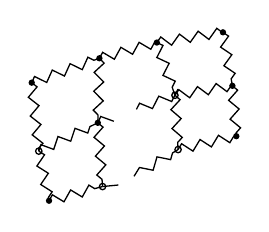
\begin{tikzpicture}[x=.010cm,y=-.010cm,line width=.47pt]
\coordinate (a) at (19,85);
\coordinate (b) at (105,54);
\coordinate (c) at (178,34);
\coordinate (d) at (262,21);
\coordinate (e) at (28,172);
\coordinate (f) at (103,136);
\coordinate (g) at (201,101);
\coordinate (h) at (274,89);
\coordinate (i) at (41,235);
\coordinate (j) at (109,217);
\coordinate (k) at (205,170);
\coordinate (l) at (279,153);
\foreach \from/\to in {a/b,b/c,c/d,a/e,b/f,c/g,d/h,e/f,g/h,e/i,f/j,g/k,h/l,i/j,k/l} {
  \draw[decorate,decoration={zigzag,amplitude=.62mm,segment length=2.4mm}] (\from)--(\to);
}
\draw[decorate,decoration={zigzag,amplitude=.60mm,segment length=2.6mm}]
  (f)--(127,126) (152,119)--(g) (j)--(128,209) (149,204)--(k);
\foreach \point in {a,b,c,d,f,h,i,l} \fill (\point) circle (1.15pt);
\foreach \point in {e,g,j,k} \draw (\point) circle (1.15pt);
\end{tikzpicture}}\endgroup\par
The gaps in the middle and lower rows are shown. The exact connections are unclear.}
\end{GelfandAdjacentEvidence}
\begin{GelfandAdjacentEvidence}{GELFAND-P001045}{9}

Connect the points with springs.

\uwave{A regular lattice} will not do:
\SourceFigure{GELFAND-P001045}{surface-outline}{%
\begingroup\color{black}\GelfandFitDiagram{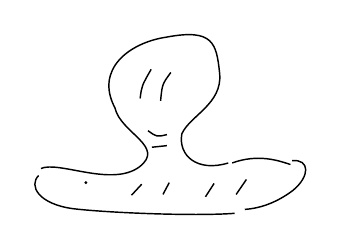
\begin{tikzpicture}[x=.010cm,y=-.010cm,line width=.52pt]
\draw (25,184) .. controls (48,174) and (115,208) .. (150,182)
 .. controls (184,156) and (126,139) .. (119,107)
 .. controls (93,58) and (137,24) .. (185,17)
 .. controls (244,6) and (248,25) .. (252,63)
 .. controls (256,102) and (214,117) .. (204,140)
 .. controls (199,168) and (224,189) .. (263,177);
\draw (268,177) .. controls (301,165) and (327,174) .. (342,179);
\draw (344,174) .. controls (367,172) and (367,194) .. (345,212)
 .. controls (321,230) and (299,235) .. (284,236);
\draw (271,241) .. controls (218,245) and (105,240) .. (65,235)
 .. controls (22,229) and (9,206) .. (22,193);
\draw (151,95)..controls (153,79)..(165,58);
\draw (177,98)..controls (179,77)..(190,62);
\draw (161,136)..controls (172,144)..(185,141);
\draw (166,157)--(185,155);
\draw (140,218)--(153,204) (180,217)--(188,202)
      (234,220)--(245,203) (273,217)--(286,198);
\fill (82,202) circle (.57pt);
\end{tikzpicture}}\endgroup\par
The drawing shows the visible gaps. The exact closure of the outline is unclear.}
\end{GelfandAdjacentEvidence}


For the lattice:
\begin{equation*}
\int\mathcal{D}\vec{x}(\xi^1,\xi^2)
e^{-\frac12\int\partial_a\vec{x}\cdot\partial^a\vec{x}\,d^2\xi}
\tag{26}
\end{equation*}
(for a two-dimensional surface in 26-dimensional space, one obtains the correct answer)

Suppose there is an intrinsic geometry described by $g_{ab}(\xi)$. The integral will take the form:


\Needspace{7\baselineskip}
\begin{GelfandAdjacentEvidence}{GELFAND-P001046}{1}
\SourcePage{GELFAND-P001046}{13}
\begin{equation*}
G=\int\mathcal D\vec{x}(\xi)
\exp\left\{-\frac12\int\sqrt{g}\,g^{ab}\partial_a\vec{x}\cdot\partial_b\vec{x}\,d^2\xi
+\lambda\int\sqrt{g}\,d^2\xi\right\}
\tag{27}
\end{equation*}
with the addition of $\lambda$, which we will choose.

Answer (correct):
\begin{equation*}
\begin{aligned}
G={}&\int\mathcal Dg_{ab}\int\mathcal D\vec{x}(\xi)\\
&\times\exp\left\{-\frac12\int\sqrt{g}\,g^{ab}\partial_a\vec{x}\,\partial_b\vec{x}\,d^2\xi
+\lambda\int\sqrt{g}\,d^2\xi\right\}
\end{aligned}
\tag{28}
\end{equation*}
\SourceFigure{GELFAND-P001046}{kinetic-dot}{A dot separates the derivatives in (27). In (28) they are juxtaposed.}
\end{GelfandAdjacentEvidence}
\begin{GelfandAdjacentEvidence}{GELFAND-P001046}{2}


By minimizing, we obtain the equations.

\medskip
\underline{4/$\overline{\underline{\mathrm{X}}}$-82 {}}\quad\underline{Gelfand Seminar.}

\underline{\uuline{Kirillov} on the work of Ginzburg}.

$G$ — a Lie group, $\mathfrak g$ — a Lie algebra, consider the orbits of the adjoint representation;

there are orbits in general position, and there are nilpotent ones (corresponding to nilpotent elements of the algebra $\mathfrak g$);

$\Omega_c$ — an orbit, $c=(c_1,\ldots,c_\ell)$ — its parameters ($\ell$ — the rank).

\underline{Example}: $SL(2,\mathbb R)$; $\mathfrak g\cong\mathbb R^3$; the orbits are \uwave{hyperboloids}.
\SourceFigure{GELFAND-P001046}{orbit-margin}{%
[At right \(\Vert\)] e.g., eigenvalues or,
\(\operatorname{Tr}A\), \(\operatorname{Tr}A^2,\ldots\)}
\end{GelfandAdjacentEvidence}
\begin{GelfandAdjacentEvidence}{GELFAND-P001046}{3}


\uwave{Desingularization according to Springer}.

$G$ — a semisimple group, $N\subset G$, $N$ — the set of unipotent elements
(with all eigenvalues $1$).

$N$ — an algebraic set with singularities.
\Unclear{GELFAND-P001046}{cancelled-before-osob}{A short entry before “singularities” is heavily crossed out. It may be “о.”}
\end{GelfandAdjacentEvidence}
\begin{GelfandAdjacentEvidence}{GELFAND-P001046}{4}


$B_0$ — a Borel subgroup in $G$; $\mathcal B$ — the collection of all Borel subgroups
(they are all conjugate), so that
\[
\mathcal B=\{gBg^{-1},\ g\in G\}.
\]
\SourceFigure{GELFAND-P001046}{borel-base-notation}{The formula has \(B\) without a subscript, while the preceding line has \(B_0\).}
\end{GelfandAdjacentEvidence}
\begin{GelfandAdjacentEvidence}{GELFAND-P001046}{5}


A desingularization of the algebraic set $X$ (with singularities) — a set $Y$ (without singularities)
of the same dimension, $Y\longrightarrow X$ is one-to-one almost everywhere
(except in smaller dimension).
\Unclear{GELFAND-P001046}{cancelled-definition-start}{The word before “Desingularization” is crossed out and may read “Всп.”.}
\end{GelfandAdjacentEvidence}
\begin{GelfandAdjacentEvidence}{GELFAND-P001046}{6}

\Unclear{GELFAND-P001046}{overwritten-toi}{The word corresponding to “same” is written over a correction. The earlier strokes are indistinct.}
\end{GelfandAdjacentEvidence}
\begin{GelfandAdjacentEvidence}{GELFAND-P001046}{7}


\underline{Example}:
\SourceFigure{GELFAND-P001046}{cylinder-cone}{%
\begingroup\color{black}\GelfandFitDiagram{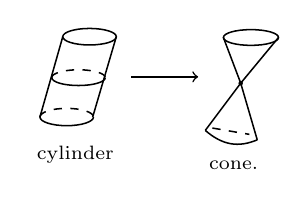
\begin{tikzpicture}[font=\scriptsize,line width=.55pt]
\draw (.20,.74) ellipse (.34 and .105);
\draw (-.14,.74)--(-.43,-.28) (.54,.74)--(.24,-.28);
\draw (-.28,.22) arc[start angle=180,end angle=360,x radius=.34,y radius=.10];
\draw[dashed] (-.28,.22) arc[start angle=180,end angle=0,x radius=.34,y radius=.10];
\draw (-.43,-.28) arc[start angle=180,end angle=360,x radius=.34,y radius=.11];
\draw[dashed] (-.43,-.28) arc[start angle=180,end angle=0,x radius=.34,y radius=.11];
\node at (.02,-.76) {cylinder};
\draw[->] (.73,.23)--(1.58,.23);
\draw (2.25,.73) ellipse (.35 and .10);
\draw (1.90,.73)--(2.12,.15)--(1.67,-.45) (2.60,.73)--(2.12,.15)--(2.33,-.57);
\fill (2.12,.15) circle (.82pt);
\draw (1.67,-.45) .. controls (1.89,-.64) and (2.09,-.67) .. (2.33,-.57);
\draw[dashed] (1.76,-.42)--(2.05,-.47)--(2.23,-.50);
\node at (2.03,-.89) {cone.};
\end{tikzpicture}}\endgroup}
\end{GelfandAdjacentEvidence}
\begin{GelfandAdjacentEvidence}{GELFAND-P001046}{8}

\[
(x,y,z)\longmapsto(xz,yz,z).
\]

\Unclear{GELFAND-P001046}{cancelled-incidence-name}{An indistinct symbol is crossed out after \(\mathcal M\).}
\end{GelfandAdjacentEvidence}
\begin{GelfandAdjacentEvidence}{GELFAND-P001046}{9}

\[
\mathcal M=\left\{\left(
\overset{\substack{N\\\rotatebox{-90}{\(\ni\)}}}{n},\,
\overset{\substack{\mathcal B\\\rotatebox{-90}{\(\ni\)}}}{B}
\right)\,\middle|\, n\in B\right\}\qquad\text{(flags).}
\]
\SourceFigure{GELFAND-P001046}{incidence-membership}{The membership signs above \(n\) and \(B\) are written vertically.}
\end{GelfandAdjacentEvidence}
\begin{GelfandAdjacentEvidence}{GELFAND-P001046}{10}

Then $\mathcal M$ — a desingularization of $N$.
\Unclear{GELFAND-P001046}{cancelled-before-m}{A symbol after “Then” is crossed out and illegible.}
\end{GelfandAdjacentEvidence}
\begin{GelfandAdjacentEvidence}{GELFAND-P001046}{11}


For $SL(2,\mathbb R)$ this is precisely what occurs in the example.

\underline{On Ginzburg again}.
\[
f\in C^\infty(\mathfrak g)\longmapsto\psi(c)=\int_{\Omega_c}f
\]
(the measure is chosen consistently on orbits in general position).
\[
\int_{\Omega_0}f=\left.P\psi(c)\right|_{c=0},
\qquad P\text{ — a differential operator}
\]
\SourceFigure{GELFAND-P001046}{orbital-operator}{The operator is written \(P\) in both places.}
\end{GelfandAdjacentEvidence}



\Needspace{7\baselineskip}
\begin{GelfandAdjacentEvidence}{GELFAND-P001047}{1}
\SourcePage{GELFAND-P001047}{unlabelled}
\underline{I. M. G.}\quad Integrals over hyperbolas are given. Find the value of the function at $0$.

(more generally — a hyperboloid).

\SourceFigure{GELFAND-P001047}{hyperbola-sketch}{%
\begingroup\color{black}\GelfandFitDiagram{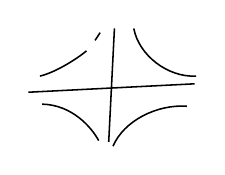
\begin{tikzpicture}[x=.91cm,y=.89cm,line width=.56pt]
\draw (-1.16,-.05)--(1.16,.07);
\draw (-.04,-.76)--(.04,.86);
\draw (-1.00,.18) .. controls (-.79,.23) and (-.49,.42) .. (-.35,.54);
\draw (-.23,.69)--(-.16,.80);
\draw (.31,.86) .. controls (.38,.48) and (.78,.16) .. (1.18,.18);
\draw (-.97,-.22) .. controls (-.55,-.23) and (-.28,-.55) .. (-.18,-.74);
\draw (.02,-.82) .. controls (.17,-.46) and (.63,-.22) .. (1.05,-.25);
\end{tikzpicture}}\endgroup\par
The short bend at the right end of the horizontal line is unclear.}
\end{GelfandAdjacentEvidence}
\begin{GelfandAdjacentEvidence}{GELFAND-P001047}{2}

\[
xy=c;\qquad\text{distance from }0\text{ of order }\sqrt c.
\]
For $|x|\geqslant1$ distance $\sim c$.
\Unclear{GELFAND-P001047}{upper-inequality}{The \(>\) sign has a separate slanted stroke beneath it. The intended sign is likely \(\geqslant\).}
\end{GelfandAdjacentEvidence}
\begin{GelfandAdjacentEvidence}{GELFAND-P001047}{3}


$\Rightarrow$ we evaluate the integral over the lines (limit of the integral over the hyperbolas) and so on.

See the expansion of $\delta(xy-c)$ in powers of $c$ in the first volume of Generalized Functions.

\medskip
\underline{Zamolodchikov.}

We want to find the sum
\begin{equation*}
\sum_S e^{-\mu_0^2 A(S)}
\tag{1}
\end{equation*}
$S$ — surface

The integral over the set of all curves (see above) had the form
\begin{equation*}
\begin{aligned}
\sum_P e^{-m_0L(P)}
&=\int_0^\infty d\tau\,e^{-m^2\tau}
\int_{\substack{\vec x(0)=\vec 0\\\vec x(\tau)=\vec R}}
\mathcal D\vec x(t)\,e^{-\frac12\int_0^\tau\dot{\vec x}^{\,2}(t)\,dt},\\
&\hspace{2em}L=\int\sqrt{\dot x^{2}}\,dt.
\end{aligned}
\tag{2}
\end{equation*}
\SourceFigure{GELFAND-P001047}{eq2-left-mass}{A subscript zero is visible between \(m\) and \(L\), touching the stroke of \(L\).}
\end{GelfandAdjacentEvidence}
\begin{GelfandAdjacentEvidence}{GELFAND-P001047}{4}

\SourceFigure{GELFAND-P001047}{length-notation}{In the formula for \(L\), \(\dot x\) has no arrow.}
\end{GelfandAdjacentEvidence}
\begin{GelfandAdjacentEvidence}{GELFAND-P001047}{5}


($m\ne m_0$ — renormalization)

And it is equal to:
\begin{equation*}
(\mathrm{const})\int_0^\infty d\tau
\left(e^{-m^2\tau-\frac{\vec R^{2}}{2\tau}}\right)\frac1{\tau^{d/2}},
\qquad d\text{ — dimension of the space}.
\tag{2'}
\end{equation*}
The relation between $m$ and $m_0$ depends on the method of regularization [approximation — fine structure of the space].

\begin{equation*}
\sum_P e^{-m_0L}=
\underset{\text{(integral)}}{\sum_{L=0}^{\infty}} f(L)e^{-m_0L}
\tag{3}
\end{equation*}
where
\[
f(L)\sim L^\beta e^{\varkappa L}
\qquad\text{when }L\gg\varepsilon
\qquad(\varepsilon\text{ — lattice spacing})
\]
\[
\varkappa=\varkappa(\varepsilon),\qquad\beta\text{ is independent of }\varepsilon.
\]
\Unclear{GELFAND-P001047}{growth-parameter}{The looped symbol is rendered as \(\varkappa\). A cursive \(x\) is also possible.}
\end{GelfandAdjacentEvidence}
\begin{GelfandAdjacentEvidence}{GELFAND-P001047}{6}


Hence
\begin{equation*}
(3)=\mathrm{const}\sum(L)^\beta e^{-(m_0-\varkappa)L}
\tag{4}
\end{equation*}
\[
m^2=m_0-\varkappa.
\]

\uwave{2 dangers}:

a) concentration on straight lines

b) it diverges

\SourceFigure{GELFAND-P001047}{risk-first-margin}{%
[At right of both items \(\Vert\)] are avoided by the choice of \(m_0\).}
\end{GelfandAdjacentEvidence}
\begin{GelfandAdjacentEvidence}{GELFAND-P001047}{7}

\SourceFigure{GELFAND-P001047}{risk-second-margin}{%
[Farther right \(\Vert\)] In an infinite-dimensional space almost any two measures are mutually singular.}
\end{GelfandAdjacentEvidence}



\Needspace{7\baselineskip}
\begin{GelfandAdjacentEvidence}{GELFAND-P001048}{1}
\SourcePage{GELFAND-P001048}{14}
\uwave{Let us pass to surfaces}.

$\vec{x}(\xi^1,\xi^2)$;\quad $g_{ab}(\xi^1,\xi^2)$ — the metric on the surface.

\begin{equation*}
\begin{aligned}
\sum_S e^{-\mu_0^2 A(S)}
={}&\int d\mu(\vec{x},g)\exp\Bigl\{-\frac12\int\sqrt{g}\,g^{ab}
\partial_a\vec{x}\,\partial_b\vec{x}\,d^2\xi{}-\\
&\qquad{}-\mu_{0}^{2}\int\sqrt{g}\,d^2\xi\Bigr\},
\qquad g=\det g_{ab}.
\end{aligned}
\tag{5}
\end{equation*}
\Unclear{GELFAND-P001048}{eq5-mu-subscript}{The subscript of the second \(\mu\) is heavily overwritten. It is probably \(0\).}
\end{GelfandAdjacentEvidence}
\begin{GelfandAdjacentEvidence}{GELFAND-P001048}{2}


(Polyakov formula) Here we sum over surfaces [inserted above: with] given topological properties.
\SourceFigure{GELFAND-P001048}{top-preposition-insertion}{The preposition “с” (“with”) is inserted between “surfaces” and “given.”}
\end{GelfandAdjacentEvidence}
\begin{GelfandAdjacentEvidence}{GELFAND-P001048}{3}


\[
\left[
\begin{minipage}{.87\linewidth}
In fact one has to take account of surfaces with handles and holes.

It is unclear how the contributions compare.\quad One needs: $\displaystyle\sum$, $j$ — the number of handles.

Foamy surfaces (with many handles) can make an overwhelming contribution.
\end{minipage}
\right.
\]
\Unclear{GELFAND-P001048}{handles-sum-index}{A small mark is visible under \(\sum\), without a discernible \(j\) there. The text to the right calls \(j\) the number of handles.}
\end{GelfandAdjacentEvidence}
\begin{GelfandAdjacentEvidence}{GELFAND-P001048}{4}


Here we choose a parameter domain in $\mathbb R^2$.
One introduces [inserted above: elements of] distance in the function space:
\SourceFigure{GELFAND-P001048}{distance-verb}{The start of the phrase reads “Вводятся” (“are introduced”).}
\end{GelfandAdjacentEvidence}
\begin{GelfandAdjacentEvidence}{GELFAND-P001048}{5}

\SourceFigure{GELFAND-P001048}{distance-insertion}{The word “elements” is written above the line.}
\end{GelfandAdjacentEvidence}
\begin{GelfandAdjacentEvidence}{GELFAND-P001048}{6}

\SourceFigure{GELFAND-P001048}{distance-noun}{The word “расстояния” (“distance” or “distances”) is written on the line.}
\end{GelfandAdjacentEvidence}
\begin{GelfandAdjacentEvidence}{GELFAND-P001048}{7}

\begin{equation*}
\begin{aligned}
\|\delta\vec{x}(\xi^1,\xi^2)\|^2
&=\int\sqrt{g}\,(\delta\vec{x}(\xi))^2\,d^2\xi\\
\|\delta g\|^2
&=\int\sqrt{g}\,
\bigl(g^{aa'}g^{bb'}+c\,g^{ab}g^{a'b'}\bigr)
\delta g_{ab}\,\delta g_{a'b'}\,d^2\xi
\end{aligned}
\tag{6}
\end{equation*}
Gauge invariance under the transformations:
\begin{equation*}
\begin{cases}
\xi^a\to\xi^a+\varepsilon^a(\xi),\\
g_{ab}\to g_{ab}+\nabla_a\varepsilon_b+\nabla_b\varepsilon_a,
\end{cases}
\qquad
\nabla_a\varepsilon_b=\partial_a\varepsilon_b+\Gamma_{ab}^{c}\varepsilon_c.
\tag{7}
\end{equation*}
nothing changes.
\SourceFigure{GELFAND-P001048}{covariant-derivative-sign}{A \(+\) appears before \(\Gamma_{ab}^{c}\) in (7).}
\end{GelfandAdjacentEvidence}
\begin{GelfandAdjacentEvidence}{GELFAND-P001048}{8}


One must integrate over the \uuline{space of orbits}.
\begin{equation*}
d\mu(x,g)=\frac{\mathcal{D}\vec{x}\,\mathcal{D}g}{\mathcal{D}\omega}
\tag{8}
\end{equation*}
\begin{equation*}
\|\varepsilon\|^2=\int\sqrt{g}\,g^{ab}\varepsilon_a\varepsilon_b\,d^2\xi
\tag{9}
\end{equation*}
\SourceFigure{GELFAND-P001048}{measure-margin}{%
[At right of (8) and (9)] \(\mathcal D\omega\) — the measure on the group one quotients by,\\
\(\mathcal D\vec{x}\) and \(\mathcal D g\) are introduced using the metrics \underline{(6)}\\
\(\mathcal D\omega\) — using the metric (9) on the Lie algebra.}
\end{GelfandAdjacentEvidence}
\begin{GelfandAdjacentEvidence}{GELFAND-P001048}{9}


Now the integral [inserted above: (5)] is well defined.
\SourceFigure{GELFAND-P001048}{eq5-number-insertion}{The reference “(5)” is inserted above the line.}
\end{GelfandAdjacentEvidence}
\begin{GelfandAdjacentEvidence}{GELFAND-P001048}{10}


$\int\mathcal{D}\vec{x}$ is Gaussian and reduces to the $\underline{\det}$ of the operator.

Polyakov proposes choosing representatives as follows:
\begin{equation*}
g_{ab}=\delta_{ab}\,\rho(\xi^1,\xi^2)
\qquad\text{(conformally flat form).}
\tag{10}
\end{equation*}
(choice of gauge). The conformal group remains (finite-dimensional).
\SourceFigure{GELFAND-P001048}{conformal-group-adjective}{The opening strokes of “finite-dimensional” have been overwritten.}
\end{GelfandAdjacentEvidence}


$\det$ are the same. One obtains
\begin{equation*}
\int d\mu(\rho)\,[\det(\Delta_g)]^{(26-d)/2},
\qquad\Delta_g\text{ — Laplacian of the metric}
\tag{11}
\end{equation*}
($\rho$ — the coefficient in (10)).


\Needspace{7\baselineskip}
\begin{GelfandAdjacentEvidence}{GELFAND-P001049}{1}
\SourcePage{GELFAND-P001049}{unlabelled}
One obtains:
\begin{equation*}
(11)=\int d\mu(\varphi)\,
e^{\frac{d-26}{48\pi}\int\frac12(\partial_a\varphi)^2+
m^{2}e^{\varphi})\,d^2\xi}
\tag{12}
\end{equation*}
\SourceFigure{GELFAND-P001049}{eq11-crossreference}{The reference “(11)” to the left of the equals sign is written over earlier strokes.}
\end{GelfandAdjacentEvidence}
\begin{GelfandAdjacentEvidence}{GELFAND-P001049}{2}

\Unclear{GELFAND-P001049}{eq12-mass-symbol}{The base of the power before \(e^\varphi\) is heavily overwritten and reads as \(m\). The earlier strokes are indistinct.}
\end{GelfandAdjacentEvidence}
\begin{GelfandAdjacentEvidence}{GELFAND-P001049}{3}

\Unclear{GELFAND-P001049}{eq12-parentheses}{A closing parenthesis follows \(e^\varphi\). An opening parenthesis for the whole sum is indistinct.}
\end{GelfandAdjacentEvidence}


$d\mu(\varphi)$ — the measure from the metric
\begin{equation*}
\|\delta\varphi\|^2=\int e^{\varphi}(\delta\varphi)^2\,d^2\xi
\tag{13}
\end{equation*}


\Needspace{7\baselineskip}
\begin{GelfandAdjacentEvidence}{GELFAND-P001050}{1}
\SourcePage{GELFAND-P001050}{unlabelled}
\underline{11/$\overline{\underline{\mathrm{X}}}$-82 {}}\qquad
\uwave{Gelfand Seminar}

\uuline{V. Ginzburg.}

\underline{after Guillemin–Sternberg} (on integral geometry)
\SourceFigure{GELFAND-P001050}{guillemin-sternberg-heading}{The right-hand heading reads “after Guillemin–Sternberg.”}
\end{GelfandAdjacentEvidence}
\begin{GelfandAdjacentEvidence}{GELFAND-P001050}{2}


$X$ — a set (complex)

$\Sigma\subset T^*X$, $\Sigma$ — a coisotropic subset,
\Unclear{GELFAND-P001050}{crossed-after-submanifold}{The word after “subset” is crossed out and may read “which” or “conic.”}
\end{GelfandAdjacentEvidence}
\begin{GelfandAdjacentEvidence}{GELFAND-P001050}{3}

has the following properties:

1.\quad $\Sigma$ — is conic;

2.\quad $\Sigma\to X$ is a fibration.

On $\Sigma$ there is a $0$-foliation (kernel of the symplectic form), which is always \uwave{integrable}.

Locally arranged as follows: $q_1,\ldots,q_n,p_1,\ldots,p_k$

$0$-foliation
\SourceFigure{GELFAND-P001050}{null-foliation-bracket}{%
\begingroup\color{black}\GelfandFitDiagram{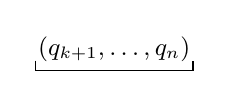
\begin{tikzpicture}[font=\small,line width=.45pt]
\node (coords) at (0,0) {$(q_{k+1},\ldots,q_n)$};
\draw (coords.south west) ++(.09,.14) -- ++(0,-.13)
  -- ([xshift=-.09cm,yshift=.01cm]coords.south east) -- ++(0,.13);
\end{tikzpicture}}\endgroup}
\end{GelfandAdjacentEvidence}
\begin{GelfandAdjacentEvidence}{GELFAND-P001050}{4}


\Unclear{GELFAND-P001050}{mark-before-pust}{There is a mark before “Suppose,” possibly “Мы” (“we”) or “Или” (“or”).}
\end{GelfandAdjacentEvidence}
\begin{GelfandAdjacentEvidence}{GELFAND-P001050}{5}

Suppose it is a \uwave{fibration} (all leaves are closed, etc.)
\SourceFigure{GELFAND-P001050}{quotient-arrow}{%
\begingroup\color{black}\GelfandFitDiagram{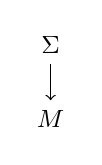
\begin{tikzpicture}[font=\small,line width=.47pt]
\node (from) at (0,.45) {$\Sigma$};
\node (to) at (0,-.48) {$M$};
\draw[->] (from.south)--(to.north);
\end{tikzpicture}}\endgroup}
\end{GelfandAdjacentEvidence}

and $M$ — the quotient space.

From $\Sigma$ construct a Lagrangian subset $\Lambda\subset T^*X\times T^*X$:
\[
\Lambda=\{(\xi_1,\xi_2):\quad\xi_1,\xi_2\in\Sigma,\quad\xi_1\sim\xi_2\}
\]
\underline{Properties}:

1)\quad $\Lambda^t=\Lambda$

2)\quad $\Lambda\circ\Lambda=\Lambda$ \qquad (projector)


\Needspace{7\baselineskip}
\begin{GelfandAdjacentEvidence}{GELFAND-P001051}{1}
\SourcePage{GELFAND-P001051}{unlabelled}
Apparently the converse: if $\Lambda$ is Lagrangian and satisfies 1), 2), then it is obtained from $\Sigma$.
\Unclear{GELFAND-P001051}{top-cancel-01}{A word after “and” is heavily crossed out. A loop is visible beneath the cancellation.}
\end{GelfandAdjacentEvidence}
\begin{GelfandAdjacentEvidence}{GELFAND-P001051}{2}


Fourier integral operators are constructed from $\Lambda$: denote their set by $\mathcal E_\Lambda$.

It is a ring by property 2).
\Unclear{GELFAND-P001051}{top-cancel-02}{A short entry before “property” is crossed out.}
\end{GelfandAdjacentEvidence}
\begin{GelfandAdjacentEvidence}{GELFAND-P001051}{3}


This is an analogue of the Radon transform.

$X=X_1\times X_2$;\quad $\Sigma$ — directions normal to $X_1$ (along $X_2$)
in the cotangent bundle.
\[
\begin{aligned}
\Lambda
&=\operatorname{diag}(T^*X_1\times T^*X_1)\times 0\\
&\subset T^*X_1\times T^*X_1\times T^*X_2\times T^*X_2.
\end{aligned}
\]
\Unclear{GELFAND-P001051}{lambda-cancel}{A formula before \(\operatorname{diag}\) is crossed out. Individual signs resembling \(T^*\), \(X_1\), \(\times\), and \(0\) are visible.}
\end{GelfandAdjacentEvidence}
\begin{GelfandAdjacentEvidence}{GELFAND-P001051}{4}


\dashuline{Operators}:\quad in $X_1$ all pseudodifferential.

\hspace{5em}in $X_2$ smoothing.

\uuline{Shmelyov.}
\SourceFigure{GELFAND-P001051}{speaker-name}{The twice-underlined surname reads “Shmelyov.”}
\end{GelfandAdjacentEvidence}
\begin{GelfandAdjacentEvidence}{GELFAND-P001051}{5}

\SourceFigure{GELFAND-P001051}{double-fibration}{%
\begingroup\color{black}\GelfandFitDiagram{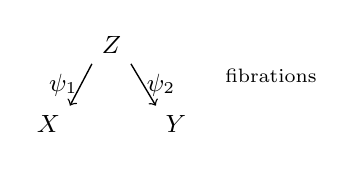
\begin{tikzpicture}[font=\small,line width=.50pt]
\node (z) at (0,.49) {$Z$};
\node (x) at (-.80,-.51) {$X$};
\node (y) at (.82,-.51) {$Y$};
\draw[->] (z.south west)--node[left,inner sep=1pt] {$\psi_1$} (x.north east);
\draw[->] (z.south east)--node[right,inner sep=1pt] {$\psi_2$} (y.north west);
\node[anchor=west,font=\scriptsize] at (1.32,.11) {fibrations};
\end{tikzpicture}}\endgroup}
\end{GelfandAdjacentEvidence}
\begin{GelfandAdjacentEvidence}{GELFAND-P001051}{6}


Requirement:\quad
\uwave{\(\psi_2^*:N^*Z\longrightarrow T^*Y\)}
\quad an embedding;

\underline{Fröhlich}

1) Magnetic monopoles

2) Gauge theories\quad $G\overset{\text{e.g.}}{=}SU(2)$

Lagrangian:\quad $\varphi:\ \mathrm{isospin}=1$ \quad (3 components)
\begin{equation*}
\begin{aligned}
E
&=\int\{(D_A\varphi)^2+F^2\}\\
&=\int\Bigl\{
\bigl|(\partial_\mu-eA_\mu\wedge)\varphi(x)\bigr|^2
+\operatorname{tr}(F_{\mu\nu}\cdot F^{\mu\nu})(x)
\Bigr\}\,dx,
\end{aligned}
\tag{1}
\end{equation*}
\SourceFigure{GELFAND-P001051}{energy-wedge}{A sign resembling \(\wedge\) follows \(A_\mu\).}
\end{GelfandAdjacentEvidence}
\begin{GelfandAdjacentEvidence}{GELFAND-P001051}{7}

\Unclear{GELFAND-P001051}{energy-norm-cancel}{A mark beneath the squared norm is heavily crossed out.}
\end{GelfandAdjacentEvidence}
\begin{GelfandAdjacentEvidence}{GELFAND-P001051}{8}

\Unclear{GELFAND-P001051}{energy-trace-cancel}{Below the dot between the two \(F\)s are overwritten strokes and a wavy line. The earlier marks are indistinct.}
\end{GelfandAdjacentEvidence}
\begin{GelfandAdjacentEvidence}{GELFAND-P001051}{9}


$x\in\mathbb R^3$
\Unclear{GELFAND-P001051}{energy-line-cancel}{An equality to the right of \(x\in\mathbb R^3\) is crossed out. It appears to begin \(E=E\).}
\end{GelfandAdjacentEvidence}
\begin{GelfandAdjacentEvidence}{GELFAND-P001051}{10}

\[
F_{\mu\nu}=\partial_\mu A_\nu-\partial_\nu A_\mu+[A_\mu,A_\nu].
\]

Monopole:\quad a solution of the Euler–Lagrange equations such that the degree of $\varphi|_{S^2}\longrightarrow S^2$
at \(\infty\) equals 1.\quad \(\Vert\) (stationary solutions)

$\exists$ solutions attaining $\min$ or $\text{loc.}\,\min$ — explicitly, using twistor techniques.
\Unclear{GELFAND-P001051}{twistor-cancel}{A short entry before “twistor” is crossed out.}
\end{GelfandAdjacentEvidence}
\begin{GelfandAdjacentEvidence}{GELFAND-P001051}{11}


Question:\quad other stationary points?

\uwave{Answer}:\quad solutions have been found that are not minima

\underline{Idea}:
\SourceFigure{GELFAND-P001051}{lower-loop-diagram}{%
\begingroup\color{black}\GelfandFitDiagram{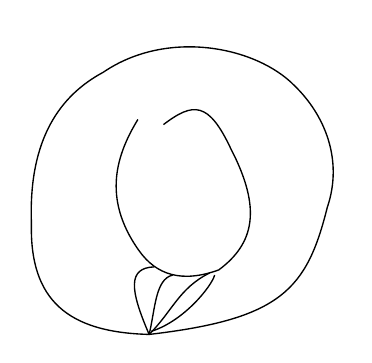
\begin{tikzpicture}[x=.013cm,y=-.013cm,line width=.49pt]
\draw (123,307) .. controls (44,305) and (6,274) .. (8,198)
 .. controls (5,115) and (37,73) .. (78,51)
 .. controls (141,8) and (228,26) .. (265,64)
 .. controls (294,92) and (313,136) .. (297,183)
 .. controls (277,263) and (252,292) .. (123,307);
\draw (137,102) .. controls (166,80) and (181,79) .. (203,126)
 .. controls (233,184) and (226,218) .. (191,244)
 .. controls (155,257) and (130,249) .. (113,225)
 .. controls (76,173) and (92,130) .. (112,97);
\draw (123,307) .. controls (104,263) and (102,242) .. (128,241);
\draw (123,307) .. controls (129,282) and (129,253) .. (146,249);
\draw (123,307) .. controls (146,284) and (152,262) .. (182,247);
\draw (125,304) .. controls (157,294) and (184,260) .. (187,249);
\end{tikzpicture}}\endgroup\par
The inner loop has a gap. The exact connections of the thin lines at the bottom are indistinct.}
\end{GelfandAdjacentEvidence}
\begin{GelfandAdjacentEvidence}{GELFAND-P001051}{12}


one-parameter family:
\[
\max_{[\rho?]\,t\in\mathrm{curve}}\ \min_{\mathrm{curve.}}(\varphi_t,F_t)
\]
\Unclear{GELFAND-P001051}{minimax-index}{Before \(t\in\mathrm{curve}\) is a sign resembling \(\rho\) or \(p\). Below \(\min\) the manuscript has “curve.”.}
\end{GelfandAdjacentEvidence}


C. Taubes

The new solution resembles a pair

monopole / antimonopole.


\Needspace{7\baselineskip}
\begin{GelfandAdjacentEvidence}{GELFAND-P001052}{1}
\SourcePage{GELFAND-P001052}{16}
\uwave{There is a manifold}\quad
$\underset{\text{(compact)}}{M^4}$,
$\pi_1(M^4)=\{\mathrm{id}\}$;
$H^2(M^4)=\{0\}$.

$M^4$ with a conformal structure.

$\exists\, [A_\mu?]$ a solution of the equation $F=\pm F^*$?
\Unclear{GELFAND-P001052}{top-field-symbol}{The symbol after \(\exists\) is overwritten and may be \(A_\mu\).}
\end{GelfandAdjacentEvidence}
\begin{GelfandAdjacentEvidence}{GELFAND-P001052}{2}


$*$ — Hodge duality;

with characteristic class 1 — \uwave{[e.g.?]}
\Unclear{GELFAND-P001052}{top-underlined-name}{The underlined word after “class 1” may read “напр.” (“e.g.”). Its opening has been overwritten.}
\end{GelfandAdjacentEvidence}
\begin{GelfandAdjacentEvidence}{GELFAND-P001052}{3}


$F$ is the curvature of the connection $A$; the group — $SU(2)$.

Answer:\quad a solution exists!

Space of parameters labelling solutions
$\displaystyle=\underset{\substack{\nwarrow\\\text{manifold }B}}{5}$
\qquad (as on the sphere!)

(Taubes, Comm. Math. Phys, 1981).

Instanton parameters

$B$ — a manifold with boundary,
$\displaystyle\partial B\underset{\substack{\uparrow\\\text{\uwave{Donaldson}}}}{\simeq}M^4$
\quad (the original manifold)
\SourceFigure{GELFAND-P001052}{boundary-annotation}{The name “Donaldson” is connected to \(\simeq\) by an angled arrow.}
\end{GelfandAdjacentEvidence}
\begin{GelfandAdjacentEvidence}{GELFAND-P001052}{4}


\begin{align*}
M^4\text{ — a boundary}
&\Longleftrightarrow(\text{Pontr. }\text{[?]}\ \text{class}=0)\\
&\Longleftrightarrow(\text{signature}=0\text{ for the form in }H^2).
\end{align*}
\Unclear{GELFAND-P001052}{pontryagin-symbol}{A sign between “Pontr.” and “class” is heavily overwritten. It may be \(p\).}
\end{GelfandAdjacentEvidence}
\begin{GelfandAdjacentEvidence}{GELFAND-P001052}{5}


\uwave{Donaldson}: if the form on $H^2$ is positive definite, then the manifold $=$
generalized projective plane $CP^2$
$\Rightarrow$ the form reduces to a sum of squares (over $\mathbb Z$).
\Unclear{GELFAND-P001052}{definite-cancel}{A short entry between “positive” and “definite” is crossed out.}
\end{GelfandAdjacentEvidence}
\begin{GelfandAdjacentEvidence}{GELFAND-P001052}{6}

\Unclear{GELFAND-P001052}{manifold-cancel}{The word immediately after the equals sign is crossed out.}
\end{GelfandAdjacentEvidence}
\begin{GelfandAdjacentEvidence}{GELFAND-P001052}{7}

\Unclear{GELFAND-P001052}{projective-correction}{An entry after “projective” is crossed out. “Plane” is added above and \(CP^2\) below. Both additions are outlined.}
\end{GelfandAdjacentEvidence}
\begin{GelfandAdjacentEvidence}{GELFAND-P001052}{8}


$B$ must have singularities — cones over $CP^2$.

\underline{On the work of} \uwave{Witten}.

$M$ — $n$-dimensional manifold, $B_p$ — the \(p\)th Betti number.

$f$ — a function on $M$ with isolated critical points.

$M_p$ — the number of critical points of index $p$ (the Hessian has $p$ negative eigenvalues).
\[
M_p\geqslant B_p
\qquad\underset{\text{the simplest one}}{\text{(Morse inequality)}}
\]

$d:\Omega_p\longrightarrow\Omega_{p+1}$ (exterior differential)
\Unclear{GELFAND-P001052}{differential-cancel}{A mark before “exterior differential” is crossed out.}
\end{GelfandAdjacentEvidence}
\begin{GelfandAdjacentEvidence}{GELFAND-P001052}{9}


Introduce a metric on $M$; $*$ — the corresponding operator.

Choose in $H^p$ a basis of harmonic $p$-forms ($B_p$ in number)

\uwave{Alternatively}: set
\[
d_t=e^{-tf}d\,e^{tf}
\]
\SourceFigure{GELFAND-P001052}{omega-exponent}{%
\begingroup\color{black}\GelfandFitDiagram{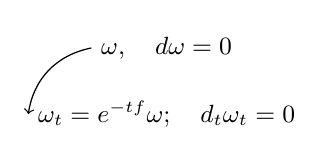
\begin{tikzpicture}[font=\small,line width=.45pt]
\node (top) at (0,.40) {$\omega,\quad d\omega=0$};
\node (bottom) at (0,-.44) {$\omega_t=e^{-tf}\omega;\quad d_t\omega_t=0$};
\draw[->] (top.west) to[bend right=35] (bottom.west);
\end{tikzpicture}}\endgroup\par
The exponent of \(e\) has been overwritten and reads as \(-tf\).}
\end{GelfandAdjacentEvidence}
\begin{GelfandAdjacentEvidence}{GELFAND-P001052}{10}


Choose a basis in $H^p$, satisfying the conditions:
\begin{equation*}
\left\{
\begin{aligned}
-d_t\omega_j&=0\\
-(\omega_j,d_t\beta)&=0,\quad\forall\beta\in\Omega_{p-1}
\end{aligned}
\right\}
\ \Rightarrow\
(d_t^*d_t+d_t d_t^*)\omega_j=0
\tag{1}
\end{equation*}
\begin{flushright}(closed in the new sense).\end{flushright}
\Unclear{GELFAND-P001052}{harmonic-first-stroke}{The short stroke before \(d_t\omega_j\) may be a minus or an item dash.}
\end{GelfandAdjacentEvidence}
\begin{GelfandAdjacentEvidence}{GELFAND-P001052}{11}

\Unclear{GELFAND-P001052}{harmonic-second-stroke}{A separate horizontal stroke also precedes the second line.}
\end{GelfandAdjacentEvidence}



\Needspace{7\baselineskip}
\begin{GelfandAdjacentEvidence}{GELFAND-P001053}{1}
\SourcePage{GELFAND-P001053}{unlabelled}
$d_t$-cohomology is the same as $d$-cohomology, since there is a \uwave{homotopy}.
\[
d_t^2=0\quad\text{(obvious)}
\]
Let us compute the operator $\Box_t=d_t^*d_t+d_td_t^*$ and find its asymptotics
as $t\to\infty$.
\SourceFigure{GELFAND-P001053}{operator-word}{The manuscript reads “Let us compute the operator.” A diagonal stroke is visible inside the box sign.}
\end{GelfandAdjacentEvidence}
\begin{GelfandAdjacentEvidence}{GELFAND-P001053}{2}

\begin{equation*}
\begin{cases}
d_t=d-tdf\cdot a^*,\\
d_t^*=d^*-tdf\cdot a
\end{cases}
\qquad
\begin{gathered}
df\,a^*\omega\equiv df\wedge\omega\\
\text{(physics notation)}
\end{gathered}
\tag{2}
\end{equation*}
\SourceFigure{GELFAND-P001053}{eq2-sign-consistency}{Both \(tdf\) terms in (2) carry minus signs.}
\end{GelfandAdjacentEvidence}
\begin{GelfandAdjacentEvidence}{GELFAND-P001053}{3}

\begin{equation*}
\{a_j,a_i^*\}=\delta_{ij}.
\tag{3}
\end{equation*}
$a_i$ — \sout{basis} correspond to the basis of 1-forms;
(operators of exterior multiplication).
\SourceFigure{GELFAND-P001053}{basis-cancellation}{After \(a_i\), “basis” is crossed out.}
\end{GelfandAdjacentEvidence}
\begin{GelfandAdjacentEvidence}{GELFAND-P001053}{4}


Choose so that one has (3).
\Unclear{GELFAND-P001053}{middle-operators}{The entry before “one has” is heavily crossed out. It may contain \(a_i\).}
\end{GelfandAdjacentEvidence}
\begin{GelfandAdjacentEvidence}{GELFAND-P001053}{5}


\underline{Kirillov}:
\[
a=(a^1,a^2,\ldots,a^n)\text{ — \uwave{a vector}},\qquad
df=(\partial_1f,\partial_2f,\ldots,\partial_nf)
\]
$a^i$ — interior multiplication (annihilation operator) — strike out $dx^i$, where it occurs,
where it does not occur, annihilate.
\Unclear{GELFAND-P001053}{middle-cancellation}{A word before “annihilation” is crossed out. It may be an abbreviation for “creation.”}
\end{GelfandAdjacentEvidence}
\begin{GelfandAdjacentEvidence}{GELFAND-P001053}{6}


$a^{i*}$ — exterior multiplication.

Indices can be lowered and raised using the metric.

$a^j$ — interior multiplication by $\dfrac{\partial}{\partial x^j}$ (substitution in the first argument)

$df\cdot a$ — interior multiplication by the field obtained from $df$ by raising the index
\[
a_i^*=dx_i\wedge\qquad\text{(exterior multiplication)}
\]
\underline{Fröhlich.}
\[
a_i=\partial/\partial x_i\,
\tikz[baseline=0pt,x=1em,y=1em]{\draw (0,.62)--(0,0)--(.68,0);}
\qquad\text{(interior multiplication)}
\]
\SourceFigure{GELFAND-P001053}{contraction-corner}{An angle-shaped sign follows \(\partial/\partial x_i\).}
\end{GelfandAdjacentEvidence}
\begin{GelfandAdjacentEvidence}{GELFAND-P001053}{7}

Meaning:

One-particle space (fermions)
\[
\{1,2,\ldots,n\}\to\ell_2(\{1,2,\ldots,n\}).
\]
($\ell_2$ on a finite set).
\[
m\text{ particles (fermions)}\Rightarrow f_{i_1\ldots i_m}
\]
(antisymmetric $\delta$-functions — basis)

A way of writing elements of the Grassmann algebra.

(see Berezin: The Method of Second Quantization)
\begin{equation*}
\sum_{i_1\ldots i_m}a_{i_1}^*\ldots a_{i_m}^*f_{i_1\ldots i_m}\Omega_0
\tag{4}
\end{equation*}
\[
\begin{gathered}
\updownarrow\\
(f_{i_1}\ldots f_{i_m})\quad\text{(list of coefficients)}
\end{gathered}
\]
\Unclear{GELFAND-P001053}{lower-coefficients}{The last base is overwritten and may read \(f_{i_m}\) or \(h_{i_m}\).}
\end{GelfandAdjacentEvidence}



\Needspace{7\baselineskip}
\begin{GelfandAdjacentEvidence}{GELFAND-P001054}{1}
\SourcePage{GELFAND-P001054}{17}
It is postulated:
\begin{equation*}
\{a_i,a_j^*\}=\delta_{ij}
\tag{5}
\end{equation*}
Exterior multiplication by $df$ — a fermion creation operator.
\begin{equation*}
a_i\Omega_0=0,\quad\forall i
\tag{6}
\end{equation*}
\begin{equation*}
\Box_t=\Box+t^2(df)^2+t\sum[a_i^*,a_j]\partial_i\partial_jf
\tag{7}
\end{equation*}
In a neighborhood of the critical point
\begin{equation*}
f(x)=\sum_{i=1}^{n-p}\lambda_i(x^i-x_0^i)^2
-\sum_{j=n-p+1}^{n}\lambda_j(x^j-x_0^j)^2
+O(|x-x_0|^3)
\tag{8}
\end{equation*}
\begin{center}— . —\end{center}

\underline{I. M. G.}\quad Idea: instead of changes in cycles — \uwave{changes in forms}!

Connection between PDOs and \dashuline{Morse changes}.

F.\quad\uwave{the principal term of} $\Box_t$ \uwave{equals}:
\begin{equation*}
\Box+4t^2\sum_{j=1}^{n}\lambda_j^2(x^j-x_0^j)^2+
\overbrace{t\sum_{i<j}[a_i^*,a_j]\underset{\text{const}}{c_{ij}}}
\tag{9}
\end{equation*}
[Above the last term]
\[
-4t\sum_{1}^{n-p}[a_i,a_i^*]\lambda_i
+4t\sum_{n-p+1}^{n}\lambda_i[\,].
\]
\SourceFigure{GELFAND-P001054}{expansion-above-nine}{The square brackets in the second sum are empty.}
\end{GelfandAdjacentEvidence}
\begin{GelfandAdjacentEvidence}{GELFAND-P001054}{2}

\Unclear{GELFAND-P001054}{middle-margin-cancellation}{A short word above the bracket is crossed out, possibly “sign.” Two slanted strokes follow.}
\end{GelfandAdjacentEvidence}
\begin{GelfandAdjacentEvidence}{GELFAND-P001054}{3}

\SourceFigure{GELFAND-P001054}{eq9-summation-index}{The index beneath the sum in (9) reads \(i<j\).}
\end{GelfandAdjacentEvidence}
\begin{GelfandAdjacentEvidence}{GELFAND-P001054}{4}

\begin{equation*}
\bigm|\ \approx\quad\uwave{Annihilates}:\quad
\underline{dx_{n-p+1}\wedge\cdots\wedge dx_n}\quad(p\text{-form})
\tag{10}
\end{equation*}
\SourceFigure{GELFAND-P001054}{annihilation-form}{A lower bracket surrounds the \(p\)-form.}
\end{GelfandAdjacentEvidence}
\begin{GelfandAdjacentEvidence}{GELFAND-P001054}{5}

Let us look at eigenvalues other than the $0$-th, the small ones.
\SourceFigure{GELFAND-P001054}{eigenvalue-word}{The manuscript reads “small eigenvalues.”}
\end{GelfandAdjacentEvidence}
\begin{GelfandAdjacentEvidence}{GELFAND-P001054}{6}


$\forall$ critical point gives an approximation to an eigenfunction.

The second [inserted above: term]
cancels the 1-st exactly on the first vector (10).
\Unclear{GELFAND-P001054}{middle-second-term}{After “second,” a word, possibly “vector,” is crossed out and “term” is inserted.}
\end{GelfandAdjacentEvidence}
\begin{GelfandAdjacentEvidence}{GELFAND-P001054}{7}


The cancellation follows from supersymmetry considerations.

$d_t$ plays the role of a supercharge; Yukawa model — the cancellation is known.
\begin{equation*}
a=\frac{\delta}{\delta\varphi(x)}+ta^*(x)\varphi^n(x)
\leftrightarrow d+tdf\cdot a^*
\tag{11}
\end{equation*}
\SourceFigure{GELFAND-P001054}{eq11-field-power}{In (11) the exponent of \(\varphi\) is \(n\).}
\end{GelfandAdjacentEvidence}


\underline{$d=2$}$\Rightarrow$ fermions $=$ forms on the set of Bose-field configurations.

(since the Poincaré group is simple)

\underline{$d>2$}$\Rightarrow$ (?) gauge fields are needed for the interpretation. —

— there is no (such) interpretation yet.

\underline{V. Enss} — asymptotic completeness of systems of particles with Coulomb interactions.

(three-particle)\qquad (worked on it for 15 years)

— a classical problem of mathematical physics.


\Needspace{7\baselineskip}
\begin{GelfandAdjacentEvidence}{GELFAND-P001055}{1}
\SourcePage{GELFAND-P001055}{unlabelled}
\uuline{18/$\overline{\underline{\mathrm X}}$-82 {}}\qquad
\underline{Gelfand Seminar}

\uwave{Fröhlich}.\qquad\underline{Statistical mechanics of surfaces}.

Arises in the following settings:
\Unclear{GELFAND-P001055}{heading-cancellation}{A short entry after “в” (“in”) is crossed out and may read “во.”}
\end{GelfandAdjacentEvidence}
\begin{GelfandAdjacentEvidence}{GELFAND-P001055}{2}


(a)\quad Crystal growth

(b)\quad Interfaces separating different phases

(c)\quad (lattice) gauge theories

(d)\quad dual resonance models (strings)

Simplified model for (a), (b):
\begin{equation*}
\underset{\substack{\vert\\\text{finite subset}}}{\Lambda}\subset\mathbb Z^2;
\qquad
h:p\subset\mathbb Z^2\to h_p\in\mathbb Z.
\tag{1}
\end{equation*}
\SourceFigure{GELFAND-P001055}{mapping-domain-notation}{The symbol following \(p\) is \(\subset\).}
\end{GelfandAdjacentEvidence}
\begin{GelfandAdjacentEvidence}{GELFAND-P001055}{3}

(solid-on-solid model)

\SourceFigure{GELFAND-P001055}{surface-lattice}{%
\begingroup\color{black}\GelfandFitDiagram{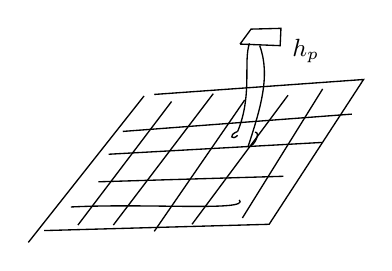
\begin{tikzpicture}[x=.010cm,y=-.010cm,font=\small,line width=.48pt]
\draw (6,303)--(153,117) (166,115)--(432,96)--(312,280)--(26,288);
\draw (69,281)--(188,124)
      (114,281)--(241,114)
      (166,289)--(281,122)
      (214,280)--(336,116)
      (278,272)--(380,108);
\draw (126,162)--(417,140)
      (108,191)--(379,176)
      (95,226)--(330,219)
      (60,258)..controls (160,253) and (289,264)..(274,249);
\draw (275,51)--(289,32)--(327,31)--(326,53)--(275,51);
\draw (287,50)..controls (279,73) and (291,116)..(272,162);
\draw (300,53)..controls (314,91) and (301,133)..(285,182);
\draw (272,162)..controls (259,167) and (265,174)..(272,167);
\draw (285,182)..controls (295,180) and (301,162)..(294,163);
\node[anchor=west] at (329,60) {$h_p$};
\end{tikzpicture}}\endgroup\par
Loops appear at the lower ends of the vertical lines. It is unclear whether one is the letter \(p\).}
\end{GelfandAdjacentEvidence}
\begin{GelfandAdjacentEvidence}{GELFAND-P001055}{4}

$p$ — a little square

$h_p$ is interpreted as the height of the surface above the plane
\begin{equation*}
w(S)\equiv e^{-\beta\operatorname{ares}(S)},\quad\beta>0
\tag{2}
\end{equation*}
\SourceFigure{GELFAND-P001055}{area-operator-spelling}{The exponent has \(\operatorname{ares}(S)\).}
\end{GelfandAdjacentEvidence}
\begin{GelfandAdjacentEvidence}{GELFAND-P001055}{5}

$\operatorname{ares} S$ — the area of what \dashuline{is obtained}, if supplemented with
\dashuline{vertical} walls
\SourceFigure{GELFAND-P001055}{area-operator-word}{The explanation also has \(\operatorname{ares}\).}
\end{GelfandAdjacentEvidence}


(build it out of solid cubes)
\begin{equation*}
=e^{-\beta|\Lambda|}\prod_{\langle p,p'\rangle}e^{-\beta|h_p-h_{p'}|},
\tag{3}
\end{equation*}
$h_p=0$ when $p\notin\Lambda$.

(boundary condition)


\Needspace{7\baselineskip}
\begin{GelfandAdjacentEvidence}{GELFAND-P001056}{1}
\SourcePage{GELFAND-P001056}{unlabelled}
\begin{equation*}
\mu(S)\equiv Z_\Lambda^{-1}w(S),\qquad Z_\Lambda=\sum_S' w(S).
\tag{4}
\end{equation*}
— probability distribution.

Behavior of typical surfaces — ?

\uwave{Results:} let \(E\) — the expectation [inserted above the line: with respect to] the probability distribution \(\mu\) as \(\Lambda\nearrow Z^2\)
\Unclear{GELFAND-P001056}{expectation-correction}{The word crossed out after “expectation” is difficult to read. It may be «этого» (“this”).}
\end{GelfandAdjacentEvidence}
\begin{GelfandAdjacentEvidence}{GELFAND-P001056}{2}


(a) \underline{for large \(\beta\)} \(Eh_p^2\) is bounded
\begin{equation*}
\operatorname{Prob}\{h:|h_p|=n\}\sim e^{-\mathrm{const}\cdot n}
\tag{5}
\end{equation*}
(a special case of Dobrushin’s general theorem)

(b) \(\beta\) \underline{is small}
\begin{equation*}
c_2\ln(|p-p'|+1)\leqslant E(h_p-h_{p'})^2\leqslant c_1\ln(|p-p'|+1)
\tag{6}
\end{equation*}
\SourceFigure{GELFAND-P001056}{fluctuation-bounds}{The coefficient on the left is \(c_2\), and the one on the right is \(c_1\).}
\end{GelfandAdjacentEvidence}
\begin{GelfandAdjacentEvidence}{GELFAND-P001056}{3}

\SourceFigure{GELFAND-P001056}{fluctuation-margin}{(fluctuates strongly.) Practically continuous behavior.}
\end{GelfandAdjacentEvidence}
\begin{GelfandAdjacentEvidence}{GELFAND-P001056}{4}


Enhancement of symm.

We shrink the little squares \(\Rightarrow\) a continuous symmetry group appears.
\Unclear{GELFAND-P001056}{symmetry-sentence}{A short entry is crossed out between “shrink” and “the little squares.” It may be «кв».}
\end{GelfandAdjacentEvidence}
\begin{GelfandAdjacentEvidence}{GELFAND-P001056}{5}

(too complicated to explain)

\begin{equation*}
\mu(S)\sim\prod_{\langle p,p'\rangle}e^{-\beta|h_p-h_{p'}|}
\tag{7}
\end{equation*}
\(h_p\mapsto h_p+\mathrm{const}\)\qquad symmetry (continuous)

Broken by the boundary conditions.

The same questions have yet to be addressed at small \(\beta\)

\begin{equation*}
Z_{\beta,\gamma}\equiv\sum_{S:\partial S=\gamma}w_\beta(S),\qquad
w_\beta(S)=e^{-\beta|S|}
\tag{8}
\end{equation*}
\begin{equation*}
\#\{S:\partial S=\gamma,\ |S|=\mathrm{area}\ S=n\}
  \sim C_\gamma^n n^{\delta(\gamma)},\quad n\text{ is large.}
\tag{9}
\end{equation*}
(from general combinatorial theorems)

Found in papers on the Peierls method.

\begin{equation*}
\ln C_\gamma\equiv\lim_{n\to\infty}\frac1n
 \ln\#\{S\mid\partial S=\gamma,\ |S|=n\}
\tag{10}
\end{equation*}
(11) \underline{Lemma} \(C_\gamma\) does not depend on \(\gamma\)

Conjecture. Depends on the topological properties of \(\gamma\):
\SourceFigure{GELFAND-P001056}{topology-sketches}{%
\begingroup\color{black}\GelfandFitDiagram{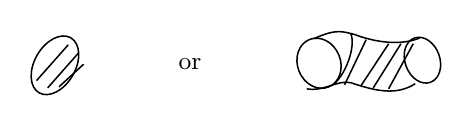
\begin{tikzpicture}[x=.013cm,y=-.013cm,line width=.55pt,font=\small]
\draw[rotate around={-30:(44,86)}] (44,86) ellipse [x radius=20,y radius=31];
\draw (26,101)--(57,66) (37,108)--(67,74) (48,107)--(72,85);
\node at (176,85) {or};
\draw[rotate around={22:(302,84)}] (302,84) ellipse [x radius=21,y radius=25];
\draw[rotate around={20:(403,81)}] (403,81) ellipse [x radius=17,y radius=23];
\draw (297,60)..controls (319,50) and (325,53)..(337,56)
    ..controls (358,64) and (383,67)..(401,59);
\draw (290,109)..controls (307,112) and (320,100)..(333,103)
    ..controls (357,111) and (377,116)..(396,104);
\draw (317,104)..controls (329,93) and (338,67)..(333,55)
 (327,105)--(348,61) (343,106)--(370,65)
 (355,108)--(382,65) (370,109)--(394,65);
\end{tikzpicture}}\endgroup}
\end{GelfandAdjacentEvidence}
\begin{GelfandAdjacentEvidence}{GELFAND-P001056}{6}


\(\delta(\gamma)\) determines the critical phenomena. \(\delta(\gamma)\), apparently depends on the topology.
\Unclear{GELFAND-P001056}{delta-correction}{A short entry after the first \(\delta(\gamma)\) is crossed out. It may be «для» (“for”).}
\end{GelfandAdjacentEvidence}
\begin{GelfandAdjacentEvidence}{GELFAND-P001056}{7}


\SourceFigure{GELFAND-P001056}{bottom-cancel}{\sout{Asymptotics (9).}}
\end{GelfandAdjacentEvidence}



\Needspace{7\baselineskip}
\begin{GelfandAdjacentEvidence}{GELFAND-P001057}{1}
\SourcePage{GELFAND-P001057}{27}
A difficult question: what if we take surfaces with \(\forall\) topology.

How many handles does a typical surface have?

\begin{equation*}
Z_{\beta,\gamma}<\infty\quad\text{when }\beta>\beta_0
\tag{12}
\end{equation*}
\Unclear{GELFAND-P001057}{inequality-12}{The relation sign has been overwritten. Possible readings are \(\beta>\beta_0\) and \(\beta\geqslant\beta_0\).}
\end{GelfandAdjacentEvidence}
\begin{GelfandAdjacentEvidence}{GELFAND-P001057}{2}


\begin{equation*}
Z_{\beta,\gamma}=+\infty\quad\text{when }\beta<\beta_0
  \qquad\text{(like a gas)}
\tag{13}
\end{equation*}
\Unclear{GELFAND-P001057}{inequality-13}{The relation sign has been overwritten. Possible readings are \(\beta<\beta_0\) and \(\beta\leqslant\beta_0\).}
\end{GelfandAdjacentEvidence}
\begin{GelfandAdjacentEvidence}{GELFAND-P001057}{3}


(13): The density of the squares (in \(Z^3\)), belonging to the surface, is positive

(like a Peano curve)
\SourceFigure{GELFAND-P001057}{density-correction}{The abbreviation «пов.» (“surface”) is written over other strokes.}
\end{GelfandAdjacentEvidence}
\begin{GelfandAdjacentEvidence}{GELFAND-P001057}{4}


Conjecture, when \(\beta_0<\beta<\beta_R\) logarithmic fluctuations,

\(\beta>\beta_R\) — \uwave{roughening} (coarsening)

— the shape becomes fixed, almost smooth (almost \(\mathrm{const}\))

Why bother?

\(1^\circ\) NaCl is described by this model

\(2^\circ\) This theory is equivalent to gauge theory \(SU(N)\) in the limit \uwave{\(N\Rightarrow0\)} (!) (degenerate case)
\SourceFigure{GELFAND-P001057}{gauge-limit}{A double arrow follows \(N\).}
\end{GelfandAdjacentEvidence}
\begin{GelfandAdjacentEvidence}{GELFAND-P001057}{5}


\(3^\circ\) It is a fun problem.
\Unclear{GELFAND-P001057}{fun-correction}{A short entry is crossed out after “fun.” It may begin with “pr.”}
\end{GelfandAdjacentEvidence}
\begin{GelfandAdjacentEvidence}{GELFAND-P001057}{6}


\[
w_N(S)\underset{N\to0}{\longrightarrow}w(S)
\]
(Muscovites like to expand in \(1/N\) when \(N\to\infty\)).

\uwave{References.}\quad \dashuline{Phys. Lett.}\quad
\uwave{Amos Maritan, C. Omero}

\underline{Generalizations}\(\rightarrow\)

Continuous case. Surfaces that do not lie on a lattice.

Piecewise linear surfaces made of \(\Delta\)s.

\begin{equation*}
w(S)=e^{-\beta\,\mathrm{area}(S)}
  \frac{\prod e^{-f\,\text{defect }\angle\,\text{at vertices}}}
       {e^{-c\,\#\,\text{handles of }S}}
  \prod_{\text{edges}}\frac{d\ell}{\ell}
\tag{14}
\end{equation*}
\Unclear{GELFAND-P001057}{weight-fraction}{The line above the lower exponential is typeset as a fraction bar. Its placement is visible in the manuscript.}
\end{GelfandAdjacentEvidence}
\begin{GelfandAdjacentEvidence}{GELFAND-P001057}{7}


\SourceFigure{GELFAND-P001057}{regge-reference}{%
\begingroup\color{black}\GelfandFitDiagram{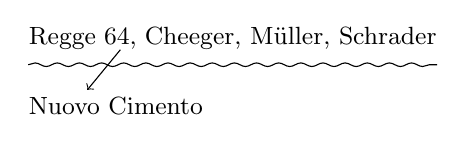
\begin{tikzpicture}[font=\small]
\node[anchor=west,inner sep=0pt] (regge) at (0,0) {Regge};
\node[anchor=west,inner sep=0pt] (year) at ([xshift=2.5pt]regge.east) {64,};
\node[anchor=west,inner sep=0pt] (names) at ([xshift=2.5pt]year.east) {Cheeger, Müller, Schrader};
\node[anchor=west,inner sep=0pt] (journal) at (0,-.85) {Nuovo Cimento};
\draw[->] (year.south)--(.75,-.65);
\draw[decorate,decoration={snake,amplitude=.65pt,segment length=8pt}]
    ([yshift=-.33cm]regge.west)--([yshift=-.33cm]names.east);
\end{tikzpicture}}\endgroup}
\end{GelfandAdjacentEvidence}


\uwave{Question:} convergence when approaching a continuous surface.

\[
R=\sum_f\text{area of }(d-2)\text{ simplex, }f\times\text{defect }\angle
\]
\begin{equation*}
\underline{\text{Theor.}}\quad R\longrightarrow\int\sqrt{g(x)}R(x)d^dx.
\tag{15}
\end{equation*}
\((14)\longrightarrow\) \uwave{Polyakov’s string theory}

\underline{Exercise:} Prove this!


\Needspace{7\baselineskip}
\begin{GelfandAdjacentEvidence}{GELFAND-P001058}{1}
\SourcePage{GELFAND-P001058}{unlabelled}
\uuline{1/\(\overline{\underline{\mathrm{XI}}}\)-82 {}}\qquad\underline{Gelfand Seminar.}

\underline{Zamolodchikov.}

Suppose
\[
[L_n,L_m]=(m-n)L_{n+m}+\frac{c}{12}\delta_{n+m,0}\mathbf1
  \qquad\text{(Virasoro algebra)}
\]
\Unclear{GELFAND-P001058}{virasoro-central}{The central term visibly contains \(\frac{c}{12}\delta_{n+m,0}\mathbf1\).}
\end{GelfandAdjacentEvidence}
\begin{GelfandAdjacentEvidence}{GELFAND-P001058}{2}

and there is a vector \(\lvert0\rangle\), such that
\begin{gather*}
L_n\lvert0\rangle=0,\quad n>0,\\
L_0\lvert0\rangle=\Delta\lvert0\rangle.
\end{gather*}
and
\[
\prod_i(L_{-n_i})^{s_i}\lvert0\rangle=\lvert\psi\rangle
\]
\Unclear{GELFAND-P001058}{vector-correction}{An index after \(L\) is crossed out. It may be \(n_i\) or \(m_i\). The index \(-n_i\) is inserted below.}
\end{GelfandAdjacentEvidence}
\begin{GelfandAdjacentEvidence}{GELFAND-P001058}{3}

(all vectors are obtained in this way)

Suppose \(\varphi(z)\) — an operator acting in this space, and
\[
[L_n,\varphi(z)]=z^{n+1}\frac{d\varphi(z)}{dz}+(n+1)\Delta z^n\varphi(z)
\]
It is uniquely determined by this formula.

\dashuline{First question}: what can be said about it?

— how to calculate
\[
\langle0\lvert\varphi(z_1)\ldots\varphi(z_n)\rvert0\rangle\quad ?
\]
\(L_{-n}^{+}=L_n\), \(\langle0\mid0\rangle=1\Rightarrow\) recover the inner product.

\dashuline{Second question}: what relations on the states can be written down?

Or: is this module irreducible?

\underline{Answer:} (Neretin) degenerate if \(\exists\) natural numbers \(\alpha,\beta\), such that
\Unclear{GELFAND-P001058}{answer-correction}{The crossed-out words before “degenerate” appear to read “irreducible if.”}
\end{GelfandAdjacentEvidence}
\begin{GelfandAdjacentEvidence}{GELFAND-P001058}{4}

\begin{gather*}
\left(-\Delta+\frac{\beta^2-1}{24}(c-13)+\frac{(\alpha\beta-1)}{2}\right)
\left(-\Delta+\frac{(\alpha^2-1)}{24}(c-13)+\frac{(\alpha\beta-1)}{2}\right)\\
{}+\frac{(\alpha^2-\beta^2)^2}{16}=0.
\end{gather*}
\SourceFigure{GELFAND-P001058}{kac-formula-left}{The first factor contains \(\beta^2-1\).}
\end{GelfandAdjacentEvidence}
\begin{GelfandAdjacentEvidence}{GELFAND-P001058}{5}

\SourceFigure{GELFAND-P001058}{kac-formula-right}{The second factor contains \(\alpha^2-1\).}
\end{GelfandAdjacentEvidence}
\begin{GelfandAdjacentEvidence}{GELFAND-P001058}{6}

Degeneracy occurs at \underline{level \(\alpha\beta\)}.

\(\vec{x}(\xi_1,\xi_2)\) — surface, \(g_{ab}(\xi_1,\xi_2)\) — metric, \(a,b=1,2\).
\SourceFigure{GELFAND-P001058}{metric-margin}{\(\mathord{//}\) \(x,g\) are treated as independent variables (the metric is not induced)}
\end{GelfandAdjacentEvidence}
\begin{GelfandAdjacentEvidence}{GELFAND-P001058}{7}


Suppose
\begin{multline*}
Z\equiv\int\mathcal{D}\vec{x}\,\mathcal{D}g_{ab}\,
\exp\left\{-\tfrac12\int\sqrt{g}\,g^{ab}\partial_a\vec{x}\,\partial_b\vec{x}\,d^2\xi\right\}\\
\exp\left\{-\mu_0^2\int\sqrt{g}\,d^2\xi\right\}.
\tag{1}
\end{multline*}
Evaluation — ?

Invariant under the transformations
\[
\begin{cases}
\xi^a\mapsto\xi^a+\varepsilon^a(\xi),\\
g_{ab}(\xi)\mapsto g_{ab}+\nabla_a\varepsilon_b+\nabla_b\varepsilon_a.
\end{cases}
\]
We divide by this group (the volume element is understood to be factored)

— one must integrate over the orbits.

\SourceFigure{GELFAND-P001058}{orbit-sketch}{%
\begingroup\color{black}\GelfandFitDiagram{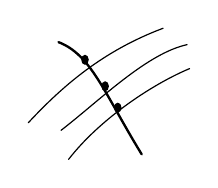
\begin{tikzpicture}[x=.016cm,y=-.016cm,line cap=round]
\draw[line width=.43pt]
  (9,118)..controls(36,89)and(68,61)..(116,43)
  (35,124)..controls(66,100)and(103,63)..(135,56)
  (41,147)..controls(65,116)and(106,88)..(137,75);
\draw[line width=.85pt]
  (33,54)..controls(59,64)and(69,94)..(99,143);
\fill (54,68) ellipse [x radius=3,y radius=4];
\fill (70,89) ellipse [x radius=3,y radius=4];
\fill (80,106) ellipse [x radius=3,y radius=4];
\end{tikzpicture}}\endgroup\par
The strokes thicken at the three intersections. It is unclear whether these are arrowheads.}
\end{GelfandAdjacentEvidence}
\begin{GelfandAdjacentEvidence}{GELFAND-P001058}{8}

Representative: \(\vec{x}(\xi)\) — arbitrary,\quad \(g_{ab}(\xi)=\delta_{ab}\rho(\xi)\)

This gives:
\begin{equation*}
Z=\mathrm{const}\int\mathcal{D}\varphi\,[\det(\Delta_g)]^{-D/2}\,[\det\mathcal{L}]^{1/2},
\tag{2}
\end{equation*}
\Unclear{GELFAND-P001058}{integral-measure}{The symbol after \(\mathcal D\) has a loop on the right. It is provisionally transcribed as \(\varphi\). Another possible reading is \(\psi\).}
\end{GelfandAdjacentEvidence}



\Needspace{7\baselineskip}
\begin{GelfandAdjacentEvidence}{GELFAND-P001059}{1}
\SourcePage{GELFAND-P001059}{38}
where
\Unclear{GELFAND-P001059}{top-cancelled-label}{A short entry in the upper margin is crossed out. Its reading is uncertain.}
\end{GelfandAdjacentEvidence}
\begin{GelfandAdjacentEvidence}{GELFAND-P001059}{2}


\begin{equation*}
(\mathcal L\varepsilon)_a
=\nabla^b\bigl(\nabla_a^a\varepsilon_b+\nabla_b\varepsilon_a
   -g_{ab}\nabla^c\varepsilon_c\bigr).
\tag{3}
\end{equation*}
\Unclear{GELFAND-P001059}{first-derivative}{The first \(\nabla\) in parentheses has a subscript \(a\) and a thickened superscript resembling \(a\). The superscript may be cancelled.}
\end{GelfandAdjacentEvidence}
\begin{GelfandAdjacentEvidence}{GELFAND-P001059}{3}

\Unclear{GELFAND-P001059}{first-term-cancellation}{A vertical entry after the first \(\varepsilon_b\) is crossed out.}
\end{GelfandAdjacentEvidence}
\begin{GelfandAdjacentEvidence}{GELFAND-P001059}{4}


On evaluating this, we obtain:

\SourceFigure{GELFAND-P001059}{field-notation}{The same looped sign appears in (4), (6), and \(\rho=e^\varphi\). It is transcribed as \(\varphi\). Another possible reading is \(\psi\).}
\end{GelfandAdjacentEvidence}
\begin{GelfandAdjacentEvidence}{GELFAND-P001059}{5}


\(D\) — dimension of the space, \(D<26\).
\begin{equation*}
Z=\int\mathcal D\varphi\cdot
  \exp\left\{-\frac{26-D}{48\pi}\int
  \left[\frac12\partial_a\varphi\,\partial_a\varphi+
  m_0^2e^\varphi\right]d^2\xi\right\}.
\tag{4}
\end{equation*}
\(\varphi\) from the formula: \(\rho=e^{\varphi}\).
\[
\Delta_g=\frac{1}{\sqrt g}\partial_a
  \bigl(\sqrt g\,g^{ab}\partial_b\bigr).
\]

The string problem will be solved if we evaluate this integral.

\(D=26\Rightarrow\) the answer is the same as for \(g_{ab}=\delta_{ab}\).

This prescription is used in dual models. They are exact at \(D=26\).

What surfaces should we integrate over?

Surfaces stretched across 2 contours (evolution of a contour).
\Unclear{GELFAND-P001059}{surface-abbreviation}{The abbreviation at the start of the line appears to read «Натян.», for “stretched.”}
\end{GelfandAdjacentEvidence}
\begin{GelfandAdjacentEvidence}{GELFAND-P001059}{6}

\SourceFigure{GELFAND-P001059}{cylinder-contours}{%
\begingroup\color{black}\GelfandFitDiagram{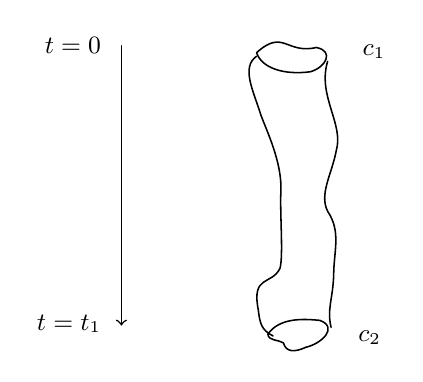
\begin{tikzpicture}[x=.011cm,y=-.011cm,font=\small,line width=.56pt,line cap=round]
\draw[->] (116,40)--(116,363);
\node[anchor=east] at (104,40) {$t=0$};
\node[anchor=east] at (104,361) {$t=t_1$};
\draw (272,48)..controls(303,20)and(306,50)..(341,42)
  ..controls(362,46)and(352,65)..(334,70)
  ..controls(304,74)and(278,66)..(272,48);
\draw (272,52)..controls(254,65)and(268,91)..(277,120)
  ..controls(284,139)and(302,176)..(300,209)
  ..controls(299,237)and(303,282)..(299,297)
  ..controls(289,317)and(266,304)..(274,345)
  ..controls(276,362)and(278,368)..(291,375);
\draw (354,58)..controls(342,98)and(373,130)..(364,161)
  ..controls(359,188)and(344,211)..(354,231)
  ..controls(370,255)and(361,277)..(361,305)
  ..controls(360,333)and(353,344)..(358,365);
\draw (285,373)..controls(298,354)and(325,355)..(345,357)
  ..controls(367,365)and(347,384)..(329,388)
  ..controls(316,394)and(306,394)..(303,383)
  ..controls(297,379)and(286,381)..(285,373);
\node[anchor=west] at (383,47) {$c_1$};
\node[anchor=west] at (378,377) {$c_2$};
\end{tikzpicture}}\endgroup}
\end{GelfandAdjacentEvidence}
\begin{GelfandAdjacentEvidence}{GELFAND-P001059}{7}

\begin{equation*}
Z(c_1,c_2,t_1)\underset{t_1\to\infty}{=}
  \sum_nG(c_1,n)\,G(c_2,n)\,e^{-E_nt_1}.
\tag{5}
\end{equation*}

The spectrum of stationary states in Liouville theory is the QFT spectrum for the Lagrangian
\Unclear{GELFAND-P001059}{liouville-cancellation}{An entry above the words “Liouville theory” is crossed out.}
\end{GelfandAdjacentEvidence}
\begin{GelfandAdjacentEvidence}{GELFAND-P001059}{8}

\begin{equation*}
\int_M\left[\frac12\partial_a\varphi\,\partial_a\varphi+
  m_0^2e^\varphi\right]d^2\xi.
\tag{6}
\end{equation*}

\uwave{Conjecture:} the spectrum is related to the system \(L_n\), described on the previous page.
\begin{gather*}
z=\xi_1+i\xi_2,\\
\bar z=\xi_1-i\xi_2.
\end{gather*}
Traceless two-dimensional conserved energy–momentum tensor:
\[
T_{ab}=\partial_a\varphi\,\partial_b\varphi
   -\tfrac12\delta_{ab}(\partial_c\varphi)^2
   +\alpha\partial_a\partial_b\varphi-\beta\delta_{ab}(\partial_c\varphi)^2.
\]
\SourceFigure{GELFAND-P001059}{tensor-last-term}{The last term reads \(-\beta\delta_{ab}(\partial_c\varphi)^2\).}
\end{GelfandAdjacentEvidence}
\begin{GelfandAdjacentEvidence}{GELFAND-P001059}{9}

\begin{align*}
T&=\varphi_z^2+2\varphi_{zz},&
\partial_{\bar z}T&=0,\\
\bar T&=\varphi_{\bar z}^2+2\varphi_{\bar z\bar z},&
\partial_zT&=0.
\end{align*}
\Unclear{GELFAND-P001059}{tensor-cancelled-index}{The subscript on the first \(T\) is crossed out. It may be \(zz\).}
\end{GelfandAdjacentEvidence}
\begin{GelfandAdjacentEvidence}{GELFAND-P001059}{10}

\SourceFigure{GELFAND-P001059}{lower-holomorphic}{The \(T\) in the second equality on the right has no additional bar.}
\end{GelfandAdjacentEvidence}
\begin{GelfandAdjacentEvidence}{GELFAND-P001059}{11}


\[
\underbrace{T(z)=\sum_{n=-\infty}^{\infty}z^{n-2}L_n}_{\text{(expansion in a series)}}
\qquad\text{— this is where we obtain }L_n!
\]
\SourceFigure{GELFAND-P001059}{series-bracket}{A lower bracket encloses the series and its left-hand side.}
\end{GelfandAdjacentEvidence}



\Needspace{7\baselineskip}
\begin{GelfandAdjacentEvidence}{GELFAND-P001060}{1}
\SourcePage{GELFAND-P001060}{unlabelled}
\uuline{Beilinson A.}

\underline{I.M.G.} Gelfand, Ponomarev (UMN, \(\underset{\text{\scriptsize[2?]}}{\sim}1968\){})
reduced the description of indecomposable representations of the Lorentz group to a problem in linear algebra.
\Unclear{GELFAND-P001060}{reference-leading-mark}{A short mark before “UMN” is crossed out.}
\end{GelfandAdjacentEvidence}
\begin{GelfandAdjacentEvidence}{GELFAND-P001060}{2}

\Unclear{GELFAND-P001060}{reference-lower-mark}{A mark resembling \(2\) appears below \(\sim\).}
\end{GelfandAdjacentEvidence}
\begin{GelfandAdjacentEvidence}{GELFAND-P001060}{3}


\underline{B.}\quad\uwave{model example.} — \(\mathrm{SL}(2,\mathbb R)\)

On \(\mathbb P^1\) we must classify \(D\){}-modules with singularities at two fixed points.

\underline{Theorem 1.} the category of \(D\){}-modules on the disk with a fixed singularity is equivalent to the category
\SourceFigure{GELFAND-P001060}{pointed-disk}{%
\begingroup\color{black}\GelfandFitDiagram{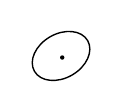
\begin{tikzpicture}[x=1cm,y=1cm,line width=.5pt]
\draw[rotate=30] (0,0) ellipse [x radius=.39,y radius=.28];
\fill (.015,-.02) circle [radius=.028];
\end{tikzpicture}}\endgroup}
\end{GelfandAdjacentEvidence}
\begin{GelfandAdjacentEvidence}{GELFAND-P001060}{4}

\SourceFigure{GELFAND-P001060}{disk-and-pair}{%
\begingroup\color{black}\GelfandFitDiagram{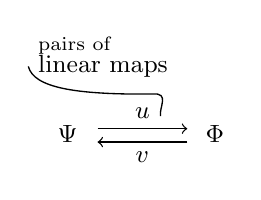
\begin{tikzpicture}[font=\small,line width=.48pt]
\node (linear) at (.65,.64) {linear maps};
\node[anchor=west] at (linear.north west) {\scriptsize pairs of};
\node (psi) at (.2,-.22) {$\Psi$};
\node (phi) at (2.07,-.22) {$\Phi$};
\draw[->] (.58,-.15)--node[above]{$u$}(1.72,-.15);
\draw[->] (1.72,-.32)--node[below]{$v$}(.58,-.32);
\draw (linear.west)..controls(-.23,.37)and(.3,.28)..(1.28,.29)
  ..controls(1.5,.31)and(1.36,.12)..(1.38,.01);
\end{tikzpicture}}\endgroup\par
“Pairs of” is written above “linear maps.”}
\end{GelfandAdjacentEvidence}
\begin{GelfandAdjacentEvidence}{GELFAND-P001060}{5}

such that \(uv-\mathrm{Id}\) \uwave{is invertible}.
\SourceFigure{GELFAND-P001060}{bracketed-description}{%
\(\left[\left(\begin{array}{l}
 \text{outside }0\text{ — smooth }=\\
 =\text{bundles with connection};\\
 \text{at }0\text{ — regular singularity.}
\end{array}\right)\right]\)}
\end{GelfandAdjacentEvidence}
\begin{GelfandAdjacentEvidence}{GELFAND-P001060}{6}


\underline{Geometric problem.}
\SourceFigure{GELFAND-P001060}{geometric-inclusions}{%
\begingroup\color{black}\GelfandFitDiagram{\begin{tikzcd}[ampersand replacement=\&,column sep=small]
Y \arrow[r,hook,"i"] \& X \& U=X\setminus Y \arrow[l,hook',"j"']
\end{tikzcd}}\endgroup}
\end{GelfandAdjacentEvidence}
\begin{GelfandAdjacentEvidence}{GELFAND-P001060}{7}

A sheaf on \(X\) is given as follows:
\[
\mathcal F_X=(\mathcal F_U,\mathcal F_Y,\quad
  \mathcal F_Y\longrightarrow i^*j_*\mathcal F_U)
\]
(gluing function)
\Unclear{GELFAND-P001060}{gluing-cancellation}{A short entry between “function” and “gluing” is crossed out. It may begin with «ск».}
\end{GelfandAdjacentEvidence}
\begin{GelfandAdjacentEvidence}{GELFAND-P001060}{8}


For representations we must solve the analogous problem on the space of flags.

\Unclear{GELFAND-P001060}{cancelled-equation}{The crossed-out formula may read \(Y=f^{-1}(0)\).}
\end{GelfandAdjacentEvidence}
\begin{GelfandAdjacentEvidence}{GELFAND-P001060}{9}


\underline{Theorem.} the category of \(D\){}-modules with regular singularities on \(X\) is equivalent to the category of tuples
\SourceFigure{GELFAND-P001060}{module-pair}{%
\begingroup\color{black}\GelfandFitDiagram{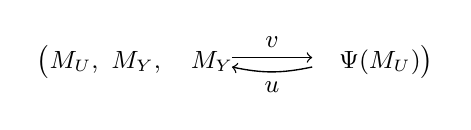
\begin{tikzpicture}[font=\small,line width=.49pt]
\node at (0,0) {$\bigl(M_U,\ M_Y,\quad M_Y$};
\node at (3.19,0) {$\Psi(M_U)\bigr)$};
\draw[->] (1.23,.055)--node[above]{$v$}(2.25,.055);
\draw[->] (2.25,-.065) to[bend left=12] node[below]{$u$}(1.23,-.065);
\end{tikzpicture}}\endgroup}
\end{GelfandAdjacentEvidence}
\begin{GelfandAdjacentEvidence}{GELFAND-P001060}{10}

\(vu=N\) — something.
\Unclear{GELFAND-P001060}{bottom-cancellation}{A short entry after “something” is crossed out.}
\end{GelfandAdjacentEvidence}



\Needspace{7\baselineskip}
\begin{GelfandAdjacentEvidence}{GELFAND-P001061}{1}
\SourcePage{GELFAND-P001061}{48}
\uuline{15/\(\overline{\underline{\mathrm{XI}}}\)-82 {}}\qquad\underline{Gelfand Seminar.}

\uuline{I.M.G.}\quad\underline{Problem}. (imprecise)

\(G_{n,k}\) — Grassmannian, \(k\){}-dimensional planes in an \(n\){}-dimensional space.
\Unclear{GELFAND-P001061}{top-cancelled-symbol}{An entry at the start of the line is crossed out. It resembles \(G\) with additional marks.}
\end{GelfandAdjacentEvidence}
\begin{GelfandAdjacentEvidence}{GELFAND-P001061}{2}


Cohomology is calculated using Schubert cells.
\Unclear{GELFAND-P001061}{schubert-initial-phrase}{The first two abbreviations provisionally read «Когом. счит.», for “cohomology is calculated.”}
\end{GelfandAdjacentEvidence}
\begin{GelfandAdjacentEvidence}{GELFAND-P001061}{3}


(The \dashuline{cell} is specified by the dimensions of intersections with the flag
\begin{gather*}
0=d_0\leqslant d_1\leqslant d_2\leqslant\ldots\leqslant d_n=k,\\
\dim\text{ of the cell}=\sum d_j.
\end{gather*}
)
\SourceFigure{GELFAND-P001061}{schubert-dimension}{The dimension formula reads \(\sum d_j\).}
\end{GelfandAdjacentEvidence}
\begin{GelfandAdjacentEvidence}{GELFAND-P001061}{4}


Consider a \(\mathrm{II}_1\){} factor. In it, consider \(\alpha\){}-dimensional projections (a continuous analogue of Grassmannians).
\uwave{Is there an analogue of a Schubert cell?}

\uwave{Flag of continuous dimension \([0,1]\).}

Does this give a Grassmannian?

Continuous cohomology!?

\uwave{Conjecture}: described by monotone functions.
\Unclear{GELFAND-P001061}{hypothesis-cancellation}{A short entry after “Conjecture” is crossed out.}
\end{GelfandAdjacentEvidence}
\begin{GelfandAdjacentEvidence}{GELFAND-P001061}{5}


An even vaguer question: what topology? and what cohomology?
\Unclear{GELFAND-P001061}{question-leading-cancellation}{A mark before “An even” is crossed out.}
\end{GelfandAdjacentEvidence}
\begin{GelfandAdjacentEvidence}{GELFAND-P001061}{6}


\uuline{Yu. I. Manin.}

1) Flag supermanifolds

2) The Radon–Penrose transform in a supermathematical setting.
\Unclear{GELFAND-P001061}{agenda-cancelled-letter}{A single mark is crossed out before “supermathematical.”}
\end{GelfandAdjacentEvidence}
\begin{GelfandAdjacentEvidence}{GELFAND-P001061}{7}


3) Applications to solving nonlinear equations: new solutions of the non-self-dual Yang–Mills equations

(ordinary and supersymmetric)

4) Specific flag manifolds, their deformation, and so on in supersymmetry and supergravity.

5) The problem of the index and of characteristic classes.
\SourceFigure{GELFAND-P001061}{agenda-annotations}{[Below “of the index”] (has not really been done)\par [Below “of characteristic classes”] (A. S. Schwarz did something important)}
\end{GelfandAdjacentEvidence}
\begin{GelfandAdjacentEvidence}{GELFAND-P001061}{8}


The talk will cover 1)–4)

\medskip
1) \underline{Reminder about the self-dual Yang–Mills equations}

\(T=\mathbb C^4\)\qquad [antiholomorphic involution \(T\oplus T^*\)]
\SourceFigure{GELFAND-P001061}{involution-abbreviation}{The first abbreviation appears to read «антиголом.», for “antiholomorphic.”}
\end{GelfandAdjacentEvidence}
\begin{GelfandAdjacentEvidence}{GELFAND-P001061}{9}

\SourceFigure{GELFAND-P001061}{involution-relation}{The sign between \(T\) and \(T^*\) is \(\oplus\).}
\end{GelfandAdjacentEvidence}
\begin{GelfandAdjacentEvidence}{GELFAND-P001061}{10}


\(\dim G(2,T)=4\) = complex compact Minkowski space.

3-dimensional cell (family, parametrized by a group [one uncertain abbreviation])
\Unclear{GELFAND-P001061}{three-cell-description}{The abbreviation before “group” may read «разн.» or «разл.».}
\end{GelfandAdjacentEvidence}
\begin{GelfandAdjacentEvidence}{GELFAND-P001061}{11}


\SourceFigure{GELFAND-P001061}{cone-sketch}{%
\begingroup\color{black}\GelfandFitDiagram{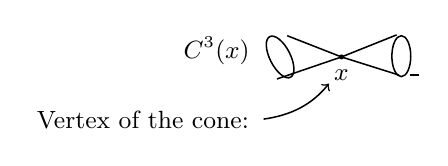
\begin{tikzpicture}[x=.010cm,y=-.010cm,font=\small,line width=.55pt]
\node[anchor=east] at (-104,-8) {$C^3(x)$};
\draw (-69,-27)--(0,0)--(-82,28);
\draw[rotate around={27:(-78,0)}] (-78,0) ellipse [x radius=13,y radius=29];
\draw (0,0)--(70,-28) (0,0)--(73,23);
\draw (76,-1) ellipse [x radius=12,y radius=26];
\draw (87,23)--(98,23);
\fill (0,0) circle [radius=3.2];
\node[below] at (0,3) {$x$};
\draw[->] (-99,79)..controls(-64,74)and(-38,61)..(-16,34);
\node[anchor=east] at (-105,80) {Vertex of the cone:};
\end{tikzpicture}}\endgroup\par
(determined by a point).}
\end{GelfandAdjacentEvidence}
\begin{GelfandAdjacentEvidence}{GELFAND-P001061}{12}


\[
M^4=\text{real part of }G(2,T)\setminus C^3(\infty)
\ \leftarrow\ \infty\text{-cone}.
\]

2-dimensional cells: 2 types

\[
C^2_{\underset{+}{\alpha},\underset{-}{\beta}}
  (x,\mathbb C^2\subset T_xM)
  \text{ — }\pm\text{-planes},\quad(\alpha,\beta)\text{-planes}.
\]
\SourceFigure{GELFAND-P001061}{plane-symbol}{Inside the parentheses, the symbol before \(\subset\) is a double-stroked \(\mathbb C\) with superscript \(2\).}
\end{GelfandAdjacentEvidence}
\begin{GelfandAdjacentEvidence}{GELFAND-P001061}{13}

\SourceFigure{GELFAND-P001061}{plane-signs}{The \(+\) is written below \(\alpha\), and the \(-\) below \(\beta\).}
\end{GelfandAdjacentEvidence}



\Needspace{7\baselineskip}
\begin{GelfandAdjacentEvidence}{GELFAND-P001062}{1}
\SourcePage{GELFAND-P001062}{unlabelled}
\(C^1\) — null lines (light rays)

\SourceFigure{GELFAND-P001062}{tautological-bundles}{%
\begingroup\color{black}\GelfandFitDiagram{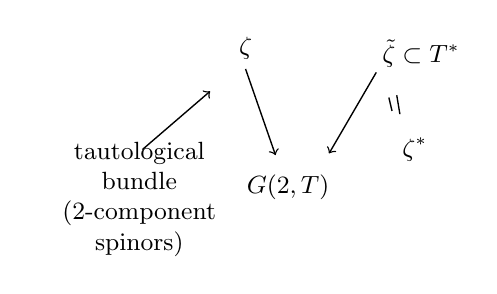
\begin{tikzpicture}[font=\small,line width=.5pt]
\node (base) at (1.4,-.8) {$G(2,T)$};
\node (left) at (.86,.97) {$\zeta$};
\node (right) at (3.09,.9) {$\tilde{\zeta}\subset T^*$};
\node (dual) at (3.01,-.32) {$\zeta^*$};
\draw[->] (left.south)--(1.24,-.39);
\draw[->] (2.52,.66)--(1.92,-.37);
\draw (2.68,.34)--(2.72,.17) (2.78,.37)--(2.82,.13);
\node[align=center,text width=2.6cm] at (-.49,-.95) {tautological bundle\\(2-component spinors)};
\draw[->] (-.45,-.32)--(.41,.42);
\end{tikzpicture}}\endgroup\par
The bundle symbol is provisionally transcribed as \(\zeta\). The meaning of the two strokes below the right-hand label is uncertain.}
\end{GelfandAdjacentEvidence}
\begin{GelfandAdjacentEvidence}{GELFAND-P001062}{2}


\underline{Problem.}\qquad \(G(2,T)\)

Describe the superhomogeneous complex manifolds \(M\), for which \(M_{\mathrm{red}}=G(2,T)\).

Condition: \(M\) — a flag manifold for simple Lie supergroups of classical type.

\underline{List (beginning)}.

\[
\text{a)}\quad F(2|0,2|N,\mathbb C^{4|N})=M
\]
\Unclear{GELFAND-P001062}{cancelled-flag-argument}{A mark resembling \(2\) is crossed out after \(2\mid N\).}
\end{GelfandAdjacentEvidence}
\begin{GelfandAdjacentEvidence}{GELFAND-P001062}{3}

(flags of dimensions \(2|0,2|N\) in \(\mathbb C^{4|N}\)).
\[
N=0,1,2,3,\ldots
\qquad
\mathbb C^{4|N}=(\mathbb C^4)_0\oplus(\mathbb C^N)_1.
\]
\SourceFigure{GELFAND-P001062}{superdimension-arrow}{%
\begingroup\color{black}\GelfandFitDiagram{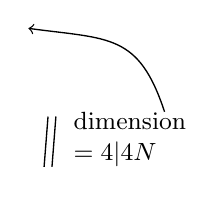
\begin{tikzpicture}[font=\small,line width=.48pt]
\draw[->] (1.48,.3)..controls(1.15,1.3)and(.78,1.22)..(-.25,1.36);
\draw (0,.24)--(-.05,-.4) (.1,.24)--(.05,-.4);
\node[align=left,anchor=west] at (.2,-.05) {dimension\\$=4|4N$};
\end{tikzpicture}}\endgroup\par
The note “dimension \(=4\mid4N\)” is to the right of the inclusions. The arrow points up and to the left.}
\end{GelfandAdjacentEvidence}
\begin{GelfandAdjacentEvidence}{GELFAND-P001062}{4}


Naïve definition:
\[
\text{points }x\in F(2|0,2|N,\mathbb C^{4|N})
  =\underline{\mathbb C^{2|0}\subset\mathbb C^{2|N}}\subset\mathbb C^{4|N}.
\]
But there are too few coordinates.

\uwave{Correct definition}: \(\forall\) supercommutative \(\mathbb C\)-algebra \(A\) we specify \(M(A)\)
and now we also specify \([A\overset f\longrightarrow B]\)
\[
\begin{array}{r@{\quad}l}
M(A):={}&N^{2|0}\subset N^{2|N}\subset A\otimes_{\mathbb C}\mathbb C^{4|N}\\
\downarrow&\text{(projective)}\\
M(B)&\text{direct submodules}
\end{array}
\]
\SourceFigure{GELFAND-P001062}{functor-diagram}{The arrow goes from \(M(A)\) to \(M(B)\). The submodule description is written below the inclusions.}
\end{GelfandAdjacentEvidence}
\begin{GelfandAdjacentEvidence}{GELFAND-P001062}{5}


\dashuline{Coordinates:}\quad
\(G(1|0,\mathbb C^{m|n}):=P^{m-1|n}\supset P\).
\SourceFigure{GELFAND-P001062}{projective-point-symbol}{The symbol to the right of \(\supset\) appears to be \(P\).}
\end{GelfandAdjacentEvidence}
\begin{GelfandAdjacentEvidence}{GELFAND-P001062}{6}


Homogeneous coordinates: \((x_1,\ldots,x_m;\xi_1,\ldots,\xi_n)\).
\[
\text{Cover } P^{m-1,n}=\bigcup_{i=1}^{m}U_i,\quad
U_i:\left(\frac{x_1}{x_i},\ldots,\frac{x_m}{x_i},
          \frac{\xi_1}{x_i},\ldots,\frac{\xi_m}{x_i}\right).
\]
\SourceFigure{GELFAND-P001062}{affine-first-odd}{The denominator of the first odd coordinate appears to be \(x_i\).}
\end{GelfandAdjacentEvidence}
\begin{GelfandAdjacentEvidence}{GELFAND-P001062}{7}

\SourceFigure{GELFAND-P001062}{affine-last-index}{The final fraction reads \(\xi_m/x_i\). The list of homogeneous coordinates ends in \(\xi_n\).}
\end{GelfandAdjacentEvidence}
\begin{GelfandAdjacentEvidence}{GELFAND-P001062}{8}


\uwave{Exercise}: relate this to the preceding discussion (big cells).

\uwave{We can have:} \(\xi_i=0\) — a cell of codimension \(0|1\).

It is unclear in which cohomology they lie?

Differential and integral forms are also insufficient. (they serve the extreme dimensions)
\Unclear{GELFAND-P001062}{forms-abbreviation}{The abbreviation appears to be «обслуж.», for “serve.”}
\end{GelfandAdjacentEvidence}
\begin{GelfandAdjacentEvidence}{GELFAND-P001062}{9}


Schwarz’s objects are intermediate but have strange properties.

Real points of the big cell in \(F(2|0,2|N;\mathbb C^{4|N})=\)
\[
=N\text{-extended }\underline{\text{physicists’ superspace}}:
 (x^m;\theta_{\alpha i},\theta^{\beta i}).
\]
\dashuline{Requirement}: [inserted existence of] \sout{conformal}
conformal completion.
\SourceFigure{GELFAND-P001062}{completion-insertion}{“Existence” is written with an insertion mark. The earlier “conformal” is crossed out.}
\end{GelfandAdjacentEvidence}
\begin{GelfandAdjacentEvidence}{GELFAND-P001062}{10}


\[
\text{b)}\quad FI(2|0,2|2,\mathbb C^{4|4},\Pi\mathrm{Sp})
  \qquad \text{dimension}=4|8.
\]
\Unclear{GELFAND-P001062}{cancelled-isotropic-argument}{An entry before \(\mathbb C^{4\mid4}\) is crossed out. It may read \(\mathrm{OSp}\).}
\end{GelfandAdjacentEvidence}



\Needspace{7\baselineskip}
\begin{GelfandAdjacentEvidence}{GELFAND-P001063}{1}
\SourcePage{GELFAND-P001063}{49}
\(I\) — isotropic,\quad \(\Pi\mathrm{Sp}\) — the type of form with respect to which the flags are isotropic.

(odd symmetric form)

There are also \underline{series} and \underline{isolated} manifolds.
\Unclear{GELFAND-P001063}{cancelled-word}{A word before “There are also” is crossed out. It may read «Бывают» (“there are”) or «Будут» (“there will be”).}
\end{GelfandAdjacentEvidence}


\[
2)\quad M=G(2,T),\qquad \underline{P(T)}=\underline{G(1,T)}.
\]


\Needspace{7\baselineskip}
\begin{GelfandAdjacentEvidence}{GELFAND-P001064}{1}
\SourcePage{GELFAND-P001064}{unlabelled}
\underline{22/\(\overline{\underline{\mathrm{XI}}}\)-82 {}}\qquad
\uuline{Gelfand Seminar.}

\uuline{A. M. Polyakov.}

(Alexander Markovich).

The string problem
\SourceFigure{GELFAND-P001064}{string-caption}{%
\begingroup\color{black}\GelfandFitDiagram{\begin{tikzpicture}[x=.031cm,y=-.031cm,line width=.55pt]
\draw (51,13)..controls(75,18)and(102,23)..(115,41)
 ..controls(139,80)and(104,108)..(81,111)
 ..controls(47,110)and(30,95)..(30,77)
 ..controls(28,63)and(7,21)..(41,13);
\end{tikzpicture}}\endgroup\par
— elem. excitation.}
\end{GelfandAdjacentEvidence}
\begin{GelfandAdjacentEvidence}{GELFAND-P001064}{2}


Reduces to the following: there is a field
\[
\varphi=\varphi(\xi_1,\xi_2)\qquad
  (\sim\text{ surface in isothermal coordinates})
\]
\begin{equation*}
g_{ab}(\xi)=e^{\varphi(\xi)}\delta_{ab}.
\tag{1}
\end{equation*}
\begin{equation*}
\mathcal L=\frac1\gamma\left\{\frac12(\partial_a\varphi)^2+e^\varphi\right\},
\qquad S=\int\mathcal L\,d^2\xi,
\tag{2}
\end{equation*}
\begin{equation*}
\frac1\gamma=\frac{26-D}{48\pi}
\tag{3}
\end{equation*}
(\(D\) — dimension of the space into which the two-dimensional surface under consideration is embedded)

Why does it have the form (2) (apart from \(\gamma\))?

Fix the metric (1). The remaining freedom: conformal transformations.
\begin{equation*}
e^{\widetilde\varphi(z,\bar z)}
=\left|\frac{dw}{dz}\right|^2 e^{\varphi(w(z),\overline w(z))}.
\tag{4}
\end{equation*}
\SourceFigure{GELFAND-P001064}{conformal-last-argument}{In the exponent on the right, the second \(w\) has a bar. The final \(z\) has none.}
\end{GelfandAdjacentEvidence}
\begin{GelfandAdjacentEvidence}{GELFAND-P001064}{3}

\SourceFigure{GELFAND-P001064}{transformation-margin}{At the right of the formula is “(2)” with an additional stroke.}
\end{GelfandAdjacentEvidence}
\begin{GelfandAdjacentEvidence}{GELFAND-P001064}{4}


Lagrangian (2) — the only local Lagrangian (depending only on the value of the function and its derivatives at the point), invariant under transformation (4).

\(\mathcal L\) is called \uwave{the Liouville Lagrangian}
(the corresponding equation \(\Delta\varphi=e^\varphi\) or \(\partial^2\varphi=e^\varphi\)).
\Unclear{GELFAND-P001064}{liouville-cancelled-symbol}{A bracket-like mark after the first \(e^\varphi\) is crossed out.}
\end{GelfandAdjacentEvidence}



\Needspace{7\baselineskip}
\begin{GelfandAdjacentEvidence}{GELFAND-P001065}{1}
\SourcePage{GELFAND-P001065}{unlabelled}
\begin{equation*}
\partial^2\varphi\equiv\Delta\varphi=e^\varphi.\tag{5}
\end{equation*}
\uwave{Can be solved explicitly.}\quad (\(\sim\) curvature is constant)

Classical solution of equation (5):
\begin{equation*}
\varphi=\log\left(\frac{|\partial_z w|^2}{(\operatorname{Im}w)^2}\right),
\qquad w(z)\text{ — any holomorphic function}.
\tag{6}
\end{equation*}

Consider a sphere with punctures that are at \(\infty\) in the sense of the metric.
\SourceFigure{GELFAND-P001065}{punctured-sphere}{%
\begingroup\color{black}\GelfandFitDiagram{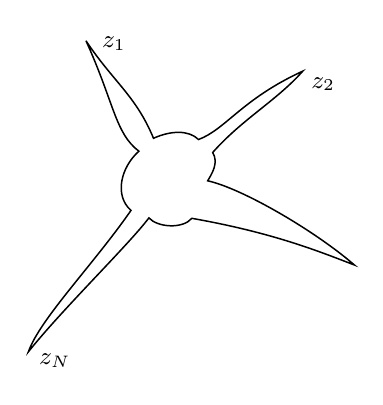
\begin{tikzpicture}[x=.0053cm,y=-.0053cm,font=\small,line width=.54pt]
\draw (154,32)..controls(219,130)and(274,164)..(316,266)
 ..controls(358,247)and(401,246)..(424,269)
 ..controls(490,244)and(528,172)..(674,105)
 ..controls(611,176)and(530,219)..(458,300)
 ..controls(473,325)and(456,351)..(446,368)
 ..controls(528,386)and(702,487)..(798,570)
 ..controls(717,539)and(606,493)..(408,458)
 ..controls(386,484)and(326,480)..(305,457)
 ..controls(255,523)and(101,672)..(16,778)
 ..controls(44,699)and(171,570)..(262,439)
 ..controls(221,403)and(238,335)..(281,297)
 ..controls(224,254)and(222,182)..(154,32);
\node[anchor=west] at (169,39) {$z_1$};
\node[anchor=west] at (671,136) {$z_2$};
\node[anchor=west] at (18,799) {$z_N$};
\end{tikzpicture}}\endgroup}
\end{GelfandAdjacentEvidence}
\begin{GelfandAdjacentEvidence}{GELFAND-P001065}{2}

\[
e^\varphi\underset{z\to z_i}{\longrightarrow}
  \frac{2}{|z-z_i|^2\log^2|z-z_i|}.
\]
we want to calculate the quantum quantity
\begin{equation*}
\Psi(z_1,\ldots,z_N)=\int\mathcal D\varphi(z)e^{-S(\varphi)}
\underset{\gamma\to0}{\simeq}e^{-S_{\mathrm{cl}}(z_1,\ldots,z_N)}.
\tag{7}
\end{equation*}
Let us calculate \(S_{\mathrm{cl}}\).

(8)
\SourceFigure{GELFAND-P001065}{covering-diagram}{%
\begingroup\color{black}\GelfandFitDiagram{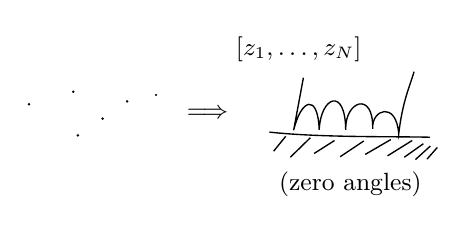
\begin{tikzpicture}[x=.0059cm,y=-.0059cm,font=\small,line width=.49pt]
\fill (36,175) circle [radius=3] (131,148) circle [radius=3]
 (194,206) circle [radius=3] (247,169) circle [radius=3]
 (309,155) circle [radius=2.5] (141,242) circle [radius=3];
\node at (420,196) {$\Longrightarrow$};
\node at (616,57) {$[z_1,\ldots,z_N]$};
\draw (553,235)..controls(664,247)and(817,244)..(898,246);
\draw (626,118)--(605,231)
 ..controls(621,164)and(657,150)..(660,230)
 ..controls(663,159)and(716,136)..(717,230)
 ..controls(715,168)and(777,145)..(775,228)
 ..controls(772,186)and(826,167)..(831,239)
 ..controls(839,169)and(855,136)..(864,105);
\draw (588,244)--(562,276) (641,247)--(598,289)
 (693,253)--(649,281) (756,254)--(705,288)
 (814,251)--(759,283) (860,253)--(807,286)
 (884,260)--(843,289) (899,265)--(867,294)
 (914,268)--(892,293);
\node[anchor=north] at (727,300) {(zero angles)};
\end{tikzpicture}}\endgroup\par
The caption below the drawing appears to read “zero angles.”}
\end{GelfandAdjacentEvidence}
\begin{GelfandAdjacentEvidence}{GELFAND-P001065}{3}

\SourceFigure{GELFAND-P001065}{covering-caption}{(covering surface)}
\end{GelfandAdjacentEvidence}
\begin{GelfandAdjacentEvidence}{GELFAND-P001065}{4}


Let us calculate the energy–momentum tensor:
\begin{equation*}
\begin{gathered}
T=\tfrac12(\partial_z\varphi)^2-\partial_z^2\varphi,\\
T=T_{11}-T_{22}+2iT_{12},\qquad T_{11}+T_{22}=0.
\end{gathered}
\tag{9}
\end{equation*}
(\(T_{ij}\) is recovered from \(T\), since \(T_{ij}\) — real)

\begin{equation*}
T(z|z_1,\ldots,z_N)
=\underset{\text{(Schwarzian derivative)}}{\mathcal D}[w(z)]
=\frac{w'''}{w'^2}-\frac32\frac{(w'')^2}{(w')^4}.
\tag{10}
\end{equation*}
\SourceFigure{GELFAND-P001065}{schwarzian-denominators}{The denominators read \(w'^2\) and \((w')^4\).}
\end{GelfandAdjacentEvidence}
\begin{GelfandAdjacentEvidence}{GELFAND-P001065}{5}

(invariant under fractional linear transformations)
\[
\widetilde w(z)=\frac{\alpha w+\beta}{\gamma w+\delta}.
\]
Hence \(T\) — is single-valued and has only poles:
\begin{equation*}
T(z|z_1,\ldots,z_N)=\frac14\sum_1^N\frac1{(z-z_i)^2}
 +\sum_1^N\frac{c_i(z_1,\ldots,z_N)}{z-z_i}.
\tag{11}
\end{equation*}
\Unclear{GELFAND-P001065}{cancelled-pole-denominator}{An entry before \(z-z_i\) in the final denominator is heavily crossed out.}
\end{GelfandAdjacentEvidence}
\begin{GelfandAdjacentEvidence}{GELFAND-P001065}{6}


It is important that \(c_i\) be real, and this determines \(c_i\) {}.

(\(c_i\) — accessory coefficients)
\SourceFigure{GELFAND-P001065}{monodromy-insertion}{In small handwriting above (12), “This is connected with the real monodromy coefficients of the equation.”}
\end{GelfandAdjacentEvidence}
\begin{GelfandAdjacentEvidence}{GELFAND-P001065}{7}


\Unclear{GELFAND-P001065}{cancelled-before-ode}{A phrase before (12) is crossed out. It may read “this is connected.”}
\end{GelfandAdjacentEvidence}
\begin{GelfandAdjacentEvidence}{GELFAND-P001065}{8}

\begin{equation*}
\psi''+T(z)\psi=0.\tag{12}
\end{equation*}
\begin{equation*}
w(z)=\frac{\psi_1(z)}{\psi_2(z)}.\tag{13}
\end{equation*}
(\(\psi_1,\psi_2\) — 2 linearly independent solutions of (13))
\SourceFigure{GELFAND-P001065}{solution-equation-reference}{The reference after “solutions” is “(13).”}
\end{GelfandAdjacentEvidence}


\uwave{Condition on variation of \(c\)}: the monodromy changes but remains real,

(this is the problem)

(in \(\mathrm{SL}(2,\mathbb R)\), as opposed to \(\mathrm{SL}(2,\mathbb C)\))


\Needspace{7\baselineskip}
\begin{GelfandAdjacentEvidence}{GELFAND-P001066}{1}
\SourcePage{GELFAND-P001066}{55}
Relation:
\begin{equation*}
c_i(z_1,\ldots,z_N)=\frac{\partial S_{\mathrm{cl}}}{\partial z_i}.
\tag{14}
\end{equation*}
\SourceFigure{GELFAND-P001066}{ornament-under-fourteen}{%
\(\rule{1.45em}{.35pt}\,\boldsymbol{\cdot}\,\rule{1.7em}{.35pt}\)}
\end{GelfandAdjacentEvidence}
\begin{GelfandAdjacentEvidence}{GELFAND-P001066}{2}


The problem is solved via the quantum problem, then the semiclassical limit as \(\gamma\to0\)!
\SourceFigure{GELFAND-P001066}{quasiclassical-parameter}{The parameter in the semiclassical limit is transcribed as \(\gamma\).}
\end{GelfandAdjacentEvidence}
\begin{GelfandAdjacentEvidence}{GELFAND-P001066}{3}

\begin{equation*}
[T(z_1),T(z_2)]
  =\bigl(T(z_1)+T(z_2)\bigr)\delta'(z_1-z_2)
   +\frac{c}{12}\delta'''(z_1-z_2).
\tag{15}
\end{equation*}
\Unclear{GELFAND-P001066}{eq15-superscript-correction}{A small superscript over \(z_2\) on the left of the first (15) is crossed out. It may be a digit.}
\end{GelfandAdjacentEvidence}
\begin{GelfandAdjacentEvidence}{GELFAND-P001066}{4}


(the dependence on \(z_1,\ldots,z_N\) is left unwritten)
\Unclear{GELFAND-P001066}{eq15-crossed-mark}{A mark before the parenthesis is heavily crossed out.}
\end{GelfandAdjacentEvidence}
\begin{GelfandAdjacentEvidence}{GELFAND-P001066}{5}


or:
\begin{equation*}
[T(z),T(w)]
  =\bigl(T(z)+T(w)\bigr)\delta'(z-w)
   +\frac{c}{12}\delta'''(z-w)
\tag{15}
\end{equation*}
(in the classical case. Poisson brackets)

Let us calculate:

Lagrangian:
\[
\mathcal L=\int\bigl(\partial_z\varphi\,\partial_{\bar z}\varphi-e^\varphi\bigr)
\]
\begin{equation*}
p=\frac{\partial\mathcal L}{\partial(\partial_{\bar z}\varphi)}
  =\partial_{\bar z}\varphi
\tag{16}
\end{equation*}
\SourceFigure{GELFAND-P001066}{eq16-right-index}{On the right of (16), a separate bar is visible over the subscript \(z\).}
\end{GelfandAdjacentEvidence}
\begin{GelfandAdjacentEvidence}{GELFAND-P001066}{6}

\SourceFigure{GELFAND-P001066}{virasoro-margin}{[In the right margin] Virasoro}
\end{GelfandAdjacentEvidence}
\begin{GelfandAdjacentEvidence}{GELFAND-P001066}{7}


whence
\begin{equation*}
\{\varphi(z),\partial_w\varphi(w)\}=\gamma\delta(z-w).
\tag{17}
\end{equation*}
\Unclear{GELFAND-P001066}{eq17-before-delta}{A separate mark before \(\delta\) appears to be \(\gamma\).}
\end{GelfandAdjacentEvidence}
\begin{GelfandAdjacentEvidence}{GELFAND-P001066}{8}

\(\{T(z),T(w)\}\) and so on.

Expand in a Laurent series:
\begin{equation*}
T(z)=\sum_n(L_n z^n+L_{-n}z^{-n})
\tag{18}
\end{equation*}
\begin{equation*}
[L_n,L_m]=(n-m)L_{n+m}+\frac{c}{12}n(n^2-1),
\quad c=26-D.
\tag{19}
\end{equation*}
\SourceFigure{GELFAND-P001066}{eq19-central-term}{A comma follows \(n(n^2-1)\) in (19).}
\end{GelfandAdjacentEvidence}
\begin{GelfandAdjacentEvidence}{GELFAND-P001066}{9}

(this could have been predicted from the Gelfand–Fuchs result, from the form of the central extension)

\[
\widetilde z=z+\varepsilon(z)\qquad\text{(variation)}
\]
\[
\delta\varphi=\operatorname{Re}
  \bigl(\varepsilon(z)\partial_z\varphi+\partial_z\varepsilon\bigr)
\]
A number is added to the action \(\rightsquigarrow\) a central extension appears).
\SourceFigure{GELFAND-P001066}{central-extension-arrow}{A wavy arrow connects the two phrases.}
\end{GelfandAdjacentEvidence}
\begin{GelfandAdjacentEvidence}{GELFAND-P001066}{10}


Let us try to find \(\Psi\) purely algebraically:
\begin{equation*}
\text{Let}\qquad T_\varepsilon=\int\varepsilon(z)T(z)\,d^2z
\tag{20}
\end{equation*}
\SourceFigure{GELFAND-P001066}{shift-generator}{%
\(\longleftarrow\) Suppose it is the generator of the shift.}
\end{GelfandAdjacentEvidence}
\begin{GelfandAdjacentEvidence}{GELFAND-P001066}{11}

\begin{equation*}
\delta_\varepsilon\psi=[T_\varepsilon,\psi(z)]
 =\varepsilon(z)\frac{d\psi}{dz}+\Delta\cdot\varepsilon'(z)\psi(z)
\tag{21}
\end{equation*}
(variation of the field \(\psi\))
\begin{equation*}
[L_n,\psi(z)]
 =z^{n+1}\frac{d\psi}{dz}+(n+1)\Delta\psi(z).
\tag{22}
\end{equation*}
\SourceFigure{GELFAND-P001066}{eq22-weight-term}{The second term of (22) reads \((n+1)\Delta\psi(z)\).}
\end{GelfandAdjacentEvidence}


\(\psi(z)\) — an operator in the same space on which the representation is defined.


\Needspace{7\baselineskip}
\begin{GelfandAdjacentEvidence}{GELFAND-P001067}{1}
\SourcePage{GELFAND-P001067}{unlabelled}
$\psi(z)$ is the operator creating a horn on the sphere.
\begin{equation*}
\Psi(z)|v\rangle.
\end{equation*}
\SourceFigure{GELFAND-P001067}{initial-ket-glyph}{Uppercase $\Psi$ in the ket line.}
\end{GelfandAdjacentEvidence}
\begin{GelfandAdjacentEvidence}{GELFAND-P001067}{2}

Consider the functions:
\begin{equation*}
\langle v|\psi(z_1)\psi(z_2)\psi(z_3)\psi(z_4)|v\rangle
\tag{23}
\end{equation*}
\begin{equation*}
\Psi(x)=\langle v|\psi(\infty)\psi(1)\psi(x)\psi(0)|v\rangle
\end{equation*}
\begin{equation*}
|0\rangle=\psi(0)|v\rangle,\qquad \langle v|\psi(\infty)=\langle0|
\end{equation*}
\SourceFigure{GELFAND-P001067}{overwritten-bra}{The opening angle bracket of the bra is retraced.}
\end{GelfandAdjacentEvidence}
\begin{GelfandAdjacentEvidence}{GELFAND-P001067}{3}

\begin{equation*}
\Psi(x)=\langle0|\psi(1)\psi(x)|0\rangle
\end{equation*}
\begin{equation*}
\begin{cases}
L_n|0\rangle=0,\quad n>0,\\
L_0|0\rangle=\Delta|0\rangle
\end{cases}
\tag{24}
\end{equation*}
Verma modules arise: such a representation without extraneous relations.

$\psi(x)$ (possibly $\Psi(x)$), overwritten symbol\textsuperscript{?} is described above and maps the Verma module to itself.
\Unclear{GELFAND-P001067}{overwritten-field}{$\psi(x)$ (possibly $\Psi(x)$), overwritten symbol}
\end{GelfandAdjacentEvidence}
\begin{GelfandAdjacentEvidence}{GELFAND-P001067}{4}

\begin{equation*}
\Psi(x)=e^{\Delta\cdot S_{cl}(x)}\quad\Rightarrow\quad\text{everything is determined by \(\Psi(x)\)}
\tag{25}
\end{equation*}
crossed-out mark, possibly § or 4\textsuperscript{?}\ \uwave{Computation of $\Psi$.}
\Unclear{GELFAND-P001067}{heading-mark}{crossed-out mark, possibly § or 4}
\end{GelfandAdjacentEvidence}
\begin{GelfandAdjacentEvidence}{GELFAND-P001067}{5}


Add a relation (to the commutation relations):
\begin{equation*}
\langle0|\psi(x)|0\rangle=x^{-\Delta}
\tag{26}
\end{equation*}
\begin{equation*}
\begin{aligned}
&\langle0|\psi(1)|0\rangle\langle0|\psi(x)|0\rangle+
\langle0|\psi(1)|1\rangle\langle1|\psi(x)|0\rangle+\\
&\quad+\langle0|\psi(1)|2\rangle\langle2|\psi(x)|0\rangle+\ldots
\end{aligned}
\tag{27}
\end{equation*}
\begin{equation*}
I=\sum_n|n\rangle\langle n|
\end{equation*}
\begin{equation*}
\begin{aligned}
\langle1|\psi(x)|0\rangle
&=\langle0|L_1\psi(x)|0\rangle
=\langle0|[L_1,\psi(x)]|0\rangle=\\
&=\left(x^2\frac{d}{dx}+2\Delta x\right)\langle0|\psi(x)|0\rangle
=(\Delta\cdot x)x^{-\Delta}
\end{aligned}
\end{equation*}
[writing after \(2\Delta\) is crossed out, and \(x\) is inserted. The mark beneath the line may be an insertion mark or \(y\)\textsuperscript{?}]
\Unclear{GELFAND-P001067}{matrix-element-correction}{writing after \(2\Delta\) is crossed out, and \(x\) is inserted. The mark beneath the line may be an insertion mark or \(y\)}
\end{GelfandAdjacentEvidence}
\begin{GelfandAdjacentEvidence}{GELFAND-P001067}{6}


and then one obtains:
\begin{equation*}
\psi(x)=x^{-\Delta}\left\{1+\frac{\Delta}{2}x+\ldots\right\}
\end{equation*}
\SourceFigure{GELFAND-P001067}{series-glyph}{Lowercase $\psi$ in the expansion.}
\end{GelfandAdjacentEvidence}
\begin{GelfandAdjacentEvidence}{GELFAND-P001067}{7}

\begin{equation*}
\langle v|\psi(z_1)\ldots\psi(z_N)|v\rangle=e^{-S_{ii}(z_1,\ldots,z_N)}
\end{equation*}
[subscript of \(S\), probably \(ii\), possibly \(il\)\textsuperscript{?}]
\Unclear{GELFAND-P001067}{action-subscript}{subscript of \(S\), probably \(ii\), possibly \(il\)}
\end{GelfandAdjacentEvidence}
\begin{GelfandAdjacentEvidence}{GELFAND-P001067}{8}

\begin{equation*}
\Delta,c\to\infty
\end{equation*}
Does $c_i(z_1,\ldots,z_N)$ as $z_i-z_j\to0$ [crossed-out «пр…». The mark between \(z_i\) and \(z_j\) is retraced and reads as minus\textsuperscript{?}] go over to the preceding accessory coefficient?
\Unclear{GELFAND-P001067}{last-line-cancellation}{crossed-out «пр…». The mark between \(z_i\) and \(z_j\) is retraced and reads as minus}
\end{GelfandAdjacentEvidence}



\Needspace{7\baselineskip}
\begin{GelfandAdjacentEvidence}{GELFAND-P001068}{1}
\SourcePage{GELFAND-P001068}{56}
$S_{cl}(x)$

(3 other points $0,1,\infty$)

\sout{The remaining ones} $\Rightarrow c_k=c_k(x)$
\SourceFigure{GELFAND-P001068}{deleted-word}{Crossed-out word.}
\end{GelfandAdjacentEvidence}
\begin{GelfandAdjacentEvidence}{GELFAND-P001068}{2}

\begin{equation*}
c_k(x)=\frac{\partial S_{cl}(x)}{\partial x}
\end{equation*}
\begin{equation*}
e^{S_{cl}(x)}=x^{-\Delta}\{1+a_1x+a_2x^2+\ldots\}.
\end{equation*}
[crossed-out writing in the exponent after \(S_{cl}(x)\)\textsuperscript{?}]
\Unclear{GELFAND-P001068}{exponent-cancelled-mark}{crossed-out writing in the exponent after \(S_{cl}(x)\)}
\end{GelfandAdjacentEvidence}
\begin{GelfandAdjacentEvidence}{GELFAND-P001068}{3}

\uwave{the coefficients $a_j$ are computed by means of the algebra.}
\SourceFigure{GELFAND-P001068}{coefficient-underlining}{Wavy underline and two shorter strokes underneath.}
\end{GelfandAdjacentEvidence}
\begin{GelfandAdjacentEvidence}{GELFAND-P001068}{4}


Axioms:
\begin{equation*}
L_0|0\rangle=\Delta|0\rangle
\end{equation*}
\begin{equation*}
L_n|0\rangle=0,\quad n>0
\end{equation*}
\begin{equation*}
[L_n,\psi(x)]=\left(x^{n+1}\frac{d}{dx}+(n+1)\Delta\right)\psi(x)
\end{equation*}
\SourceFigure{GELFAND-P001068}{axiom-commutator}{Manuscript commutator. The factor \(x^n\) beside \((n+1)\Delta\) is absent in this line.}
\end{GelfandAdjacentEvidence}
\begin{GelfandAdjacentEvidence}{GELFAND-P001068}{5}

\begin{equation*}
\langle0|\psi(x)|0\rangle=x^{-\Delta}
\end{equation*}
\begin{equation*}
\Psi(x)=\langle0|\psi(1)\psi(x)|0\rangle
\end{equation*}
[illegible crossed-out mark after the ket\textsuperscript{?}]
\Unclear{GELFAND-P001068}{correlator-end-mark}{illegible crossed-out mark after the ket}
\end{GelfandAdjacentEvidence}
\begin{GelfandAdjacentEvidence}{GELFAND-P001068}{6}

\begin{equation*}
I=\sum_n|n\rangle\langle n|,\qquad |n\rangle=L_{-n}|0\rangle.
\end{equation*}
[Left margin: $\psi(x)$ — ?]
\SourceFigure{GELFAND-P001068}{field-margin}{Left-margin note.}
\end{GelfandAdjacentEvidence}
\begin{GelfandAdjacentEvidence}{GELFAND-P001068}{7}


Difficulty. there is no orthogonality.

It is natural from the form of $T$:
\begin{equation*}
L_n=(\alpha+i\beta n)a_n+\sum_{k=1}^{n-1}a_ka_{n-k}+\sum_{k=1}^{\infty}a_k^+a_{n+k};
\end{equation*}
\begin{equation*}
L_{-n}=L_n^+;
\end{equation*}
\begin{equation*}
[a_n,a_m^+]=n\delta_{n,m};
\end{equation*}
\begin{equation*}
\Delta=\frac12(\alpha^2+\beta^2),\quad c=1+12\beta^2.
\end{equation*}
\begin{equation*}
a_n|0\rangle=0.
\end{equation*}
There is a correspondence between the bases:
\begin{equation*}
a_{n_1}^+a_{n_2}^+\ldots|0\rangle
\end{equation*}
[illegible crossed-out mark to the right of the first basis line\textsuperscript{?}]
\Unclear{GELFAND-P001068}{first-basis-end-mark}{illegible crossed-out mark to the right of the first basis line}
\end{GelfandAdjacentEvidence}

\begin{equation*}
L_{-n_1}L_{-n_2}\ldots|0\rangle
\end{equation*}
expressible in terms of each other, but the first is orthogonal!!

The commutation relations of $\psi(x)$ in the first basis are more complicated
\begin{equation*}
L(z)=T(z)=\frac{dp(z)}{dz}+p^2(z),
\end{equation*}
where
\begin{equation*}
p(z)=\sum(a_nz^n+a_{-n}z^{-n})
\end{equation*}


\Needspace{7\baselineskip}
\begin{GelfandAdjacentEvidence}{GELFAND-P001069}{1}
\SourcePage{GELFAND-P001069}{unlabelled}
Take $a_n=\dfrac{\partial}{\partial z_n}$, $a_n^+=nz_n$.
\begin{equation*}
\begin{aligned}
&(\alpha+i\beta n)\frac{\partial}{\partial z_n}
+\sum\frac{\partial^2}{\partial z_k\partial z_{n-k}}
+\sum kz_k\frac{\partial}{\partial z_{n+k}}\biggr)
F(x,z_1,z_2,\ldots,\,) =\\
&\qquad=\left(x^{n+1}\frac{\partial}{\partial x}+(n+1)\Delta\right)F(x,z_1,\, ,z_n).
\end{aligned}
\end{equation*}
[on the left \(F\) is written over another symbol. The underlying symbol is illegible\textsuperscript{?}]
\Unclear{GELFAND-P001069}{lhs-function-overwrite}{on the left \(F\) is written over another symbol. The underlying symbol is illegible}
\end{GelfandAdjacentEvidence}
\begin{GelfandAdjacentEvidence}{GELFAND-P001069}{2}

\SourceFigure{GELFAND-P001069}{function-argument-gaps}{Arguments on the left. The comma touches \(z_1\), and a gap follows the last comma.}
\end{GelfandAdjacentEvidence}
\begin{GelfandAdjacentEvidence}{GELFAND-P001069}{3}

\SourceFigure{GELFAND-P001069}{function-argument-gaps-rhs}{Arguments on the right, with a gap between commas.}
\end{GelfandAdjacentEvidence}
\begin{GelfandAdjacentEvidence}{GELFAND-P001069}{4}

\SourceFigure{GELFAND-P001069}{differential-operator-notation}{Start of the left side. There is no separate outer opening parenthesis before the first parenthesis.}
\end{GelfandAdjacentEvidence}
\begin{GelfandAdjacentEvidence}{GELFAND-P001069}{5}

\SourceFigure{GELFAND-P001069}{differential-operator-rhs-factor}{Right side. No factor \(x^n\) is written beside \((n+1)\Delta\).}
\end{GelfandAdjacentEvidence}



\Needspace{7\baselineskip}
\begin{GelfandAdjacentEvidence}{GELFAND-P001070}{1}
\SourcePage{GELFAND-P001070}{unlabelled}
\uuline{29/XI–82} \uline{Gelfand Seminar.}

\uline{Kobzarev} (Igor Yuryevich)

\uline{On Strings.}
\SourceFigure{GELFAND-P001070}{speaker-heading}{Date, speaker’s name and title.}
\end{GelfandAdjacentEvidence}
\begin{GelfandAdjacentEvidence}{GELFAND-P001070}{2}


\dashuline{Field theory}: there is a field $\varphi$, $M^4$ is Minkowski space, and $\mathcal L(\varphi)$ is the Lagrangian.

solutions and so on.

\dashuline{Another type of field theory}

before 1970
\begin{equation*}
\Box\psi+\mu^2\psi=0
\tag{1}
\end{equation*}
\SourceFigure{GELFAND-P001070}{mass-symbol}{The notation \(\mu^2\) in (1).}
\end{GelfandAdjacentEvidence}
\begin{GelfandAdjacentEvidence}{GELFAND-P001070}{3}

[At right:] Interaction — perturbation theory. $\varphi_1\varphi_2\varphi_3$, $\ldots$

one must add $\lambda\varphi_1\varphi_2\varphi_3$ and so on.

after: \dashuline{of Higgs type}
\SourceFigure{GELFAND-P001070}{higgs-heading}{Manuscript line “after: of Higgs type.”}
\end{GelfandAdjacentEvidence}
\begin{GelfandAdjacentEvidence}{GELFAND-P001070}{4}

\begin{equation*}
\mathcal{L}(\varphi)=\frac12(\partial_i\varphi)^2-\lambda^2(\varphi^2-\eta^2)^2
\tag{2}
\end{equation*}
Vacuum: for classical fields, the state with the least energy \(\parallel\)
\SourceFigure{GELFAND-P001070}{vacuum-margin}{Double stroke to the right of the vacuum line.}
\end{GelfandAdjacentEvidence}
\begin{GelfandAdjacentEvidence}{GELFAND-P001070}{5}


(corresponding Hamiltonian:
\begin{equation*}
H=\frac12(\partial_t\varphi)^2+\frac12(\bar\nabla\varphi)^2+\lambda^2(\varphi^2-\eta^2)^2
\tag{3}
\end{equation*}
\SourceFigure{GELFAND-P001070}{hamiltonian-number}{The digit 3 is retraced.}
\end{GelfandAdjacentEvidence}
\begin{GelfandAdjacentEvidence}{GELFAND-P001070}{6}

\SourceFigure{GELFAND-P001070}{hamiltonian-gradient}{Bar over \(\nabla\) in (3).}
\end{GelfandAdjacentEvidence}
\begin{GelfandAdjacentEvidence}{GELFAND-P001070}{7}


\dashuline{Degenerate vacuum}: $\varphi=\eta$, $\varphi=-\eta$. (2 vacua)
\begin{equation*}
\varphi\mapsto-\varphi\qquad\text{discrete symmetry}
\tag{4}
\end{equation*}
\SourceFigure{GELFAND-P001070}{domain-wall-diagram}{%
\begin{center}
\begingroup\color{black}\GelfandFitDiagram{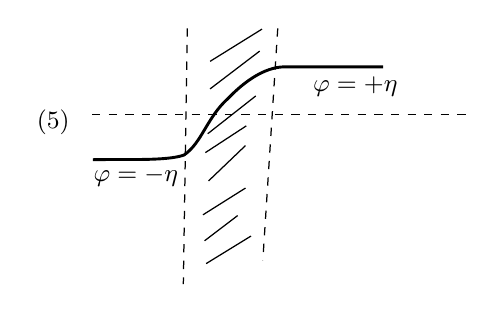
\begin{tikzpicture}[x=.010cm,y=-.010cm,font=\small,line width=.45pt]
\node[anchor=east] at (-16,119) {(5)};
\draw[dashed] (0,110)--(476,110);
\draw[dashed] (121,0)--(116,325) (236,0)--(217,295);
\draw (150,42)--(216,1) (150,77)--(213,29) (147,134)--(208,86)
      (144,158)--(196,124) (148,194)--(195,149) (141,237)--(195,203)
      (143,270)--(185,238) (145,299)--(202,264);
\draw[line width=1.05pt] (1,167)..controls(42,166)and(95,169)..(117,161)
 ..controls(140,145)and(146,113)..(173,89)
 ..controls(194,67)and(219,50)..(243,49)--(370,49);
\node[anchor=north east,inner sep=0pt] at (110,175) {$\varphi=-\eta$};
\node[anchor=north west,inner sep=0pt] at (280,61) {$\varphi=+\eta$};
\end{tikzpicture}}\endgroup
\end{center}}
\end{GelfandAdjacentEvidence}
\begin{GelfandAdjacentEvidence}{GELFAND-P001070}{8}

[To the right of the figure:] Consider a wall — \uwave{a solution localized on a plane.}
\begin{equation*}
\varphi=\varphi(x,y,z)\qquad(\text{independent of \(t\)})
\end{equation*}
\begin{equation*}
\Box\varphi+\varphi\lambda^2(\varphi^2-\eta^2)=0
\qquad\text{— Euler equation for Lagrangian (2)}
\tag{6}
\end{equation*}
\SourceFigure{GELFAND-P001070}{eq06-coefficient}{The symbol before \(\lambda^2\) is \(\varphi\).}
\end{GelfandAdjacentEvidence}
\begin{GelfandAdjacentEvidence}{GELFAND-P001070}{9}


(7) $\parallel\quad\underset{z\to\pm\infty}{\varphi=\pm\eta}$
independent of $x,y,z$ $\Rightarrow$ it is easy to verify that such a solution exists.
\SourceFigure{GELFAND-P001070}{limit-coordinate-reading}{Asymptotic condition and the manuscript’s coordinate list.}
\end{GelfandAdjacentEvidence}



\Needspace{7\baselineskip}
\begin{GelfandAdjacentEvidence}{GELFAND-P001071}{1}
\SourcePage{GELFAND-P001071}{unlabelled}
$\eta\sim m$

(8) Layer thickness [inserted below: (in (5))] $\sim\dfrac1\eta$.
\SourceFigure{GELFAND-P001071}{thickness-insertion}{Reference to (5) below the line on the layer thickness.}
\end{GelfandAdjacentEvidence}
\begin{GelfandAdjacentEvidence}{GELFAND-P001071}{2}


[illegible crossed-out mark before “Solution”\textsuperscript{?}] Solution (5) is found explicitly: \uuline{$\operatorname{th}(z\eta)$}
\Unclear{GELFAND-P001071}{before-solution05}{illegible crossed-out mark before “Solution”}
\end{GelfandAdjacentEvidence}
\begin{GelfandAdjacentEvidence}{GELFAND-P001071}{3}

\SourceFigure{GELFAND-P001071}{explicit-wall-solution}{The double-underlined \(\operatorname{th}(z\eta)\).}
\end{GelfandAdjacentEvidence}
\begin{GelfandAdjacentEvidence}{GELFAND-P001071}{4}


\dashuline{Symmetry group}: $\varphi\mapsto-\varphi$.

One now usually considers a continuous group $G$ of symmetries of the Lagrangian.
\SourceFigure{GELFAND-P001071}{continuous-symmetry}{Abbreviations in the line on the continuous group.}
\end{GelfandAdjacentEvidence}
\begin{GelfandAdjacentEvidence}{GELFAND-P001071}{5}


$U(1)$-invariant theory:
\begin{equation*}
\mathcal{L}(\varphi)=\frac12\bigl|(\partial_i+iA_i)\varphi\bigr|^2-(\varphi\varphi^*-\eta^2)^2
\tag{9}
\end{equation*}
\SourceFigure{GELFAND-P001071}{covariant-derivative-sign}{The \(+\) sign before \(iA_i\) in (9).}
\end{GelfandAdjacentEvidence}
\begin{GelfandAdjacentEvidence}{GELFAND-P001071}{6}

\begin{equation*}
\text{Vacuum: }(c_1,c_2):\quad c_1^2+c_2^2=\eta^2
\tag{10}
\end{equation*}
\SourceFigure{GELFAND-P001071}{diagram11}{%
\begin{center}
\begingroup\color{black}\GelfandFitDiagram{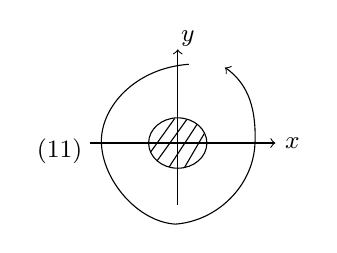
\begin{tikzpicture}[x=1cm,y=1cm,font=\small]
\node at (-1.50,-.11) {(11)};
\draw[->] (-1.12,0)--(1.24,0) node[right] {$x$};
\draw[->] (0,-.79)--(0,1.19) node[above right,inner sep=1pt] {$y$};
\draw (0,0) ellipse [x radius=.37,y radius=.32];
\begin{scope}
\clip (0,0) ellipse [x radius=.37,y radius=.32];
\draw (-.37,-.15)--(-.04,.31) (-.33,-.32)--(.13,.32)
      (-.12,-.32)--(.26,.26) (.08,-.32)--(.36,.16);
\end{scope}
\draw[->] (.14,1.00)..controls(-.55,.95)and(-.98,.45)..(-.97,.01)
 ..controls(-.96,-.47)and(-.51,-1.00)..(-.03,-1.03)
 ..controls(.50,-.99)and(.95,-.55)..(.98,-.02)
 ..controls(1.00,.41)and(.91,.74)..(.60,.96);
\end{tikzpicture}}\endgroup
\end{center}}
\end{GelfandAdjacentEvidence}
\begin{GelfandAdjacentEvidence}{GELFAND-P001071}{7}

[To the right of the figure:] A string is when the energy is concentrated along a line (one-dimensional).

On going around, the vector $C$ turns through $2\pi$

There is a topological invariant.

(Static solution: independent of $t$)

$A$ is an additional vector field (electromagnetic).
\begin{equation*}
\mathcal{L}=-\frac14F_{ik}F_{ik}+\frac12\bigl|(\partial_i+iA_i)\varphi\bigr|^2-(\varphi\varphi^*-\eta^2)^2
\tag{12}
\end{equation*}
\begin{equation*}
F_{ik}=\partial_i A_k-\partial_k A_i
\end{equation*}
Action of $U(1)$ on the field:
\begin{equation*}
\begin{cases}
\varphi\mapsto e^{i\alpha}\varphi\\
A_i\mapsto A_i+\nabla_i\alpha
\end{cases}
\tag{13}
\end{equation*}
\SourceFigure{GELFAND-P001071}{eq13-gauge-sign}{Equation (13) has \(e^{i\alpha}\) and a \(+\) sign before \(\nabla_i\alpha\).}
\end{GelfandAdjacentEvidence}
\begin{GelfandAdjacentEvidence}{GELFAND-P001071}{8}


Consider an approximate solution [crossed-out writing, possibly a number in parentheses\textsuperscript{?}]
\Unclear{GELFAND-P001071}{after-approximate-solution}{crossed-out writing, possibly a number in parentheses}
\end{GelfandAdjacentEvidence}
\begin{GelfandAdjacentEvidence}{GELFAND-P001071}{9}


\SourceFigure{GELFAND-P001071}{diagram14}{%
\begin{center}
\begingroup\color{black}\GelfandFitDiagram{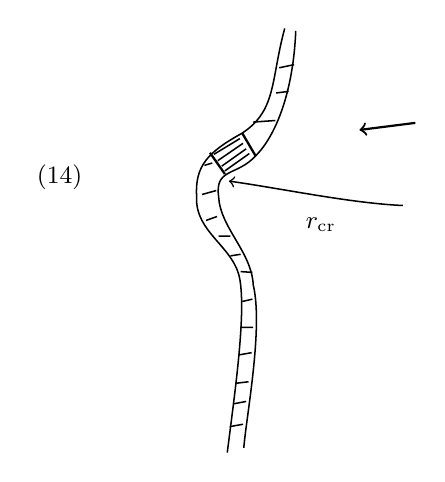
\begin{tikzpicture}[x=.010cm,y=-.010cm,font=\small,line width=.55pt]
\node at (5,189) {(14)};
\draw (291,0)..controls(273,66)and(281,104)..(237,133)
 ..controls(192,158)and(177,175)..(179,214)
 ..controls(177,260)and(227,277)..(234,319)
 ..controls(242,365)and(227,467)..(218,539);
\draw (305,3)..controls(302,80)and(280,136)..(254,162)
 ..controls(230,188)and(202,177)..(207,214)
 ..controls(209,253)and(249,284)..(251,326)
 ..controls(264,380)and(242,494)..(239,533);
\draw[line width=.83pt] (237,133)--(254,162) (196,158)--(215,185);
\draw (201,160)--(234,140) (206,168)--(238,146)
      (211,175)--(242,153) (215,181)--(246,159);
\draw (284,50)--(303,46) (280,82)--(296,80) (251,119)--(279,117)
      (189,174)--(199,171) (186,211)--(204,206) (191,244)--(205,239)
      (207,264)--(222,264) (222,289)--(235,287) (235,309)--(250,310)
      (237,347)--(250,344) (235,380)--(251,380) (232,415)--(249,412)
      (228,451)--(245,449) (226,477)--(242,474) (221,506)--(238,503);
\draw[->] (441,225)..controls(374,222)and(285,203)..(220,194);
\node at (337,249) {$r_{\mathrm{cr}}$};
\draw[->,line width=.80pt] (457,120)--(386,129);
\end{tikzpicture}}\endgroup
\end{center}
The arrow at the bend is labelled \(r_{\text{cr}}\). The strokes inside the marked section may have arrowheads.}
\end{GelfandAdjacentEvidence}
\begin{GelfandAdjacentEvidence}{GELFAND-P001071}{10}

[To the right of the figure, left arrow:] \uwave{take this as the initial condition}
\SourceFigure{GELFAND-P001071}{initial-condition-caption}{Wavy underline and singular “initial condition.”}
\end{GelfandAdjacentEvidence}
\begin{GelfandAdjacentEvidence}{GELFAND-P001071}{11}


Approximate form of solution (11):
\begin{equation*}
\begin{cases}
\varphi_1=\dfrac xr f(r)\\
\varphi_2=\dfrac yr f(r)
\end{cases}
\tag{15}
\end{equation*}
(for probably “rotation,” the first letters are only partly legible\textsuperscript{?})
\Unclear{GELFAND-P001071}{eq15-parenthesis-word}{probably “rotation,” the first letters are only partly legible}
\end{GelfandAdjacentEvidence}


[At right:] Construct $A$ in the same way.

$\varepsilon(r)$, the energy density in (11), can be calculated.


\Needspace{7\baselineskip}
\begin{GelfandAdjacentEvidence}{GELFAND-P001072}{1}
\SourcePage{GELFAND-P001072}{67}
[Crossed out: possibly “Solution (14)”\textsuperscript{?}]
\Unclear{GELFAND-P001072}{top-cancelled-reference}{possibly “Solution (14)”}
\end{GelfandAdjacentEvidence}
\begin{GelfandAdjacentEvidence}{GELFAND-P001072}{2}


They must approach the vacuum: $\varphi_1^2+\varphi_2^2\to\eta^2$ as $r\to\infty$.

Locally (14) resembles (11).

(16) Let the radius of curvature satisfy $r_{\text{cr}}\gg\dfrac1\eta$

Effective action: [arrow rightward, then down to the right side of (17)]
\begin{equation*}
S=\int\mathcal L(\varphi)\,d^4x\simeq\nu\int dl\sqrt{1-v_{\perp}^2}\,dt
\tag{17}
\end{equation*}
[Above right, arrow down-left toward the integral:] integral along the string itself.
\SourceFigure{GELFAND-P001072}{effective-action-arrows}{Two arrows to the right side of (17).}
\end{GelfandAdjacentEvidence}
\begin{GelfandAdjacentEvidence}{GELFAND-P001072}{3}

\SourceFigure{GELFAND-P001072}{action-density-symbol}{The coefficient \(\nu\) before the integral in (17).}
\end{GelfandAdjacentEvidence}
\begin{GelfandAdjacentEvidence}{GELFAND-P001072}{4}


$v_\perp$ is the transverse velocity of the string

\(\parallel\) $\nu$ is the linear energy density of the string.
\SourceFigure{GELFAND-P001072}{linear-density-key}{Double stroke and explanation of \(\nu\).}
\end{GelfandAdjacentEvidence}
\begin{GelfandAdjacentEvidence}{GELFAND-P001072}{5}


Evolution — ?

Inside the string we assume [inserted above: that] nothing happens
\SourceFigure{GELFAND-P001072}{inside-string-insertion}{“That” is inserted above the line.}
\end{GelfandAdjacentEvidence}
\begin{GelfandAdjacentEvidence}{GELFAND-P001072}{6}

(we consider its [inserted above: thickness] sufficiently small — — compared with the radii of curvature)
\SourceFigure{GELFAND-P001072}{thickness-insertion}{Insertion of “thickness” before “its.”}
\end{GelfandAdjacentEvidence}
\begin{GelfandAdjacentEvidence}{GELFAND-P001072}{7}


We evaluate the integral in each transverse section to obtain $\nu$

$\sqrt{1-v_\perp^2}$ comes from $d^4x$ (by a change of variables)

Or use relativistic invariance: $ds$ (the interval), written in any coordinate system.

(17) is the formula of \uline{Nambu}.

One can consider a ring-shaped string with Lagrangian given by the right side of (17)
\SourceFigure{GELFAND-P001072}{diagram18}{%
\begin{center}
\begingroup\color{black}\GelfandFitDiagram{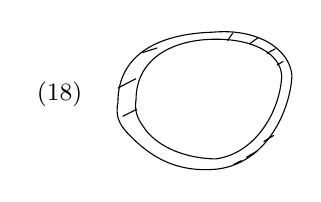
\begin{tikzpicture}[x=1cm,y=1cm,font=\small]
\node at (-1.86,.10) {(18)};
\draw (-1.12,.00)..controls(-1.12,.59)and(-.63,.87)..(.09,.89)
 ..controls(.65,.94)and(1.06,.68)..(1.09,.34)
 ..controls(1.07,-.10)and(.77,-.78)..(.13,-.85)
 ..controls(-.42,-.90)and(-.75,-.65)..(-.98,-.41)
 ..controls(-1.12,-.27)and(-1.15,-.16)..cycle;
\draw (-.89,.03)..controls(-.89,.54)and(-.45,.79)..(.09,.80)
 ..controls(.59,.81)and(.95,.62)..(.96,.33)
 ..controls(.94,-.10)and(.64,-.65)..(.12,-.72)
 ..controls(-.34,-.71)and(-.66,-.52)..(-.79,-.32)
 ..controls(-.88,-.20)and(-.91,-.10)..cycle;
\draw (-1.12,.18)--(-.89,.30) (-1.06,-.18)--(-.88,-.09)
 (-.81,.63)--(-.62,.69) (.34,.88)--(.27,.78)
 (.66,.82)--(.55,.74) (.88,.68)--(.77,.62)
 (.98,.52)--(.90,.47) (.86,-.42)--(.73,-.50)
 (.65,-.62)--(.51,-.70) (.45,-.74)--(.35,-.79);
\end{tikzpicture}}\endgroup
\end{center}}
\end{GelfandAdjacentEvidence}
\begin{GelfandAdjacentEvidence}{GELFAND-P001072}{8}

it will contract, quickly reach the speed of light, and shrink to a small lump.

\dashuline{Variant.}

break the ends (put a monopole at each):
\SourceFigure{GELFAND-P001072}{diagram19}{%
\begin{center}
\begingroup\color{black}\GelfandFitDiagram{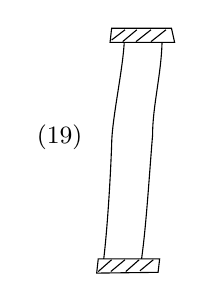
\begin{tikzpicture}[x=1cm,y=1cm,font=\small]
\node at (-1.00,.15) {(19)};
\draw (-.18,1.35)..controls(-.20,.98)and(-.34,.36)..(-.34,.04)
 ..controls(-.36,-.49)and(-.40,-1.06)..(-.44,-1.40);
\draw (.30,1.35)..controls(.29,.94)and(.18,.54)..(.18,.17)
 ..controls(.14,-.31)and(.10,-.98)..(.04,-1.40);
\draw (-.36,1.35)--(.46,1.35)--(.42,1.53)--(-.34,1.53)--cycle;
\draw (-.53,-1.58)--(.25,-1.57)--(.27,-1.40)--(-.51,-1.40)--cycle;
\draw (-.34,1.38)--(-.17,1.51) (-.20,1.36)--(-.02,1.51)
 (-.03,1.36)--(.16,1.51) (.16,1.36)--(.35,1.51)
 (-.51,-1.56)--(-.34,-1.41) (-.35,-1.56)--(-.17,-1.41)
 (-.16,-1.56)--(.01,-1.41) (.02,-1.55)--(.19,-1.41);
\end{tikzpicture}}\endgroup
\end{center}}
\end{GelfandAdjacentEvidence}
\begin{GelfandAdjacentEvidence}{GELFAND-P001072}{9}

\SourceFigure{GELFAND-P001072}{diagram20}{%
\begin{center}
\begingroup\color{black}\GelfandFitDiagram{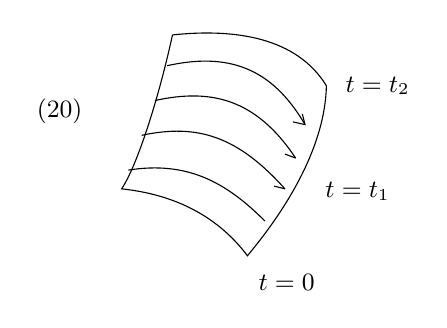
\begin{tikzpicture}[x=.017cm,y=-.017cm,font=\small]
\node[anchor=east] at (-22,57) {(20)};
\draw (38,0)..controls(85,-5)and(131,2)..(153,38)
 ..controls(152,83)and(124,129)..(94,165)
 ..controls(76,141)and(47,120)..(0,115)
 ..controls(12,97)and(28,46)..(38,0);
\draw (34,23)..controls(79,13)and(112,24)..(137,67)
 (25,49)..controls(66,40)and(100,47)..(130,92)
 (15,75)..controls(57,66)and(87,76)..(122,115)
 (5,101)..controls(49,94)and(78,110)..(107,139);
\draw (128,65)--(137,67)--(135,59)
 (122,89)--(130,92) (114,113)--(122,115);
\node[anchor=west] at (160,38) {$t=t_2$};
\node[anchor=west] at (145,117) {$t=t_1$};
\node[anchor=north west] at (95,172) {$t=0$};
\end{tikzpicture}}\endgroup
\end{center}
Short strokes are visible at the ends of three arcs. It is uncertain whether they are arrowheads.}
\end{GelfandAdjacentEvidence}
\begin{GelfandAdjacentEvidence}{GELFAND-P001072}{10}


[To the right of the figure:] As it moves, the string sweeps out a sheet.

(21) \uwave{The area of the swept surface is the Lagrangian} ($17_{\text{right}}$)
\SourceFigure{GELFAND-P001072}{swept-area-caption}{Wavy underline and reference \(17_{\text{right}}\).}
\end{GelfandAdjacentEvidence}



\Needspace{7\baselineskip}
\begin{GelfandAdjacentEvidence}{GELFAND-P001073}{1}
\SourcePage{GELFAND-P001073}{unlabelled}
$\dot x=\dfrac{\partial x}{\partial t}$, $x'=\dfrac{\partial x}{\partial s}$, $x(t,s)$ and calculate.

A $\min$ area arises.
\SourceFigure{GELFAND-P001073}{minimum-area-ending}{The Russian word after \(\min\) ends in «ь».}
\end{GelfandAdjacentEvidence}
\begin{GelfandAdjacentEvidence}{GELFAND-P001073}{2}


\uwave{Strings and chromodynamics.}

\dashuline{Quantum chromodynamics}:
\begin{equation*}
\mathcal L(\psi,A)=-\frac14F_{ik}^aF_{ik}^a+\bar\psi(i\hat\partial-m)\psi
\tag{22}
\end{equation*}
\SourceFigure{GELFAND-P001073}{eq22-field-case}{Lowercase \(\psi\) on the right side of (22).}
\end{GelfandAdjacentEvidence}
\begin{GelfandAdjacentEvidence}{GELFAND-P001073}{3}


$a=1\div8$; $i,k=0,1,2,3$.
\begin{equation*}
\hat\partial=\gamma^i(\partial_i+iI^aA_i^a)
\tag{23}
\end{equation*}
[Beneath $\gamma^i$:] Dirac matrices
\SourceFigure{GELFAND-P001073}{dirac-matrix-caption}{A short dotted stroke appears above the note beneath \(\gamma^i\).}
\end{GelfandAdjacentEvidence}
\begin{GelfandAdjacentEvidence}{GELFAND-P001073}{4}

\begin{equation*}
F_{ik}^a=\partial_i A_k^a-\partial_k A_i^a+g f_{abc}A_i^bA_k^c,
\tag{24}
\end{equation*}
$g$ is the coupling constant, and $f_{abc}$ are the structure constants of the group.

\dashuline{Acts}: the group $SU(3)$ (adjoint representation) — hence 8.

— acts on $A$

[Crossed out: illegible mark before \(I^a\), possibly \(a\)\textsuperscript{?}]
\Unclear{GELFAND-P001073}{before-generator-ia}{illegible mark before \(I^a\), possibly \(a\)}
\end{GelfandAdjacentEvidence}
\begin{GelfandAdjacentEvidence}{GELFAND-P001073}{5}


$I^a$ is a generator of $SU(3)$, $I^a=I^a_{\alpha\beta}$.

in $\bar\psi$ and $\psi$ there is also a color index (quarks are triplets) — — contraction is over that index.
\SourceFigure{GELFAND-P001073}{quark-triplet-abbreviation}{The note “quarks are triplets.”}
\end{GelfandAdjacentEvidence}
\begin{GelfandAdjacentEvidence}{GELFAND-P001073}{6}


In fact several types of quarks are needed: at least 2 types
\begin{equation*}
\mathcal L(\psi,A)=-\frac14F_{ik}^aF_{ik}^a+\bar u(i\bar\partial-m)u+\bar d(i\hat\partial-m)d
\tag{25}
\end{equation*}
\SourceFigure{GELFAND-P001073}{eq25-derivative-marks}{There is a horizontal bar over \(\partial\) in the first quark term, and a hat in the second.}
\end{GelfandAdjacentEvidence}
\begin{GelfandAdjacentEvidence}{GELFAND-P001073}{7}

[heavily overwritten symbol after the first parenthesis, provisionally \(u\)\textsuperscript{?}]
\Unclear{GELFAND-P001073}{eq25-overwritten-field}{heavily overwritten symbol after the first parenthesis, provisionally \(u\)}
\end{GelfandAdjacentEvidence}
\begin{GelfandAdjacentEvidence}{GELFAND-P001073}{8}


($u$-quarks and $d$-quarks)
\begin{equation*}
\hat\partial_i=\nabla_i+iA_i^a I^a,\qquad I^a=I^a_{\alpha\beta}
\tag{26}
\end{equation*}
$A$ is a Yang–Mills field, or a \uline{gluon field} (it glues quarks together)

(gluon field)
\SourceFigure{GELFAND-P001073}{gluon-caption}{English “gluon field” beneath the underlined word.}
\end{GelfandAdjacentEvidence}



\clearpage\pdfbookmark[0]{Chapter 23}{gelfand-archive-chapter-23}
\section*{Chapter 23}


\Needspace{7\baselineskip}
\begin{GelfandAdjacentEvidence}{GELFAND-P001074}{1}
\SourcePage{GELFAND-P001074}{1}
\uline{7/II–83}

\uuline{Gelfand Seminar}

\uline{I. M. G.} There is no familiar understanding of the $\infty$-dimensional symplectic group,
$\infty$-dim. [inserted above: sympl.]
\Unclear{GELFAND-P001074}{top-abbreviation}{abbreviation apparently for “geometry,” ending indistinct}
\end{GelfandAdjacentEvidence}
\begin{GelfandAdjacentEvidence}{GELFAND-P001074}{2}

and so on. “Fock space is a toy for mathematicians.”

There are popular lectures by Witten on supermathematics! (preprint; lectures)
\begin{equation*}
\begin{gathered}
\downarrow\\
\text{The Atiyah–Bott theorem follows from super considerations}\\
\text{(on fixed points)}
\end{gathered}
\end{equation*}
\SourceFigure{GELFAND-P001074}{witten-annotation}{Arrow from Witten’s lectures to the Atiyah–Bott theorem.}
\end{GelfandAdjacentEvidence}
\begin{GelfandAdjacentEvidence}{GELFAND-P001074}{3}


\uline{Kirillov on Neretin’s work}
\begin{equation*}
T(g)f(z)=f\left(\frac{\alpha z+\gamma}{\beta z+\delta}\right)
|\beta z+\delta|^\lambda
\end{equation*}
The representation of $SL(2,\mathbb R)$ extends to a representation of $\operatorname{Diff}(S^1)$ (unitarily!).
\begin{equation*}
f\longmapsto f(\varphi^{-1}(z))
\left|\frac{d\varphi^{-1}(z)}{dz}\right|^{-\lambda/2}
\end{equation*}
[At left with a brace:] this is nonunitary, but
\SourceFigure{GELFAND-P001074}{nonunitary-margin}{Annotation and brace before “from this.”}
\end{GelfandAdjacentEvidence}
\begin{GelfandAdjacentEvidence}{GELFAND-P001074}{4}

from this, unitary representations are constructed (by considering the action in Fock space —
\SourceFigure{GELFAND-P001074}{margin-upper-parenthesis}{Separate closing parenthesis at the right of the line.}
\end{GelfandAdjacentEvidence}
\begin{GelfandAdjacentEvidence}{GELFAND-P001074}{5}


— on coherent states.
\SourceFigure{GELFAND-P001074}{coherent-states}{Abbreviation for “coherent” before “states.”}
\end{GelfandAdjacentEvidence}
\begin{GelfandAdjacentEvidence}{GELFAND-P001074}{6}


Idea:
\begin{equation*}
\operatorname{Im}\int f(x_1)\overline{g(x_2)}
\frac{|x_1-x_2|^{-2+\lambda}}{\Gamma(-1+\lambda)}\,dx_1\,dx_2
\qquad\text{(symplectic form!)}
\end{equation*}
\uwave{preserved under fractional linear transformations}
[crossed-out arrow \(\rightarrow\)?]
\Unclear{GELFAND-P001074}{crossed-arrow}{crossed-out mark resembling a right arrow}
\end{GelfandAdjacentEvidence}
\begin{GelfandAdjacentEvidence}{GELFAND-P001074}{7}

$\Rightarrow$ not preserved under all diffeomorphisms, but of similar form.

\SourceFigure{GELFAND-P001074}{unitary-group-annotation}{%
\begin{center}
\begingroup\color{black}\GelfandFitDiagram{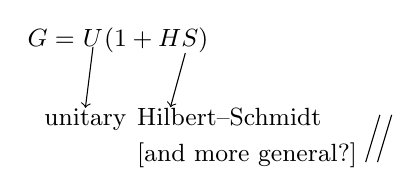
\begin{tikzpicture}[font=\small,x=1cm,y=1cm]
\node[anchor=base west,inner sep=0pt] (group) at (0,0) {$G={}$};
\node[anchor=base west,inner sep=0pt] (unitary) at (group.base east) {$U$};
\node[anchor=base west,inner sep=0pt] (sum) at (unitary.base east) {$(1+HS)$};
\node[anchor=base,inner sep=0pt] (unitarylabel) at (.74,-1.0) {unitary};
\node[anchor=base west,inner sep=0pt] (hslabel) at (1.39,-1.0) {Hilbert–Schmidt};
\draw[->] (unitary.south)--(unitarylabel.north);
\draw[->] ([xshift=-.30cm]sum.south east)--([xshift=.43cm]hslabel.north west);
\node[anchor=base west,inner sep=0pt] at (1.39,-1.46) {[and more general?]};
\draw (4.30,-1.47)--(4.48,-.87) (4.45,-1.47)--(4.63,-.87);
\end{tikzpicture}}\endgroup
\end{center}
The bottom annotation is provisional. Two oblique strokes appear at right.}
\end{GelfandAdjacentEvidence}
\begin{GelfandAdjacentEvidence}{GELFAND-P001074}{8}


\uline{B. Feigin.}

\dashuline{Strings and representations of $\operatorname{Diff}S^1$.}

$V$ is the space of maps $S^1\longrightarrow\mathbb R^d$. A metric is given on $\mathbb R^d$ (Riemannian or Lorentzian).
$\operatorname{Diff}S^1$ acts (changes of parameter).
\begin{equation*}
f,g\longmapsto\int_{S^1}(f,dg)
\tag{1}
\end{equation*}
On $V/V_{\mathrm{const}}$ one obtains a nondegenerate form. Put $V'=V/V_{\mathrm{const}}$.
[Below $V_{\mathrm{const}}$:] constant maps.
\SourceFigure{GELFAND-P001074}{constant-map-caption}{Stroke from $V_{\mathrm{const}}$ toward its caption.}
\end{GelfandAdjacentEvidence}
\begin{GelfandAdjacentEvidence}{GELFAND-P001074}{9}


On $\underbrace{V'/\operatorname{Diff}S^1}$ there is a Hamiltonian structure (Poisson bracket).

\dashuline{Problem}: quantize this situation.
[marginal stroke]
\Unclear{GELFAND-P001074}{margin-lower-mark}{short oblique mark before a closing parenthesis in the right margin}
\end{GelfandAdjacentEvidence}
\begin{GelfandAdjacentEvidence}{GELFAND-P001074}{10}


\dashuline{Kirillov.} $M$ is a symplectic manifold. $G$ is a group acting on $M$ and preserving its symplectic structure. $\Rightarrow$ One constructs the reduced manifold $M_{\mathrm{red}}$ (symplectic reduction).

idea: $\{\ \}$ on invariant functions is degenerate. One must take a quotient.

\uline{B. F.} $V'$ is a space with a nondegenerate symplectic form.
The quantization method is to choose $p,q$ and realize them in the usual way (Fock space).
In finite dimension this is a satisfactory method. Where does it act? The space of invariants.
The $\infty$-dimensional case is problematic.
The representation of the symplectic manifold\textsuperscript{?} is projective, and invariants do not exist. The space must be changed.
\Unclear{GELFAND-P001074}{last-line-subject}{abbreviation provisionally read as «мн.» (“manifold”)}
\end{GelfandAdjacentEvidence}
\begin{GelfandAdjacentEvidence}{GELFAND-P001074}{11}

(a Schwinger term appears)
\SourceFigure{GELFAND-P001074}{bottom-parenthesis}{Small note on the Schwinger term below the last line.}
\end{GelfandAdjacentEvidence}



\Needspace{7\baselineskip}
\begin{GelfandAdjacentEvidence}{GELFAND-P001075}{1}
\SourcePage{GELFAND-P001075}{unlabelled}
$\operatorname{sp}(V')$ is the Lie algebra of symplectic transformations.

$\mathcal L$ is the algebra of vector fields on $S^1$.

\SourceFigure{GELFAND-P001075}{representation-diagram}{%
\begin{center}
\begingroup\color{black}\GelfandFitDiagram{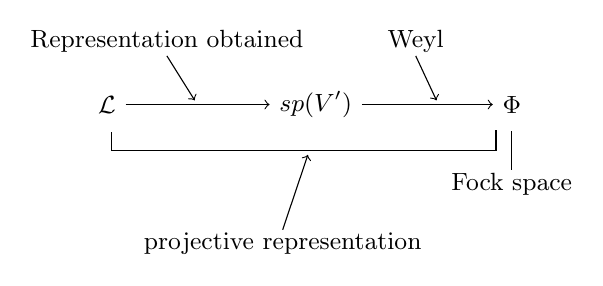
\begin{tikzpicture}[font=\small,x=1cm,y=1cm]
\node (ell) at (0,0) {$\mathcal L$};
\node (sp) at (2.65,0) {$\operatorname{sp}(V')$};
\node (fock) at (5.14,0) {$\Phi$};
\draw[->] (ell.east)--(sp.west) coordinate[pos=.48] (first);
\draw[->] (sp.east)--(fock.west) coordinate[pos=.57] (second);
\node[inner sep=1pt] (firstlabel) at (.76,.80) {Representation obtained};
\node[inner sep=1pt] (secondlabel) at (3.92,.80) {Weyl};
\draw[->] (firstlabel.south)--([yshift=1.5pt]first);
\draw[->] (secondlabel.south)--([yshift=1.5pt]second);
\draw (.06,-.35)--(.06,-.58)--(4.94,-.58)--(4.94,-.33);
\node[anchor=north,align=center,inner sep=1pt] (focklabel) at (5.14,-.83) {Fock space};
\draw (5.14,-.34)--(focklabel.north);
\node[inner sep=1pt] (projective) at (2.23,-1.77) {\dashuline{projective} representation};
\draw[->] (projective.north)--(2.55,-.64);
\end{tikzpicture}}\endgroup
\end{center}
The label above the second arrow reads “Weyl.”}
\end{GelfandAdjacentEvidence}
\begin{GelfandAdjacentEvidence}{GELFAND-P001075}{2}


$\Phi$ is constructed as follows:

$V'$, [crossed out]
\Unclear{GELFAND-P001075}{cancel-after-v}{the crossed-out mark after \(V'\) is illegible}
\end{GelfandAdjacentEvidence}
\begin{GelfandAdjacentEvidence}{GELFAND-P001075}{3}

$S^1\longrightarrow\mathbb R^d$.

complexify and decompose
\begin{equation*}
\begin{array}{rcccl}
V'={}&H^+&\oplus&H^-&\\
&\vert&&\vert&\\
&\text{(annihilation operators)}&\leftrightarrow&\text{(creation operators)}&
\end{array}
\qquad
\Phi=\bigoplus S^i H_+.
\end{equation*}
\SourceFigure{GELFAND-P001075}{fock-decomposition}{Decomposition of \(V'\), operator labels and formula for \(\Phi\).}
\end{GelfandAdjacentEvidence}
\begin{GelfandAdjacentEvidence}{GELFAND-P001075}{4}


$H^+$ consists of functions analytic inside.
[faint mark in the margin]
\Unclear{GELFAND-P001075}{faint-right-trace}{a faint broken trace at the right of the line with no legible letters}
\end{GelfandAdjacentEvidence}
\begin{GelfandAdjacentEvidence}{GELFAND-P001075}{5}


\begin{center}\rule{1.55em}{.45pt}\enspace\(\cdot\)\enspace\rule{1.55em}{.45pt}\end{center}
\begin{equation*}
\mathcal L=\{L_i,c\},\quad i\in\mathbb Z.
\end{equation*}
\begin{equation*}
[L_i,L_j]=(j-i)L_{i+j}+
\underbrace{\delta_{i,-j}\frac{i^3-i}{12}\,c}_{\text{Schwinger term}}.
\end{equation*}
\SourceFigure{GELFAND-P001075}{schwinger-label}{Bracket and caption beneath the central term.}
\end{GelfandAdjacentEvidence}
\begin{GelfandAdjacentEvidence}{GELFAND-P001075}{6}


$\phi^{L_+}$ is the space of invariants for the subalgebra $L_+$, and there is a map.
\begin{equation*}
\begin{aligned}
L_+&=\{\text{[crossed out]}\ L_1,L_2,\ldots\},\\
L_-&=\{L_{-1},L_{-2},\ldots\}.
\end{aligned}
\end{equation*}
\Unclear{GELFAND-P001075}{cancelled-generator}{heavily crossed out before \(L_1\), possibly \(L_0\)}
\end{GelfandAdjacentEvidence}
\begin{GelfandAdjacentEvidence}{GELFAND-P001075}{7}


\SourceFigure{GELFAND-P001075}{invariant-image-diagram}{%
\begin{center}
\begingroup\color{black}\GelfandFitDiagram{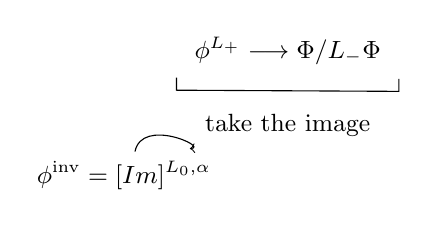
\begin{tikzpicture}[font=\small,x=1cm,y=1cm]
\node (map) at (3.00,0) {$\phi^{L_+}\longrightarrow\Phi/L_-\Phi$};
\draw ([xshift=-3pt,yshift=-1pt]map.south west) -- ++(0,-.16)
      -- ([xshift=3pt,yshift=-.21cm]map.south east) -- ++(0,.16);
\node (caption) at (3.00,-.94) {take the \uuline{image}};
\node (inv) at (.92,-1.58) {$\phi^{\mathrm{inv}}=[\operatorname{Im}]^{L_0,\alpha}$};
\draw[->] ([xshift=4pt]inv.north) .. controls (1.15,-.84) and (1.99,-1.22) ..
          ([xshift=-2pt,yshift=-1pt]caption.south west);
\end{tikzpicture}}\endgroup
\end{center}}
\end{GelfandAdjacentEvidence}


Nontrivial at least when \uline{$d=26$}.

\dashuline{Problem} (I. M. G.). Construct a $p$-adic analogue of the representation of the diffeomorphism group.


\Needspace{7\baselineskip}
\begin{GelfandAdjacentEvidence}{GELFAND-P001076}{1}
\SourcePage{GELFAND-P001076}{unlabelled}
\uuline{14/II–83}\qquad\uline{Gelfand Seminar.}

\uline{Yu. Neretin.}
\SourceFigure{GELFAND-P001076}{neretin-heading}{Date and speaker’s name.}
\end{GelfandAdjacentEvidence}
\begin{GelfandAdjacentEvidence}{GELFAND-P001076}{2}


$\forall\rho$ almost preserves the inner product.
\begin{equation*}
\frac{1}{\Gamma(\rho)}\int_{-\infty}^{\infty}
|x_1-x_2|^{-\rho}f(x_1)\overline{g(x_2)}\,dx_1\,dx_2.
\tag{1}
\end{equation*}
([crossed out] the operator will be \uuline{$O(1+T)$}.)
\Unclear{GELFAND-P001076}{upper-cancel}{illegible crossed-out writing before “operator”}
\end{GelfandAdjacentEvidence}
\begin{GelfandAdjacentEvidence}{GELFAND-P001076}{3}

[Below \(T\), a vertical stroke to the annotation:] \uuline{H.–S}.
\SourceFigure{GELFAND-P001076}{hilbert-schmidt-annotation}{Double underlines and annotation for \(T\).}
\end{GelfandAdjacentEvidence}
\begin{GelfandAdjacentEvidence}{GELFAND-P001076}{4}


Hilbert transform:
\begin{equation*}
Hf(s)=\frac{1}{2\pi}\int_0^{2\pi}
\operatorname{ctg}\left(\frac{t-s}{2}\right)f(t)\,dt
\qquad\text{($f$ is a real function)}
\tag{2}
\end{equation*}
\begin{equation*}
H:\mathrm{const}\longrightarrow0
\end{equation*}
$\rho=0,2\quad\Rightarrow$ in the space modulo $\mathrm{const}$ or with $\int=0$.

$H$ introduces a complex structure.

In Fourier modes:
\begin{equation*}
\parallel\quad
\begin{aligned}
\cos n\varphi&\longrightarrow-\sin n\varphi\\
\sin n\varphi&\longrightarrow\cos n\varphi
\end{aligned}
\end{equation*}
\SourceFigure{GELFAND-P001076}{fourier-annotation}{Double stroke to the left of the two lines and overwritten \(n\) in the second.}
\end{GelfandAdjacentEvidence}
\begin{GelfandAdjacentEvidence}{GELFAND-P001076}{5}


\uwave{Inner product}
\begin{equation*}
\int\ln\left|\sin\frac{t-s}{2}\right|f_1(t)f_2(s)\,dt\,ds
\end{equation*}
\begin{equation*}
\int\text{[crossed out]}\ \operatorname{ctg}\left(\frac{t-s}{2}\right)f_1(t)f'_2(s)\,dt\,ds
\end{equation*}
\Unclear{GELFAND-P001076}{integrand-cancel}{heavily crossed-out writing after the integral sign, possibly beginning with \(\ln\)}
\end{GelfandAdjacentEvidence}
\begin{GelfandAdjacentEvidence}{GELFAND-P001076}{6}


$\Rightarrow$ $H$ defines a complex structure.
\Unclear{GELFAND-P001076}{lower-cancel}{illegible crossed-out writing between the arrow and \(H\)}
\end{GelfandAdjacentEvidence}
\begin{GelfandAdjacentEvidence}{GELFAND-P001076}{7}


[At right:] by decomposition into analytic and antianalytic functions
\SourceFigure{GELFAND-P001076}{analytic-margin-arrow}{Arrow down from the right-hand note to the remark on Hermitian extension.}
\end{GelfandAdjacentEvidence}
\begin{GelfandAdjacentEvidence}{GELFAND-P001076}{8}

$\Rightarrow$ take the Hermitian extension using this $H$.
\SourceFigure{GELFAND-P001076}{hermitian-separator}{Hatched double stroke at the left of the arrow.}
\end{GelfandAdjacentEvidence}
\begin{GelfandAdjacentEvidence}{GELFAND-P001076}{9}


$\operatorname{Im}\langle\cdot\,;\,\cdot\rangle$
\uwave{is preserved under all diffeomorphisms}.
\SourceFigure{GELFAND-P001076}{all-diffeomorphisms-emphasis}{Mark above “all” and wavy underlining.}
\end{GelfandAdjacentEvidence}
\begin{GelfandAdjacentEvidence}{GELFAND-P001076}{10}


\uline{I. M. G.}\quad\uline{Problem:} make this a general statement about pseudodifferential operators!!
(invariant under [inserted above: all] diffeomorphisms!!)
\SourceFigure{GELFAND-P001076}{all-insertion}{“All” is inserted above the line.}
\end{GelfandAdjacentEvidence}



\Needspace{7\baselineskip}
\begin{GelfandAdjacentEvidence}{GELFAND-P001077}{1}
\SourcePage{GELFAND-P001077}{unlabelled}
\dashuline{Symplectic form} — ?

Yu. N.\quad\uwave{Projections}: $H\pm i$
\SourceFigure{GELFAND-P001077}{projector-normalization}{The manuscript reads \(H\pm i\).}
\end{GelfandAdjacentEvidence}
\begin{GelfandAdjacentEvidence}{GELFAND-P001077}{2}


\dashuline{their images}: \dashuline{Lagrangian manifolds}.

Symplectic form:
\begin{equation*}
\{f_1,f_2\}=\langle f_1,Hf_2\rangle
\end{equation*}
\uuline{I. M. G.} [crossed out]
\Unclear{GELFAND-P001077}{cancel-after-img}{illegible crossed-out writing after the initials}
\end{GelfandAdjacentEvidence}
\begin{GelfandAdjacentEvidence}{GELFAND-P001077}{3}

[Inserted above: “We must also.”] consider a generalization of $c[1+(\text{comp.})]$
($\Rightarrow$ write the whole series in symbols).
\SourceFigure{GELFAND-P001077}{img-insertion}{“We must also” is inserted above the line.}
\end{GelfandAdjacentEvidence}
\begin{GelfandAdjacentEvidence}{GELFAND-P001077}{4}


[Crossed-out formula: \(\iint\ln\left|\sin\frac{t-s}{2}\right|\).]
\SourceFigure{GELFAND-P001077}{cancelled-log-kernel}{Crossed-out formula containing \(\sin\).}
\end{GelfandAdjacentEvidence}
\begin{GelfandAdjacentEvidence}{GELFAND-P001077}{5}


\uuline{Claim}
\begin{equation*}
\iint\ln\left|\frac{t-s}{2}\right|f_1(t)f_2(\sigma)
\frac{1}{s-\sigma}\,ds\,d\sigma\,dt
\end{equation*}
\Unclear{GELFAND-P001077}{corrected-denominator}{denominator corrected. \(s-\sigma\) is written below. The cancelled beginning resembles \(t-\)}
\end{GelfandAdjacentEvidence}
\begin{GelfandAdjacentEvidence}{GELFAND-P001077}{6}

\Unclear{GELFAND-P001077}{corrected-differential}{a symbol after \(d\) is crossed out before \(\sigma\), possibly \(t\)}
\end{GelfandAdjacentEvidence}
\begin{GelfandAdjacentEvidence}{GELFAND-P001077}{7}


\uwave{is preserved under diffeomorphisms}

$\Rightarrow$ must be a differential operator ($f'$).

\dashuline{Need}: to calculate:
\begin{equation*}
\int\ln\left|\frac{t-s}{2}\right|\frac{1}{s-\sigma}\,ds.
\end{equation*}
We should obtain $\delta'$.
\SourceFigure{GELFAND-P001077}{delta-prime-claim}{The manuscript reads \(\delta'\).}
\end{GelfandAdjacentEvidence}
\begin{GelfandAdjacentEvidence}{GELFAND-P001077}{8}


We must continue analytically!!
\begin{equation*}
\int_{-\infty}^{\infty}|x|^\lambda f(x)\,dx
=\int_{|x|<1}+\int_{|x|>1}
\end{equation*}
\Unclear{GELFAND-P001077}{split-integral-limits}{marks resembling \(\infty\) are crossed out above both integrals on the right. The mark beneath the second may have been \(-\infty\)}
\end{GelfandAdjacentEvidence}
\begin{GelfandAdjacentEvidence}{GELFAND-P001077}{9}

and we continue each analytically.

Idea:
\begin{equation*}
\int|t-s|^\lambda\ \ldots
\end{equation*}
\uwave{and differentiate with respect to $\lambda$}!!

\begin{center}\rule{1.55em}{.45pt}\enspace\(\cdot\)\enspace\rule{1.55em}{.45pt}\end{center}
\uuline{\sout{V. Ginzburg}}
\SourceFigure{GELFAND-P001077}{ginzburg-cancellation}{Crossed-out name with a double underline.}
\end{GelfandAdjacentEvidence}
\begin{GelfandAdjacentEvidence}{GELFAND-P001077}{10}

\uwave{Another problem (following Feigin!):}

How does a diffeomorphism of $S^1$ act on a sequence of analytic functions
\begin{equation*}
\{f_1(z),f_2(z_1,z_1),f_3(z_1,z_2,z_3),\ldots\}
\end{equation*}
\Unclear{GELFAND-P001077}{f2-second-argument-subscript}{the second subscript in \(f_2\) looks more like 1. It may be 2}
\end{GelfandAdjacentEvidence}
\begin{GelfandAdjacentEvidence}{GELFAND-P001077}{11}

$|z|<1$.

What effect does smoothness have?

For $\varphi$ fractional linear, this coincides with the usual one!
\Unclear{GELFAND-P001077}{fractional-map-symbol}{overwritten mark before “fractional linear,” provisionally \(\varphi\)}
\end{GelfandAdjacentEvidence}


How can this be realized?


\Needspace{7\baselineskip}
\begin{GelfandAdjacentEvidence}{GELFAND-P001078}{1}
\SourcePage{GELFAND-P001078}{5}
\uuline{V. Ginzburg.}

On the work of \uwave{Duistermaat, Heckman} (Invent. Math., 1982)
\SourceFigure{GELFAND-P001078}{ginzburg-citation}{Speaker’s name and the authors of the work.}
\end{GelfandAdjacentEvidence}
\begin{GelfandAdjacentEvidence}{GELFAND-P001078}{2}


$T=\mathbb T^k$ is a torus ($k$-dimensional). $M$ is a compact symplectic manifold.
$T$ acts on $M$ in a Hamiltonian way: it preserves the symplectic structure and every vector field
\Unclear{GELFAND-P001078}{action-cancel}{crossed out, possibly «не» or «на»}
\end{GelfandAdjacentEvidence}
\begin{GelfandAdjacentEvidence}{GELFAND-P001078}{3}

from the Lie algebra of $T$ determines a field given by a Hamiltonian, and these Hamiltonians commute (with respect to the Poisson bracket).
\SourceFigure{GELFAND-P001078}{hamiltonian-phrase}{The Russian text reads “a field given.”}
\end{GelfandAdjacentEvidence}
\begin{GelfandAdjacentEvidence}{GELFAND-P001078}{4}


(Commuting fields do not imply commuting functions.)

(This is now called a Poisson Hamiltonian action.)

[At left, beyond the double stroke:] A map arises:
\SourceFigure{GELFAND-P001078}{moment-map-diagram}{%
\begin{center}
\begingroup\color{black}\GelfandFitDiagram{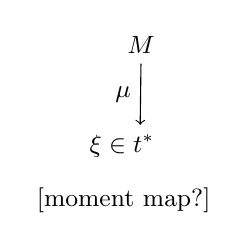
\begin{tikzpicture}[font=\small,x=1cm,y=1cm]
\node (manifold) at (.24,.8) {$M$};
\node (dual) at (0,-.48) {$\xi\in t^*$};
\draw[->] (manifold.south)--([xshift=.23cm]dual.north) node[midway,left] {$\mu$};
\node[anchor=north] at (.02,-.89) {[moment map?]};
\end{tikzpicture}}\endgroup
\end{center}
The caption beneath the diagram is faint. The end of the abbreviation is indistinct.}
\end{GelfandAdjacentEvidence}
\begin{GelfandAdjacentEvidence}{GELFAND-P001078}{5}


Or: give functions $f_1,\ldots,f_k$: \uuline{$\{f_i,f_j\}=0$}, \uwave{The flows of $f_i$ are periodic}.
\Unclear{GELFAND-P001078}{functions-mark}{mark over the end of the abbreviation “functions,” resembling an asterisk or a correction}
\end{GelfandAdjacentEvidence}
\begin{GelfandAdjacentEvidence}{GELFAND-P001078}{6}


\dashuline{Local condition}: \uwave{the fields lie in one Lagrangian}
\Unclear{GELFAND-P001078}{local-cancel}{crossed-out word beginning “sub…,” probably “subspace”}
\end{GelfandAdjacentEvidence}
\begin{GelfandAdjacentEvidence}{GELFAND-P001078}{7}

\uwave{subspace at every point}.

[crossed-out heading]
\Unclear{GELFAND-P001078}{cancelled-heading}{crossed-out heading, possibly “Next” or “Another”}
\end{GelfandAdjacentEvidence}
\begin{GelfandAdjacentEvidence}{GELFAND-P001078}{8}

\begin{equation*}
\mu(m)(X)=H_X(m)\qquad\text{($X$ is any field)}
\tag{1}
\end{equation*}
\SourceFigure{GELFAND-P001078}{moment-map-x}{The \(X\) in the argument of \(\mu(m)\) is retraced.}
\end{GelfandAdjacentEvidence}
\begin{GelfandAdjacentEvidence}{GELFAND-P001078}{9}


Or: \uwave{The cocycle} $X_1,X_2\longrightarrow\omega(X_1,X_2)(m)$
on the Lie algebra must be trivial.

\uline{Example}: $\{y,-x\}$ give commuting fields
$\dfrac{\partial}{\partial x}$, $\dfrac{\partial}{\partial y}$,
but their bracket is $\ne0$.

\begin{equation*}
M_\xi=\mu^{-1}(\xi)\quad\text{; on it \(\omega\) is degenerate;}
\tag{2}
\end{equation*}
On $M_\xi/T$ [inserted above: “it”] is already nondegenerate.
\SourceFigure{GELFAND-P001078}{reduced-form-insertion}{“It” is inserted above the line.}
\end{GelfandAdjacentEvidence}
\begin{GelfandAdjacentEvidence}{GELFAND-P001078}{10}

Denote it by $\omega_\xi$. One can calculate volume with respect to it.

\uline{Statement of the lemma}: $\omega_\xi$ is [inserted above: “piecewise”] linear in $\xi$ ($\mathrm{mod}$ exact differentials).
\SourceFigure{GELFAND-P001078}{piecewise-insertion}{Insertion of the abbreviation for “piecewise” before “linear.”}
\end{GelfandAdjacentEvidence}
\begin{GelfandAdjacentEvidence}{GELFAND-P001078}{11}


\uline{Corollary.} $\operatorname{vol}(M_\xi)$ is piecewise polynomial.
\SourceFigure{GELFAND-P001078}{reduced-volume-notation}{The notation is \(\operatorname{vol}(M_\xi)\).}
\end{GelfandAdjacentEvidence}
\begin{GelfandAdjacentEvidence}{GELFAND-P001078}{12}


(3)\quad\uline{Theorem.} Consider a vector $X\in t$ and the corresponding Hamiltonian $H_X$
\SourceFigure{GELFAND-P001078}{lie-algebra-annotation}{The abbreviation for “Lie algebra” appears beneath \(t\).}
\end{GelfandAdjacentEvidence}
\begin{GelfandAdjacentEvidence}{GELFAND-P001078}{13}

(the lift of $X$ as a function on $t^*$ using $\mu$). Then the integral
\begin{equation*}
\int_M e^{iH_X(m)}\,dm
\tag{4}
\end{equation*}
(a function on the Lie algebra)

can be calculated by stationary phase, and this gives an exact answer.

Answer:
\begin{equation*}
\int_M e^{iH_X(m)}\,dm
=\sum_j\frac{\operatorname{vol}(M_j)e^{iH_X(M_j)}}
{\prod_k\lambda_{jk}(X)}
\tag{5}
\end{equation*}
\SourceFigure{GELFAND-P001078}{localization-formula}{Equation (5), with \(\operatorname{vol}(M_j)\) and a product in the denominator.}
\end{GelfandAdjacentEvidence}
\begin{GelfandAdjacentEvidence}{GELFAND-P001078}{14}


The fixed points of $X$ (= stationary points) form a symplectic submanifold (possibly disconnected).
$M_j$ are its connected components. The $\lambda_{jk}(X)$ are linear forms that are computed
(Jacobian of the action in transverse directions).
\SourceFigure{GELFAND-P001078}{bottom-parenthesis}{The bottom parenthesis reads “Jacobian of the action in transverse directions.”}
\end{GelfandAdjacentEvidence}



\Needspace{7\baselineskip}
\begin{GelfandAdjacentEvidence}{GELFAND-P001079}{1}
\SourcePage{GELFAND-P001079}{unlabelled}
\uwave{Atiyah, Bott}\quad\dashuline{generalized and improved it}.

\uwave{M. Vergne} — something else on the subject (Michèle Vergne).
\SourceFigure{GELFAND-P001079}{scholarly-names}{Atiyah, Bott, and Vergne in the manuscript.}
\end{GelfandAdjacentEvidence}
\begin{GelfandAdjacentEvidence}{GELFAND-P001079}{2}


An old result of \uwave{Atiyah} and \uwave{Guillemin–Sternberg}:
the image of $\mu$ — is a convex region!!

(5) $\sim$ Weyl’s character formula.

($\sim10$ years ago there was a paper by Semenov-Tian-Shansky with similar content.)
\SourceFigure{GELFAND-P001079}{semenov-citation}{Reference to the paper by Semenov-Tian-Shansky.}
\end{GelfandAdjacentEvidence}
\begin{GelfandAdjacentEvidence}{GELFAND-P001079}{3}


\uline{Idea of the proof}: by stationary phase
\begin{equation*}
\int_M e^{itH_X(m)}\,dm
=\sum\frac{\operatorname{vol}(M_j)e^{itH_X(M_j)}}
{\prod_k\lambda_{jk}(X)}+\text{lower-order terms}
\end{equation*}
\SourceFigure{GELFAND-P001079}{stationary-phase-parameter}{The parameter $t$ in the exponents. The denominator reads $\prod_k\lambda_{jk}(X)$.}
\end{GelfandAdjacentEvidence}
\begin{GelfandAdjacentEvidence}{GELFAND-P001079}{4}


Locally quadratic $\Rightarrow$ the remainder is a rapidly decaying function.

Piecewise polynomial $\Rightarrow$ exponentials and polynomials $\Rightarrow$ remainder $=0$.

\dashuline{Connection with representation theory}:
\SourceFigure{GELFAND-P001079}{coadjoint-orbit-diagram}{%
\begin{center}
\begingroup\color{black}\GelfandFitDiagram{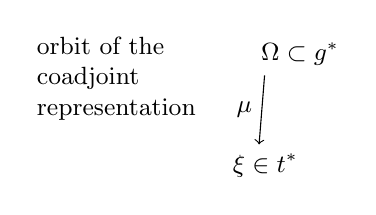
\begin{tikzpicture}[font=\small]
\node[align=left,anchor=east] at (-.55,.39) {orbit of the\\coadjoint\\representation};
\node (orbit) at (.65,.7) {$\Omega\subset g^*$};
\node (point) at (.21,-.72) {$\xi\in t^*$};
\draw[->] ([xshift=-.45cm]orbit.south)--([xshift=-.08cm]point.north)
node[midway,left] {$\mu$};
\end{tikzpicture}}\endgroup
\end{center}
}
\end{GelfandAdjacentEvidence}
\begin{GelfandAdjacentEvidence}{GELFAND-P001079}{5}

\Unclear{GELFAND-P001079}{coadjoint-target-cancel}{illegible crossed-out notation before $t^*$}
\end{GelfandAdjacentEvidence}
\begin{GelfandAdjacentEvidence}{GELFAND-P001079}{6}


$G$ compact $\Rightarrow\Omega$ compact.

We obtain the Harish-Chandra integral.

Kirillov: this is — \uwave{the character}.

\uwave{M. Vergne}: proof for noncompact orbits of the discrete series.

\uuline{A. A. Kirillov.}

$SU(3)$\qquad $H_0(3)\supset\Omega$

acts on Hermitian matrices (of trace $0$), an $8$-dimensional manifold
\[
h\longrightarrow ghg^{-1}
\]
\SourceFigure{GELFAND-P001079}{conjugation-display}{The conjugation formula.}
\end{GelfandAdjacentEvidence}
\begin{GelfandAdjacentEvidence}{GELFAND-P001079}{7}


Orbit $\Omega$: $2$ invariants $\operatorname{Sp}(A^2)$, $\operatorname{Sp}(A^3)$.
[Below «Orbit»: «6-dimensional».]
\SourceFigure{GELFAND-P001079}{orbit-dimension-annotation}{The handwritten note on the orbit dimension.}
\end{GelfandAdjacentEvidence}
\begin{GelfandAdjacentEvidence}{GELFAND-P001079}{8}

\SourceFigure{GELFAND-P001079}{orbit-projection-map}{%
\begin{center}
\begingroup\color{black}\GelfandFitDiagram{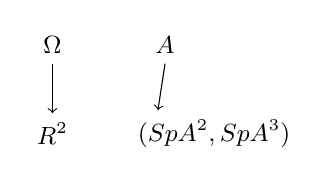
\begin{tikzpicture}[font=\small]
\node (o) at (-.86,.56) {$\Omega$};
\node (r) at (-.86,-.56) {$\mathbb R^2$};
\node (a) at (.57,.56) {$A$};
\node[anchor=west] (t) at (.1,-.56) {$(\operatorname{Sp}A^2,\operatorname{Sp}A^3)$};
\draw[->] (o)--(r);
\draw[->] (a.south)--([xshift=.38cm]t.north west);
\end{tikzpicture}}\endgroup
\end{center}
}
\end{GelfandAdjacentEvidence}
\begin{GelfandAdjacentEvidence}{GELFAND-P001079}{9}


The projection of $\Omega$ onto $\mathbb R^2$ — is an almost regular hexagon.

\SourceFigure{GELFAND-P001079}{hexagon-diagram}{%
\begin{center}
\begingroup\color{black}\GelfandFitDiagram{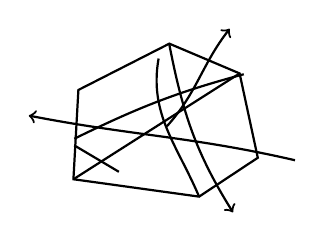
\begin{tikzpicture}[x=1.05cm,y=1.05cm,thick]
\coordinate (a) at (-1.11,-.67);
\coordinate (b) at (-1.05,.41);
\coordinate (c) at (.05,.97);
\coordinate (d) at (.9,.61);
\coordinate (e) at (1.12,-.41);
\coordinate (f) at (.41,-.88);
\draw (a)--(b)--(c)--(d)--(e)--(f)--cycle;
\draw (a)--(d);
\draw (-1.1,-.18) to[out=26,in=195] (.95,.6);
\draw (-1.1,-.26)--(-.56,-.58);
\draw (-.08,.79) to[out=-100,in=113] (.41,-.88);
\draw[->] (1.57,-.44) to[out=167,in=-11] (-1.65,.1);
\draw[->] (.02,-.03) to[out=48,in=232] (.78,1.15);
\draw[->] (.05,.96) to[out=-79,in=122] (.82,-1.07);
\end{tikzpicture}}\endgroup
\end{center}
Some connections are uncertain where the strokes overlap.}
\end{GelfandAdjacentEvidence}
\begin{GelfandAdjacentEvidence}{GELFAND-P001079}{10}


(All angles are $120^\circ$; every other side has the same length.)

The structure of the fiber changes. The singularities are known,\\
Polynomials — ?
\SourceFigure{GELFAND-P001079}{hexagon-final-caption}{The concluding remark on the structure of the fiber.}
\end{GelfandAdjacentEvidence}



\Needspace{7\baselineskip}
\begin{GelfandAdjacentEvidence}{GELFAND-P001080}{1}
\SourcePage{GELFAND-P001080}{6}
From the \uline{formulas} written out above, \uline{calculate} the multiplicities of the weight.
\SourceFigure{GELFAND-P001080}{weight-multiplicity-line}{The line on weight multiplicities with two underlined fragments.}
\end{GelfandAdjacentEvidence}



\Needspace{7\baselineskip}
\begin{GelfandAdjacentEvidence}{GELFAND-P001081}{1}
\SourcePage{GELFAND-P001081}{unlabelled}
\uuline{21/II-83}\qquad\uline{Gelfand Seminar}.

\uline{V. I. Arnold.}
\SourceFigure{GELFAND-P001081}{arnold-heading}{The date, seminar name, and speaker.}
\end{GelfandAdjacentEvidence}
\begin{GelfandAdjacentEvidence}{GELFAND-P001081}{2}


\begin{equation*}
(1)\qquad \ddot x+(\omega^2+\varepsilon a(t))x=0
\end{equation*}
\[
a(t+2\pi)=a(t)
\]

\SourceFigure{GELFAND-P001081}{instability-tongues}{%
\begin{center}
\begingroup\color{black}\GelfandFitDiagram{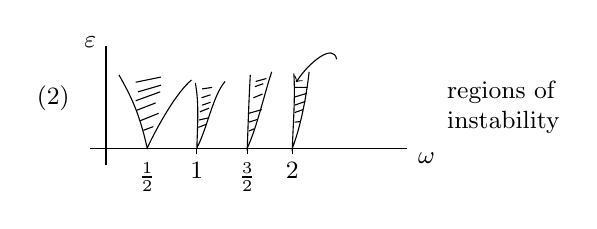
\begin{tikzpicture}[x=.97cm,y=.94cm,font=\small]
\draw (-.21,0)--(3.94,0);
\draw (0,-.23)--(0,1.38);
\node at (-.69,.67) {(2)};
\node[left] at (0,1.43) {$\varepsilon$};
\node[right] at (3.96,-.13) {$\omega$};
\draw (.17,.99) .. controls (.31,.73) and (.43,.51) .. (.54,0)
 .. controls (.68,.31) and (.93,.76) .. (1.12,.92);
\draw (.49,.24)--(.62,.29) (.45,.37)--(.69,.47)
 (.4,.51)--(.65,.61) (.39,.64)--(.71,.76)
 (.42,.76)--(.72,.85) (.39,.89)--(.72,.96);
\draw (1.17,.88) .. controls (1.22,.61) and (1.2,.33) .. (1.19,0)
 .. controls (1.33,.28) and (1.4,.71) .. (1.56,.9);
\draw (1.21,.28)--(1.31,.32) (1.22,.38)--(1.35,.41)
 (1.23,.49)--(1.35,.54) (1.26,.58)--(1.37,.62)
 (1.25,.68)--(1.37,.72) (1.26,.8)--(1.39,.82);
\draw (1.89,.99) .. controls (1.87,.63) and (1.86,.27) .. (1.85,0)
 .. controls (1.98,.29) and (2.07,.72) .. (2.17,1.03);
\draw (1.87,.23)--(1.94,.26) (1.87,.35)--(1.99,.39)
 (1.87,.47)--(2.04,.52) (1.93,.68)--(2.05,.73)
 (1.95,.83)--(2.06,.87) (1.96,.9)--(2.1,.94);
\draw (2.46,1.01) .. controls (2.48,.68) and (2.45,.31) .. (2.44,0)
 .. controls (2.54,.26) and (2.62,.66) .. (2.66,1.03);
\draw (2.47,.35)--(2.55,.36) (2.47,.48)--(2.58,.52)
 (2.47,.58)--(2.61,.63) (2.47,.69)--(2.63,.74)
 (2.47,.82)--(2.64,.82);
\draw[->] (3.02,1.2) .. controls (2.98,1.43) and (2.65,1.15) .. (2.49,.89);
\draw (1.19,0)--(1.19,-.08) (1.85,0)--(1.85,-.08) (2.44,0)--(2.44,-.08);
\node[below] at (.54,-.06) {$\frac12$};
\node[below] at (1.19,-.06) {$1$};
\node[below] at (1.85,-.06) {$\frac32$};
\node[below] at (2.44,-.06) {$2$};
\node[align=left,anchor=west] at (4.34,.55) {regions of\\instability};
\end{tikzpicture}}\endgroup
\end{center}
}
\end{GelfandAdjacentEvidence}
\begin{GelfandAdjacentEvidence}{GELFAND-P001081}{3}


$a(t)=\cos t\quad\Rightarrow$ increasingly high order of contact (of the zone boundaries).
\SourceFigure{GELFAND-P001081}{mathieu-tongue}{%
\begin{center}
\begingroup\color{black}\GelfandFitDiagram{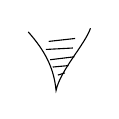
\begin{tikzpicture}[x=.93cm,y=.93cm]
\draw (-.38,.8) .. controls (-.16,.55) and (-.03,.32) .. (0,0)
 .. controls (.06,.28) and (.39,.62) .. (.47,.85);
\draw (.025,.21)--(.12,.24) (-.045,.32)--(.17,.34)
 (-.08,.42)--(.25,.46) (-.14,.56)--(.23,.58) (-.1,.67)--(.26,.71);
\end{tikzpicture}}\endgroup
\end{center}
Sketch above the words “zone boundaries.”}
\end{GelfandAdjacentEvidence}
\begin{GelfandAdjacentEvidence}{GELFAND-P001081}{4}


(3) \uline{Theorem.} Width of the $N$th zone $\asymp\varepsilon^{[\frac Np]}$;
if $a$ is a trigonometric polynomial
\[
\deg a=p.
\]
\Unclear{GELFAND-P001081}{zone-width-exponent}{The exponent is written $[N/p]$. The brackets are left unexplained.}
\end{GelfandAdjacentEvidence}
\begin{GelfandAdjacentEvidence}{GELFAND-P001081}{5}


\dashuline{Mathieu}: $p=1$.
\Unclear{GELFAND-P001081}{mathieu-name}{The handwritten name appears to read «Мате».}
\end{GelfandAdjacentEvidence}
\begin{GelfandAdjacentEvidence}{GELFAND-P001081}{6}


Hill’s equation ($a$ in general position) $\Rightarrow$ first-order contact everywhere
\SourceFigure{GELFAND-P001081}{hill-tongue}{%
\begin{center}
\begingroup\color{black}\GelfandFitDiagram{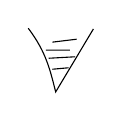
\begin{tikzpicture}[x=.93cm,y=.93cm]
\draw (-.42,.87) .. controls (-.17,.54) and (-.12,.29) .. (-.045,0)--(.47,.86);
\draw (-.09,.31)--(.13,.33) (-.14,.46)--(.22,.48)
 (-.18,.57)--(.15,.57) (-.09,.68)--(.24,.72);
\end{tikzpicture}}\endgroup
\end{center}
Sketch after the arrow.}
\end{GelfandAdjacentEvidence}
\begin{GelfandAdjacentEvidence}{GELFAND-P001081}{7}


(but the width decreases exponentially)

\dashuline{Question by I. M. G.}: \dashuline{$\omega^2$ — a $0$-zone potential}.
What happens near a $1$-zone potential?
\SourceFigure{GELFAND-P001081}{gelfand-question}{The question about a one-zone potential.}
\end{GelfandAdjacentEvidence}
\begin{GelfandAdjacentEvidence}{GELFAND-P001081}{8}


\dashuline{The proof} depends on the structure of the Rayleigh–Schrödinger series. We seek the perturbation.
\begin{equation*}
(4)\quad
(\Lambda+\varepsilon A)(\xi_0+\varepsilon\xi_1+\ldots)
=(\xi_0+\varepsilon\xi_1+\ldots)(\lambda_0+\varepsilon\lambda_1+\ldots)
\end{equation*}
\SourceFigure{GELFAND-P001081}{perturbation-series}{The perturbation series in equation (4).}
\end{GelfandAdjacentEvidence}



\Needspace{7\baselineskip}
\begin{GelfandAdjacentEvidence}{GELFAND-P001082}{1}
\SourcePage{GELFAND-P001082}{unlabelled}
series are [combined?] and depend on the numbers named for \uline{Catalan}:
\Unclear{GELFAND-P001082}{first-line-abbreviation}{The abbreviation appears to read «сверт.».}
\end{GelfandAdjacentEvidence}
\begin{GelfandAdjacentEvidence}{GELFAND-P001082}{2}

\[
1\quad 1\quad 2\quad 5\quad 14\quad 42\quad 138
\]
\SourceFigure{GELFAND-P001082}{catalan-number}{The last number in the manuscript is $138$.}
\end{GelfandAdjacentEvidence}
\begin{GelfandAdjacentEvidence}{GELFAND-P001082}{3}


Another occurrence, in Griffiths and Harris (they did not notice).

\uline{Formula}:
\[
(5)\qquad a_{n+1}=\sum_{j=1}^{n-1}a_j a_{n-j}
\]
\SourceFigure{GELFAND-P001082}{catalan-recurrence}{The summation bounds and indices in the manuscript.}
\end{GelfandAdjacentEvidence}
\begin{GelfandAdjacentEvidence}{GELFAND-P001082}{4}


Using a generating function we compute
\[
a_n=\frac{(2n)!}{n!(n+1)!}
\]
($=$ the number of simplicial subdivisions of an $n$-gon)
\SourceFigure{GELFAND-P001082}{polygon-index}{The polygon index in the manuscript.}
\end{GelfandAdjacentEvidence}
\begin{GelfandAdjacentEvidence}{GELFAND-P001082}{5}


[Inserted at the upper left, “Griffiths, Harris”:]\\
Riemann surfaces of genus $g$ have $3g-3$ moduli.
\SourceFigure{GELFAND-P001082}{griffiths-harris-insertion}{The names inserted above the line.}
\end{GelfandAdjacentEvidence}
\begin{GelfandAdjacentEvidence}{GELFAND-P001082}{6}


On $S^2=\mathbb C P^1$ choose branch points, etc.

GH: the number of ways in which one [crossed out] and the same surface was obtained:
\Unclear{GELFAND-P001082}{genus-cancel}{The crossed-out word may be an abbreviation for “surface.”}
\end{GelfandAdjacentEvidence}
\begin{GelfandAdjacentEvidence}{GELFAND-P001082}{7}

\[
1,1,2,5,\ldots\quad\text{— Catalan numbers (but it is not said why)}
\]

\dashuline{Bracket symbol}: an expression properly formed from letters and brackets:
example
\[
((a))b\,(cd)e
\]
\[
\sum\text{of the counts of symbols and opening brackets}=n\quad\text{(length)}
\]
\[
\Downarrow
\]
count $=$ the Catalan number

\SourceFigure{GELFAND-P001082}{bracket-symbol-examples}{%
\begin{center}
\begingroup\color{black}\GelfandFitDiagram{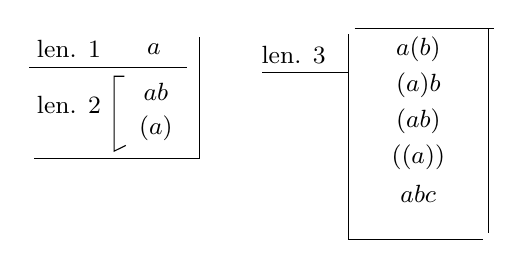
\begin{tikzpicture}[x=.87cm,y=.61cm,font=\small]
\node at (.45,0) {len. 1};
\node at (1.69,0) {$a$};
\draw (-.13,-.38)--(2.18,-.38);
\draw (2.35,.25)--(2.35,-2.28)--(-.06,-2.28);
\node at (.45,-1.15) {len. 2};
\node at (1.72,-.88) {$ab$};
\node at (1.72,-1.65) {$(a)$};
\draw (1.26,-.56)--(1.11,-.56)--(1.11,-2.12)--(1.28,-2.0);
\node at (3.73,-.12) {len. 3};
\draw (3.27,-.48)--(4.53,-.48);
\draw (4.53,.31)--(4.53,-3.95)--(6.49,-3.95);
\draw (4.62,.43)--(6.65,.43) (6.58,.43)--(6.58,-3.83);
\node at (5.55,.0) {$a(b)$};
\node at (5.55,-.75) {$(a)b$};
\node at (5.55,-1.5) {$(ab)$};
\node at (5.55,-2.25) {$((a))$};
\node at (5.55,-3) {$abc$};
\end{tikzpicture}}\endgroup
\end{center}
}
\end{GelfandAdjacentEvidence}
\begin{GelfandAdjacentEvidence}{GELFAND-P001082}{8}


Bracket symbol $\rightsquigarrow$ term of the perturbation series.
\[
\underset{\text{eigenvalues}}{\lambda_i}\quad\rightsquigarrow\quad\text{quiver}
\]

\uwave{Eigenvalues.}\qquad $\Lambda$ — diagonal operator,
\qquad $\Lambda_i:V_i\longrightarrow V_i$

\SourceFigure{GELFAND-P001082}{diagonal-operator-diagram}{%
\begin{center}
\begingroup\color{black}\GelfandFitDiagram{\begin{tikzpicture}[x=.85cm,y=.85cm,font=\small]
\node at (-.56,-.78) {(6)};
\draw (0,-2.15)--(0,.2)--(2.55,.2);
\draw (0,-.36)--(.56,-.36)--(.56,.2);
\node at (.28,-.07) {$\Lambda_i$};
\draw (.56,-.36) rectangle (1.06,-.86);
\draw[dotted,thick] (1.18,-.99)--(2.38,-2.14);
\end{tikzpicture}}\endgroup
\end{center}
\[
\underset{\text{matrix element of the perturbation}}{A_{i,j}:V_i\longrightarrow V_j}
\]
}
\end{GelfandAdjacentEvidence}
\begin{GelfandAdjacentEvidence}{GELFAND-P001082}{9}


\SourceFigure{GELFAND-P001082}{quiver-diagram}{%
\begin{center}
\begingroup\color{black}\GelfandFitDiagram{\begin{tikzpicture}[x=.97cm,y=.94cm,font=\small]
\node[anchor=west] at (-.65,.72) {Quiver.};
\coordinate (i) at (0,0);
\coordinate (j) at (1.6,0);
\fill (i) circle (1.7pt) (j) circle (1.7pt);
\draw[->] (i) .. controls (.4,.18) and (.84,.22) .. (1.08,.13);
\draw (1.08,.13) .. controls (1.3,.1) and (1.49,.04) .. (j);
\draw[->] (1.49,-.12) .. controls (1.24,-.26) and (.81,-.3) .. (.52,-.23);
\draw (.52,-.23) .. controls (.33,-.15) and (.14,-.14) .. (.07,-.14);
\draw[->] (-.04,.23) .. controls (-.24,.81) and (-.81,.43) .. (-.79,-.06)
 .. controls (-.76,-.54) and (-.37,-.35) .. (-.17,-.23);
\node at (-.02,-.45) {$i$};
\node at (1.55,-.54) {$j$};
\node at (3.08,.46) {\uwave{to an arrow $\rightsquigarrow A_{i,j}$}};
\node at (-.02,-1.05) {$V_i$};
\node at (1.55,-1.15) {$V_j$};
\node[align=left,anchor=west] at (1.9,-1.08) {— eigenspaces\\(vertices)};
\end{tikzpicture}}\endgroup
\end{center}
}
\end{GelfandAdjacentEvidence}



\Needspace{7\baselineskip}
\begin{GelfandAdjacentEvidence}{GELFAND-P001083}{1}
\SourcePage{GELFAND-P001083}{9}
Suppose everything is finite or locally finite

(into $\forall$ vertex there lead finitely many)

Mathieu’s equation — the quiver is incomplete!
\Unclear{GELFAND-P001083}{mathieu-name-top}{The handwritten name appears to read «Мате».}
\end{GelfandAdjacentEvidence}
\begin{GelfandAdjacentEvidence}{GELFAND-P001083}{2}


(locally finite)

(the potential — $\cos$ and $\sin$ and the eigenfunctions too!)

\uline{Mathieu} (with a trigonometric polynomial) $\Rightarrow$ a matrix of generalized Jacobi type.
\Unclear{GELFAND-P001083}{mathieu-name-lower}{The handwritten name appears to read «Мате».}
\end{GelfandAdjacentEvidence}
\begin{GelfandAdjacentEvidence}{GELFAND-P001083}{3}


We seek the perturbation of $\lambda_0$.

\SourceFigure{GELFAND-P001083}{spectral-graph-diagram}{%
\begin{center}
\begingroup\color{black}\GelfandFitDiagram{\begin{tikzpicture}[x=1.04cm,y=1.04cm]
\draw (-.47,0)--(2.1,0);
\draw (0,0)--(0,1.41);
\draw (-.48,-.17)--(2.18,.45);
\node[left] at (0,1.33) {$\displaystyle\bigoplus_{i\ne0}V_i$};
\node[below] at (2.16,0) {$V_0$};
\node[below] at (.9,-.06) {$\lambda_0$};
\node[right] at (2.18,.45) {$V_0(\varepsilon)$};
\end{tikzpicture}}\endgroup
\end{center}
}
\end{GelfandAdjacentEvidence}
\begin{GelfandAdjacentEvidence}{GELFAND-P001083}{4}


$V_0(\varepsilon)$ — a subspace, [below: “eigen”] depending analytically on
$\varepsilon$, corresponding to eigenvectors close to $\lambda_0$.
\SourceFigure{GELFAND-P001083}{eigenvalue-word}{The manuscript abbreviation for “eigenvectors.”}
\end{GelfandAdjacentEvidence}
\begin{GelfandAdjacentEvidence}{GELFAND-P001083}{5}


\[
(7)\quad
(\Lambda+\varepsilon A)(E_0+B(\varepsilon))
=(E_0+B(\varepsilon))(\lambda_0+\varepsilon\alpha^1+\ldots)
\]
\SourceFigure{GELFAND-P001083}{coefficient-symbol}{The coefficient $\alpha^1$ in formula (7).}
\end{GelfandAdjacentEvidence}
\begin{GelfandAdjacentEvidence}{GELFAND-P001083}{6}


$V_0(\varepsilon)$ — the graph of the operator
\[
B(\varepsilon):V_0\longrightarrow\bigoplus_{i\ne0}V_i
\qquad E_0\text{ — the projector onto }V_0
\]
\[
\alpha^1:\text{ operator }V_0\to V_0,\qquad \alpha^i:V_0\to V_0
\]

(7) — the condition of invariance of [crossed out] $V_0(\varepsilon)$
\Unclear{GELFAND-P001083}{invariance-cancel}{The crossed-out symbol is illegible.}
\end{GelfandAdjacentEvidence}
\begin{GelfandAdjacentEvidence}{GELFAND-P001083}{7}


(8) operator $\lambda_0+\varepsilon\alpha^1+\ldots$ is called
\uwave{the secular} operator (in physics)
\Unclear{GELFAND-P001083}{secular-ending}{A correction is visible above the ending of the Russian word for “secular.” The original ending is uncertain.}
\end{GelfandAdjacentEvidence}
\begin{GelfandAdjacentEvidence}{GELFAND-P001083}{8}


The restriction of $\Lambda+\varepsilon A$ to $V_0(\varepsilon)$
is similar to the secular operator (8) $\Rightarrow$ they have the same eigenvalues.

\uwave{Formula for $\alpha^k$}:
\[
(9)\qquad \alpha_k=\sum_{\gamma:\lvert\gamma\rvert=k}
\bigl(\Pi_\gamma(A)Q_\gamma(\Lambda)\bigr)
\]
\SourceFigure{GELFAND-P001083}{loop-coefficient-formula}{The heading uses a superscript and formula (9) a subscript.}
\end{GelfandAdjacentEvidence}
\begin{GelfandAdjacentEvidence}{GELFAND-P001083}{9}


$\gamma$ — a loop in the quiver from $0$ to $0$

$k$ — the length of the loop

\SourceFigure{GELFAND-P001083}{loop-diagram}{%
\begin{center}
\begingroup\color{black}\GelfandFitDiagram{\begin{tikzpicture}[x=1.06cm,y=1.06cm]
\coordinate (origin) at (0,1.46);
\coordinate (first) at (1.96,1.66);
\coordinate (left) at (.34,-.07);
\coordinate (right) at (1.25,-.02);
\coordinate (m) at (-1.39,.02);
\node at (-1.78,.99) {(10)};
\node[above left] at (origin) {$0$};
\node[right] at (first) {$i$};
\node[below left] at (m) {$m$};
\node[below right] at (left) {$j$};
\node[right] at (right) {$j$};
\node at (1.03,.99) {$\gamma$};
\draw[->] (m)--(-.43,1.02);
\draw (-.43,1.02)--([xshift=-.07cm,yshift=-.06cm]origin);
\draw[->] ([xshift=.11cm]origin)--(1.25,1.58);
\draw (1.25,1.58)--(first);
\draw[->] (first)--(1.62,.82);
\draw (1.62,.82)--(right);
\draw[->] ([xshift=-.15cm]right)--(.26,1.12);
\draw (.26,1.12)--(origin);
\draw[->] (origin)--(.26,.44);
\draw (.26,.44)--(left);
\draw[->] ([xshift=-.03cm]left)--(-.97,.015);
\draw (-.97,.015)--(m);
\draw[<->] (.73,-.26)--(1.22,-.19);
\draw[->] (.61,-.17)--(.36,.06);
\end{tikzpicture}}\endgroup
\end{center}
Both lower labels look like $j$. The connection of the short diagonal stroke to the adjacent arrows is uncertain.}
\end{GelfandAdjacentEvidence}
\begin{GelfandAdjacentEvidence}{GELFAND-P001083}{10}


\[
\Pi_\gamma(A)=A_{m0}\ldots A_{ij}A_{0i}
\]

$\Pi_\gamma(A)$ — the chronological product around the loop
($=\prod A_{i,j}$ in the required order along the loop)
[inserted below: «following the arrows».]
\SourceFigure{GELFAND-P001083}{chronological-insertion}{The insertion below the note about the order of factors.}
\end{GelfandAdjacentEvidence}


$Q_\gamma(\Lambda)$ — a rational function of the eigenvalues

(computed using Catalan numbers!)

Consider a bracket symbol.

\uwave{Filling it} — insert vertices of the quiver in place of the letters.


\Needspace{7\baselineskip}
\begin{GelfandAdjacentEvidence}{GELFAND-P001084}{1}
\SourcePage{GELFAND-P001084}{unlabelled}
A loop is constructed from a filling.

\Unclear{GELFAND-P001084}{top-cancel}{The crossed-out mark before “terms” is illegible.}
\end{GelfandAdjacentEvidence}
\begin{GelfandAdjacentEvidence}{GELFAND-P001084}{2}

The terms must be indexed by fillings

\[
\Vert\quad 0\longrightarrow 0\longrightarrow i\longrightarrow j\longrightarrow 0
\]
\SourceFigure{GELFAND-P001084}{first-loop}{The chain of four arrows with two initial zeros.}
\end{GelfandAdjacentEvidence}
\begin{GelfandAdjacentEvidence}{GELFAND-P001084}{3}


\[
\begin{array}{cl}
(i)j & \\
\downarrow & \\
0 & \text{for an opening bracket, we omit the closing ones}
\end{array}
\]
\SourceFigure{GELFAND-P001084}{bracket-rule}{The arrow from the opening bracket to zero and its explanation.}
\end{GelfandAdjacentEvidence}
\begin{GelfandAdjacentEvidence}{GELFAND-P001084}{4}


There is one more arrow than the length of the filling.

One loop comes from different fillings.

\[
0\longrightarrow i\longrightarrow j\longrightarrow 0
\longrightarrow j\longrightarrow m\longrightarrow 0
\]
\SourceFigure{GELFAND-P001084}{second-loop}{The loop with two occurrences of vertex $j$.}
\end{GelfandAdjacentEvidence}
\begin{GelfandAdjacentEvidence}{GELFAND-P001084}{5}


In fact, the sum runs over fillings rather than loops.

[Line crossed out: $ij(jm)\quad ij(jm)$ not unamb…]
\Unclear{GELFAND-P001084}{cancelled-fillings}{Two similar fillings are legible in the crossed-out line. At the right, possibly “not unamb…”.}
\end{GelfandAdjacentEvidence}
\begin{GelfandAdjacentEvidence}{GELFAND-P001084}{6}


$ij(jm\qquad$ ambiguous closing bracket!! —
\SourceFigure{GELFAND-P001084}{closing-bracket-ambiguity}{The expression with the closing bracket omitted and its accompanying remark.}
\end{GelfandAdjacentEvidence}
\begin{GelfandAdjacentEvidence}{GELFAND-P001084}{7}


\tikz[baseline=(repeat.base)]{\node[draw,rounded corners=3pt,inner sep=2pt] (repeat) {repeat};}\quad [crossed out] contribution [crossed out]
\Unclear{GELFAND-P001084}{cancelled-before-exit}{Below the circled word, the crossed-out text probably reads “— the same.”}
\end{GelfandAdjacentEvidence}
\begin{GelfandAdjacentEvidence}{GELFAND-P001084}{8}

\Unclear{GELFAND-P001084}{cancelled-after-exit}{After “contribution,” the crossed-out text probably reads “different brackets!!”.}
\end{GelfandAdjacentEvidence}
\begin{GelfandAdjacentEvidence}{GELFAND-P001084}{9}


Diagram of a filling: add dashed [\sout{brackets}] [inserted below: arrows]
\Unclear{GELFAND-P001084}{overwritten-adjective-ending}{The ending of the Russian word for “dashed” is overwritten. The original ending is uncertain.}
\end{GelfandAdjacentEvidence}
\begin{GelfandAdjacentEvidence}{GELFAND-P001084}{10}


\SourceFigure{GELFAND-P001084}{filling-diagram}{%
\begin{center}
\begingroup\color{black}\GelfandFitDiagram{\begin{tikzpicture}[x=1cm,y=.86cm,font=\small]
\node at (-1.12,-.04) {$(i)j$};
\node (outerleft) at (0,0) {$0$};
\node (opening) at (1.04,.01) {$0$};
\node (inside) at (2.19,.05) {$i$};
\node (outside) at (3.27,.09) {$j$};
\node (outerright) at (4.5,.13) {$0$};
\draw[->] (outerleft)--(opening);
\draw[->] (opening)--(inside);
\draw[->] (inside)--(outside);
\draw[->] (outside)--(outerright);
\draw[->,dashed] (inside.north) to[bend right=53] (opening.north);
\draw (.1,-.39)--(.1,-.81)--(-.44,-.78);
\draw (4.44,-.22)--(4.44,-.48)--(5.13,-.48);
\end{tikzpicture}}\endgroup
\end{center}
}
\end{GelfandAdjacentEvidence}
\begin{GelfandAdjacentEvidence}{GELFAND-P001084}{11}

The outermost zeros do not signify anything

Arrow $\longrightarrow$ to $0$, that corresponds to the opening bracket matching
[crossed out] the closing bracket (from the letter before the closing bracket)
\Unclear{GELFAND-P001084}{cancelled-open}{The crossed-out word probably abbreviates “opening.”}
\end{GelfandAdjacentEvidence}
\begin{GelfandAdjacentEvidence}{GELFAND-P001084}{12}


\begin{equation*}
\alpha_k=\sum_{I,\ \lvert I\rvert=k-1}\frac{\Pi_{\gamma(I)}(A)}{q_I(\Lambda)}
\tag{11}
\end{equation*}
\SourceFigure{GELFAND-P001084}{coefficient-formula}{The left side of formula (11) reads $\alpha_k$.}
\end{GelfandAdjacentEvidence}
\begin{GelfandAdjacentEvidence}{GELFAND-P001084}{13}


\[
\begin{array}{l}
I\\[-.3ex]
\vert\\[-.3ex]
\text{filling of a bracket symbol}
\end{array}
\qquad
\lvert I\rvert\text{ — length of the bracket symbol}
\]
\SourceFigure{GELFAND-P001084}{bracket-symbol-ending}{The two annotations for the summation index.}
\end{GelfandAdjacentEvidence}
\begin{GelfandAdjacentEvidence}{GELFAND-P001084}{14}


$\Pi_{\gamma(I)}(A)$ — the chronological product around the loop along the solid arrows.

\begin{equation*}
q_I(\Lambda)=
\underset{\substack{\text{solid}\\\text{arrows}\\\text{into }i}}
{\prod_{i\ne0}}(\lambda_0-\lambda_i)
\underset{\substack{\text{dashed}\\\text{arrows}\\\text{from }j}}
{\prod_{j\ne0}}(\lambda_j-\lambda_0)
\tag{12}
\end{equation*}
\SourceFigure{GELFAND-P001084}{denominator-formula}{The factors and annotations for the two products in formula (12).}
\end{GelfandAdjacentEvidence}
\begin{GelfandAdjacentEvidence}{GELFAND-P001084}{15}


\[
(i)j\rightsquigarrow
(\lambda_0-\lambda_i)(\lambda_0-\lambda_j)(\lambda_i-\lambda_0)
\]
\SourceFigure{GELFAND-P001084}{denominator-example}{The product for the filling $(i)j$.}
\end{GelfandAdjacentEvidence}



\Needspace{7\baselineskip}
\begin{GelfandAdjacentEvidence}{GELFAND-P001085}{1}
\SourcePage{GELFAND-P001085}{10}
For even trigonometric polynomials, formula (9) suffices

[Below the word “even”: (for $\cos$)]

(and separately for $\sin$ as well)
\SourceFigure{GELFAND-P001085}{cosine-insertion}{The cosine annotation below the word “even.”}
\end{GelfandAdjacentEvidence}
\begin{GelfandAdjacentEvidence}{GELFAND-P001085}{2}


\[
V=\bigoplus V_i
\]
\begin{equation*}
\Lambda=\frac{d^2}{dt^2},\qquad
V_k=\{e_k,e_{-k}\},\qquad e_k=e^{ikt}
\tag{13}
\end{equation*}
\SourceFigure{GELFAND-P001085}{fourier-basis}{The notation for the operator and basis in equation (13).}
\end{GelfandAdjacentEvidence}
\begin{GelfandAdjacentEvidence}{GELFAND-P001085}{3}


\[
\begin{array}{c c c c c c c}
 & V_0, & V_1, & V_2 & V_3 & \cdots & V_k\\
\dim & 1 & 2 & 2 & 2 & & 2\\
 & & & & & & \lambda=-k^2
\end{array}
\]
\SourceFigure{GELFAND-P001085}{eigenspace-dimensions}{The dimensions and the eigenvalue in the last column.}
\end{GelfandAdjacentEvidence}
\begin{GelfandAdjacentEvidence}{GELFAND-P001085}{4}


$A$ — multiplication by a trigonometric polynomial

\begin{equation*}
a(t)=\sum_{\lvert s\rvert\le p}a_se_s
\tag{14}
\end{equation*}

Let it be even, i.e.
\begin{equation*}
a_{-s}=a_s
\tag{15}
\end{equation*}

\begin{equation*}
A_{i,j}=
\begin{pmatrix}
a_{j-i} & a_{i+j}\\
a_{-i-j} & a_{i-j}
\end{pmatrix}
\qquad (?)
\tag{16}
\end{equation*}
\SourceFigure{GELFAND-P001085}{matrix-display}{The signs in the subscripts and the question mark beside equation (16).}
\end{GelfandAdjacentEvidence}
\begin{GelfandAdjacentEvidence}{GELFAND-P001085}{5}


$(16)\Rightarrow$ if $i+j>p$, the matrices are diagonal and even \uline{scalar}
[written below: (by (15))] in this basis.

If all $A_{i,j}$ in the loop are scalar, then the product is also scalar.

\begin{equation*}
\underline{\tau p<2k}\quad\Rightarrow\quad
\text{\uwave{$\alpha_\tau$ is scalar}}
\tag{17}
\end{equation*}
\SourceFigure{GELFAND-P001085}{scalar-lemma}{The coefficient $\alpha_\tau$ and the underlining in equation (17).}
\end{GelfandAdjacentEvidence}
\begin{GelfandAdjacentEvidence}{GELFAND-P001085}{6}


This is a topological lemma (from combinatorial topology).

\uline{Proof}

\SourceFigure{GELFAND-P001085}{proof-number-line}{%
\begin{center}
\begingroup\color{black}\GelfandFitDiagram{\begin{tikzpicture}[x=.59cm,y=.72cm,font=\small]
\draw (-.88,0)--(0,0)--(1.31,.06)--(3.38,.02)--(6.05,-.09)--(9.23,-.16);
\foreach \x/\y in {0/0,.62/.02,1.31/.06,1.96/.045,2.70/.034,3.38/.02,
  4.15/-.01,4.80/-.04,5.34/-.06,6.05/-.09,6.79/-.105,7.43/-.12,
  8.12/-.135,8.74/-.15}
  \draw (\x,\y-.13)--(\x,\y+.13);
\node at (0,-.44) {$-k$};
\node at (4.15,-.45) {$0$};
\node at (8.74,-.56) {$k$};
\end{tikzpicture}}\endgroup
\end{center}
}
\end{GelfandAdjacentEvidence}
\begin{GelfandAdjacentEvidence}{GELFAND-P001085}{7}


Consider a loop of $\tau$ arrows of length $\le p$.

Then for $\forall$ arrow $i+j>p$

(homotopic to $0$!)

$i+j\le p\ \Rightarrow$ a jump across
\Unclear{GELFAND-P001085}{crossing-word}{Provisional reading “a jump across.”}
\end{GelfandAdjacentEvidence}
\begin{GelfandAdjacentEvidence}{GELFAND-P001085}{8}


\SourceFigure{GELFAND-P001085}{loop-arches}{%
\begin{center}
\begingroup\color{black}\GelfandFitDiagram{\begin{tikzpicture}[x=1.16cm,y=.83cm,font=\small]
\draw (-1.8,.16) .. controls (-1.32,.54) and (-.84,.87) .. (-.34,.49)
 .. controls (-.21,.41) and (-.11,.33) .. (-.11,.12)
 .. controls (-.01,.37) and (.33,.37) .. (.46,.11)
 .. controls (.59,.42) and (1.56,.98) .. (2.13,.23);
\node[below] at (-1.84,.07) {$-k$};
\node[below] at (2.18,.05) {$+k$};
\node at (2.24,.03) {$i$};
\end{tikzpicture}}\endgroup
\end{center}
The small mark at the right end looks like $i$. Arrowheads on the arches are indistinct.}
\end{GelfandAdjacentEvidence}

$\Rightarrow$ length $\le\tau p$ and so on.

$(17)\Rightarrow$ in this approximation the eigenvalue has yet to split $\Rightarrow$

$\Rightarrow$ the required inequality!


\Needspace{7\baselineskip}
\begin{GelfandAdjacentEvidence}{GELFAND-P001086}{1}
\SourcePage{GELFAND-P001086}{unlabelled}
An involution is also used:
\[
(((a))b)(cd)e
\]
\SourceFigure{GELFAND-P001086}{original-bracket-symbol}{The original bracket symbol.}
\end{GelfandAdjacentEvidence}
\begin{GelfandAdjacentEvidence}{GELFAND-P001086}{2}


use the opening brackets to divide it into fragments
\[
a))b)\qquad cd)e
\]
\SourceFigure{GELFAND-P001086}{first-fragments}{The fragments with their opening brackets removed.}
\end{GelfandAdjacentEvidence}
\begin{GelfandAdjacentEvidence}{GELFAND-P001086}{3}


Attach the closing brackets to the letter. Rearrange the letters in the fragments
[inserted below at the left: in reverse order]
\SourceFigure{GELFAND-P001086}{reverse-order-insertion}{The insertion specifying the reverse order of the letters.}
\end{GelfandAdjacentEvidence}
\begin{GelfandAdjacentEvidence}{GELFAND-P001086}{4}

\[
b)a))\qquad ed)c
\]
\SourceFigure{GELFAND-P001086}{reversed-fragments}{The two fragments with their letters in reverse order.}
\end{GelfandAdjacentEvidence}
\begin{GelfandAdjacentEvidence}{GELFAND-P001086}{5}


[crossed out] Put the opening brackets back in their former places
\Unclear{GELFAND-P001086}{cancel-before-stavim}{The crossed-out abbreviation before “Put” is illegible.}
\end{GelfandAdjacentEvidence}
\begin{GelfandAdjacentEvidence}{GELFAND-P001086}{6}

\[
(((b)a))(ed)c
\]
\SourceFigure{GELFAND-P001086}{dual-bracket-symbol}{The dual bracket symbol.}
\end{GelfandAdjacentEvidence}
\begin{GelfandAdjacentEvidence}{GELFAND-P001086}{7}


\uwave{We obtain the dual symbol}

Its contribution is obtained by swapping the diagonal entries.
\SourceFigure{GELFAND-P001086}{final-abbreviation}{The Russian word for “diagonal” is abbreviated at the end of the line.}
\end{GelfandAdjacentEvidence}



\Needspace{7\baselineskip}
\begin{GelfandAdjacentEvidence}{GELFAND-P001087}{1}
\SourcePage{GELFAND-P001087}{unlabelled}
\uline{28/II-83}\qquad\uuline{Gelfand Seminar}.

\uline{I. Krichever.}
\SourceFigure{GELFAND-P001087}{krichever-heading}{The date, seminar name, and speaker.}
\end{GelfandAdjacentEvidence}
\begin{GelfandAdjacentEvidence}{GELFAND-P001087}{2}


The aim is to construct a formal perturbation theory for the perturbation of the KdV equation.
\begin{equation*}
(1)\qquad
u_t-\frac{\partial}{\partial x}
\underset{\frac{\delta I_3}{\delta u}}{%
\tikz[baseline=(term.base)]{
\node[inner sep=1pt] (term) {$\displaystyle\left(\frac14u_{xx}-\frac34u^2\right)$};
\draw (term.south west) -- ++(0,-.8mm) -| (term.south east);
}}
=\varepsilon K[u]
\end{equation*}
[Below $K$: differential polynomial in $u$.]
\SourceFigure{GELFAND-P001087}{perturbed-kdv-equation}{Equation (1) with a square-ended bracket and the annotation below $K$.}
\end{GelfandAdjacentEvidence}
\begin{GelfandAdjacentEvidence}{GELFAND-P001087}{3}


[Crossed out: \sout{\(u=u_0\)}.]
\SourceFigure{GELFAND-P001087}{cancelled-initial-condition}{The crossed-out equality before (2).}
\end{GelfandAdjacentEvidence}
\begin{GelfandAdjacentEvidence}{GELFAND-P001087}{4}

\[
(2)\qquad u=u_0(x,t)+\varepsilon(\ldots)
\]
KdV
\begin{equation*}
(3)\qquad
u_t-\frac{\partial}{\partial x}
\underset{\substack{\Vert\\[.1ex]\frac{\delta I_3}{\delta u}}}{%
\tikz[baseline=(term.base)]{
\node[inner sep=1pt] (term) {$\displaystyle\left(\frac14u_{xx}-\frac34u^2\right)$};
\draw (term.south west) -- ++(0,-.8mm) -| (term.south east);
}}
=0,\qquad I_3=\frac14(u_x^2+u^3).
\end{equation*}
\Unclear{GELFAND-P001087}{eq03-variational-annotation}{Two short vertical strokes stand between the lower bracket and its label. Their meaning is uncertain.}
\end{GelfandAdjacentEvidence}
\begin{GelfandAdjacentEvidence}{GELFAND-P001087}{5}


There is an infinite series of integrals in involution $I_k$: $I_1=u$, $I_2=u^2$, $\ldots$
\SourceFigure{GELFAND-P001087}{integrals-line}{The first integrals, including the overwritten $u$ in $I_1$.}
\end{GelfandAdjacentEvidence}
\begin{GelfandAdjacentEvidence}{GELFAND-P001087}{6}


A finite-gap solution is a solution that is a stationary point of the functional
\[
(4)\qquad H=I_{n+2}-\sum_{k=1}^{n+1}c_k I_k
\]
i.e. a solution of the equation
\[
(5)\qquad \frac{\delta H}{\delta u}=0
\]
\SourceFigure{GELFAND-P001087}{finite-gap-stationary}{The functional and its stationarity condition in equations (4) and (5).}
\end{GelfandAdjacentEvidence}
\begin{GelfandAdjacentEvidence}{GELFAND-P001087}{7}


Recurrence relation:
\[
(6)\qquad
\frac{d}{dx}\frac{\delta I_{n+1}}{\delta u}
=\left[\left(\frac{d}{dx}\right)^3+2u\frac{d}{dx}+u'\right]
\frac{\delta I_n}{\delta u}
\]
(up to coefficients).
\SourceFigure{GELFAND-P001087}{recursion-relation}{The coefficients, prime, and indices in equation (6).}
\end{GelfandAdjacentEvidence}
\begin{GelfandAdjacentEvidence}{GELFAND-P001087}{8}


\[
\delta^2 H\; -\; ?
\]
at a specified stationary point.
\SourceFigure{GELFAND-P001087}{second-variation}{The question about the second variation.}
\end{GelfandAdjacentEvidence}



\Needspace{7\baselineskip}
\begin{GelfandAdjacentEvidence}{GELFAND-P001088}{1}
\SourcePage{GELFAND-P001088}{15}
\[
L=-\frac{d^2}{dx^2}+u_0(x)\qquad
\text{spectrum:}\qquad (u_0(x+1)=u_0(x))
\]
\SourceFigure{GELFAND-P001088}{periodic-schrodinger-operator}{The operator and periodicity condition.}
\end{GelfandAdjacentEvidence}
\begin{GelfandAdjacentEvidence}{GELFAND-P001088}{2}


\SourceFigure{GELFAND-P001088}{spectrum-bands}{%
\begin{center}
\begingroup\color{black}\GelfandFitDiagram{\begin{tikzpicture}[x=.65cm,y=.64cm,font=\small]
\draw (0,0)--(.74,-.012) (1.39,.025)--(2.01,.003)
 (2.58,.003)--(3.36,.01) (3.76,.037)--(4.36,.063)
 (4.79,.026) to[out=5,in=177] (9.18,.095);
\foreach \x in {0,.74,1.39,2.01,2.58,3.36,3.76,4.36,4.79}
  \draw (\x,-.17)--(\x,.19);
\node[below] at (0,-.2) {$E_1$};
\node[below] at (.74,-.2) {$E_2$};
\node[below] at (1.39,-.2) {$E_3$};
\node[below] at (2.01,-.2) {$E_4$};
\node[below right] at (4.73,-.13) {$E_{2n+1}$};
\end{tikzpicture}}\endgroup
\end{center}
}
\end{GelfandAdjacentEvidence}
\begin{GelfandAdjacentEvidence}{GELFAND-P001088}{3}

The remaining endpoints are simple eigenvalues of the periodic and antiperiodic problems.

Quasimomentum differential:
\[
(7)\qquad
i\,dp=\frac{Q(E)dE}{\sqrt R}
=\frac{E^n+\sum_{k=1}^{n}r_kE^{n-k}}{\sqrt R}\,dE
\]
\Unclear{GELFAND-P001088}{eq07-polynomial-coefficient}{The coefficient is provisionally read as $r_k$. The first letter is ambiguous.}
\end{GelfandAdjacentEvidence}
\begin{GelfandAdjacentEvidence}{GELFAND-P001088}{4}

\[
R(E)=\prod_{i=1}^{2n+1}(E-E_i)
\]
[Crossed out at the right: \sout{(norm.}]
\Unclear{GELFAND-P001088}{cancel-normalized}{The beginning reads “(norm.”. The rest of the abbreviation is uncertain.}
\end{GelfandAdjacentEvidence}
\begin{GelfandAdjacentEvidence}{GELFAND-P001088}{5}


Conditions uniquely determining $dp$:
\[
\int_{E_{2i}}^{E_{2i+1}}dp=0
\]
(normalized Abelian differential of the second kind with its sole singularity at $\infty$ —\\
— a second-order pole.)
\SourceFigure{GELFAND-P001088}{quasimomentum-normalization}{The vanishing integral and the note on the pole.}
\end{GelfandAdjacentEvidence}
\begin{GelfandAdjacentEvidence}{GELFAND-P001088}{6}


Now consider the perturbation $u=u_0+\delta u$

$E_i'$ — new band edges

$e_s^-<e_s^+$ — new band edges; $\delta e_s=e_s^+-e_s^-$
\SourceFigure{GELFAND-P001088}{new-endpoints}{The two new edges and the definition of $\delta e_s$.}
\end{GelfandAdjacentEvidence}
\begin{GelfandAdjacentEvidence}{GELFAND-P001088}{7}


Then:
\[
(8)\qquad
\delta^2H=\frac12\sum Q(E_i)(\delta E_i)^2
+\frac14\sum_s Q(e_s)(\delta e_s)^2
\]
($e_s$ — double points of the spectrum)
\SourceFigure{GELFAND-P001088}{second-variation-equation}{The two sums of the second variation and the note on $e_s$.}
\end{GelfandAdjacentEvidence}
\begin{GelfandAdjacentEvidence}{GELFAND-P001088}{8}


$Q$ changes sign once in $\forall$ of the forbidden zones $\Rightarrow$ one zero in each zone
\SourceFigure{GELFAND-P001088}{zeros-of-q}{The handwritten phrase “one zero each.”}
\end{GelfandAdjacentEvidence}
\begin{GelfandAdjacentEvidence}{GELFAND-P001088}{9}


\SourceFigure{GELFAND-P001088}{q-sign-diagram}{%
\begin{center}
\begingroup\color{black}\GelfandFitDiagram{\begin{tikzpicture}[x=.63cm,y=.66cm,font=\small]
\node at (0,-.01) {$\ldots$};
\draw (1.37,0)--(1.93,0) (3.02,.03)--(3.76,.03);
\draw[->] (4.85,.035) to[out=2,in=176] (8.14,-.04);
\foreach \x in {1.37,1.93,3.02,3.76,4.85}
  \draw (\x,-.15)--(\x,.15);
\node at (1.67,.44) {$+$};
\node at (3.49,.52) {$-$};
\node at (6.04,.56) {$+$};
\node at (10.13,.17) {\uwave{sign of $Q$}};
\draw[->] (3.15,-.97)--(3.29,-.27);
\end{tikzpicture}}\endgroup
\end{center}
}
\end{GelfandAdjacentEvidence}
\begin{GelfandAdjacentEvidence}{GELFAND-P001088}{10}

[Below the arrow:] inside [crossed out] there may be other coalesced ones $\Rightarrow$ add another positive or negative square
\Unclear{GELFAND-P001088}{cancel-before-mogut}{The crossed-out word may read “will be.”}
\end{GelfandAdjacentEvidence}
\begin{GelfandAdjacentEvidence}{GELFAND-P001088}{11}

(from the second sum in (8))
\SourceFigure{GELFAND-P001088}{sign-caption}{The note below the arrow in the sign diagram.}
\end{GelfandAdjacentEvidence}
\begin{GelfandAdjacentEvidence}{GELFAND-P001088}{12}


\[
(9)\qquad L\Psi(x,E)=E\Psi
\]
\[
\Psi(x+1)=w\Psi,\qquad w=e^{iP},\qquad P=\int_{E_1}^{E}dp
\]
\SourceFigure{GELFAND-P001088}{bloch-equations}{The Bloch equation and multiplier.}
\end{GelfandAdjacentEvidence}
\begin{GelfandAdjacentEvidence}{GELFAND-P001088}{13}


Width of the opened gap
\[
(10)\qquad
(\delta e_s)^2=
\frac{\bigl|\langle(\delta u)\Psi^2\rangle\bigr|^2}{\langle|\Psi|^2\rangle}
\]
($\Psi$ — Bloch function, $\Psi(x,e_s)$)
\SourceFigure{GELFAND-P001088}{eq10-denominator}{The written denominator is $\langle\lvert \Psi\rvert^2\rangle$ with no outer exponent.}
\end{GelfandAdjacentEvidence}
\begin{GelfandAdjacentEvidence}{GELFAND-P001088}{14}


$\langle\qquad\rangle$ — averaging over a period

$u_0=\mathrm{const}\Rightarrow$ we obtain [crossed out: \sout{averag.} …] Fourier coefficients for the perturbation.
\Incomplete{GELFAND-P001088}{cancel-before-fourier}{After the start of “average,” one or more words are obscured by the cancellation strokes.}
\end{GelfandAdjacentEvidence}
\begin{GelfandAdjacentEvidence}{GELFAND-P001088}{15}


\uline{Problem (I. M. G.)}: compute the third variation, and so on.
\SourceFigure{GELFAND-P001088}{gelfand-task}{The problem concerning the third variation.}
\end{GelfandAdjacentEvidence}



\Needspace{7\baselineskip}
\begin{GelfandAdjacentEvidence}{GELFAND-P001089}{1}
\SourcePage{GELFAND-P001089}{unlabelled}
Return to (1) and let $u$ be a solution. Then to first order in $\varepsilon$
\begin{equation*}
u(x,t)=u_0(x,t)+\varepsilon\sum_s
\bigl[a_s^+w_s^+(x,t)+a_s^-w_s^-(x,t)\bigr]
\tag{11}
\end{equation*}
\SourceFigure{GELFAND-P001089}{mode-expansion}{Signs on the two terms in equation (11).}
\end{GelfandAdjacentEvidence}
\begin{GelfandAdjacentEvidence}{GELFAND-P001089}{2}


$w_s^\pm(x,t)$ — solutions of linearized KdV near an $n$-gap solution.
They are found by opening a gap near $e_s$ and taking the derivative with respect to the length of the new gap.
[inserted above the line: «$(n+1)$-gap potential».]
\SourceFigure{GELFAND-P001089}{finite-gap-insertion}{The insertion about the $(n+1)$-gap potential.}
\end{GelfandAdjacentEvidence}
\begin{GelfandAdjacentEvidence}{GELFAND-P001089}{3}

\begin{equation*}
w_s^\pm(x,t)=-2\frac{\partial^2}{\partial x^2}
\ln\theta\bigl(Ux+Vt+Z-A(e_s)\bigr)e^{2\pi isx+V_st}
\tag{12}
\end{equation*}
[Inserted in the argument of $\theta$: $Vt+$ before $Z$.]
\SourceFigure{GELFAND-P001089}{theta-formula}{Equation (12) with the insertion above the line.}
\end{GelfandAdjacentEvidence}
\begin{GelfandAdjacentEvidence}{GELFAND-P001089}{4}

\Unclear{GELFAND-P001089}{upper-formula-frequency}{The exponent provisionally reads $V_st$. The first letter is uncertain.}
\end{GelfandAdjacentEvidence}
\begin{GelfandAdjacentEvidence}{GELFAND-P001089}{5}


$\Psi^2_{s\pm}(x,t,E)$ — a solution of the adjoint of the linearized $KdV$.
\begin{equation*}
\left\langle\Psi^2_{s\pm}(x,t,E),w_s^\pm(x,t)\right\rangle=0,
\qquad s\ne s'
\tag{13}
\end{equation*}
(averaged over $x$)
\SourceFigure{GELFAND-P001089}{middle-orthogonality-indices}{Both factors carry the index $s$. The condition on the right reads $s\ne s'$.}
\end{GelfandAdjacentEvidence}
\begin{GelfandAdjacentEvidence}{GELFAND-P001089}{6}


($\Rightarrow$ there is a basis expansion)
\[
w_s^\pm,\quad \frac{\partial u}{\partial E_i},\quad
\frac{\partial u}{\partial\gamma_i}
\]
\Unclear{GELFAND-P001089}{middle-parameter-derivative}{The last denominator provisionally reads $\partial\gamma_i$. The first letter of the parameter is uncertain.}
\end{GelfandAdjacentEvidence}
\begin{GelfandAdjacentEvidence}{GELFAND-P001089}{7}


\medskip
\uuline{Wodzicki (Mariusz).}
\SourceFigure{GELFAND-P001089}{wodzicki-heading}{The speaker’s name in the manuscript.}
\end{GelfandAdjacentEvidence}
\begin{GelfandAdjacentEvidence}{GELFAND-P001089}{8}

\begin{equation*}
L_w=-\frac{d^2}{dx^2}+u(x)-w,\qquad x\in[0,T]
\tag{1}
\end{equation*}
(\uline{Hill operator}; $u$ — $T$-periodic)

$\zeta$-function:
\begin{equation*}
\zeta_{L_w}(s)=\sum_{\substack{\lambda\in\operatorname{Spec}L\\\lambda\ne w}}
(\lambda-w)^{-s},\qquad \operatorname{Re}s>\tfrac12.
\tag{2}
\end{equation*}
\SourceFigure{GELFAND-P001089}{zeta-definition}{The zeta function definition and convergence region.}
\end{GelfandAdjacentEvidence}
\begin{GelfandAdjacentEvidence}{GELFAND-P001089}{9}


We are interested in the values at $s=1,2,3,\ldots$

Suppose
\begin{equation*}
\begin{gathered}
u(x)\text{ — finite-gap},\\
w\in\{\alpha_0,\ldots,\alpha_{2n}\}\text{ — band edges}
\end{gathered}
\tag{3}
\end{equation*}

\uline{I. M. G.}\quad\dashuline{Kostya:}

\uline{Доп}: \uwave{Hurwitz} 1899 [overwritten]
$\displaystyle\sum\frac{1}{(n+a)^s}$
\Unclear{GELFAND-P001089}{lower-speaker-abbreviation}{The underlined abbreviation provisionally reads «Доп:».}
\end{GelfandAdjacentEvidence}
\begin{GelfandAdjacentEvidence}{GELFAND-P001089}{10}

\Unclear{GELFAND-P001089}{lower-hurwitz-overwritten-word}{A short mark after “Hurwitz 1899” is heavily overwritten.}
\end{GelfandAdjacentEvidence}
\begin{GelfandAdjacentEvidence}{GELFAND-P001089}{11}


\SourceFigure{GELFAND-P001089}{epstein-callout}{%
\begin{center}
\begingroup\color{black}\GelfandFitDiagram{\begin{tikzpicture}[font=\small]
\node[anchor=west] (series) at (0,.55) {$\displaystyle\sum_n\frac{1}{(n^2+a)^s}$};
\node[align=left,anchor=west] (cont) at ([xshift=2mm]series.east) {— continuation with infinitely\\many poles};
\draw (series.north west) to[out=-105,in=156] ([xshift=-4mm,yshift=-5mm]cont.south west);
\draw ([xshift=2mm,yshift=-.4mm]cont.south west)--++(4mm,-3mm);
\node[anchor=west] at ([xshift=6mm,yshift=-4.5mm]cont.south west) {$\zeta$-function of Epstein};
\end{tikzpicture}}\endgroup
\end{center}
}
\end{GelfandAdjacentEvidence}
\begin{GelfandAdjacentEvidence}{GELFAND-P001089}{12}

homogeneous polynomial: \dashuline{there is a functional equation.}
\[
\begin{aligned}
\frac{1}{(n^2+a)^s}
&=\frac{1}{\bigl(n^2(1+\frac{a}{n^2})\bigr)^s}
=\left(\frac1{n^2}-\frac a{n^4}+\frac{a^2}{n^6}+\cdots\right)^s\\
&=\frac{1}{n^{2s}}\left(-\frac{as}{n^{2s+2}}+\cdots\right)
\end{aligned}
\]
\SourceFigure{GELFAND-P001089}{lower-series-final-equality}{The final equality in the manuscript. No separate 1 is visible before the minus.}
\end{GelfandAdjacentEvidence}
\begin{GelfandAdjacentEvidence}{GELFAND-P001089}{13}


\uwave{I. M. G.’s question}: what arithmetic is involved when $a$ — a rational number.
\SourceFigure{GELFAND-P001089}{arithmetic-question}{The question about arithmetic for a rational parameter.}
\end{GelfandAdjacentEvidence}



\Needspace{7\baselineskip}
\begin{GelfandAdjacentEvidence}{GELFAND-P001090}{1}
\SourcePage{GELFAND-P001090}{16}
\uline{M. W.}
\begin{equation*}
\begin{aligned}
T\frac{\displaystyle\prod_{i=1}^{n}(z-\alpha_i')}
{\sqrt{4(z-\alpha_0)\cdots(z-\alpha_{2n})}}\,dz
&\equiv T\varphi_\alpha(z)\frac{dz}{2\sqrt{z-\alpha}},\\
&\hspace{2em}\alpha\in\{\alpha_0,\ldots,\alpha_{2n}\}
\end{aligned}
\tag{4}
\end{equation*}
(definition of $\varphi_\alpha$)
\SourceFigure{GELFAND-P001090}{quasimomentum-identity}{The left-hand side of (4) with its product in the numerator.}
\end{GelfandAdjacentEvidence}
\begin{GelfandAdjacentEvidence}{GELFAND-P001090}{2}

\SourceFigure{GELFAND-P001090}{quasimomentum-right-hand}{The right-hand side of (4) and the choice of $\alpha$.}
\end{GelfandAdjacentEvidence}
\begin{GelfandAdjacentEvidence}{GELFAND-P001090}{3}


(the same as above in Krichever)\\
— quasimomentum differential,
\SourceFigure{GELFAND-P001090}{quasimomentum-abbreviation}{The abbreviated name of the differential.}
\end{GelfandAdjacentEvidence}
\begin{GelfandAdjacentEvidence}{GELFAND-P001090}{4}


\SourceFigure{GELFAND-P001090}{upper-monodromy-graph}{%
\begin{center}
\begingroup\color{black}\GelfandFitDiagram{\begin{tikzpicture}[x=.58cm,y=.68cm,font=\scriptsize]
\draw[->] (0,0)--(8.64,0);
\fill (0,0) circle (.8pt);
\draw (.06,1.08)--(.49,1.08) (.79,1.07)--(2.14,1.07)
 (2.91,1.04)--(4.42,1.04) (4.64,1.04)--(5.81,1.04)
 (6.61,1.11)--(8.43,1.11);
\draw (-.12,-1.04)--(.43,-1.04) (.88,-1.03)--(2.01,-1.03)
 (2.91,-1.06)--(3.81,-1.06) (4.87,-1.01)--(8.98,-1.01);
\draw[very thick] (.88,-1.03)--(2.01,-1.03)
 (3.38,1.04)--(4.32,1.04) (5.12,-1.01)--(5.75,-1.01)
 (7.91,-1.04)--(8.98,-1.04);
\draw[dashed] (0,0)--(.06,1.08) (.88,0)--(.88,-1.03)
 (1.32,0)--(1.32,-1.58) (2.01,0)--(2.01,-1.03)
 (3.86,0)--(3.86,1.41) (5.5,0)--(5.5,-1.31);
\draw[thick] (-.02,1.6) .. controls (.20,.63) and (.54,-.45) .. (.88,-1.03)
 .. controls (1.08,-1.39) and (1.21,-1.58) .. (1.32,-1.58)
 .. controls (1.57,-1.58) and (1.86,-1.24) .. (2.01,-1.03)
 .. controls (2.75,-.18) and (3.23,1.41) .. (3.86,1.41)
 .. controls (4.52,1.41) and (4.9,-1.31) .. (5.5,-1.31)
 .. controls (6.02,-1.27) and (6.92,.23) .. (7.17,.71)
 .. controls (7.44,1.23) and (7.43,1.11) .. (7.64,1.11)
 .. controls (8.11,1.11) and (8.20,.18) .. (8.24,-.18)
 .. controls (8.29,-1.1) and (8.53,-1.16) .. (8.76,-.72);
\node[below] at (-.04,-.12) {$\alpha_0$};
\node[above] at (.93,.05) {$\alpha_1$};
\node[above] at (1.47,.08) {$\alpha_1'$};
\node[above] at (2.01,.05) {$\alpha_2$};
\node[below] at (3.87,-.11) {$\alpha_2'$};
\node[above] at (5.52,.05) {$\alpha_3'$};
\node[right] at (8.65,-.11) {$v$};
\node[align=center,anchor=north] at (4.48,-1.74)
  {Trace of the monodromy matrix. $\operatorname{tr}\widehat T(w)$};
\end{tikzpicture}}\endgroup
\end{center}
The axis label beside the arrow resembles $v$ or $\nu$.}
\end{GelfandAdjacentEvidence}
\begin{GelfandAdjacentEvidence}{GELFAND-P001090}{5}

\uwave{$\alpha_j'$ — min and max points of} $\operatorname{tr}\widehat T(w)$.
\SourceFigure{GELFAND-P001090}{critical-points-caption}{The note on the minimum and maximum points.}
\end{GelfandAdjacentEvidence}
\begin{GelfandAdjacentEvidence}{GELFAND-P001090}{6}


Introduce a universal family of polynomials:
\begin{equation*}
F(u)=1+\sum_{i=1}^{\infty}c_i\frac{u^i}{i!}
\tag{5}
\end{equation*}
and then
\begin{equation*}
\left[u\frac{d}{du}+p\right][F(u)]^p
=p\cdot\sum_{k=0}^{\infty}Q_{p,k}(c_1,\ldots,c_k)\frac{u^k}{k!},
\qquad Q_{p,0}\equiv1.
\tag{6}
\end{equation*}
(definition of $Q_{p,k}$)
\SourceFigure{GELFAND-P001090}{polynomial-definition}{Defining relation (6).}
\end{GelfandAdjacentEvidence}
\begin{GelfandAdjacentEvidence}{GELFAND-P001090}{7}


\begin{equation*}
\begin{aligned}
\widehat Q_{p,k}
&\equiv\frac{p+2k}{p+k}Q_{p,k}(c_1,\ldots,c_k)\\
&=\frac{p+2k}{p}\,k!
\sum_{\substack{\lvert\beta\rvert\le\min(k,p)\\\sum_{i=1}^k i\beta_i=k}}
\binom{p}{\lvert\beta\rvert}
\frac{\lvert\beta\rvert!}{(1!)^{\beta_1}\beta_1!\cdots(k!)^{\Lambda_k}\beta_k!}\\
&\qquad{}\times c_1^{\beta_1}\cdots c_k^{\beta_k}
\end{aligned}
\tag{7}
\end{equation*}
\Unclear{GELFAND-P001090}{middle-factorial-exponent}{The last exponent in the denominator resembles $\Lambda_k$.}
\end{GelfandAdjacentEvidence}
\begin{GelfandAdjacentEvidence}{GELFAND-P001090}{8}

\SourceFigure{GELFAND-P001090}{weighted-summation-conditions}{The conditions below the sum.}
\end{GelfandAdjacentEvidence}
\begin{GelfandAdjacentEvidence}{GELFAND-P001090}{9}

\SourceFigure{GELFAND-P001090}{weighted-monomials}{The factors in $c_1$ and $c_k$.}
\end{GelfandAdjacentEvidence}
\begin{GelfandAdjacentEvidence}{GELFAND-P001090}{10}

\[
\sum[F(u)]^p z^p=\frac{1}{1-zF(u)}=\Phi(u,z)
\]
and we need to take:
\[
\left(u\frac{\partial}{\partial u}+z\frac{\partial}{\partial z}\right)\Phi(u,z).
\]
\begin{equation*}
\log F(u)\equiv\sum Q_{0,k}(c_1,\ldots,c_k)\frac{u^k}{k}
\tag{8}
\end{equation*}
\Unclear{GELFAND-P001090}{lower-logarithm-denominator}{The denominator is overwritten and reads $k$. The earlier strokes are unclear.}
\end{GelfandAdjacentEvidence}
\begin{GelfandAdjacentEvidence}{GELFAND-P001090}{11}

(definition of $Q_{0,k}$)

Construct:
\begin{equation*}
\xi_{-1}:=\varphi_\alpha^2(w)\big|_{w=\alpha},
\tag{9}
\end{equation*}
\begin{equation*}
\xi_i:=\frac{1}{2i+1}
\left.\frac{\varphi_\alpha^{(i)}(w)}{\varphi_\alpha(w)}\right|_{w=\alpha},
\qquad i=1,2,\ldots
\tag{10}
\end{equation*}
\SourceFigure{GELFAND-P001090}{endpoint-coefficients}{The evaluations and the factor $(2i+1)^{-1}$ in formulas (9) and (10).}
\end{GelfandAdjacentEvidence}



\Needspace{7\baselineskip}
\begin{GelfandAdjacentEvidence}{GELFAND-P001091}{1}
\SourcePage{GELFAND-P001091}{unlabelled}
\begin{equation*}
\begin{aligned}
\zeta(m;L_\alpha)
&=-2Q_{0,m}(\xi_1,\ldots,\xi_m)\\
&\quad+\sum_{p=1}^m\frac{2^{2p}\lvert B_{2p}\rvert}{(2p)!(m-p)!}
\widehat Q_{2p,m-p}(\xi_1,\ldots,\xi_{m-p})\xi_{-1}^p\\
&=-2Q_{0,m}(\xi_1,\ldots,\xi_m)\\
&\quad+\sum_{p=1}^m\frac{\zeta_0(p)}{(m-p)!}
\widehat Q_{2p,m-p}(\xi_1,\ldots,\xi_{m-p})\xi_{-1}^p
\end{aligned}
\tag{11}
\end{equation*}
[Below the first line: $\alpha\in\operatorname{Spec}L$.]
\SourceFigure{GELFAND-P001091}{zeta-main-left}{The start of equation (11) and the spectrum annotation.}
\end{GelfandAdjacentEvidence}
\begin{GelfandAdjacentEvidence}{GELFAND-P001091}{2}

\SourceFigure{GELFAND-P001091}{upper-bernoulli-coefficient}{The Bernoulli number, power of two, and factorials in the first line.}
\end{GelfandAdjacentEvidence}
\begin{GelfandAdjacentEvidence}{GELFAND-P001091}{3}

\SourceFigure{GELFAND-P001091}{zeta-second-line}{The second line of (11) with $\zeta_0(p)$.}
\end{GelfandAdjacentEvidence}
\begin{GelfandAdjacentEvidence}{GELFAND-P001091}{4}


$\zeta_0$ — the $\zeta$-function of $-\dfrac{d^2}{dx^2}$ on $[0,T]$.
\[
\zeta_0(s)=\operatorname{Tr}\left(-\frac{d^2}{dx^2},[0,T]\right)^{-s}
\]
By $\zeta$ — the Riemann $\zeta$-function
\[
T=2\pi,\qquad\zeta_0(s)=2\zeta_{\mathrm{Riemann}}(2s).
\]
\SourceFigure{GELFAND-P001091}{zeta-free-period}{The period is written as $T=2\pi$.}
\end{GelfandAdjacentEvidence}
\begin{GelfandAdjacentEvidence}{GELFAND-P001091}{5}


0-gap $\Rightarrow$ 1 term survives.

\begin{center}— · —\end{center}

$u(x)\equiv u_0=\mathrm{const}$ $\Rightarrow$ the formula becomes trivial

(Hochstadt form)
\Unclear{GELFAND-P001091}{middle-hochstadt-word}{The first word is provisionally read as “form.”}
\end{GelfandAdjacentEvidence}
\begin{GelfandAdjacentEvidence}{GELFAND-P001091}{6}

\[
\frac{T\,dz}{\sqrt{4(z-u_0)}}
\]
\[
\zeta(m;L_{u_0})=\frac{2^{2m}\lvert B_{2m}\rvert}{(2m)!}
\]
\SourceFigure{GELFAND-P001091}{constant-potential-zeta}{The formula for a constant potential.}
\end{GelfandAdjacentEvidence}
\begin{GelfandAdjacentEvidence}{GELFAND-P001091}{7}


\uwave{1-gap}
\[
\omega\frac{z-\eta/\omega}{\sqrt{4z^3-g_2z+g_3}}
\]
(f.: $4x^3-g_2x-g_3$)
[at the right: «equation of the curve».]
\Unclear{GELFAND-P001091}{lower-cubic-prefix}{The mark before the colon appears to be the abbreviation “f.”.}
\end{GelfandAdjacentEvidence}
\begin{GelfandAdjacentEvidence}{GELFAND-P001091}{8}


in canonical notation
\SourceFigure{GELFAND-P001091}{lower-cubic-signs}{The radicand has $+g_3$, and the formula beside it has $-g_3$.}
\end{GelfandAdjacentEvidence}
\begin{GelfandAdjacentEvidence}{GELFAND-P001091}{9}


\[
\tikz[baseline=(potential.base)]{
\node[inner sep=1pt] (potential) {$\displaystyle u=2\wp(x)$};
\draw (potential.south west)--++(0,-.8mm)-|(potential.south east);
}
\]
\SourceFigure{GELFAND-P001091}{elliptic-potential}{The square-ended bracket below the potential.}
\end{GelfandAdjacentEvidence}
\begin{GelfandAdjacentEvidence}{GELFAND-P001091}{10}


\SourceFigure{GELFAND-P001091}{period-axes}{%
\begin{center}
\begingroup\color{black}\GelfandFitDiagram{\begin{tikzpicture}[x=1.06cm,y=.89cm,font=\small]
\draw[->] (0,0)--(.14,1.05);
\draw[->] (0,0)--(1.61,.13);
\node[anchor=east] at (.05,1.12) {$\omega_1=\omega'$};
\node[anchor=west] at (1.66,.17) {$\omega=\omega_2=T$};
\end{tikzpicture}}\endgroup
\end{center}
}
\end{GelfandAdjacentEvidence}
\begin{GelfandAdjacentEvidence}{GELFAND-P001091}{11}

\SourceFigure{GELFAND-P001091}{elliptic-graph}{%
\begin{center}
\begingroup\color{black}\GelfandFitDiagram{\begin{tikzpicture}[x=.91cm,y=.77cm,font=\small]
\draw (0,-1.66)--(0,1.66) (0,0)--(3.95,.05);
\draw (0,1.05)--(2.28,.94) (2.46,.94)--(2.99,.98) (3.9,1.03)--(4.7,1.03);
\draw (0,-.92)--(.65,-.91) (1.23,-.92)--(2.44,-.93) (3.02,-.94)--(4.59,-.96);
\draw[thick] (.19,1.68) .. controls (.43,1.19) and (.49,1.06) .. (.62,.98)
 .. controls (.94,.47) and (1.12,.38) .. (1.37,.02)
 .. controls (1.64,-.42) and (1.75,-.72) .. (1.95,-.96)
 .. controls (2.21,-1.32) and (2.47,-1.5) .. (2.65,-1.48)
 .. controls (3.18,-1.46) and (3.55,.04) .. (3.76,.34)
 .. controls (4.14,.99) and (4.34,1.15) .. (4.55,1.02)
 .. controls (4.98,.98) and (4.92,.57) .. (5.03,.11)
 .. controls (5.12,-.45) and (5.4,-.93) .. (5.55,-.95);
\fill (.62,.98) circle (1.55pt) (1.95,-.96) circle (1.55pt);
\node[above right] at (.62,1.01) {$-e_2$};
\node[below right] at (1.72,-1.11) {$-e_3$};
\end{tikzpicture}}\endgroup
\end{center}
}
\end{GelfandAdjacentEvidence}
\begin{GelfandAdjacentEvidence}{GELFAND-P001091}{12}


\[
\frac{\eta}{2}=\zeta\left(\frac{\omega}{2}\right)
\]
\SourceFigure{GELFAND-P001091}{eta-half-period}{The equality with half-period $\omega/2$.}
\end{GelfandAdjacentEvidence}
\begin{GelfandAdjacentEvidence}{GELFAND-P001091}{13}

\[
\omega\zeta\bigl(\wp^{-1}(-w)\bigr)-\eta\wp^{-1}(-w)
=i\omega\int_{-e_2}^{w}
\frac{\bigl(z-\eta(\omega)\bigr)}{\sqrt{4z^3-g_2z+g_3}}\,dz
\]
\Unclear{GELFAND-P001091}{bottom-integrand-eta}{The numerator is provisionally read as $z-\eta(\omega)$. Two parentheses are visible after $\omega$.}
\end{GelfandAdjacentEvidence}


\begin{center}— · —\end{center}


\Needspace{7\baselineskip}
\begin{GelfandAdjacentEvidence}{GELFAND-P001092}{1}
\SourcePage{GELFAND-P001092}{17}
\uwave{On the Riemann $\zeta$ function.}

\[
L_w\equiv-\frac{d^2}{dx^2}-w
\]

\underline{I.M.G.} problem: it is unknown when
\[
\det(A_1A_2)=\det A_1\cdot\det A_2
\]
\begin{center}— · — \qquad $(A_j\text{ — differential op.})$\end{center}
\Unclear{GELFAND-P001092}{determinant-problem}{The first subscript on the right is read as $1$. The handwriting also allows $2$.}
\end{GelfandAdjacentEvidence}
\begin{GelfandAdjacentEvidence}{GELFAND-P001092}{2}


\[
\zeta(s)=\sum\frac{1}{n^s},
\qquad
\zeta(2k)=\frac{\lvert B_{2k}\rvert2^{2k}}{(2k)!}
\]
\SourceFigure{GELFAND-P001092}{even-zeta-factor}{The written value at the even argument $\zeta(2k)$.}
\end{GelfandAdjacentEvidence}
\begin{GelfandAdjacentEvidence}{GELFAND-P001092}{3}


\uwave{Apéry:} $\sum\dfrac{1}{n^3}$ is irrational.

\begin{center}— · —\end{center}

\[
\sum n^2=0,\qquad
\tikz[baseline=(sum.base)]{
\node[inner sep=1pt] (sum) {$\displaystyle\sum n^3=-B_2$};
\draw (sum.south west)--++(0,-1.5mm)-|(sum.south east);
\node[anchor=north,align=center,font=\small] at ([yshift=-2mm]sum.south)
  {a puzzle that it\\{}[can be calculated?] and is $\ne0$.};
}
\]
\SourceFigure{GELFAND-P001092}{cube-sum-annotation}{The bracket and note under the sum of cubes.}
\end{GelfandAdjacentEvidence}
\begin{GelfandAdjacentEvidence}{GELFAND-P001092}{4}

\SourceFigure{GELFAND-P001092}{cube-sum-bernoulli}{Subscript $2$ on $B$ in the sum of cubes.}
\end{GelfandAdjacentEvidence}
\begin{GelfandAdjacentEvidence}{GELFAND-P001092}{5}

\Unclear{GELFAND-P001092}{cube-sum-note}{The word before “and” is provisionally read as “can be calculated.”}
\end{GelfandAdjacentEvidence}
\begin{GelfandAdjacentEvidence}{GELFAND-P001092}{6}


\SourceFigure{GELFAND-P001092}{d-module-cases}{%
\begin{center}
\begingroup\color{black}\GelfandFitDiagram{\begin{tikzpicture}[font=\small]
\node[anchor=west,align=left,inner sep=1pt] (method) at (0,0)
  {\underline{M.V.} $x^{-s}$\\calc. via $D$-modules\\in different ways};
\node[anchor=west,align=left,inner sep=1pt] (cases)
  at ([xshift=6mm]method.east) {$s\in\mathbb Z_+,\ s\in\mathbb Z_-$,\\$s\notin\mathbb Z_+\cup\mathbb Z_-$.\\3 cases};
\draw ([xshift=2.2mm,yshift=6mm]method.east)--++(-.8mm,-12mm)
      ([xshift=3.5mm,yshift=6mm]method.east)--++(-.8mm,-12mm);
\node[anchor=west,inner sep=1pt] (poly)
  at ([xshift=1mm,yshift=-7mm]cases.south west) {\underline{polynomial}};
\node[anchor=west,inner sep=1pt] (delta)
  at ([xshift=5mm]poly.east) {$\delta$-functions};
\draw ([xshift=3mm,yshift=3.5mm]poly.east)--++(-1mm,-7mm)
      ([xshift=3mm,yshift=3.5mm]delta.east)--++(-1mm,-7mm);
\draw[->] ([xshift=3mm,yshift=-1mm]method.south)
  |- ([xshift=-2mm]poly.west);
\end{tikzpicture}}\endgroup
\end{center}
}
\end{GelfandAdjacentEvidence}
\begin{GelfandAdjacentEvidence}{GELFAND-P001092}{7}


$\zeta'$ corresponds to the logarithm.

\begin{align*}
\zeta'_{L_w}(-2)
 &=-\log(-1)\cdot h_-(w)\,w^2
  -\left(\frac{2}{T}\right)^4\biggl\{T^2w
    \underbrace{\operatorname{Cl}_3(T\sqrt w)}_{\zeta(3)}-\\
 &\quad -3T\sqrt w\,[\text{cancelled}]\,
    \operatorname{Cl}_4(T\sqrt w)
    -3\underbrace{\operatorname{Cl}_5(T\sqrt w)}_{\zeta(-5)}\biggr\}
\end{align*}
\SourceFigure{GELFAND-P001092}{cl-values-arrows}{%
\begin{center}
\begingroup\color{black}\GelfandFitDiagram{\begin{tikzpicture}[x=1cm,y=.66cm,font=\small]
\node (five) at (0,0) {$\zeta(-5)$};
\node (zero) at (3,0) {[at $w=0$?]};
\node (three) at (3,1.15) {$\zeta(3)$};
\draw[->] (five.east)--(zero.west);
\draw[->] (zero.north)--(three.south);
\end{tikzpicture}}\endgroup
\end{center}
}
\end{GelfandAdjacentEvidence}
\begin{GelfandAdjacentEvidence}{GELFAND-P001092}{8}

\Unclear{GELFAND-P001092}{cl-zero-note}{The faint annotation provisionally reads “at $w=0$.”}
\end{GelfandAdjacentEvidence}
\begin{GelfandAdjacentEvidence}{GELFAND-P001092}{9}

\SourceFigure{GELFAND-P001092}{cl-derivative-prefactor}{The opening of the formula. The manuscript repeats the minus sign at the line break.}
\end{GelfandAdjacentEvidence}
\begin{GelfandAdjacentEvidence}{GELFAND-P001092}{10}

\Unclear{GELFAND-P001092}{cl-four-cancel}{Cancelled marks before $\operatorname{Cl}_4$. The start resembles $Cl$.}
\end{GelfandAdjacentEvidence}
\begin{GelfandAdjacentEvidence}{GELFAND-P001092}{11}

\SourceFigure{GELFAND-P001092}{cl-five-value}{The lower brace is labelled $\zeta(-5)$.}
\end{GelfandAdjacentEvidence}
\begin{GelfandAdjacentEvidence}{GELFAND-P001092}{12}


$Cl$ — Clausen functions

\[
\operatorname{Cl}_{2k+1}(\theta)=\sum\frac{\cos n\theta}{n^{2k+1}}
\]
\[
\operatorname{Cl}_{2k}(\theta)=\sum\frac{\sin n\theta}{n^{2k}}
\]
\Unclear{GELFAND-P001092}{cl-even-exponent-cancel}{The cancelled marks after $2k$ in the exponent may read $+1$.}
\end{GelfandAdjacentEvidence}



\Needspace{7\baselineskip}
\begin{GelfandAdjacentEvidence}{GELFAND-P001093}{1}
\SourcePage{GELFAND-P001093}{unlabelled}
\begin{center}
\uuline{21/III-83}\qquad\underline{Gelfand Sem.}\\[.3em]
\uuline{S. P. Novikov}
\end{center}
\SourceFigure{GELFAND-P001093}{dated-novikov-heading}{Date, seminar name and speaker.}
\end{GelfandAdjacentEvidence}
\begin{GelfandAdjacentEvidence}{GELFAND-P001093}{2}


What does the calculus of variations study?

multivalued functionals are important $\longrightarrow$ Dirac monopole
(see Novikov’s survey in Russian Mathematical Surveys)

\[
\begin{array}{ccc}
x\in N^q&\varphi\in M^n&n>q\\
(x^1,\ldots,x^q)&(\varphi^1,\ldots,\varphi^n)&\\
\multicolumn{2}{c}{\text{coord.}}
\end{array}
\]
\[
\varphi(x):N\longrightarrow M
\]

$S_0(\varphi)$ — regular functional

\[
(1)\qquad S_0(\varphi)+\int_{(N,\varphi)}
\tikz[baseline=(primitive.base)]{
\node[inner sep=1pt] (primitive) {$\displaystyle d^{-1}(\Omega)$};
\draw (primitive.south west)--++(0,-1.3mm)-|(primitive.south east);
\node[anchor=north] at ([xshift=2mm,yshift=-1.7mm]primitive.south) {$\Vert\,\gamma$};
}
=S(\varphi)
\]
(on an open domain)
\SourceFigure{GELFAND-P001093}{action-local-primitive}{Formula (1), the square-ended bracket under $d^{-1}(\Omega)$ and the label $\gamma$.}
\end{GelfandAdjacentEvidence}
\begin{GelfandAdjacentEvidence}{GELFAND-P001093}{3}


(rediscovered by Witten in connection with the theory of the chiral boson (?))
\SourceFigure{GELFAND-P001093}{witten-annotation}{The note on Witten with its parenthesized question mark.}
\end{GelfandAdjacentEvidence}
\begin{GelfandAdjacentEvidence}{GELFAND-P001093}{4}


$\Omega$ — $(q+1)$-form,\qquad $d\Omega=0$

\uwave{Chiral fields.} — this situation arises there.

$\varphi\in\mathcal F$ — function space.

(2) \underline{Theorem.} The following formula $[1?]$ defines a form (well-defined)
\Unclear{GELFAND-P001093}{theorem-reference}{The mark after “formula” is overwritten. Possible readings are $1$ and $A$.}
\end{GelfandAdjacentEvidence}
\begin{GelfandAdjacentEvidence}{GELFAND-P001093}{5}


$\delta S$ — a $1$-form on the function space (closed)
\Incomplete{GELFAND-P001093}{cancelled-below-function-space}{An illegible entry is cancelled below “function space.”}
\end{GelfandAdjacentEvidence}
\begin{GelfandAdjacentEvidence}{GELFAND-P001093}{6}


[Volkov?]: \uwave{$S^1\to S^2$}\qquad(nontriv. case)
\Unclear{GELFAND-P001093}{question-or-name}{The word before the colon is provisionally read as “Volkov.”}
\end{GelfandAdjacentEvidence}
\begin{GelfandAdjacentEvidence}{GELFAND-P001093}{7}


$\Omega$ — generalized external field (electromagnetic)

\[
M^n=S^2,\qquad \int_{S^2}\Omega\ne0
\qquad\Rightarrow\qquad \text{Dirac monopole}
\]
\Unclear{GELFAND-P001093}{integral-domain-cancel}{The cancelled notation above $S^2$ may read $M^2$.}
\end{GelfandAdjacentEvidence}
\begin{GelfandAdjacentEvidence}{GELFAND-P001093}{8}


\underline{Multivalued function}\qquad
\begingroup\color{black}\GelfandFitDiagram{\begin{tikzpicture}[baseline=(overlap.base),font=\small]
\node[anchor=west,inner sep=1pt] (overlap) at (0,0) {($\mathrm{const}$ on intersections)};
\node[anchor=south west,inner sep=1pt] (insertion) at (.28,.25) {\underline{difference —}};
\draw (insertion.south west) -- ++(-.19,-.21);
\end{tikzpicture}}\endgroup
\SourceFigure{GELFAND-P001093}{difference-insertion}{The underlined insertion “difference —” above $\mathrm{const}$.}
\end{GelfandAdjacentEvidence}
\begin{GelfandAdjacentEvidence}{GELFAND-P001093}{9}


\sout{$\delta S$ closed $1$-form}
\SourceFigure{GELFAND-P001093}{cancelled-closed-form}{The cancelled line at the bottom of the frame.}
\end{GelfandAdjacentEvidence}



\Needspace{7\baselineskip}
\begin{GelfandAdjacentEvidence}{GELFAND-P001094}{1}
\SourcePage{GELFAND-P001094}{unlabelled}
$\exists$ a cover $M=\bigcup_\alpha U_\alpha$.

\[
\begin{aligned}
1)&\quad \forall\varphi,\ \exists\alpha,\quad \varphi(N)\subset U_\alpha.\\
2)&\quad \Omega=d\psi_\alpha\quad \text{on }U_\alpha.
\end{aligned}
\]
\SourceFigure{GELFAND-P001094}{local-open-cover}{The cover and the first condition on $\varphi$.}
\end{GelfandAdjacentEvidence}
\begin{GelfandAdjacentEvidence}{GELFAND-P001094}{2}

\SourceFigure{GELFAND-P001094}{sphere-right-note}{%
\begin{center}
\begingroup\color{black}\GelfandFitDiagram{\begin{tikzpicture}[font=\small]
\node[align=left,anchor=west] at (0,0) {(For the sphere, the index $\alpha$\\ runs over its points)};
\draw (-.13,-.46)--(-.13,.53);
\end{tikzpicture}}\endgroup
\end{center}
}
\end{GelfandAdjacentEvidence}
\begin{GelfandAdjacentEvidence}{GELFAND-P001094}{3}


\[
W_\alpha\subset\mathcal F,\qquad \varphi(N)\subset U_\alpha.
\]
$\{W_\alpha\}$ — a cover of $\mathcal F$.
\[
S^\alpha=S_0+\int_N\psi_\alpha.
\]
Then $S^\alpha-S^\beta=\mathrm{const}$ on $W_\alpha\cap W_\beta$, since
\[
S^\alpha-S^\beta=\int_{(N,\varphi)}(\psi_\alpha-\psi_\beta)
\]
depends only on the homotopy class, since $d(\psi_\alpha-\psi_\beta)=0$.

\Unclear{GELFAND-P001094}{margin-mark}{A short mark in the left margin may be the numeral $1$.}
\end{GelfandAdjacentEvidence}
\begin{GelfandAdjacentEvidence}{GELFAND-P001094}{4}

\uwave{Physical requirement:}

\uuline{$\exp(iS)$} — a single-valued function.

(Feynman amplitude)

\underline{Moral:} [\sout{every?}] the action need not be understood as single-valued.
\Unclear{GELFAND-P001094}{moral-cancel}{The cancelled word may read “every.”}
\end{GelfandAdjacentEvidence}
\begin{GelfandAdjacentEvidence}{GELFAND-P001094}{5}


\underline{M. Semenov-Tian-Shansky.}

\uwave{DAN, 268, $N=5$} (Drinfeld)
\SourceFigure{GELFAND-P001094}{speaker-drinfeld-reference}{The speaker’s name and the Drinfeld reference, with the issue number as written.}
\end{GelfandAdjacentEvidence}
\begin{GelfandAdjacentEvidence}{GELFAND-P001094}{6}


Lie bialgebra.

$\mathfrak g$ — Lie alg., $R\in\operatorname{End}\mathfrak g$.
\[
[X,Y]_R=[RX,Y]+[X,RY]
\]
also a Lie algebra

$\mathfrak g,\ \mathfrak g_R$.
\SourceFigure{GELFAND-P001094}{yang-baxter-arrow}{%
\begin{center}
\begingroup\color{black}\GelfandFitDiagram{\begin{tikzpicture}[font=\small]
\node[anchor=west,align=left] at (1.31,.53) {$R$ is called the\\Yang–Baxter transformation.};
\draw[->] (0,-.32) .. controls (.42,-.32) and (.81,-.06) .. (1.28,.43);
\end{tikzpicture}}\endgroup
\end{center}
}
\end{GelfandAdjacentEvidence}
\begin{GelfandAdjacentEvidence}{GELFAND-P001094}{7}


On $C^\infty(\mathfrak g^*)$ — two Poisson brackets.

\SourceFigure{GELFAND-P001094}{invariant-callouts}{%
\begin{center}
\begingroup\color{black}\GelfandFitDiagram{\begin{tikzpicture}[font=\small]
\node[anchor=west,align=left] at (0,0) {
$\tikz[baseline=(adj.base)]{
\node[inner sep=1pt] (adj) {$\operatorname{ad}^*\mathfrak g$};
\draw (adj.south west)--++(0,-1mm)-|(adj.south east);
}$-invariants
$\overset{\text{are}}{\bigvee}$ \underline{in}
\underline{involution}\\
w.r.t. the 2nd bracket!!};
\draw[->] (.36,-.61)--(.36,-1.01);
\node[anchor=north west,align=left] at (.29,-1.02) {eigenvalues or\\trace invariants!!};
\end{tikzpicture}}\endgroup
\end{center}
}
\end{GelfandAdjacentEvidence}
\begin{GelfandAdjacentEvidence}{GELFAND-P001094}{8}


\underline{Theorem.} let $h$ — $\operatorname{ad}^*\mathfrak g$-invariant function on $\mathfrak g^*$.

then 1) the Hamiltonian eq. with Hamiltonian $h$ has generalized Lax form
\[
\frac{dL}{dt}=\operatorname{ad}_{\mathfrak g}^{*}M\cdot L
\qquad
\bigl(\underset{\substack{\rotatebox{90}{$\in$}\\ \mathfrak g}}{M}=R(dh(L))
\]
\SourceFigure{GELFAND-P001094}{lax-membership}{The vertical annotation $\in\mathfrak g$ below $M$.}
\end{GelfandAdjacentEvidence}
\begin{GelfandAdjacentEvidence}{GELFAND-P001094}{9}


\[
\begin{aligned}
2)\qquad \exp t\,dh(L)&={}\\
&=g_+(t)\cdot g_-^{-1}(t)
\end{aligned}
\]
\SourceFigure{GELFAND-P001094}{factorization-brace}{%
\begin{center}
$\displaystyle
g_\pm\in G_\pm\left\{
\begin{array}{l}
(G=G_+G_-\ ;\ \mathfrak g=\mathfrak g_++\mathfrak g_-\\
\text{— group factorization})
\end{array}\right.
$
\end{center}
}
\end{GelfandAdjacentEvidence}



\Needspace{7\baselineskip}
\begin{GelfandAdjacentEvidence}{GELFAND-P001095}{1}
\SourcePage{GELFAND-P001095}{32}
Then
\SourceFigure{GELFAND-P001095}{solution-and-riemann-note}{%
\begin{center}
\begingroup\color{black}\GelfandFitDiagram{\begin{tikzpicture}[font=\small]
\node[anchor=west,inner sep=1pt] (solution) at (0,0)
 {$L(t)=\operatorname{Ad}^{*}g_\pm(t)\cdot L_0$};
\draw (solution.south west)--++(0,-.9mm)-|(solution.south east);
\node[anchor=west] at ([xshift=2mm]solution.east) {!!};
\node[anchor=west] at (0,-.68) {known for};
\node[anchor=west,align=left] at (2.5,-.98) {(explicit sol. from\\the Riemann problem)};
\node[anchor=west] at (0,-1.61) {$R=P_+-P_-$.};
\end{tikzpicture}}\endgroup
\end{center}
}
\end{GelfandAdjacentEvidence}
\begin{GelfandAdjacentEvidence}{GELFAND-P001095}{2}


Here: $R$-matrices satisfying the condition
\[
[RY,RZ]-R([Y,Z]_R)=-[Y,Z]
\]
(modified Yang–Baxter eq.)
\SourceFigure{GELFAND-P001095}{modified-yang-baxter}{The equation and its right-hand note.}
\end{GelfandAdjacentEvidence}
\begin{GelfandAdjacentEvidence}{GELFAND-P001095}{3}


(stronger than the condition that $[X,Y]_R$ — is a Lie alg.).

\begin{center}— · —\end{center}
\[
[(R\pm1)X,(R\pm1)Y]=(R\pm1)([X,Y]_R).
\]
\SourceFigure{GELFAND-P001095}{r-plus-minus-homomorphism}{The identity for $R\pm1$.}
\end{GelfandAdjacentEvidence}
\begin{GelfandAdjacentEvidence}{GELFAND-P001095}{4}


I.M.G. \underline{Problem} (for weaker participants): find all $R$-matrices for $sl(2)$.
\SourceFigure{GELFAND-P001095}{sl2-problem}{The wording of the problem for $sl(2)$.}
\end{GelfandAdjacentEvidence}
\begin{GelfandAdjacentEvidence}{GELFAND-P001095}{5}


\begin{center}— · —\end{center}
\[
\mathfrak g_\pm=\operatorname{Im}(R\pm1)
\]
\SourceFigure{GELFAND-P001095}{r-image-diagram}{%
\begin{center}
\begingroup\color{black}\GelfandFitDiagram{\begin{tikzpicture}[font=\small]
\node (start) at (0,0) {$\mathfrak g_R$};
\node (middle) at (2.7,0) {$\mathfrak g_+\oplus\mathfrak g_-$};
\node (last) at (5.25,0) {$\mathfrak g$};
\node[anchor=south] at (2.7,.33) {$\widetilde{\mathfrak g}_R$ — image};
\draw[->] (start)--node[above] {$(R+1,R-1)$} (middle);
\draw[->] (middle)--node[above] {$(1,-1)$} (last);
\end{tikzpicture}}\endgroup
\end{center}
}
\end{GelfandAdjacentEvidence}
\begin{GelfandAdjacentEvidence}{GELFAND-P001095}{6}


\underline{Lemma.}
\[
\forall\,\underset{\substack{\rotatebox{90}{$\in$}\\ \mathfrak g}}{X}
\ [\text{cancelled}]\,,
\qquad X=X_+-X_-,
\qquad (X_+,X_-)\in\widetilde{\mathfrak g}_R.
\]
\SourceFigure{GELFAND-P001095}{lemma-with-membership}{The vertical annotation $\in\mathfrak g$ below $X$.}
\end{GelfandAdjacentEvidence}
\begin{GelfandAdjacentEvidence}{GELFAND-P001095}{7}

\Unclear{GELFAND-P001095}{lemma-cancel}{The cancelled notation after $X$ may read $\in\mathfrak g$.}
\end{GelfandAdjacentEvidence}
\begin{GelfandAdjacentEvidence}{GELFAND-P001095}{8}


\begin{center}— · —\end{center}

2nd G.–D. bracket (Gelfand–Dickey)

$\mathfrak g$ — Lie alg. with assoc. multiplication and an (invar.) scalar product

\[
\{h_1,h_2\}(L)=\bigl(L,\,[X_1,R(X_2L)]+[R(LX_1),X_2]\bigr)
\]
\SourceFigure{GELFAND-P001095}{second-gelfand-dickey-bracket}{The order of the factors $X_2L$ and $LX_1$ in the two terms.}
\end{GelfandAdjacentEvidence}

\[
X_i=\operatorname{grad}h_i
\]

There are hierarchies of Hamiltonians in Lenard’s sense.

\begin{center}— · —\end{center}


\Needspace{7\baselineskip}
\begin{GelfandAdjacentEvidence}{GELFAND-P001096}{1}
\SourcePage{GELFAND-P001096}{39}
\begin{center}
\uuline{28/III-83}\qquad\underline{Gelfand Sem.}
\end{center}

\underline{M. Wodzicki.}

\uwave{On the work of Atiyah–Patodi–Singer} (I, \underline{II}, \underline{III})
\SourceFigure{GELFAND-P001096}{dated-wodzicki-heading}{Date, speaker and reference to Atiyah, Patodi and Singer.}
\end{GelfandAdjacentEvidence}
\begin{GelfandAdjacentEvidence}{GELFAND-P001096}{2}


I. $X$ [cancelled], $\partial X=Y$.
\Incomplete{GELFAND-P001096}{initial-cancel}{The cancelled notation after the first $X$ is illegible.}
\end{GelfandAdjacentEvidence}
\begin{GelfandAdjacentEvidence}{GELFAND-P001096}{3}


$D$ — 1st-order system on $X$ (elliptic), near the boundary
\[
D=\frac{\partial}{\partial u}+A,\qquad
u\text{ — normal param.}
\]
$A$ — op. on $Y$.

$A$ is self-adjoint.

Boundary cond. do not always exist (e.g., [inserted: for] the signature op. it is impossible). But nonlocal ones exist.
\SourceFigure{GELFAND-P001096}{signature-insertion}{The insertion “for” before “signature op.”}
\end{GelfandAdjacentEvidence}
\begin{GelfandAdjacentEvidence}{GELFAND-P001096}{4}


\[
(1)\qquad
\begin{cases}
Du=f\\
P(u|_Y)=0
\end{cases}
\]
(2) $P$ — projection onto eigenvalues $\ge 0$ of the operator $A$.

(3) \underline{Theorem.} Problem (1) with $P$ as in (2) has finite index and
\[
\operatorname{index}D=\int_X\alpha_0(D)-\frac{h_0(A)+\eta_A(0)}{2}
\]
\SourceFigure{GELFAND-P001096}{aps-index}{The index formula with its boundary term.}
\end{GelfandAdjacentEvidence}
\begin{GelfandAdjacentEvidence}{GELFAND-P001096}{5}


$\alpha_0(D)$ — differential form [inserted: of the index], written using the Riemannian metric, which has product form near the boundary.
\SourceFigure{GELFAND-P001096}{index-density-insertion}{The insertion “of the index” above the line.}
\end{GelfandAdjacentEvidence}
\begin{GelfandAdjacentEvidence}{GELFAND-P001096}{6}

\[
h_0(A)=\dim\ker A
\]
$\eta_A(0)$ — value at 0 of the analytic continuation of the function
\[
\eta_A(s)=\sum_{\lambda\in\operatorname{Spec}A}
\operatorname{sign}\lambda\cdot\lvert\lambda\rvert^{-s}
\]
\SourceFigure{GELFAND-P001096}{eta-sum}{The summation index is written as $\lambda\in\operatorname{Spec} A$.}
\end{GelfandAdjacentEvidence}
\begin{GelfandAdjacentEvidence}{GELFAND-P001096}{7}


\SourceFigure{GELFAND-P001096}{gilkey-arrow}{%
\begin{center}
\begingroup\color{black}\GelfandFitDiagram{\begin{tikzpicture}[font=\small]
\node[anchor=west] at (0,.72) {Continuation of part III.};
\node[anchor=west] (gilkey) at (0,0) {\uwave{Gilkey}:};
\node[anchor=west] at (1.47,0) {4 papers. (\underline{preprints})};
\draw[->] (gilkey.south)--++(0,-.43);
\node[anchor=north west,align=left] at (0,-.61)
  {defines the $\eta$-function\\of the boundary problem};
\end{tikzpicture}}\endgroup
\end{center}
}
\end{GelfandAdjacentEvidence}
\begin{GelfandAdjacentEvidence}{GELFAND-P001096}{8}


In place of self-adjointness one can require that the spectrum not lie [cancelled] near the imaginary axis (otherwise the problem will not be elliptic).
\Incomplete{GELFAND-P001096}{spectrum-cancel}{The cancelled entry after “not lie” is illegible.}
\end{GelfandAdjacentEvidence}
\begin{GelfandAdjacentEvidence}{GELFAND-P001096}{9}

\SourceFigure{GELFAND-P001096}{spectral-condition-rule}{The vertical rule to the right of the condition on the spectrum.}
\end{GelfandAdjacentEvidence}
\begin{GelfandAdjacentEvidence}{GELFAND-P001096}{10}


\uuline{B. V. Fedosov.}
\SourceFigure{GELFAND-P001096}{fedosov-heading}{Speaker named before the formula for $\alpha_0$.}
\end{GelfandAdjacentEvidence}
\begin{GelfandAdjacentEvidence}{GELFAND-P001096}{11}


\uwave{Formula for $\alpha_0$.}

$X$ — manifold (without boundary), $SX$ — bundle of unit tangent vectors,

$\sigma$ — symbol (function on $SX$). Using $\sigma$, construct a projector $P$ defining the difference element
($P$ — function on $T^*X$; $p(x,\xi)$)

\SourceFigure{GELFAND-P001096}{trivial-bundle-arrow}{%
\begin{center}
\begingroup\color{black}\GelfandFitDiagram{\begin{tikzpicture}[font=\small]
\node[anchor=west,align=left] at (1.45,.27) {For the operator\\in a trivial bundle};
\draw[->] (1.05,.32)--(.23,-.27);
\draw (1.18,-.31)--(1.34,.79) (1.28,-.31)--(1.44,.79);
\draw (4.73,-.31)--(4.89,.79) (4.83,-.31)--(4.99,.79);
\end{tikzpicture}}\endgroup
\end{center}
}
\end{GelfandAdjacentEvidence}
\begin{GelfandAdjacentEvidence}{GELFAND-P001096}{12}


$f_1(\xi)\equiv1$ near the zero section $\xi=0$,

$f_2(\xi)\equiv0$ [\sout{on?}] [inserted: near]
the zero section, $f_2\equiv1$ near $\xi=\infty$.
\SourceFigure{GELFAND-P001096}{cutoff-replacement}{The conditions on $f_1$ and $f_2$ and the insertion “near.”}
\end{GelfandAdjacentEvidence}
\begin{GelfandAdjacentEvidence}{GELFAND-P001096}{13}

\Unclear{GELFAND-P001096}{cutoff-cancel}{The cancelled word may read “on.”}
\end{GelfandAdjacentEvidence}
\begin{GelfandAdjacentEvidence}{GELFAND-P001096}{14}


$f_1+f_2\equiv1$.
\SourceFigure{GELFAND-P001096}{cutoff-identity}{The identity $f_1+f_2\equiv1$ is written without exponents.}
\end{GelfandAdjacentEvidence}
\begin{GelfandAdjacentEvidence}{GELFAND-P001096}{15}

\[
p=\begin{pmatrix}
f_1^2&f_1f_2\sigma\\
f_1f_2\sigma^*&f_2^2
\end{pmatrix}
\]
\SourceFigure{GELFAND-P001096}{projector-matrix}{The matrix $p$ with squares on the diagonal.}
\end{GelfandAdjacentEvidence}

$\sigma$ is extended homogeneously (degree 0)


\Needspace{7\baselineskip}
\begin{GelfandAdjacentEvidence}{GELFAND-P001097}{1}
\SourcePage{GELFAND-P001097}{unlabelled}
\underline{Again}: $E_i$ — bundles over $X$;
\[
A:\Gamma(E_1)\to\Gamma(E_2)\qquad\text{(differential operator)}
\]
$p_1(x)\qquad p_2(x)$ — projection functions defining the bundles ($E_i$ — their images)

(on $X$)

$\sigma=\sigma(x,\xi)$ — symbol of $A$ (matrix function)

\uwave{$\sigma p_1\equiv p_2\sigma$.}

$f_1,f_2$ — cutoff functions (see above)

\SourceFigure{GELFAND-P001097}{margin-arcs}{%
\begin{center}
\begingroup\color{black}\GelfandFitDiagram{\begin{tikzpicture}[x=.85cm,y=.85cm]
\draw[semithick] (.24,1.43)..controls(.04,1.19) and (.04,.88)..(.19,.76);
\draw[densely dotted] (.035,.59)--(.048,.32);
\draw[semithick] (.19,-.45)..controls(.10,-.60) and (.13,-.80)..(.21,-.98);
\end{tikzpicture}}\endgroup
\end{center}
}
\end{GelfandAdjacentEvidence}
\begin{GelfandAdjacentEvidence}{GELFAND-P001097}{2}

\[
P_1=\begin{pmatrix}
p_1f_1^2&\sigma f_1f_2\\
\sigma&
\end{pmatrix}
\]
— written explicitly and defined on all of $T^*X$.
\SourceFigure{GELFAND-P001097}{partial-projector-matrix}{The lower right cell is blank. Only $\sigma$ is written in the lower left.}
\end{GelfandAdjacentEvidence}
\begin{GelfandAdjacentEvidence}{GELFAND-P001097}{3}


$P_i=P_i(x,\xi)$

$P_1,P_2\rightsquigarrow$ the curvature form is written from them

\[
\omega_i=P_i\,dP_i\,dP_i\qquad\text{— matrix of 2-forms}
\]

\[
\int_{T^*X}\left\{
\operatorname{Tr}\left[P_1e^{\frac{\omega_1}{2\pi i}}\right]
-\operatorname{Tr}\left[P_2e^{\frac{\omega_2}{2\pi i}}\right]
\right\}
\tikz[baseline=(todd.base)]{
\node[inner sep=1pt] (todd) {$\mathcal T(X)$};
\draw (todd.south west)--++(0,-1mm)-|(todd.south east);
\node[anchor=north,font=\small] at ([yshift=-1.3mm]todd.south) {Todd class};
}
\]
\SourceFigure{GELFAND-P001097}{index-integral}{The integral and the label below $\mathcal T(X)$.}
\end{GelfandAdjacentEvidence}
\begin{GelfandAdjacentEvidence}{GELFAND-P001097}{4}


\[
a=f_1\sigma,\qquad\tau=f_2\sigma^{-1}
\]
\SourceFigure{GELFAND-P001097}{definition-a}{The subscript on $f$ in the definition of $a$ reads $1$.}
\end{GelfandAdjacentEvidence}
\begin{GelfandAdjacentEvidence}{GELFAND-P001097}{5}

\[
P_1=\begin{pmatrix}
p_1-\tau a&\tau\\
a(p_1-\tau a)&a\tau
\end{pmatrix},
\qquad
P_2=\begin{pmatrix}
0&\tau\\
0&p_2
\end{pmatrix}
\]
\SourceFigure{GELFAND-P001097}{complete-projector-matrices}{The full entries of matrices $P_1$ and $P_2$.}
\end{GelfandAdjacentEvidence}
\begin{GelfandAdjacentEvidence}{GELFAND-P001097}{6}


\uwave{Todd class:}
\Incomplete{GELFAND-P001097}{todd-cancelled-prefix}{A fragment before the coefficient is cancelled. It may read “2-form.”}
\end{GelfandAdjacentEvidence}
\begin{GelfandAdjacentEvidence}{GELFAND-P001097}{7}

\[
\frac{1}{2\pi i}\sum_{k,\ell}R^i_{jk\ell}\,dx^k\wedge dx^\ell=R
\]
— matrix (curvature of the Riemannian metric)
\SourceFigure{GELFAND-P001097}{curvature-matrix}{The curvature matrix with the superscripts written above the differentials.}
\end{GelfandAdjacentEvidence}
\begin{GelfandAdjacentEvidence}{GELFAND-P001097}{8}

\Unclear{GELFAND-P001097}{dx-first-cancelled-index}{An illegible subscript is cancelled beneath the first $x$. Its superscript is provisionally read as $k$.}
\end{GelfandAdjacentEvidence}
\begin{GelfandAdjacentEvidence}{GELFAND-P001097}{9}

\Unclear{GELFAND-P001097}{dx-second-cancelled-index}{An illegible subscript is cancelled beneath the second $x$.}
\end{GelfandAdjacentEvidence}
\begin{GelfandAdjacentEvidence}{GELFAND-P001097}{10}


\[
\tikz[baseline=(det.base)]{
\node[inner sep=0pt] (det) {$\displaystyle\det$};
\node[inner sep=0pt,anchor=base west] (cancelled) at ([xshift=3pt]det.base east)
  {$\displaystyle\frac{R}{e^{\frac{R}{2\pi i}}}$};
\node[inner sep=0pt,anchor=base west] at ([xshift=2pt]cancelled.base east)
  {$\displaystyle\left(\frac{R}{e^R-1}\right)=\mathcal T(X).$};
\draw ([yshift=.7pt]cancelled.south west)--([yshift=-.7pt]cancelled.north east);
\coordinate (left) at (current bounding box.south west);
\coordinate (right) at (current bounding box.south east);
\draw (left)--++(0,-1.3mm)-|(right);
}
\]
\SourceFigure{GELFAND-P001097}{todd-cancelled-fraction}{The cancelled fraction after $\det$.}
\end{GelfandAdjacentEvidence}
\begin{GelfandAdjacentEvidence}{GELFAND-P001097}{11}

\SourceFigure{GELFAND-P001097}{todd-determinant-bracket}{The square-ended bracket under the Todd class formula.}
\end{GelfandAdjacentEvidence}
\begin{GelfandAdjacentEvidence}{GELFAND-P001097}{12}


\underline{Wodzicki:}
\[
DD^*=\Delta_2,\qquad D^*D=\Delta_1.
\]
\[
\operatorname{index}D=\zeta_{\Delta_1+1}(\theta)-\zeta_{\Delta_2+1}(0)
\]
\Unclear{GELFAND-P001097}{zeta-first-argument}{The first argument resembles $\theta$ or a zero crossed by a horizontal stroke.}
\end{GelfandAdjacentEvidence}
\begin{GelfandAdjacentEvidence}{GELFAND-P001097}{13}


\[
\zeta_A(0)=\int_X\alpha_0(A,x)
\]
\[
\alpha_0(A,x)=\int_{\lvert\xi\rvert=1}\int_0^\infty
b_{-m-n}(x,\xi,\lambda)\,d\lambda\,d\xi'
\]
\SourceFigure{GELFAND-P001097}{resolvent-coefficient}{The limits of integration and the subscript $-m-n$ on $b$.}
\end{GelfandAdjacentEvidence}


$m=\operatorname{deg}A,\qquad n=\dim X$


\Needspace{7\baselineskip}
\begin{GelfandAdjacentEvidence}{GELFAND-P001098}{1}
\SourcePage{GELFAND-P001098}{40}
For the signature [inserted: op.]:
$\alpha_0=$ the form for the top. index

\begin{center}
\uwave{$\operatorname{ch}\bigl(\sigma(\ )\bigr)\mathcal T(X)$}

\underline{constructed from the metric.}
\end{center}
\SourceFigure{GELFAND-P001098}{signature-density}{The insertion “op.” and the empty parentheses after $\sigma$.}
\end{GelfandAdjacentEvidence}
\begin{GelfandAdjacentEvidence}{GELFAND-P001098}{2}


[cancelled] For classical operators they always coincide:
\Incomplete{GELFAND-P001098}{initial-cancellation}{A fragment is cancelled before “For.” Its beginning resembles the Russian «Не».}
\end{GelfandAdjacentEvidence}
\begin{GelfandAdjacentEvidence}{GELFAND-P001098}{3}

\SourceFigure{GELFAND-P001098}{classical-coincidence-line}{The line on coincidence for classical operators.}
\end{GelfandAdjacentEvidence}
\begin{GelfandAdjacentEvidence}{GELFAND-P001098}{4}


a) signature op.

b) Dirac op.

There is a $G$-analogue, and there too the local formulas coincide.

\SourceFigure{GELFAND-P001098}{no-counterexample-box}{%
\begin{center}
\begingroup\color{black}\GelfandFitDiagram{\begin{tikzpicture}[font=\small]
\node[inner sep=2.3mm,align=center] (remark) at (0,0)
  {\uwave{There is no counterexample}\\\uwave{to the formulas’ agreement}};
\draw ([xshift=2mm]remark.north west)--(remark.north east)
  --(remark.south east)--([xshift=2mm]remark.south west);
\draw (remark.north west)--++(-.45mm,-1.66cm);
\node[anchor=west] at (remark.east) {!!};
\end{tikzpicture}}\endgroup
\end{center}
}
\end{GelfandAdjacentEvidence}
\begin{GelfandAdjacentEvidence}{GELFAND-P001098}{5}


\underline{I.M.G.}\qquad \underline{problems:} construct formal cohomology for the metric and the symbol

\underline{Only} \underline{for the} \underline{metric}:
Abramov $\underset{\text{(?)}}{\text{(1958)}}$, 20 years later Gilkey.
\SourceFigure{GELFAND-P001098}{abramov-date}{A question mark is written below the date 1958.}
\end{GelfandAdjacentEvidence}
\begin{GelfandAdjacentEvidence}{GELFAND-P001098}{6}


Are there other classes besides the index?

Perhaps this reduces to Gelfand–Fuks cohomology.

Or, the problem: \uwave{construct local top. invariants}.

(see Gabrielov, \sout{Losik?}, Gelfand, Losik

Gabrielov, Gelfand, Fuks — «Topology»).
\Unclear{GELFAND-P001098}{cancelled-name}{The cancelled name is provisionally read as “Losik.”}
\end{GelfandAdjacentEvidence}
\begin{GelfandAdjacentEvidence}{GELFAND-P001098}{7}

\SourceFigure{GELFAND-P001098}{topology-citations}{The two groups of names and the reference to the journal Topology.}
\end{GelfandAdjacentEvidence}
\begin{GelfandAdjacentEvidence}{GELFAND-P001098}{8}


In the jet space without a metric.
\SourceFigure{GELFAND-P001098}{metric-coordinate-arrows}{%
\begin{center}
\begingroup\color{black}\GelfandFitDiagram{\begin{tikzpicture}[font=\small]
\node[anchor=west] (metric) at (0,0) {metric};
\node[anchor=west,align=left] (local) at ([xshift=9mm]metric.east)
  {passage to\\local formulas.};
\draw[->] (metric.east)--(local.west);
\draw[->] ([xshift=2mm]metric.south)--++(0,-5mm);
\node[anchor=north west,align=left] at ([xshift=5mm,yshift=-7mm]metric.south west)
  {geod. coordinate\\system.};
\end{tikzpicture}}\endgroup
\end{center}
}
\end{GelfandAdjacentEvidence}
\begin{GelfandAdjacentEvidence}{GELFAND-P001098}{9}


\begin{center}— · —\end{center}

\uwave{Wodzicki}

A. P. S. \underline{I.}\qquad \uwave{Special case:}

\[
\operatorname{sign}X=\int_X L(x)-\eta(0),\qquad
\eta\text{ — for }\pm(d^*-d)
\]
\SourceFigure{GELFAND-P001098}{signature-eta}{The signature formula and the operator written at its right.}
\end{GelfandAdjacentEvidence}
\begin{GelfandAdjacentEvidence}{GELFAND-P001098}{10}


\underline{II.} — preparatory part and discussion of the functions:
\[
\eta(s,g)=\sum\operatorname{sign}\lambda\cdot
\operatorname{Tr}(g|_{E_\lambda})\lvert\lambda\rvert^{-s}
\]
\SourceFigure{GELFAND-P001098}{equivariant-eta}{The trace of the restriction of $g$ to $E_\lambda$.}
\end{GelfandAdjacentEvidence}
\begin{GelfandAdjacentEvidence}{GELFAND-P001098}{11}


\underline{III.}\quad [inserted: Prove that] $\eta(0)$ is finite for odd $n$.
A problem like that of a higher index is posed.
\SourceFigure{GELFAND-P001098}{inserted-eta-finiteness}{The insertion “Prove that” before $\eta(0)$.}
\end{GelfandAdjacentEvidence}
\begin{GelfandAdjacentEvidence}{GELFAND-P001098}{12}


The class is constructed
\[
[\sigma_A]\in K^1(T^*X)
\]
and from the repr. $\alpha:\pi_1 X\to U(n)$

one constructs
\[
[\alpha]\in K^{-1}(T^*X,\mathbb R/\mathbb Z)
\]
\[
K^0(T^*X,\mathbb R/\mathbb Z)\to\mathbb R/\mathbb Z
\]
\SourceFigure{GELFAND-P001098}{k-theory-degrees}{The three $K$-theory degrees $1$, $-1$ and $0$.}
\end{GelfandAdjacentEvidence}


and so on.

Some Chern–Simons classes are obtained here.


\Needspace{7\baselineskip}
\begin{GelfandAdjacentEvidence}{GELFAND-P001099}{1}
\SourcePage{GELFAND-P001099}{unlabelled}
\begin{center}
\uuline{Wilson.}\qquad(\underline{integrable systems})
\end{center}
(joint work with G. Segal from Oxford)

[beneath G. Segal: (Graeme)]

\SourceFigure{GELFAND-P001099}{wilson-segal-heading}{Wilson’s name and the note on joint work with G. Segal.}
\end{GelfandAdjacentEvidence}
\begin{GelfandAdjacentEvidence}{GELFAND-P001099}{2}


An attempt to understand the work.

Miva; Jimbo, Kashiwara, Date [Sato.]
\SourceFigure{GELFAND-P001099}{named-authors}{The first name is written “Miva.” Segal and Wilson’s paper cites the author as Miwa.}
\end{GelfandAdjacentEvidence}
\begin{GelfandAdjacentEvidence}{GELFAND-P001099}{3}


Connection with an $\infty$-dimensional Grassmannian.

\begin{center}
(1)\quad\uwave{Grassman} $\simeq\Omega U(n)$\qquad(limit)
\end{center}
space of loops in the unitary group
\[
\underset{n\to\infty}{\underrightarrow{\lim}}\Omega U(n)
\]
\SourceFigure{GELFAND-P001099}{grassman-written}{The spelling “Grassman” and the notation $\Omega U(n)$.}
\end{GelfandAdjacentEvidence}
\begin{GelfandAdjacentEvidence}{GELFAND-P001099}{4}


Explanation of the isomorphism.
\[
H^{(n)}=L^2(S^1;\mathbb C^n)\quad
(\text{Hilbert})=
\overset{\substack{\text{analytic inside}\\\swarrow}}{H_+^{(n)}}\oplus H_-^{(n)}
\]
\SourceFigure{GELFAND-P001099}{analytic-inside-arrow}{The arrow from “analytic inside” to $H_+^{(n)}$.}
\end{GelfandAdjacentEvidence}
\begin{GelfandAdjacentEvidence}{GELFAND-P001099}{5}


$\gamma:S^1\to GL(n)$ or $U(n)$\qquad([group of loops?])
\Unclear{GELFAND-P001099}{loop-annotation}{The annotation may read “group of loops.”}
\end{GelfandAdjacentEvidence}
\begin{GelfandAdjacentEvidence}{GELFAND-P001099}{6}


their group $L$ \quad
\tikz[baseline=(cont.base)]{
\node[inner sep=1pt] (cont) {(continuous)};
\draw (cont.south west)--++(0,-.9mm)-|(cont.south east);
}
\SourceFigure{GELFAND-P001099}{continuous-loop-underline}{The bracket with raised ends below “continuous.”}
\end{GelfandAdjacentEvidence}
\begin{GelfandAdjacentEvidence}{GELFAND-P001099}{7}


$L$ acts on $H^{(n)}$

\begin{center}
\uwave{$W_\gamma=\gamma(H_+^{(n)})$}\qquad — subspace
\end{center}
[at the right] All such $W_\gamma$ form the Grassmannian $Gr^{(n)}$

\[
W\in Gr^{(n)}=\{W_\gamma\mid\gamma\in L\}\quad [\text{cancelled}]
\]
\Incomplete{GELFAND-P001099}{homogeneous-cancellation}{The cancelled fragment after the set notation is illegible.}
\end{GelfandAdjacentEvidence}
\begin{GelfandAdjacentEvidence}{GELFAND-P001099}{8}


— homogeneous space with respect to the group of such loops $L$

Similarly for the unitary group.

\SourceFigure{GELFAND-P001099}{unit-circle-z}{%
\begin{center}
\begingroup\color{black}\GelfandFitDiagram{\begin{tikzpicture}[font=\small]
\draw[rotate=-26] (0,0) ellipse (.38 and .52);
\node[anchor=west,align=left] at (.49,0)
  {$z$ — param. on\\the circle\\(function on $S^1$)};
\node[anchor=west] at (1.25,-.92) {$zW\subset W$};
\end{tikzpicture}}\endgroup
\end{center}
}
\end{GelfandAdjacentEvidence}
\begin{GelfandAdjacentEvidence}{GELFAND-P001099}{9}

\SourceFigure{GELFAND-P001099}{free-cross}{%
\begin{center}
\begingroup\color{black}\GelfandFitDiagram{\begin{tikzpicture}[x=.7cm,y=.7cm]
\draw (-.34,.52)--(.36,-.56) (.18,.49)--(-.27,-.48);
\draw (-.08,.15)--(.14,-.12);
\end{tikzpicture}}\endgroup
\end{center}
An isolated crossed mark at the right.
}
\end{GelfandAdjacentEvidence}
\begin{GelfandAdjacentEvidence}{GELFAND-P001099}{10}


$W$ has 2 properties

\begin{center}
$(i)\quad\operatorname{pr}:W\to H_+^{(n)}$
\quad — \uwave{Fredholm op.}\quad \underline{(Toeplitz)}
\end{center}

\[
(ii)\quad\operatorname{pr}:W\to H_-^{(n)}\qquad\text{compact operator.}
\]

\uwave{Open problem:} characterize all loops satisfying $(i),(ii)$.

Connection with the KdV and G.–D. equations.

$Gr^{(n)}$ is related to $L=\partial^n+\ldots$;\quad $L_t=[\ell,L]$.
\Unclear{GELFAND-P001099}{lax-first-symbol}{The first entry of the commutator may be $\ell$. The handwriting also allows $P$.}
\end{GelfandAdjacentEvidence}
\begin{GelfandAdjacentEvidence}{GELFAND-P001099}{11}


\SourceFigure{GELFAND-P001099}{kdv-hierarchy-arrow}{%
\begin{center}
\begingroup\color{black}\GelfandFitDiagram{\begin{tikzpicture}[font=\small]
\node[anchor=west] (gr) at (0,1.24) {$Gr^{(n)}$};
\node[anchor=west,align=left] (sol) at (-.16,0)
  {solution of \underline{$n^{\mathrm{th}}$ KdV \sout{equation}}\\
   \underline{hierarchy} (!)};
\draw[->] ([xshift=-4mm]gr.south) -- ++(0,-.39);
\end{tikzpicture}}\endgroup
\end{center}
}
\end{GelfandAdjacentEvidence}
\begin{GelfandAdjacentEvidence}{GELFAND-P001099}{12}


\underline{Connection with others.}

\[
\text{Krichever}\underset{\text{dense}}{\subset}
Gr\underset{\substack{\text{small}\\\text{part}}}{\subset}\text{Zakharov–Shabat}
\]
\SourceFigure{GELFAND-P001099}{inclusions}{The inclusions labelled “dense” and “small part.”}
\end{GelfandAdjacentEvidence}
\begin{GelfandAdjacentEvidence}{GELFAND-P001099}{13}

\Incomplete{GELFAND-P001099}{bottom-fragmented-line}{Only scattered strokes remain from the next line at the lower edge.}
\end{GelfandAdjacentEvidence}



\Needspace{7\baselineskip}
\begin{GelfandAdjacentEvidence}{GELFAND-P001100}{1}
\SourcePage{GELFAND-P001100}{41}
\underline{Zak.–Shabat.}
\Unclear{GELFAND-P001100}{top-attribution}{The first abbreviation may read “Zak.”}
\end{GelfandAdjacentEvidence}
\begin{GelfandAdjacentEvidence}{GELFAND-P001100}{2}


\uwave{Action of}

\uwave{$\Omega GL(n)$}\qquad \underline{on the space of Baker functions}
\SourceFigure{GELFAND-P001100}{action-heading}{The heading “Action of” and the group notation.}
\end{GelfandAdjacentEvidence}
\begin{GelfandAdjacentEvidence}{GELFAND-P001100}{3}


$Gr$ — orbit of the Z.–Sh. action (dressing of triv. solutions)

\underline{List of names:}

(1) $Gr$ [\sout{KdV?}] and $KdV$
\Unclear{GELFAND-P001100}{list-01-cancel}{The cancelled entry after $Gr$ may read “KdV.”}
\end{GelfandAdjacentEvidence}
\begin{GelfandAdjacentEvidence}{GELFAND-P001100}{4}


(2) $MKdV$ — modified $KdV$

in Drinfeld and Sokolov: replacement of $GL(n)$ by a more general group.

\begin{center}\rule{12mm}{0.3pt}\quad $\cdot$\quad\rule{12mm}{0.3pt}\end{center}
\SourceFigure{GELFAND-P001100}{separator-first}{The first divider.}
\end{GelfandAdjacentEvidence}
\begin{GelfandAdjacentEvidence}{GELFAND-P001100}{5}


\uwave{$MKdV$} is associated with the full set of flags rather than $Gr$.

(quotient of all matrices by triangular matrices that extend analytically downwards)

\SourceFigure{GELFAND-P001100}{diagram-01-overwrite}{%
\begin{center}
\begingroup\color{black}\GelfandFitDiagram{\begin{tikzpicture}[x=.95cm,y=.95cm,font=\small]
\node (fl) at (0,1.37) {$Fl^{(n)}$};
\node (mkdv) at (2.42,1.37) {$MKdV$};
\node (gr) at (0,0) {$Gr^{(n)}$};
\node (kdv) at (2.42,0) {$KdV$};
\draw[->] (fl)--(mkdv) (gr)--(kdv) (fl)--(gr);
\draw[->] (mkdv)--node[right] {\uwave{Miura}} (kdv);
\end{tikzpicture}}\endgroup
\end{center}
The first letter at lower left is overwritten. The visible reading is $Gr^{(n)}$.
}
\end{GelfandAdjacentEvidence}
\begin{GelfandAdjacentEvidence}{GELFAND-P001100}{6}

[at the right] $(\text{Fibres of Miura})=G/B$

(3) \uwave{$\tau$-function} (a Japanese invention)

\uwave{Determinant function — on $Gr^{(n)}$.}

In Kac–Moody alg., loops appear: $\displaystyle\sum_i X_i\lambda^i$

The extension is written explicitly:
\[
0\to\mathbb C\to ?\to\left\{\sum X_i\lambda^i\right\}\to0.
\]
\SourceFigure{GELFAND-P001100}{loop-central-extension}{The exact sequence with a question mark in the middle term.}
\end{GelfandAdjacentEvidence}
\begin{GelfandAdjacentEvidence}{GELFAND-P001100}{7}


(4) [\sout{KdV?}] Krichever $\subset Gr^{(n)}$

(rational curve)
\Unclear{GELFAND-P001100}{list-04-cancel}{The cancelled entry before “Krichever” may read “KdV.”}
\end{GelfandAdjacentEvidence}
\begin{GelfandAdjacentEvidence}{GELFAND-P001100}{8}


\begin{center}\rule{12mm}{0.3pt}\quad $\cdot$\quad\rule{12mm}{0.3pt}\end{center}
\SourceFigure{GELFAND-P001100}{separator-second}{The second divider.}
\end{GelfandAdjacentEvidence}
\begin{GelfandAdjacentEvidence}{GELFAND-P001100}{9}


\underline{Krichever.}

KP describes deformations of arbitrary rings (beyond the special form in $KdV$).

The hierarchy of KP equations can be understood from the $\tau$-function.

\[
\begin{aligned}
\partial_y-L &\qquad L=-\frac{d^2}{dx^2}+u(x)\\
\partial_t-L_1\quad\text{and they commute}
 &\qquad L_1\text{ — differential op. in }x,\quad\text{coeffs. }u_1,\ldots,u_n.
\end{aligned}
\]
\SourceFigure{GELFAND-P001100}{kp-commuting-operators}{The two commuting operators and the notes at the right.}
\end{GelfandAdjacentEvidence}
\begin{GelfandAdjacentEvidence}{GELFAND-P001100}{10}


\uwave{Property of the $\tau$-function:} the commut. system — a system of equations for one scalar function.
\SourceFigure{GELFAND-P001100}{tau-commutativity-heading}{The wavy underlining below the heading.}
\end{GelfandAdjacentEvidence}
\begin{GelfandAdjacentEvidence}{GELFAND-P001100}{11}

\SourceFigure{GELFAND-P001100}{properties-abbreviation}{The abbreviation in “the commut. system.”}
\end{GelfandAdjacentEvidence}
\begin{GelfandAdjacentEvidence}{GELFAND-P001100}{12}


\[
u=-2\partial^2\ln\tau(x,y,t)
\]
\Unclear{GELFAND-P001100}{tau-log-formula}{The exponent on $\partial$ is read as $2$. Additional strokes are visible beside the digit.}
\end{GelfandAdjacentEvidence}
\begin{GelfandAdjacentEvidence}{GELFAND-P001100}{13}

\Unclear{GELFAND-P001100}{argument-rewrite}{The third argument is overwritten as $t$. The earlier mark is illegible.}
\end{GelfandAdjacentEvidence}
\begin{GelfandAdjacentEvidence}{GELFAND-P001100}{14}


$\tau$-function is a function of infinitely many variables.

$\theta$-function arises as a special case of $\xi$.
\Unclear{GELFAND-P001100}{last-symbol}{The final mark resembles $\xi$. The context allows $\tau$.}
\end{GelfandAdjacentEvidence}



\Needspace{7\baselineskip}
\begin{GelfandAdjacentEvidence}{GELFAND-P001101}{1}
\SourcePage{GELFAND-P001101}{unlabelled}
\begin{center}
\underline{4/IV-83}\qquad\underline{Gelfand Sem.}\\[.3em]
\uuline{Wilson.}
\end{center}

(on his work with G. Segal)
\SourceFigure{GELFAND-P001101}{dated-wilson-heading}{The date, Wilson’s name and the note on G. Segal.}
\end{GelfandAdjacentEvidence}
\begin{GelfandAdjacentEvidence}{GELFAND-P001101}{2}


\underline{I.M.G.}\quad $\tau$-function

\[
\tau_g(W)\qquad
\begin{aligned}
W&\subset H_+\oplus H_-\\
W&\to H_+\quad\text{Fred.}\\
W&\to H_-\quad\text{— comp.}
\end{aligned}
\]
\SourceFigure{GELFAND-P001101}{tau-g-subscript}{The notation $\tau_g(W)$ before the definition.}
\end{GelfandAdjacentEvidence}
\begin{GelfandAdjacentEvidence}{GELFAND-P001101}{3}


\underline{Sato:} if it depends on $-n_1,-n_2,\ldots,-n_k$,
then one obtains the character of the repr. [described?] by these numbers.
\Unclear{GELFAND-P001101}{sato-abbreviation}{The abbreviation after “repr.” may mean “described.”}
\end{GelfandAdjacentEvidence}
\begin{GelfandAdjacentEvidence}{GELFAND-P001101}{4}

\SourceFigure{GELFAND-P001101}{sato-line}{The last part of the remark attributed to Sato.}
\end{GelfandAdjacentEvidence}
\begin{GelfandAdjacentEvidence}{GELFAND-P001101}{5}


\begin{center}— · —\end{center}
\SourceFigure{GELFAND-P001101}{sato-divider}{Two horizontal strokes and a dot below the sequence of numbers.}
\end{GelfandAdjacentEvidence}
\begin{GelfandAdjacentEvidence}{GELFAND-P001101}{6}


\Incomplete{GELFAND-P001101}{cancel-before-wilson}{The cancelled entry before the second “Wilson.” is illegible.}
\end{GelfandAdjacentEvidence}
\begin{GelfandAdjacentEvidence}{GELFAND-P001101}{7}


\underline{Wilson.}

\underline{Def.}\quad $H=L^2(S^1,\mathbb C),\quad H=H_+\oplus H_-$

\[
Gr=\left\{
\overset{\text{closed}}{W}\subset H,\quad
\begin{aligned}
(i)\quad &\operatorname{pr}:W\to H_+\quad\text{Fred.}\\
(ii)\quad &\operatorname{pr}:W\to H_-\quad\text{compact}
\end{aligned}
\right\}
\]
\SourceFigure{GELFAND-P001101}{grassmannian-definition}{The definition of $Gr$ and the note above condition (i).}
\end{GelfandAdjacentEvidence}
\begin{GelfandAdjacentEvidence}{GELFAND-P001101}{8}

\SourceFigure{GELFAND-P001101}{index-zero-callout}{%
\begin{center}
\begingroup\color{black}\GelfandFitDiagram{\begin{tikzpicture}[font=\small]
\node[anchor=west] (idx) at (0,1.1) {$(\operatorname{index}=0$};
\node[anchor=west] (fred) at (0,.55) {Fred.};
\node[anchor=west] (compact) at (0,0) {compact};
\node[anchor=west] (brace) at (2.05,.25) {$\biggr\}$};
\draw (idx.south west)--([xshift=1mm,yshift=-1mm]idx.south east)
  to[out=-20,in=95] ([xshift=-1mm,yshift=2mm]brace.west);
\draw ([xshift=-1mm,yshift=2mm]brace.west) to[out=70,in=225] (2.72,1.22);
\end{tikzpicture}}\endgroup
\end{center}
}
\end{GelfandAdjacentEvidence}
\begin{GelfandAdjacentEvidence}{GELFAND-P001101}{9}


(without the requirement $\mathrm{ind}=0$)

$Gr$ is disconnected. Its connected components are indexed by the \uwave{index} of op. $(i)$

\sout{Another}
\SourceFigure{GELFAND-P001101}{cancelled-another}{The cancelled word “Another.”}
\end{GelfandAdjacentEvidence}
\begin{GelfandAdjacentEvidence}{GELFAND-P001101}{10}


\[
\Gamma=\{\text{analytic functions }S^1\to
\underset{\substack{\prime\ \prime\\\mathbb C\backslash0}}{\mathbb C^*}\}
\]
\SourceFigure{GELFAND-P001101}{c-star-note}{The annotation $\mathbb C\backslash0$ beneath $\mathbb C^*$.}
\end{GelfandAdjacentEvidence}
\begin{GelfandAdjacentEvidence}{GELFAND-P001101}{11}


$\Gamma_+\in\Gamma$ [\sout{KdV?}] extends analytically inside
\sout{(not necessarily, $\ne0$ inside)}
\Unclear{GELFAND-P001101}{gamma-plus-cancel}{The cancelled entry after $\Gamma$ may read “KdV.”}
\end{GelfandAdjacentEvidence}
\begin{GelfandAdjacentEvidence}{GELFAND-P001101}{12}

\SourceFigure{GELFAND-P001101}{gamma-inside-condition}{The cancelled parenthesis after “inside.”}
\end{GelfandAdjacentEvidence}
\begin{GelfandAdjacentEvidence}{GELFAND-P001101}{13}


$\Gamma_+$ acts on $Gr$.

$W\in Gr$

\underline{Def.}
\[
\tau_W:\Gamma_+\longrightarrow\mathbb C\qquad\text{(analytic function!)}
\]
\[
\tau_W(g)=\det(\operatorname{pr}:g^{-1}W\longrightarrow H_+)
\]
\SourceFigure{GELFAND-P001101}{tau-determinant}{The determinant formula with $g^{-1}W$.}
\end{GelfandAdjacentEvidence}
\begin{GelfandAdjacentEvidence}{GELFAND-P001101}{14}


One must choose a basis in $W$.

\[
\xi=\left\{\begin{aligned}
&\text{closed embeddings }\omega:H_+\hookrightarrow H\\
&\omega=(\omega_+,\omega_-),\qquad
  \omega_+=1+\text{nuclear op.}\\
&\hspace{30mm}\omega_-\quad\text{compact}
\end{aligned}\right\}
\]
[above at the left: Stiefel set]
\Unclear{GELFAND-P001101}{frame-symbol}{The mark before the definition of the Stiefel set may be $\xi$.}
\end{GelfandAdjacentEvidence}
\begin{GelfandAdjacentEvidence}{GELFAND-P001101}{15}

\SourceFigure{GELFAND-P001101}{stiefel-embedding}{The definition using an embedding and its two components.}
\end{GelfandAdjacentEvidence}



\Needspace{7\baselineskip}
\begin{GelfandAdjacentEvidence}{GELFAND-P001102}{1}
\SourcePage{GELFAND-P001102}{48}
One can prove that $\forall$ point of $Gr$ [arises] in this way.
\Unclear{GELFAND-P001102}{top-abbreviation}{The abbreviation is provisionally read as the Russian word for “arises.”}
\end{GelfandAdjacentEvidence}
\begin{GelfandAdjacentEvidence}{GELFAND-P001102}{2}

\SourceFigure{GELFAND-P001102}{top-opening-context}{The opening line and its abbreviations.}
\end{GelfandAdjacentEvidence}
\begin{GelfandAdjacentEvidence}{GELFAND-P001102}{3}


One can speak of bases: $\omega_i=\omega(z^i)$.

\SourceFigure{GELFAND-P001102}{wilson-square}{%
\begin{center}
\begingroup\color{black}\GelfandFitDiagram{\begin{tikzpicture}[font=\small]
\node (TL) at (0,1.4) {$H_1$};
\node (TR) at (2.0,1.4) {$H$};
\node (BL) at (0,0) {$H_1$};
\node (BR) at (2.0,0) {$H$};
\draw[->] (TL)--node[above] {$\omega$}(TR);
\draw[->] (TL)--node[left] {$g$}(BL);
\draw[->] (TR)--node[right] {$g$}(BR);
\draw[->] (BL)--node[above] {$g^{-1}\omega$}(BR);
\end{tikzpicture}}\endgroup\\
(action defined)
\end{center}
}
\end{GelfandAdjacentEvidence}
\begin{GelfandAdjacentEvidence}{GELFAND-P001102}{4}


\[
\det\bigl(\underset{\substack{\text{image of }H_1\\ \text{in the diagram above}}}{
\begingroup\color{black}\GelfandFitDiagram{\begin{tikzpicture}[baseline=(domain.base)]
\node[inner sep=1pt] (domain) {$g^{-1}W$};
\draw ([yshift=1pt]domain.south west)--(domain.south west)
  --(domain.south east)--([yshift=1pt]domain.south east);
\end{tikzpicture}}\endgroup}\longrightarrow H_+\bigr)=\tau_W(g).
\]
\Unclear{GELFAND-P001102}{domain-notation}{The subscript in the note reads as $1$, as in the left column of the diagram.}
\end{GelfandAdjacentEvidence}
\begin{GelfandAdjacentEvidence}{GELFAND-P001102}{5}

\SourceFigure{GELFAND-P001102}{det-image-bracket}{The determinant and the note below the square-ended bracket.}
\end{GelfandAdjacentEvidence}
\begin{GelfandAdjacentEvidence}{GELFAND-P001102}{6}


\[
g^{-1}=\begin{pmatrix}a&b\\0&d\end{pmatrix}
\quad\text{— notation relative to the decomposition } H_+\oplus H_-.
\]
\SourceFigure{GELFAND-P001102}{decomposition-turn-arrow}{%
[at the upper right of $H_-$:]
\begingroup\color{black}\GelfandFitDiagram{\begin{tikzpicture}[baseline=-.1ex,scale=.62]
\draw[->] (-.33,-.23) .. controls (.38,-.55) and (.66,.28) .. (.33,.50)
  .. controls (.08,.70) and (-.18,.46) .. (-.33,.23);
\end{tikzpicture}}\endgroup
}
\end{GelfandAdjacentEvidence}
\begin{GelfandAdjacentEvidence}{GELFAND-P001102}{7}


The $\tau$-function is defined [crossed out: \sout{for}] only on such elements; in fact on the automorphism group of $Gr$.
\Unclear{GELFAND-P001102}{group-cancel}{The word under the cancellation appears to mean “for.”}
\end{GelfandAdjacentEvidence}
\begin{GelfandAdjacentEvidence}{GELFAND-P001102}{8}


Then:
\[
\tau_W=\det(\omega_++a^{-1}b\omega_-).
\]
\SourceFigure{GELFAND-P001102}{tau-block-formula}{The formula for $\tau_W$ after the block decomposition.}
\end{GelfandAdjacentEvidence}
\begin{GelfandAdjacentEvidence}{GELFAND-P001102}{9}


\underline{Def.}\quad $W$ \uwave{is transverse} $(tr\ H_-)$ if
$\operatorname{pr}:W\to H_+$ is an isomorphism or
\[
W\cap H_-=\{0\}.
\]

Such a $W$ is the graph of $\omega_-:H_+\to H_-$\qquad $\Rightarrow$ canonical choice $\Rightarrow$
\[
\text{\uwave{\(\tau_W(1)=1\)}}\qquad(\text{otherwise }0)
\]

\underline{Remark.}\quad $\tau_W(g)=0\ \Leftrightarrow\ g^{-1}W$ is not transverse.

\underline{Lemma.}\quad $\forall W;\quad\tau_W\not\equiv0$.
\SourceFigure{GELFAND-P001102}{lemma-nonidentically}{The three crossed horizontal bars in the lemma.}
\end{GelfandAdjacentEvidence}
\begin{GelfandAdjacentEvidence}{GELFAND-P001102}{10}


[crossed out: \sout{Nontr.}]
\Unclear{GELFAND-P001102}{nontransverse-cancel-first}{The crossed-out opening is provisionally read as an abbreviation for “nontransverse.”}
\end{GelfandAdjacentEvidence}
\begin{GelfandAdjacentEvidence}{GELFAND-P001102}{11}

Nontransverse subspaces $W$ can be [crossed out:] — an analogue of the $\theta$-divisor on the Jacobian variety of the curve.
\Incomplete{GELFAND-P001102}{nontransverse-cancel-second}{The cancelled word after “can be” is difficult to read. The beginning resembles Cyrillic “и” and two strokes descend below the line.}
\end{GelfandAdjacentEvidence}
\begin{GelfandAdjacentEvidence}{GELFAND-P001102}{12}


More precisely: $\tau_W(e^{xz})\not\equiv0$.
\SourceFigure{GELFAND-P001102}{precise-nonidentically}{The formula for $e^{xz}$ with the same crossed sign.}
\end{GelfandAdjacentEvidence}
\begin{GelfandAdjacentEvidence}{GELFAND-P001102}{13}


\SourceFigure{GELFAND-P001102}{tau-theta-schur}{%
\begin{center}
\begingroup\color{black}\GelfandFitDiagram{\begin{tikzpicture}[font=\small]
\node (tau) at (0,1.1) {$\tau$};
\node (theta) at (-.8,0) {$\theta$};
\node (schur) at (.9,.12) {Schur};
\draw[->] (tau)--(theta);
\draw[->] (tau)--(schur);
\end{tikzpicture}}\endgroup
\end{center}
}
\end{GelfandAdjacentEvidence}
\begin{GelfandAdjacentEvidence}{GELFAND-P001102}{14}


\underline{Schur.}\quad Consider special points

[crossed out: \sout{$H$}]
\Unclear{GELFAND-P001102}{set-cancel}{The cancelled sign before $S$ resembles $H$.}
\end{GelfandAdjacentEvidence}
\begin{GelfandAdjacentEvidence}{GELFAND-P001102}{15}

\[
S=\{s_0<s_1<s_2<\ldots\},\qquad s_i=i;\quad i\gg0.
\]
\SourceFigure{GELFAND-P001102}{schur-number-example}{%
\[
\underline{-5\quad-3}\qquad0\quad1\quad2\quad
\begingroup\color{black}\GelfandFitDiagram{\begin{tikzpicture}[baseline=(three.base)]
\node[inner sep=1pt] (three) at (0,0) {$3$};
\node[inner sep=1pt] (four) at (.4,0) {$4$};
\draw (-.14,-.18)--(.55,.17);
\draw (-.12,.19)--(.52,-.15);
\end{tikzpicture}}\endgroup
\quad5\quad6\quad\ldots
\]
}
\end{GelfandAdjacentEvidence}

\[
H_S=\{z^{s_i}\}_{s_i\in S}.
\]
$\tau$-function is a Schur function.


\Needspace{7\baselineskip}
\begin{GelfandAdjacentEvidence}{GELFAND-P001103}{1}
\SourcePage{GELFAND-P001103}{unlabelled}
Suppose there is a \underline{partition}
\[
\nu=(\nu_1\geq\nu_2\geq\ldots),\qquad h_1,h_2,\ldots
\]
\SourceFigure{GELFAND-P001103}{partition-and-coefficients}{The partition and the adjacent coefficients.}
\end{GelfandAdjacentEvidence}
\begin{GelfandAdjacentEvidence}{GELFAND-P001103}{2}

$F_\nu(h)$ [$=$?] Schur function.
\Unclear{GELFAND-P001103}{top-schur-sign}{The sign is heavily overwritten. It could be an equals sign or a dash.}
\end{GelfandAdjacentEvidence}
\begin{GelfandAdjacentEvidence}{GELFAND-P001103}{3}


\[
g(z)\in\Gamma_+,\qquad g^{-1}=1+h_1z+h_2z^2+\ldots
\]
\Unclear{GELFAND-P001103}{inverse-loop-variable}{The overwritten variable in parentheses is provisionally read as $z$.}
\end{GelfandAdjacentEvidence}
\begin{GelfandAdjacentEvidence}{GELFAND-P001103}{4}

\SourceFigure{GELFAND-P001103}{inverse-loop-series}{The expansion of $g^{-1}$ with coefficients $h_1,h_2,\ldots$.}
\end{GelfandAdjacentEvidence}
\begin{GelfandAdjacentEvidence}{GELFAND-P001103}{5}

\[
\begin{aligned}
S&\leftrightarrow\nu\\
i-s_i&\leftrightarrow\nu_i
\end{aligned}
\]
\[
\text{\uwave{\(\tau_W(g)=F_S(h)\)}}
\]
\SourceFigure{GELFAND-P001103}{schur-correspondence}{The correspondence $S\leftrightarrow\nu$ and the wavy line beneath the formula for $\tau_W$.}
\end{GelfandAdjacentEvidence}
\begin{GelfandAdjacentEvidence}{GELFAND-P001103}{6}


\begin{center}— · —\end{center}
Question: what does this have to do with $GL(n)$? there is no answer.
\begin{center}— · —\end{center}
\SourceFigure{GELFAND-P001103}{general-linear-question}{The question and response between two rules.}
\end{GelfandAdjacentEvidence}
\begin{GelfandAdjacentEvidence}{GELFAND-P001103}{7}


\[
\tau_W(g)=\sum_S w^S F_S(g)
\]
$w^S$ is interpreted as a Plücker coordinate.
\Unclear{GELFAND-P001103}{schur-coefficient}{Both occurrences are read as $w^S$. The handwritten letter could be $\omega$, and the case of the superscript is uncertain.}
\end{GelfandAdjacentEvidence}
\begin{GelfandAdjacentEvidence}{GELFAND-P001103}{8}


\uwave{Embedding of the Krichever construction.}
\SourceFigure{GELFAND-P001103}{krichever-heading}{The heading on the Krichever construction.}
\end{GelfandAdjacentEvidence}
\begin{GelfandAdjacentEvidence}{GELFAND-P001103}{9}


$X$ — curve (compact complex)
\[
D_\infty=\{\lvert z\rvert\geq 1\},\qquad D_\infty\subset X
\]
\SourceFigure{GELFAND-P001103}{curve-and-disk}{The curve $X$ and the weak inequality in the definition of $D_\infty$.}
\end{GelfandAdjacentEvidence}
\begin{GelfandAdjacentEvidence}{GELFAND-P001103}{10}

choose an embedding\qquad $S^1$ — boundary

\SourceFigure{GELFAND-P001103}{krichever-disk-diagram}{%
\begin{center}
\begingroup\color{black}\GelfandFitDiagram{\begin{tikzpicture}[font=\small]
\draw[rotate=39] (0,0) ellipse[x radius=.68,y radius=.57];
\node at (0,0) {$X_\infty$};
\node at (1.16,.47) {$X_0$};
\node at (.81,-.47) {$S^1$};
\end{tikzpicture}}\endgroup
\end{center}
}
\end{GelfandAdjacentEvidence}
\begin{GelfandAdjacentEvidence}{GELFAND-P001103}{11}

\[
X_0=X\setminus\operatorname{Int}X_\infty.
\]

$\mathcal L$ — line bundle [below the line: (holom.)]
(or: a torsion-free sheaf of rank $1$, if $X$ is singular).
[Under “torsion-free”: (t.f.)]
\SourceFigure{GELFAND-P001103}{bundle-gloss}{The original English wording “line bundle” and the abbreviation below it.}
\end{GelfandAdjacentEvidence}
\begin{GelfandAdjacentEvidence}{GELFAND-P001103}{12}

\SourceFigure{GELFAND-P001103}{torsionfree-gloss}{The condition for a singular curve and the annotation “t.f.”}
\end{GelfandAdjacentEvidence}
\begin{GelfandAdjacentEvidence}{GELFAND-P001103}{13}


$\varphi=$ trivialization of $\mathcal L$ over $X_\infty$.

sections over $S^1\leftrightarrow$ functions.

\uwave{Construct a point on $Gr$:}
\[
W=\{f\in H\mid f\text{ — boundary values of [(holom.)] sections of }
\mathcal L\text{ over }X_0\}.
\]
\SourceFigure{GELFAND-P001103}{holomorphic-section-insertion}{The insertion “holom.” before “sections.”}
\end{GelfandAdjacentEvidence}
\begin{GelfandAdjacentEvidence}{GELFAND-P001103}{14}


\underline{Assertion.}\quad \uwave{\(W\in Gr\)}. (the full one with $\forall$ index)
\Unclear{GELFAND-P001103}{assertion-parenthetical}{The first word in parentheses is provisionally read as “the full one.”}
\end{GelfandAdjacentEvidence}
\begin{GelfandAdjacentEvidence}{GELFAND-P001103}{15}

\[
\operatorname{Ind}(W\longrightarrow H_+)=\chi(\mathcal L)-1.
\]
\SourceFigure{GELFAND-P001103}{krichever-index}{The index of the projection and the term $-1$.}
\end{GelfandAdjacentEvidence}
\begin{GelfandAdjacentEvidence}{GELFAND-P001103}{16}


\underline{Remark.}\quad Krichever’s method [inserted above the line: (constructing KdV solutions)]
uses only $W$, and does not use the curve!

$\Rightarrow$ solutions can be constructed for $\forall W$ !!
\SourceFigure{GELFAND-P001103}{krichever-kdv-insertion}{The insertion about constructing KdV solutions.}
\end{GelfandAdjacentEvidence}
\begin{GelfandAdjacentEvidence}{GELFAND-P001103}{17}


$\theta$-function:
\[
\begin{aligned}
\theta&:H^1(X,O)\longrightarrow\mathbb C\\
\tau_W&:\Gamma_+\longrightarrow\mathbb C.
\end{aligned}
\]
\SourceFigure{GELFAND-P001103}{theta-tau-domains}{The domains of $\theta$ and $\tau_W$.}
\end{GelfandAdjacentEvidence}



\Needspace{7\baselineskip}
\begin{GelfandAdjacentEvidence}{GELFAND-P001104}{1}
\SourcePage{GELFAND-P001104}{49}
Connection — ?

\SourceFigure{GELFAND-P001104}{exp-isomorphism}{%
\begin{center}
\begingroup\color{black}\GelfandFitDiagram{\begin{tikzpicture}[font=\small]
\node (top) at (0,1.35) {$\Gamma_+$};
\node (bottom) at (0,0) {$V$};
\draw[->] (bottom)--node[left] {$\exp$} node[right] {$\cong$}(top);
\end{tikzpicture}}\endgroup
\end{center}
}
\end{GelfandAdjacentEvidence}
\begin{GelfandAdjacentEvidence}{GELFAND-P001104}{2}

(analytic functions $f\colon D_0\longrightarrow\mathbb C$).
\SourceFigure{GELFAND-P001104}{analytic-functions}{The note with domain $D_0$.}
\end{GelfandAdjacentEvidence}
\begin{GelfandAdjacentEvidence}{GELFAND-P001104}{3}


\SourceFigure{GELFAND-P001104}{theta-and-cohomology}{%
\begin{center}
\begingroup\color{black}\GelfandFitDiagram{\begin{tikzpicture}[font=\small]
\node (V) at (0,.8) {$V$};
\node (H) at (0,0) {$H^1(X,O)$};
\node (theta) at (-1.13,0) {$\theta\colon$};
\node (C) at (1.55,0) {$\mathbb C$};
\draw[->] (V)--node[right] {\uline{onto}}(H);
\draw[->] (H)--(C);
\end{tikzpicture}}\endgroup
\quad
\begingroup\color{black}\GelfandFitDiagram{\begin{tikzpicture}[font=\small]
\node (f) at (0,.8) {$f$};
\node[anchor=west] (fbar) at (-.16,0) {$\bar f\in H^1(X,O)$};
\draw[->] (f)--(0,.16);
\end{tikzpicture}}\endgroup
\end{center}
}
\end{GelfandAdjacentEvidence}
\begin{GelfandAdjacentEvidence}{GELFAND-P001104}{4}


\SourceFigure{GELFAND-P001104}{diagram-01}{%
\begin{center}
\begingroup\color{black}\GelfandFitDiagram{\begin{tikzpicture}[font=\small]
\draw[rotate=-24] (0,0) ellipse[x radius=.91,y radius=1.08];
\draw[rotate=-24] (.04,0) ellipse[x radius=.59,y radius=.76];
\draw[rotate=-24] (.04,.02) ellipse[x radius=.34,y radius=.46];
\draw (-.63,.61)--(-.36,.24);
\draw (-.16,.87)--(-.05,.47);
\draw (.57,.72)--(.20,.39);
\draw (.36,.14)--(.68,.04);
\draw (.04,-.47)--(-.06,-.98);
\draw (-.82,-.38)--(-.55,-.27);
\node at (-.70,-.12) {$f$};
\node at (.07,-.03) {$[X_0?]$};
\node at (1.36,.72) {$X_0$};
\node at (0,-1.28) {$U_\infty,\quad U_0$};
\end{tikzpicture}}\endgroup\\
The inner label is provisionally read as $X_0$.
\end{center}
}
\end{GelfandAdjacentEvidence}
\begin{GelfandAdjacentEvidence}{GELFAND-P001104}{5}


\[
f\in V\in Z^1(U,O)
\]
\Unclear{GELFAND-P001104}{cocycle-inclusion}{The manuscript has a sign resembling $\in$ between $V$ and $Z^1$.}
\end{GelfandAdjacentEvidence}
\begin{GelfandAdjacentEvidence}{GELFAND-P001104}{6}


(represented by a Čech cocycle $=$ function in a neighborhood of the circle).
\SourceFigure{GELFAND-P001104}{cech-cocycle-note}{The handwritten note on the Čech cocycle.}
\end{GelfandAdjacentEvidence}
\begin{GelfandAdjacentEvidence}{GELFAND-P001104}{7}


\[
\widetilde{\tau}_W(f)=e^{\alpha_{W,0}(f)+Q(f)}\theta(\bar f-\beta_W)
\]
\SourceFigure{GELFAND-P001104}{theta-factorization}{The formula with exponent $\alpha_{W,0}(f)+Q(f)$.}
\end{GelfandAdjacentEvidence}
\begin{GelfandAdjacentEvidence}{GELFAND-P001104}{8}

$Q$ depends only on $(X,D_\infty)$.
\SourceFigure{GELFAND-P001104}{quadratic-dependence}{The dependence of $Q$ on $(X,D_\infty)$.}
\end{GelfandAdjacentEvidence}
\begin{GelfandAdjacentEvidence}{GELFAND-P001104}{9}


\underline{Question from I. M. G.} Construct a theory of integration connected with the $\theta$-function of $\forall$ abelian varieties
\SourceFigure{GELFAND-P001104}{gelfand-abelian-question}{The question about abelian varieties.}
\end{GelfandAdjacentEvidence}
\begin{GelfandAdjacentEvidence}{GELFAND-P001104}{10}


(here there arise [crossed out:] only Jacobians of algebraic curves)
\Incomplete{GELFAND-P001104}{cancel-before-only}{The cancelled mark before “only” is illegible.}
\end{GelfandAdjacentEvidence}
\begin{GelfandAdjacentEvidence}{GELFAND-P001104}{11}


\begin{center}— · —\end{center}
\uwave{Formula relating the $\tau$-function to Baker’s $\Psi$-function} (— Akhiezer)

[below Baker’s name: (1928)]
\SourceFigure{GELFAND-P001104}{baker-heading}{The wavy underline below the heading and the addition “— Akhiezer.”}
\end{GelfandAdjacentEvidence}
\begin{GelfandAdjacentEvidence}{GELFAND-P001104}{12}

\SourceFigure{GELFAND-P001104}{baker-date}{The date below Baker’s name.}
\end{GelfandAdjacentEvidence}
\begin{GelfandAdjacentEvidence}{GELFAND-P001104}{13}


$W\in Gr$; $z\in S^1$. Characterized by the properties:
\[
\text{(i)}\quad \Psi_W(g,z)=g(z)
\underset{\widetilde{\Psi}(g,z)}{%
\begingroup\color{black}\GelfandFitDiagram{\begin{tikzpicture}[baseline=(series.base)]
\node[inner sep=1pt] (series) {$\displaystyle\left(1+\sum_{i=1}^{\infty}a_i(g)z^{-i}\right)$};
\draw ([yshift=3pt]series.south west)--(series.south west)
  --(series.south east)--([yshift=3pt]series.south east);
\end{tikzpicture}}\endgroup}
\]
\[
\text{(ii)}\quad \Psi(g,\cdot)\in W,\quad \forall g\in\Gamma_+.
\]
\SourceFigure{GELFAND-P001104}{baker-characterization}{The two properties and the square-ended bracket above $\widetilde\Psi(g,z)$.}
\end{GelfandAdjacentEvidence}
\begin{GelfandAdjacentEvidence}{GELFAND-P001104}{14}

\underline{Prop.} $\forall W$, $\exists!$ such a $\Psi_W$ [crossed out: \sout{for any}].
\Unclear{GELFAND-P001104}{cancel-after-psi}{The cancelled ending provisionally reads “for any.”}
\end{GelfandAdjacentEvidence}
\begin{GelfandAdjacentEvidence}{GELFAND-P001104}{15}


If $g^{-1}W\cap H_-=\{0\}$, then the value is constructed: [crossed out:]
preimage of $1$ under the isomorphism
\Incomplete{GELFAND-P001104}{cancel-before-preimage}{The mark before “preimage” is cancelled and illegible.}
\end{GelfandAdjacentEvidence}
\begin{GelfandAdjacentEvidence}{GELFAND-P001104}{16}

\[
g^{-1}W\overset{\cong}{\longrightarrow}H_+
\]
\SourceFigure{GELFAND-P001104}{projection-isomorphism}{The isomorphism to $H_+$.}
\end{GelfandAdjacentEvidence}
\begin{GelfandAdjacentEvidence}{GELFAND-P001104}{17}


[crossed out: $g^{-1}W$ \sout{transv.}]
\Unclear{GELFAND-P001104}{cancel-transverse}{The cancelled line provisionally reads “$g^{-1}W$ transv.”}
\end{GelfandAdjacentEvidence}
\begin{GelfandAdjacentEvidence}{GELFAND-P001104}{18}


\underline{Prop.} $\exists!$ $\Psi_W(g,z)$ — meromorphic on $\Gamma_+$.

Proof as in the case of curves

(there one uses the $\theta$-function, and here the $\tau$-function)

\begin{center}— · —\end{center}
$\lvert\zeta\rvert>1\quad\Rightarrow$ define
$q_\zeta\in\Gamma_+,\quad q_\zeta(z)=1-z/\zeta$.
\Unclear{GELFAND-P001104}{auxiliary-group-element}{The first letter is overwritten. In the formula at right it reads as $q$.}
\end{GelfandAdjacentEvidence}
\begin{GelfandAdjacentEvidence}{GELFAND-P001104}{19}


\underline{Prop.} (explicit formula). For $\lvert\zeta\rvert>1$
\Unclear{GELFAND-P001104}{last-proposition-abbreviation}{The abbreviation is provisionally read as “explicit formula.”}
\end{GelfandAdjacentEvidence}
\begin{GelfandAdjacentEvidence}{GELFAND-P001104}{20}

\[
\widetilde{\Psi}_W(g,\zeta)=\frac{\tau_W(gq_\zeta)}{\tau_W(g)}
\]
\SourceFigure{GELFAND-P001104}{baker-quotient}{The quotient formula, with an overwritten $g$ in the numerator.}
\end{GelfandAdjacentEvidence}



\Needspace{7\baselineskip}
\begin{GelfandAdjacentEvidence}{GELFAND-P001105}{1}
\SourcePage{GELFAND-P001105}{unlabelled}
Or:
write it in the form $\exp$ and regard everything as functions of $t$ (infinitely many)

\[
\widetilde{\Psi}_W(t,z)=
\frac{\tau_W(t_1-1/z,\ t_2-1/2z^2,\ldots)}{\tau_W(t)}
\]
\Unclear{GELFAND-P001105}{tau-shift-slash}{The second shift is written with a slash as $1/2z^2$, without parentheses.}
\end{GelfandAdjacentEvidence}
\begin{GelfandAdjacentEvidence}{GELFAND-P001105}{2}

\[
\left(g=e^{\sum_1^\infty t_i z^i}\right).
\]
\SourceFigure{GELFAND-P001105}{loop-time-convention}{The exponential form of $g$ with lower summation limit $1$.}
\end{GelfandAdjacentEvidence}
\begin{GelfandAdjacentEvidence}{GELFAND-P001105}{3}


Or:
\[
\Psi=\frac{(\text{vertex operator})\tau}{\tau}
\]
\SourceFigure{GELFAND-P001105}{vertex-quotient}{The formula for $\Psi$ in terms of the vertex operator.}
\end{GelfandAdjacentEvidence}
\begin{GelfandAdjacentEvidence}{GELFAND-P001105}{4}

\[
\text{\uline{vertex op.}}=e^{\sum t_i z^i}
 e^{-\sum(\partial/\partial t_i)z^{-i}/i}
\]
\SourceFigure{GELFAND-P001105}{vertex-operator}{The two exponentials and the exponent of the second one.}
\end{GelfandAdjacentEvidence}
\begin{GelfandAdjacentEvidence}{GELFAND-P001105}{5}


\underline{Corollary.} $a_i(g)$ are meromorphic on $\Gamma_+$.
\SourceFigure{GELFAND-P001105}{meromorphic-corollary}{The corollary on meromorphicity of the coefficients.}
\end{GelfandAdjacentEvidence}
\begin{GelfandAdjacentEvidence}{GELFAND-P001105}{6}


\begin{center}— · —\end{center}
The connection with nonlinear equations is as in Krichever!

\begin{center}— · —\end{center}
[crossed out: \sout{В\ldots}]
\Incomplete{GELFAND-P001105}{cancelled-hierarchy-heading}{The initial Cyrillic “В” is visible under the cancellation. The remainder is indistinct.}
\end{GelfandAdjacentEvidence}
\begin{GelfandAdjacentEvidence}{GELFAND-P001105}{7}


$\forall W$ \uwave{there is an infinite hierarchy of equations.}

\begin{center}— · —\end{center}
\SourceFigure{GELFAND-P001105}{grassmannian-kp-diagram}{%
\begin{center}
\begingroup\color{black}\GelfandFitDiagram{\begin{tikzpicture}[font=\small]
\node (gr) at (0,.9) {$Gr$};
\node (kp) at (.95,0) {$\{$solution of the KP hierarchy$\}$};
\draw[->] (gr.south)--(0,.19);
\end{tikzpicture}}\endgroup
\end{center}
}
\end{GelfandAdjacentEvidence}
\begin{GelfandAdjacentEvidence}{GELFAND-P001105}{8}


\[
D=\partial/\partial x;\qquad Q=D+\sum_1^\infty q_i D^{-i}
\]
\SourceFigure{GELFAND-P001105}{pseudodifferential-operator}{The notation for $D$ and $Q$.}
\end{GelfandAdjacentEvidence}
\begin{GelfandAdjacentEvidence}{GELFAND-P001105}{9}


\[
\frac{\partial Q}{\partial t_r}=[(Q^r)_+,Q]
\]
[Note below the line from $(Q^r)_+$: differential part of $Q^r$.]
\SourceFigure{GELFAND-P001105}{kp-lax-equation}{The commutator and the annotation for the positive part.}
\end{GelfandAdjacentEvidence}
\begin{GelfandAdjacentEvidence}{GELFAND-P001105}{10}


If $Q^n=L$ is differential, we obtain the Gelfand–Dickey system:
\[
\frac{\partial L}{\partial t_r}=[L_+^{r/n},L]
\]
\SourceFigure{GELFAND-P001105}{gelfand-dickey-equation}{The notation $L_+^{r/n}$ in the commutator.}
\end{GelfandAdjacentEvidence}
\begin{GelfandAdjacentEvidence}{GELFAND-P001105}{11}


and conversely, if $L$ is diff. $Q=[L^{1/n}]$, we obtain [crossed out:]
the equation written above:
\SourceFigure{GELFAND-P001105}{fractional-power}{Square brackets in the notation $Q=[L^{1/n}]$.}
\end{GelfandAdjacentEvidence}
\begin{GelfandAdjacentEvidence}{GELFAND-P001105}{12}

\Incomplete{GELFAND-P001105}{cancelled-before-equation}{The cancelled mark before “equation” is illegible.}
\end{GelfandAdjacentEvidence}
\begin{GelfandAdjacentEvidence}{GELFAND-P001105}{13}


\SourceFigure{GELFAND-P001105}{invariant-subspace-diagram}{%
\begin{center}
\begingroup\color{black}\GelfandFitDiagram{\begin{tikzpicture}[font=\small]
\node[anchor=west] at (0,1.0) {$Gr^{(n)}=\{W\in Gr\mid z^nW\subset W\}$};
\node[anchor=west] at (-.15,0) {$\{L=D^n+\ldots\}\ ;\quad L\Psi_W=z^n\Psi_W$};
\draw[->] (.46,.72)--(.46,.23);
\end{tikzpicture}}\endgroup
\end{center}
}
\end{GelfandAdjacentEvidence}
\begin{GelfandAdjacentEvidence}{GELFAND-P001105}{14}

\SourceFigure{GELFAND-P001105}{eigenfunction-equation}{The equation for $\Psi_W$.}
\end{GelfandAdjacentEvidence}
\begin{GelfandAdjacentEvidence}{GELFAND-P001105}{15}


Here:
\[
g=e^{xz+t_2 z^2+\ldots}
\]

Poles — ? From the assertion about poles:

in particular $L(x,t_2^0,t_3^0,\ldots)$ has only \uwave{regular singular points}.
\SourceFigure{GELFAND-P001105}{regular-singular-points}{The fixed times $t_2^0$, $t_3^0$ and the underlined conclusion.}
\end{GelfandAdjacentEvidence}
\begin{GelfandAdjacentEvidence}{GELFAND-P001105}{16}


\[
\underline{n=2}:\quad
\begingroup\color{black}\GelfandFitDiagram{\begin{tikzpicture}[baseline=(formula.base)]
\node[inner sep=3pt] (formula) {$u=D^2\log\tau$};
\draw (formula.north west)--(formula.south west)
  --(formula.south east)--(formula.north east);
\end{tikzpicture}}\endgroup
\]
$\bigl(L=\dfrac{d^2}{dx^2}+\ldots\bigr)$
\SourceFigure{GELFAND-P001105}{kdv-log-derivative}{The open-topped bracket below the formula for $u$ and the line about $L$.}
\end{GelfandAdjacentEvidence}


\begin{center}— · —\end{center}


\Needspace{7\baselineskip}
\begin{GelfandAdjacentEvidence}{GELFAND-P001106}{1}
\SourcePage{GELFAND-P001106}{50}
Bundle:

\SourceFigure{GELFAND-P001106}{det-fibre-diagram}{%
\begin{center}
\begingroup\color{black}\GelfandFitDiagram{\begin{tikzpicture}[font=\small]
\node (det) at (0,1.3) {$Det$};
\node (gr) at (0,-.15) {$Gr$};
\draw[->] (det)--(gr);
\node[anchor=west,align=left] (fibre) at (.94,.64)
  {“the fibre over\\[-.1em]$W\ \text{equals}\ \bigwedge^{\frac12\infty}W$”};
\draw[->] (fibre.west)--(.37,.64);
\end{tikzpicture}}\endgroup
\end{center}
}
\end{GelfandAdjacentEvidence}
\begin{GelfandAdjacentEvidence}{GELFAND-P001106}{2}


\[
\dim W=\frac12\infty\qquad(\text{top exterior power})\text{—}
\]
\SourceFigure{GELFAND-P001106}{semi-infinite-dimension}{The dimension and the note on the top exterior power. A short stroke follows the parenthesis.}
\end{GelfandAdjacentEvidence}
\begin{GelfandAdjacentEvidence}{GELFAND-P001106}{3}

[crossed out below the note at right: \sout{one-dimensional}]
\Unclear{GELFAND-P001106}{cancelled-top-caption}{The cancelled word is provisionally read as “one-dimensional.”}
\end{GelfandAdjacentEvidence}
\begin{GelfandAdjacentEvidence}{GELFAND-P001106}{4}


One-dimensional linear bundle.

\SourceFigure{GELFAND-P001106}{frame-bundle-diagram}{%
\begin{center}
\begingroup\color{black}\GelfandFitDiagram{\begin{tikzpicture}[font=\small]
\node (omega) at (0,1.4) {$\omega$};
\node (image) at (0,.1) {$W=\operatorname{Im}\omega$};
\draw[->] (omega)--(image);
\node[anchor=west] (frames) at (1.5,1.4)
  {$\mathcal P=\{\omega\colon H_+\hookrightarrow H\mid$};
\node[anchor=west] at (2.13,.73)
  {$\begin{aligned}\omega_+&=1+\text{nuclear}\\[-.1em]\omega_-&\quad\text{compact}\end{aligned}$};
\node (base) at (1.75,-.36) {$Gr$};
\draw[->] (1.75,1.13)--(base);
\end{tikzpicture}}\endgroup
\end{center}
}
\end{GelfandAdjacentEvidence}
\begin{GelfandAdjacentEvidence}{GELFAND-P001106}{5}


\[
\mathcal T=\left\{\underset{\text{inv.}}{t}\colon H_+
\begingroup\color{black}\GelfandFitDiagram{\begin{tikzpicture}[scale=.52,baseline=-.2ex]
\draw[->] (-.26,-.24) .. controls (.35,-.46) and (.66,.32) .. (.32,.49)
  .. controls (.14,.55) and (-.16,.42) .. (-.28,.27);
\end{tikzpicture}}\endgroup
\ \middle|\ t=1+\text{nucl.}\right\}
\]
\SourceFigure{GELFAND-P001106}{nuclear-automorphism}{The loop beside $H_+$ and the abbreviation below $t$.}
\end{GelfandAdjacentEvidence}
\begin{GelfandAdjacentEvidence}{GELFAND-P001106}{6}

\[
\det\colon\mathcal T\longrightarrow\mathbb C^*
\]
\SourceFigure{GELFAND-P001106}{determinant-character}{The arrow from $\mathcal T$ to $\mathbb C^*$.}
\end{GelfandAdjacentEvidence}
\begin{GelfandAdjacentEvidence}{GELFAND-P001106}{7}

\[
Det=\mathcal P\underset{\mathcal T}{\times}\mathbb C.
\]
\SourceFigure{GELFAND-P001106}{associated-line-bundle}{The letter $\mathcal T$ is written below the product sign.}
\end{GelfandAdjacentEvidence}
\begin{GelfandAdjacentEvidence}{GELFAND-P001106}{8}


\[
GL_1(H)=
\left\{\begin{pmatrix}a&b\\c&d\end{pmatrix}\quad
\begin{array}{c@{\ \ }|@{\ \ }l}a&\text{Fred}\\d&\mathrm{ind}=0\end{array},
\quad b,c\text{ — nuclear}\right\}.
\]
\SourceFigure{GELFAND-P001106}{restricted-group-blocks}{The blocks $a,d$ and the Fred and $\mathrm{ind}=0$ conditions.}
\end{GelfandAdjacentEvidence}
\begin{GelfandAdjacentEvidence}{GELFAND-P001106}{9}


Its action on $Gr$ will be lifted to an action on $Det$.
\Unclear{GELFAND-P001106}{action-word-correction}{The middle of the word “action” has been overwritten.}
\end{GelfandAdjacentEvidence}
\begin{GelfandAdjacentEvidence}{GELFAND-P001106}{10}

\[
\mathcal E\subset GL_1(H)\times GL(H_+)
\]
\[
\mathcal E=\left\{(g,q)\ \middle|\ aq^{-1}=1+\text{nuclear};\quad
g=\begin{pmatrix}a&b\\c&d\end{pmatrix}\right\}.
\]
\SourceFigure{GELFAND-P001106}{extension-pairs}{The condition $aq^{-1}=1+\text{nuclear}$ for the pair $(g,q)$.}
\end{GelfandAdjacentEvidence}
\begin{GelfandAdjacentEvidence}{GELFAND-P001106}{11}

\[
1\longrightarrow\mathcal T\longrightarrow\mathcal E\longrightarrow GL_1(H)
\]
\Unclear{GELFAND-P001106}{extension-initial-sign}{The initial digit is overwritten and provisionally read as $1$.}
\end{GelfandAdjacentEvidence}
\begin{GelfandAdjacentEvidence}{GELFAND-P001106}{12}


\underline{Assertion.} the extension is nontrivial.

In the finite-dimensional case we obtain a trivial extension.

Action of $\mathcal E$ on $Det$:
\[
(g,q)(\omega,\lambda)=(g\omega q^{-1},\lambda)
\]
\SourceFigure{GELFAND-P001106}{lift-action}{The action on the pair $(\omega,\lambda)$.}
\end{GelfandAdjacentEvidence}
\begin{GelfandAdjacentEvidence}{GELFAND-P001106}{13}

from the presentation $Det=\mathcal P\underset{\mathcal T}{\times}\mathbb C$.
\SourceFigure{GELFAND-P001106}{associated-action-presentation}{The note at the right giving the presentation of $Det$.}
\end{GelfandAdjacentEvidence}
\begin{GelfandAdjacentEvidence}{GELFAND-P001106}{14}


\[
\mathcal T_0=\ker\det\mathcal T\longrightarrow1
\]
\Unclear{GELFAND-P001106}{kernel-notation}{The symbols after $\ker\det$ are $\mathcal T$, an arrow and the numeral $1$, with no parentheses.}
\end{GelfandAdjacentEvidence}
\begin{GelfandAdjacentEvidence}{GELFAND-P001106}{15}


[crossed out:] The elements of $\mathcal T_0$ (their image in $\mathcal E$) act trivially.
\Incomplete{GELFAND-P001106}{cancelled-before-elements}{The mark before “The elements” is heavily cancelled and illegible.}
\end{GelfandAdjacentEvidence}
\begin{GelfandAdjacentEvidence}{GELFAND-P001106}{16}

$\Rightarrow$ there acts $\mathcal E/\mathcal T_0$.
\SourceFigure{GELFAND-P001106}{quotient-action}{The quotient $\mathcal E/\mathcal T_0$ on its own line.}
\end{GelfandAdjacentEvidence}
\begin{GelfandAdjacentEvidence}{GELFAND-P001106}{17}


\[
1\longrightarrow\mathbb C^*\longrightarrow
\underset{\substack{\Vert\\\mathcal E/\mathcal T_0}}{\widehat{GL}_1}
\longrightarrow GL_1(H)\longrightarrow 1
\]
\Unclear{GELFAND-P001106}{cancelled-terminal-sign}{A sign resembling $0$ is cancelled before the final $1$.}
\end{GelfandAdjacentEvidence}
\begin{GelfandAdjacentEvidence}{GELFAND-P001106}{18}

\SourceFigure{GELFAND-P001106}{central-extension}{The exact sequence and the label beneath $\widehat{GL}_1$.}
\end{GelfandAdjacentEvidence}



\Needspace{7\baselineskip}
\begin{GelfandAdjacentEvidence}{GELFAND-P001107}{1}
\SourcePage{GELFAND-P001107}{unlabelled}
\SourceFigure{GELFAND-P001107}{miura-flow-diagram}{%
\begin{center}
\begingroup\color{black}\GelfandFitDiagram{\begin{tikzpicture}[font=\small]
\node (mkdv) at (0,1.1) {$\mathrm{MKdV}$};
\node (kdv) at (0,0) {$\mathrm{KdV}$};
\node (modified) at (3.05,1.1) {$v_t=v_{xxx}-6v^2v_x$};
\node (standard) at (3.05,0) {$u_t=u_{xxx}+6uu_x$};
\draw[->] (mkdv)--(kdv);
\draw[->] (modified)--node[left] {$\mu$}(standard);
\end{tikzpicture}}\endgroup
\end{center}
}
\end{GelfandAdjacentEvidence}
\begin{GelfandAdjacentEvidence}{GELFAND-P001107}{2}


\[
\tikz[baseline=(u.base)]{
\node[inner sep=1pt] (u) {$u=v_x-v^2$};
\draw ([yshift=2.5pt]u.south west)--(u.south west)
  --(u.south east)--([yshift=2.5pt]u.south east);
}
\]
\SourceFigure{GELFAND-P001107}{miura-quadratic-bracket}{The Miura formula and its square-ended bracket.}
\end{GelfandAdjacentEvidence}
\begin{GelfandAdjacentEvidence}{GELFAND-P001107}{3}


[crossed out: \sout{Let us consider}; above it: Recently]
this was [inserted: understood] better.
\Unclear{GELFAND-P001107}{cancelled-replaced-word}{The cancelled word is provisionally read as “Let us consider.” “Recently” is written above it.}
\end{GelfandAdjacentEvidence}
\begin{GelfandAdjacentEvidence}{GELFAND-P001107}{4}


$\mathrm{KdV}$ is connected with
\[
\underset{(u=v_x-v^2)}{%
\tikz[baseline=(factor.base)]{
\node[inner sep=1pt] (factor) {$D^2+u=(D-v)(D+v)$};
\draw ([yshift=2.5pt]factor.south west)--(factor.south west)
 --(factor.south east)--([yshift=2.5pt]factor.south east);
}}
\]
\SourceFigure{GELFAND-P001107}{kdv-factorization}{The factorization and the note under the square-ended bracket.}
\end{GelfandAdjacentEvidence}
\begin{GelfandAdjacentEvidence}{GELFAND-P001107}{5}


generalization of the right-hand side:
\[
D^n+u_{n-2}D^{n-2}+\ldots+u_0=(D-v_{n-1})\ldots(D-v_0)
\]
\SourceFigure{GELFAND-P001107}{general-factorization}{The general factorization in the order written.}
\end{GelfandAdjacentEvidence}
\begin{GelfandAdjacentEvidence}{GELFAND-P001107}{6}

\Incomplete{GELFAND-P001107}{cancelled-factor-subscript}{The cancelled subscript at the first $D$ on the right is illegible.}
\end{GelfandAdjacentEvidence}
\begin{GelfandAdjacentEvidence}{GELFAND-P001107}{7}


\[
v\longmapsto u
\]
\uwave{generalized Miura transformation}.
\SourceFigure{GELFAND-P001107}{general-miura-map}{The arrow from $v$ to $u$ and its underlined caption.}
\end{GelfandAdjacentEvidence}
\begin{GelfandAdjacentEvidence}{GELFAND-P001107}{8}


[crossed out:] Drinfeld and Sokolov generalized this to $\forall$ simple group in place of $SL_n$.
\Incomplete{GELFAND-P001107}{cancelled-before-drinfeld}{The heavily cancelled mark before Drinfeld’s name is illegible.}
\end{GelfandAdjacentEvidence}
\begin{GelfandAdjacentEvidence}{GELFAND-P001107}{9}

\SourceFigure{GELFAND-P001107}{drinfeld-sokolov-note}{The statement about Drinfeld, Sokolov and a simple group.}
\end{GelfandAdjacentEvidence}
\begin{GelfandAdjacentEvidence}{GELFAND-P001107}{10}


The correspondence is not one-to-one. (diff. eq.)

[below the parentheses: one already has to solve it for $n=2$.]
\SourceFigure{GELFAND-P001107}{riccati-insertion}{The note below the line about the differential equation.}
\end{GelfandAdjacentEvidence}
\begin{GelfandAdjacentEvidence}{GELFAND-P001107}{11}

\[
n=2\quad\Rightarrow\quad\forall u\text{ there is a one-parameter family of }v.
\]
\SourceFigure{GELFAND-P001107}{one-parameter-family}{The line on the family for $n=2$.}
\end{GelfandAdjacentEvidence}
\begin{GelfandAdjacentEvidence}{GELFAND-P001107}{12}


$u_i(x)$ — analytic.
\[
\{\text{Analytic solutions}\}=\{\text{cell}\}\simeq\mathbb C^N
\]
\SourceFigure{GELFAND-P001107}{analytic-cell}{The comparison of analytic solutions with a cell. The sign before $\mathbb C^N$ has one wavy and one horizontal stroke.}
\end{GelfandAdjacentEvidence}
\begin{GelfandAdjacentEvidence}{GELFAND-P001107}{13}

\[
\left\{\begin{gathered}\text{Meromorphic sol.}\\\text{near a point}\end{gathered}\right\}
=\{\text{set of flags }SL(n)/B\}
\]
\SourceFigure{GELFAND-P001107}{meromorphic-flags}{The equality with the set of flags $SL(n)/B$.}
\end{GelfandAdjacentEvidence}
\begin{GelfandAdjacentEvidence}{GELFAND-P001107}{14}

\SourceFigure{GELFAND-P001107}{cancelled-flag-brace}{The closing brace after “flags” is cancelled. The retained brace follows $SL(n)/B$.}
\end{GelfandAdjacentEvidence}
\begin{GelfandAdjacentEvidence}{GELFAND-P001107}{15}


$\forall n$ there is a system of nonlinear differential equations. Its solutions have the structure of a set of flags.

Main difficulty:
\SourceFigure{GELFAND-P001107}{galois-map-diagram}{%
\begin{center}
\begingroup\color{black}\GelfandFitDiagram{\begin{tikzpicture}[font=\small]
\node (mod) at (0,.95) {$\mathrm{MKdV}$};
\node (std) at (0,0) {$\mathrm{KdV}$};
\draw[->] (mod)--(std);
\node[anchor=west,align=left] at (.72,.47)
  {— not a Galois map\\(there is no group acting on the fibres).};
\end{tikzpicture}}\endgroup
\end{center}
}
\end{GelfandAdjacentEvidence}
\begin{GelfandAdjacentEvidence}{GELFAND-P001107}{16}

Consider the differential field generated by $v_0,\ldots,v_{n-1}$.

\SourceFigure{GELFAND-P001107}{differential-field-chain}{%
\begin{center}
\begingroup\color{black}\GelfandFitDiagram{\begin{tikzpicture}[font=\small]
\node (chain) at (0,0)
  {$\{\text{coefficients}\}\subset\{\text{roots}\}\underset{B}{\subset}\{\text{solutions}\}$};
\draw ([xshift=9mm]chain.south west)
  to[out=-45,in=190] (0,-.9)
  to[out=0,in=-152] ([xshift=-6mm]chain.south east);
\node at (0,-.66) {$SL(n)$};
\node[align=center,anchor=north] at (0,-.96) {analogue of the Galois group};
\end{tikzpicture}}\endgroup
\end{center}
}
\end{GelfandAdjacentEvidence}



\Needspace{7\baselineskip}
\begin{GelfandAdjacentEvidence}{GELFAND-P001108}{1}
\SourcePage{GELFAND-P001108}{unlabelled}
\begin{center}
\underline{11/\(\overline{\underline{\mathrm{IV}}}\)-83}
\qquad\underline{Gelfand Sem.}\\[.35em]
\uuline{Wilson.}
\end{center}
\SourceFigure{GELFAND-P001108}{seminar-heading}{The date 11/IV-83 and the two underlines below Wilson’s name.}
\end{GelfandAdjacentEvidence}
\begin{GelfandAdjacentEvidence}{GELFAND-P001108}{2}


\[
Q=D+\sum_1^\infty q_iD^{-i},\qquad L\text{ — diff.}\quad\Rightarrow
\]
\SourceFigure{GELFAND-P001108}{q-definition}{The expansion of $Q$ with lower summation limit $1$.}
\end{GelfandAdjacentEvidence}
\begin{GelfandAdjacentEvidence}{GELFAND-P001108}{3}

\SourceFigure{GELFAND-P001108}{differential-condition}{The condition on $L$ and the arrow at the end of the line.}
\end{GelfandAdjacentEvidence}
\begin{GelfandAdjacentEvidence}{GELFAND-P001108}{4}


\[
\frac{\partial Q}{\partial t_r}=[Q_+^r,Q]\,[\text{cancelled}]
\quad\Longleftrightarrow\quad
L_{t_r}=[L_+^{r/n},L]\qquad(\text{G.–D.})
\]
\SourceFigure{GELFAND-P001108}{kp-commutator}{The first commutator and the equivalence sign.}
\end{GelfandAdjacentEvidence}
\begin{GelfandAdjacentEvidence}{GELFAND-P001108}{5}

\Incomplete{GELFAND-P001108}{cancelled-after-commutator}{The small cancelled sign after the first square bracket is illegible.}
\end{GelfandAdjacentEvidence}
\begin{GelfandAdjacentEvidence}{GELFAND-P001108}{6}

\SourceFigure{GELFAND-P001108}{gelfand-dickey-commutator}{The commutator for $L$ and the abbreviation at the right.}
\end{GelfandAdjacentEvidence}
\begin{GelfandAdjacentEvidence}{GELFAND-P001108}{7}

\Unclear{GELFAND-P001108}{retouched-l-in-commutator}{The $L$ in the first entry of the second commutator is written over thinner strokes.}
\end{GelfandAdjacentEvidence}
\begin{GelfandAdjacentEvidence}{GELFAND-P001108}{8}


\[
\begin{gathered}
2\text{ variables }t_2,t_3\quad\Rightarrow\\
2q_1(x,\underset{y}{t_2},\underset{t}{t_3})
\text{ — solution of K.–P.}\quad\Rightarrow\quad\text{universal KP}
\end{gathered}
\]
\SourceFigure{GELFAND-P001108}{two-times}{The two variables and the rightward arrow.}
\end{GelfandAdjacentEvidence}
\begin{GelfandAdjacentEvidence}{GELFAND-P001108}{9}

\SourceFigure{GELFAND-P001108}{kp-evaluation}{The factor $2$ before $q_1$ and the labels $y,t$ beneath the arguments.}
\end{GelfandAdjacentEvidence}



\Needspace{7\baselineskip}
\begin{GelfandAdjacentEvidence}{GELFAND-P001109}{1}
\SourcePage{GELFAND-P001109}{unlabelled}
\underline{V. Ginzburg.}
\SourceFigure{GELFAND-P001109}{ginzburg-heading}{The speaker’s name and its underline.}
\end{GelfandAdjacentEvidence}
\begin{GelfandAdjacentEvidence}{GELFAND-P001109}{2}


on the works:

\begin{center}
\begin{tabular}{@{}l|l@{}}
1) Duistermaat, Heckman (Inventiones) &
Berezin, Gelfand (vol. 5, Tr. Moscow Math. Soc.)\\
2) Atiyah, Bott & \hfill 1956\\
3) Witten & \\
4) M. Vergne, N. Conze & \\
\hspace{1em}(Dixmier’s pupils) &
\end{tabular}
\end{center}
\SourceFigure{GELFAND-P001109}{list-of-works}{The four entries and the vertical line at the right.}
\end{GelfandAdjacentEvidence}
\begin{GelfandAdjacentEvidence}{GELFAND-P001109}{3}

\Unclear{GELFAND-P001109}{first-listed-surname}{The Russian spelling in the first entry is provisionally read as Duistermaat.}
\end{GelfandAdjacentEvidence}
\begin{GelfandAdjacentEvidence}{GELFAND-P001109}{4}

\Unclear{GELFAND-P001109}{pupils-parenthesis}{The parenthesis is provisionally read as “Dixmier’s pupils.”}
\end{GelfandAdjacentEvidence}
\begin{GelfandAdjacentEvidence}{GELFAND-P001109}{5}

\SourceFigure{GELFAND-P001109}{berezin-gelfand-note}{The reference to the right of the list, with the year below the parenthesis.}
\end{GelfandAdjacentEvidence}
\begin{GelfandAdjacentEvidence}{GELFAND-P001109}{6}


\underline{D.–H.}
\[
\text{(1)}\qquad\int_M e^{iH}
=\sum_j\frac{\operatorname{vol}(M_j)e^{iH(M_j)}}{\lambda_j}
\]
\SourceFigure{GELFAND-P001109}{duistermaat-heckman-formula}{Formula (1), with exponent $iH$ and denominator $\lambda_j$.}
\end{GelfandAdjacentEvidence}
\begin{GelfandAdjacentEvidence}{GELFAND-P001109}{7}


$M$ — compact manifold, symplectic.

$H$ — function on $M$; the condition on it: int. curves of the
[inserted: Ham.] field [crossed out:] $\xi_H$ are closed.
\SourceFigure{GELFAND-P001109}{hamiltonian-insertion}{“Ham.” is inserted before “field.”}
\end{GelfandAdjacentEvidence}
\begin{GelfandAdjacentEvidence}{GELFAND-P001109}{8}

\Incomplete{GELFAND-P001109}{cancelled-field-symbol}{An illegible notation is cancelled before $\xi_H$.}
\end{GelfandAdjacentEvidence}
\begin{GelfandAdjacentEvidence}{GELFAND-P001109}{9}


[crossed out: \sout{(more precisely, its phase flow is periodic (?))}.]
\Unclear{GELFAND-P001109}{cancelled-periodic-flow-line}{The cancelled line is provisionally read as “(more precisely, its phase flow is periodic (?)).”}
\end{GelfandAdjacentEvidence}
\begin{GelfandAdjacentEvidence}{GELFAND-P001109}{10}


(the phase flow is compact)
[added below: \underline{periodic (?)}]
\SourceFigure{GELFAND-P001109}{periodic-flow-gloss}{The addition “periodic (?)” below the line about compactness.}
\end{GelfandAdjacentEvidence}
\begin{GelfandAdjacentEvidence}{GELFAND-P001109}{11}


$M_j$ — critical sets of the function $H$ (critical levels) — they are submanifolds.

[below “critical levels”: where $dH=0$. at right: (follows from the compact flow).]
\SourceFigure{GELFAND-P001109}{critical-level-notes}{The two notes on the critical levels.}
\end{GelfandAdjacentEvidence}
\begin{GelfandAdjacentEvidence}{GELFAND-P001109}{12}


$\operatorname{vol} M_j$ — volume with respect to the induced sympl. structure.

$H$ is constant on $M_j$ $\Rightarrow$ $H(M_j)$ — its value.

$\lambda_j$ is determined by the action of [inserted: $\xi_H$] on
$\left(T_xM/T_xM_j\right)$\qquad($T_xM_j$ preserved)
\SourceFigure{GELFAND-P001109}{normal-action-insertion}{The insertion $\xi_H$ in the line on the action on the quotient space.}
\end{GelfandAdjacentEvidence}
\begin{GelfandAdjacentEvidence}{GELFAND-P001109}{13}


The action of $\xi_H$ is skew-symmetric: $\lambda_j$ — its Pfaffian $(=\sqrt{\det})$.
\SourceFigure{GELFAND-P001109}{pfaffian-square-root}{The Pfaffian and square root.}
\end{GelfandAdjacentEvidence}
\begin{GelfandAdjacentEvidence}{GELFAND-P001109}{14}


The action is equiv. to a linear one, and for a linear one everything works.

\uwave{Question from I. M. G.} the eigenvalues of the stationary action have yet to be used.
\SourceFigure{GELFAND-P001109}{img-stationary-question}{The question about the eigenvalues.}
\end{GelfandAdjacentEvidence}
\begin{GelfandAdjacentEvidence}{GELFAND-P001109}{15}


Idea of proof:
\[
\int_M e^{itH}\mu
\]
— Fourier transform — calculate by stationary phase — obtain
[added below: exact answer].
\SourceFigure{GELFAND-P001109}{stationary-phase}{The integral and the note about an exact answer.}
\end{GelfandAdjacentEvidence}
\begin{GelfandAdjacentEvidence}{GELFAND-P001109}{16}


\[
\int\ \text{over the level surface}\quad\text{—}\quad\text{\uwave{piecewise polynomial}.}
\]
\SourceFigure{GELFAND-P001109}{piecewise-polynomial}{The wavy underline below “piecewise polynomial.”}
\end{GelfandAdjacentEvidence}
\begin{GelfandAdjacentEvidence}{GELFAND-P001109}{17}


$\mu$ from the symplectic form $\Rightarrow$ everything is written in suitable local coordinates.

It suffices to prove that the \uwave{sympl. form} — is a polynomial (in fact a linear function)

\SourceFigure{GELFAND-P001109}{pushforward-diagram}{%
\begin{center}
\begingroup\color{black}\GelfandFitDiagram{\begin{tikzpicture}[font=\small]
\node (manifold) at (0,1.18) {$M$};
\node (real) at (0,0) {$\mathbb R$};
\node at (-.48,1.12) {$\mu$};
\draw[->] (manifold)--node[right] {$f$}(real);
\end{tikzpicture}}\endgroup\\
The pushforward of the measure $\mu$ onto $\mathbb R$ — is a polynomial on $\mathbb R$.
\end{center}
}
\end{GelfandAdjacentEvidence}



\Needspace{7\baselineskip}
\begin{GelfandAdjacentEvidence}{GELFAND-P001110}{1}
\SourcePage{GELFAND-P001110}{58}
\SourceFigure{GELFAND-P001110}{opening-heading}{
\(\left.\begin{gathered}\text{\uwave{A.–B.}}\\\text{and others}\end{gathered}\right\}\)}
\end{GelfandAdjacentEvidence}
\begin{GelfandAdjacentEvidence}{GELFAND-P001110}{2}

$M$ — a compact manifold, $G$ — a compact Lie group, acting on $M$.
\[
H_G^*(M)\text{ — ?}
\]
(cohomology)

\SourceFigure{GELFAND-P001110}{universal-bundle-diagram}{
\begingroup\color{black}\GelfandFitDiagram{\begin{tikzpicture}[baseline=(eg.base)]
\node (eg) at (0,0) {$EG$};
\node (bg) at (0,-1.25) {$BG$};
\draw[->] (eg) -- node[right] {$G$} (bg);
\end{tikzpicture}}\endgroup}
\end{GelfandAdjacentEvidence}
\begin{GelfandAdjacentEvidence}{GELFAND-P001110}{3}

— universal bundle [crossed out] corresponding to $G$; $EG$ is contractible.
\Unclear{GELFAND-P001110}{cancelled-universal-bundle-word}{word after “bundle” illegible under the strokes}
\end{GelfandAdjacentEvidence}
\begin{GelfandAdjacentEvidence}{GELFAND-P001110}{4}


Consider $EG\underset G\times M$
\[
H_G^*(M)\overset{\mathrm{def}}=H^*(EG\underset G\times M)
\qquad(\text{Borel})
\]
$EG\underset G\times M$ — bundle over $BG$ with fibre [crossed out] $M$.
\Unclear{GELFAND-P001110}{cancelled-before-fiber-m}{the mark before $M$ is heavily crossed out}
\end{GelfandAdjacentEvidence}
\begin{GelfandAdjacentEvidence}{GELFAND-P001110}{5}


\[
H^*(EG\underset G\times M)\text{ — a module over }
H^*(BG)\qquad(\text{polynomials!})
\]
\SourceFigure{GELFAND-P001110}{polynomial-ring-leader}{
\begingroup\color{black}\GelfandFitDiagram{\begin{tikzpicture}[baseline=(ring.base)]
\node (ring) at (0,0) {$H^*(BG)$};
\node (label) at (0,-0.9) {polynomial ring};
\draw (ring.south) -- (label.north);
\end{tikzpicture}}\endgroup}
\end{GelfandAdjacentEvidence}
\begin{GelfandAdjacentEvidence}{GELFAND-P001110}{6}


let $G=S^1$ and then $H^*(BG)$ — polynomial ring in 1 variable.

\SourceFigure{GELFAND-P001110}{localization-title}{\uwave{Localization thm.}}
\end{GelfandAdjacentEvidence}
\begin{GelfandAdjacentEvidence}{GELFAND-P001110}{7}


$M^G$ — set of fixed points of the action of $G$.
\[
\text{(1)}\qquad H_G^*(M)\longrightarrow H_G^*(M^G)
\]
On $M^G$ the action is trivial $\Rightarrow$
\SourceFigure{GELFAND-P001110}{fixed-point-underbrackets}{
\begingroup\color{black}\GelfandFitDiagram{\begin{tikzpicture}[baseline=(lhs.base),every node/.style={inner sep=1pt}]
\node (lhs) at (0,0) {$H_G^*(M^G)={}$};
\node[anchor=base west] (bg) at ([xshift=1pt]lhs.base east) {$H^*(BG)\otimes{}$};
\node[anchor=base west] (ordinary) at ([xshift=1pt]bg.base east) {$H^*(M^G)$};
\draw ([yshift=-1pt]ordinary.south west) -- ++(0,-3pt)
  -| ([yshift=-1pt]ordinary.south east);
\node[anchor=north,align=center,font=\small] (ordinarytext)
  at ([yshift=-6pt]ordinary.south) {ordinary\\cohom.};
\draw (bg.west |- ordinarytext.south) -- ++(0,-3pt)
  -| (ordinary.east |- ordinarytext.south);
\node[anchor=north,align=center,font=\small] at
  ([yshift=-5pt]bg.west |- ordinarytext.south)
  [anchor=north west] {mult. to obtain an\\$H^*(BG)$-module.};
\end{tikzpicture}}\endgroup}
\end{GelfandAdjacentEvidence}
\begin{GelfandAdjacentEvidence}{GELFAND-P001110}{8}

\Unclear{GELFAND-P001110}{cancelled-m-subscript}{illegible crossed-out subscript at the first $M$}
\end{GelfandAdjacentEvidence}
\begin{GelfandAdjacentEvidence}{GELFAND-P001110}{9}


\underline{Thm.}

If we localize with respect to [crossed out \sout{the whole} (?), with “the ring” inserted above\textsuperscript{?}] of coefficients, we get an isomorphism
\Unclear{GELFAND-P001110}{replaced-coefficient-word}{crossed out \sout{the whole} (?), with “the ring” inserted above}
\end{GelfandAdjacentEvidence}
\begin{GelfandAdjacentEvidence}{GELFAND-P001110}{10}

[crossed out]
\Unclear{GELFAND-P001110}{cancelled-after-isomorphism}{illegible crossed-out mark after “isomorphism”}
\end{GelfandAdjacentEvidence}
\begin{GelfandAdjacentEvidence}{GELFAND-P001110}{11}

\[
\text{(2)}\qquad \text{loc.}\bigl(H_G^*(M)\bigr)
\overset{\sim}{\longrightarrow}\text{loc.}\bigl(H_G^*(M^G)\bigr)
\]
(i.e. replace [inserted $H^*(BG)$] by the field [crossed out] of fractions).
\Unclear{GELFAND-P001110}{cancelled-before-ratios}{crossed-out writing between “field” and “of fractions”}
\end{GelfandAdjacentEvidence}
\begin{GelfandAdjacentEvidence}{GELFAND-P001110}{12}


In $K$-theory — Atiyah, Segal.

In cohom. — Quillen.

\SourceFigure{GELFAND-P001110}{forms-heading}{
\underline{A.–B.}\quad\uwave{Interpretation of $H_G^*(M)$ via diff. forms}}
\end{GelfandAdjacentEvidence}
\begin{GelfandAdjacentEvidence}{GELFAND-P001110}{13}


\SourceFigure{GELFAND-P001110}{witten-localization-line}{
Localization thm. (2) is then equiv. to Witten’s thm. on a Killing field.}
\end{GelfandAdjacentEvidence}
\begin{GelfandAdjacentEvidence}{GELFAND-P001110}{14}


$G=S^1$
\SourceFigure{GELFAND-P001110}{circle-bundle-diagram}{
\begingroup\color{black}\GelfandFitDiagram{\begin{tikzpicture}[baseline=(eg.base)]
\node (eg) at (0,0) {$EG$};
\node (bg) at (0,-1.1) {$BG$};
\node at (0.8,0) {$=$};
\node at (0.8,-1.1) {$=$};
\node (es) at (1.65,0) {$S^\infty$};
\node (bs) at (1.65,-1.1) {$\mathbb CP^\infty$};
\draw[->] (eg) -- (bg);
\draw[->] (es) -- (bs);
\end{tikzpicture}}\endgroup}
\end{GelfandAdjacentEvidence}

(inf.-dim. sphere)
\[
H^*(BG)=\mathbb Q[u],\quad \deg u=2.
\]


\Needspace{7\baselineskip}
\begin{GelfandAdjacentEvidence}{GELFAND-P001111}{1}
\SourcePage{GELFAND-P001111}{unlabelled}
$\xi$ — the vector field determining the action of $S^1$.

\SourceFigure{GELFAND-P001111}{forms-leader}{
\begingroup\color{black}\GelfandFitDiagram{\begin{tikzpicture}[baseline=(omega.base)]
\node (omega) at (0,0) {$\Omega_M$};
\node[anchor=base west] at (omega.base east) {$\otimes\mathbb C[u]$};
\node[anchor=north west] (forms) at ([xshift=-4pt,yshift=-11pt]omega.south west) {diff. forms on $M$};
\draw ([xshift=-4pt]omega.south) -- ++(0,-8pt);
\end{tikzpicture}}\endgroup}
\end{GelfandAdjacentEvidence}
\begin{GelfandAdjacentEvidence}{GELFAND-P001111}{2}

(to obtain a $\mathbb C[u]$-module)

\uwave{Differential} in $\Omega_M\otimes\mathbb C[u]$:

\SourceFigure{GELFAND-P001111}{ordinary-d-margin}{
[at right] $\Vert$ \dashuline{Need to}: write forms on $EG\underset G\times M$ and start from them.
(with ordinary $d$)}
\end{GelfandAdjacentEvidence}
\begin{GelfandAdjacentEvidence}{GELFAND-P001111}{3}


\SourceFigure{GELFAND-P001111}{differential-three}{
\(\text{(3)}\quad d_1\omega=d\omega+u\cdot i_\xi\omega\)}
\end{GelfandAdjacentEvidence}
\begin{GelfandAdjacentEvidence}{GELFAND-P001111}{4}

(twist as in Witten)

The degrees agree!

\underline{Thm.}
\SourceFigure{GELFAND-P001111}{unrestricted-complex-in-four}{
\(\text{(4)}\quad \text{Cohomology}\quad
H(\Omega_M\otimes\mathbb C[u],d_1)\cong H_G^*(M).\)}
\end{GelfandAdjacentEvidence}
\begin{GelfandAdjacentEvidence}{GELFAND-P001111}{5}


From the homotopy formula
\[
L_\xi=d\circ i_\xi+i_\xi\circ d
\]
it follows that

\SourceFigure{GELFAND-P001111}{cancelled-ot}{[crossed out \sout{from}]}
\end{GelfandAdjacentEvidence}
\begin{GelfandAdjacentEvidence}{GELFAND-P001111}{6}


\SourceFigure{GELFAND-P001111}{square-of-differential}{\(d_1^2=u^2 L_\xi\)}
\end{GelfandAdjacentEvidence}
\begin{GelfandAdjacentEvidence}{GELFAND-P001111}{7}


Hence if $d_1\omega=0$, then $\omega$ is invariant, i.e. $L_\xi\omega=0$.

\uwave{Twisted forms}: [crossed out] $\xi$-invariant!! (from the very beginning).
\Unclear{GELFAND-P001111}{cancelled-before-xi-invariant}{heavily crossed-out mark before $\xi$}
\end{GelfandAdjacentEvidence}
\begin{GelfandAdjacentEvidence}{GELFAND-P001111}{8}

\[
\Omega^G=\Omega_M^G\otimes\mathbb C[u],\qquad
\Omega_M^G\text{ — inv. forms on }M,
\]
\uwave{A. Goncharov}: this is $\sim$ the Chern–Weil constr. of char. classes from connections.

\uwave{Consequence of localization}: $u$ is erased.

(5) \underline{Thm.}
\SourceFigure{GELFAND-P001111}{cohomology-five}{
\(\left(\begin{gathered}
  \text{Cohomology}\\[-1pt]
  \Omega_M^G,\quad d_1=d+i_\xi
\end{gathered}\right)\overset{\sim}{\longrightarrow}H^*(M^G).\)}
\end{GelfandAdjacentEvidence}
\begin{GelfandAdjacentEvidence}{GELFAND-P001111}{9}


\underline{I. M. G.’s problem.} Formulate the same thing without $G$ in the language of the double bundle.
\SourceFigure{GELFAND-P001111}{double-bundle-arrows}{
\begingroup\color{black}\GelfandFitDiagram{\begin{tikzpicture}[baseline=(top.base)]
\node (top) at (0,0) {$EG\underset G\times M$};
\node (left) at (-1.6,-1.35) {$BG$};
\node (right) at (1.65,-1.2) {$M/G$};
\draw[->] (top.south west) -- (left.north east);
\draw[->] (top.south east) -- (right.north west);
\end{tikzpicture}}\endgroup}
\end{GelfandAdjacentEvidence}
\begin{GelfandAdjacentEvidence}{GELFAND-P001111}{10}


\SourceFigure{GELFAND-P001111}{dot-divider}{\(\rule{1.1em}{0.35pt}\ \cdot\ \rule{1.55em}{0.35pt}\)}
\end{GelfandAdjacentEvidence}
\begin{GelfandAdjacentEvidence}{GELFAND-P001111}{11}


On the left in (5) there is no division into degrees — only parities.

We restrict to $M^G$: $i_\xi=0$ there and we get the ordinary $d$!

This is precisely the map in (5)

\SourceFigure{GELFAND-P001111}{witten-parts}{
Witten: the number of fixed points of a Killing field — right-hand side.\par
left-hand side — superdifferentials}
\end{GelfandAdjacentEvidence}



\Needspace{7\baselineskip}
\begin{GelfandAdjacentEvidence}{GELFAND-P001112}{1}
\SourcePage{GELFAND-P001112}{59}
Now the work of M. Vergne (its correct reading):

\SourceFigure{GELFAND-P001112}{top-integrals-adjective}{
[under the name] her integrals (complicated)}
\end{GelfandAdjacentEvidence}
\begin{GelfandAdjacentEvidence}{GELFAND-P001112}{2}


\underline{Lemma} (main). If there are no fixed points, the cohomology on the left is $=0$.
\SourceFigure{GELFAND-P001112}{no-fixed-points-formula}{
\(M^G=0\ \Longrightarrow\ H^*(\Omega_M^G,d_1=d+i_\xi)=0.\)}
\end{GelfandAdjacentEvidence}
\begin{GelfandAdjacentEvidence}{GELFAND-P001112}{3}


M. Vergne: wrote down explicitly what the cycle under consideration is a boundary of:

General argument: remove the fixed points and do the same thing.

\SourceFigure{GELFAND-P001112}{circle-action-arcs}{
\begingroup\color{black}\GelfandFitDiagram{\begin{tikzpicture}[x=0.77cm,y=0.86cm,baseline=-0.25ex]
\node at (0,0) {$M$};
\foreach \x/\yt/\yb/\bend in {
  0.9/0.47/-0.44/0.29,1.24/0.45/-0.46/0.29,
  1.67/0.42/-0.51/0.32,2.20/0.48/-0.45/0.30,
  2.66/0.43/-0.52/0.31,3.14/0.42/-0.51/0.33,
  3.55/0.44/-0.52/0.27,4.12/0.46/-0.62/0.41}
  \draw (\x,\yt) .. controls +(\bend,-0.15) and +(\bend,0.29) .. (\x,\yb);
\end{tikzpicture}}\endgroup}
\end{GelfandAdjacentEvidence}
\begin{GelfandAdjacentEvidence}{GELFAND-P001112}{4}

— circle $S^1$ acts without fixed points.
\[
\text{(6)}\qquad \alpha=d\varphi\qquad(1\text{-form})
\]
\underline{Properties} (desired)
\[
\begin{aligned}
(7)\quad L_\xi\alpha&=0\\
(8)\quad i_\xi\alpha&=1\\
(9)\quad d\alpha&=0.
\end{aligned}
\]
\[
\text{(*)}\quad \text{Cond. (7), (8) can be satisfied}\quad
\alpha(\cdot)=\frac{\langle\xi,\cdot\rangle}{\langle\xi,\xi\rangle}.
\]

\SourceFigure{GELFAND-P001112}{rewritten-closure}{
(9) is unnecessary, since we work with $d_1$. Let us rewrite (9):}
\end{GelfandAdjacentEvidence}
\begin{GelfandAdjacentEvidence}{GELFAND-P001112}{5}

\[
\text{(10)}\qquad d_1\alpha=1\qquad\text{(by (8))}
\]
$d\alpha=1$ is impossible.

Make a form $\beta$:
\Unclear{GELFAND-P001112}{lower-before-equation-11}{heavily crossed-out mark before the left rule at (11)}
\end{GelfandAdjacentEvidence}
\begin{GelfandAdjacentEvidence}{GELFAND-P001112}{6}

\SourceFigure{GELFAND-P001112}{sufficient-conditions}{
\(\begin{gathered}(11)\\[3pt](12)\end{gathered}\quad
\left|\begin{gathered}L_\xi\beta=0\\[3pt]d_1\beta=1\end{gathered}\right|
\quad\text{\uwave{this is sufficient}}\)}
\end{GelfandAdjacentEvidence}
\begin{GelfandAdjacentEvidence}{GELFAND-P001112}{7}


(13) M. Vergne:
\SourceFigure{GELFAND-P001112}{vergne-primitive}{
\(\begin{aligned}
\beta&=\alpha(1+d\alpha)^{-1}\\
     &=\alpha(1-d\alpha+d\alpha\wedge d\alpha-\ldots),
\end{aligned}\)}
\end{GelfandAdjacentEvidence}
\begin{GelfandAdjacentEvidence}{GELFAND-P001112}{8}

where $\alpha$ — is formula (*). Everything is easily checked.

Devise it: start with $\alpha$ and use perturbation theory.

We have the identity:
\[
\text{(14)}\qquad
\omega=d_1(\beta\wedge\omega)+\beta\wedge d_1\omega,
\]
hence if $d_1\omega=0$, then $\omega=d_1(\beta\wedge\omega)$.

\uwave{Calculation of the integral over $M$} (of a $d_1$-closed form):
$\forall$ such integral reduces to integration over the set of fixed points.
By Stokes’ theorem! —

— “ув.” (abbreviation unresolved), that $\omega=d_1(\beta\wedge\omega)$;
\Unclear{GELFAND-P001112}{final-abbreviation}{“ув.” (abbreviation unresolved)}
\end{GelfandAdjacentEvidence}

the asymptotics must be calculated as we approach the fixed points.


\Needspace{7\baselineskip}
\begin{GelfandAdjacentEvidence}{GELFAND-P001113}{1}
\SourcePage{GELFAND-P001113}{unlabelled}
\SourceFigure{GELFAND-P001113}{april-seminar-date}{
\uuline{18/IV-83}\qquad\underline{Gelfand Sem.}.}
\end{GelfandAdjacentEvidence}
\begin{GelfandAdjacentEvidence}{GELFAND-P001113}{2}


\SourceFigure{GELFAND-P001113}{levinson-parenthesis}{
Work through the paper by \underline{Levinson} on the $\zeta$-function.
(simplified the Riemann hyp.)}
\end{GelfandAdjacentEvidence}
\begin{GelfandAdjacentEvidence}{GELFAND-P001113}{3}


\uuline{V. Ginzburg.}

$M$ — a symplectic compact manifold.

Let the torus $\mathbb T^n$ act on it.

Moment map\quad $M\overset{\mu}{\longrightarrow}t^*$

\SourceFigure{GELFAND-P001113}{poisson-representation-box}{
\begingroup\color{black}\GelfandFitDiagram{\begin{tikzpicture}
\node[inner sep=5pt,text width=0.81\linewidth,align=left] (note)
  {A repr. must be given of $t$ in the algebra of functions on $M$ with the Poisson bracket \(\{\,\}\).};
\draw (note.north east) -- (note.north west) -- (note.south west) -- (note.south east);
\draw ([xshift=2pt]note.north west) -- ([xshift=2pt]note.south west);
\end{tikzpicture}}\endgroup}
\end{GelfandAdjacentEvidence}
\begin{GelfandAdjacentEvidence}{GELFAND-P001113}{4}


\SourceFigure{GELFAND-P001113}{moment-evaluation-arrows}{
\begingroup\color{black}\GelfandFitDiagram{\begin{tikzpicture}[baseline=(x.base)]
\node at (-1.35,0) {$\mu(m)\colon$};
\node (x) at (0,0) {$X$};
\node (h) at (1.85,0) {$H_X(m)$};
\node (t) at (-0.22,-1) {$t$};
\draw[->] (x) -- (h);
\draw[->] (t) -- (x);
\end{tikzpicture}}\endgroup}
\end{GelfandAdjacentEvidence}
\begin{GelfandAdjacentEvidence}{GELFAND-P001113}{5}


$H_X$ — the Hamiltonian fn. corresponding to the elem. $X$ (as a vector field on $M$)

(we are given $H_X$ for each $X$).

[in the left margin !!]
\Unclear{GELFAND-P001113}{left-margin-below-exclamations}{abbreviation below “!!”: “к.” (?)}
\end{GelfandAdjacentEvidence}
\begin{GelfandAdjacentEvidence}{GELFAND-P001113}{6}


(1) \underline{Claim.}\quad $\mu(M)$ — \uwave{a convex polytope}.

\SourceFigure{GELFAND-P001113}{convexity-credits}{
[at right] (Atiyah–Bott and Guillemin–Sternberg independently)}
\end{GelfandAdjacentEvidence}
\begin{GelfandAdjacentEvidence}{GELFAND-P001113}{7}


There is also the complex case.

(Duistermaat and [crossed out] Heckman — the fn. defined in the last talk — a piecewise polynomial on $\mu(M)$).
\Unclear{GELFAND-P001113}{middle-before-heckman}{illegible crossed-out writing before “Heckman”}
\end{GelfandAdjacentEvidence}
\begin{GelfandAdjacentEvidence}{GELFAND-P001113}{8}


\uwave{Faces} (transition) — where $d\mu$ degenerates.

They are planes: apply to the degeneracy manifolds where the rank drops by several units.

\uuline{A. Beilinson.}

\underline{Values at integers of $\zeta$-functions of varieties over number fields.}

1. Statements up to multiplication by a [crossed out] rat. number $\ne0$ (an element of $\mathbb Q^*$)
\Unclear{GELFAND-P001113}{lower-before-rational-number}{crossed-out $Q$ (?) before “rat.”}
\end{GelfandAdjacentEvidence}
\begin{GelfandAdjacentEvidence}{GELFAND-P001113}{9}


2. Precise statements.

\SourceFigure{GELFAND-P001113}{lower-conjecture-names}{
Conjecture of Birch — Swinnerton $=$ Dyer}
\end{GelfandAdjacentEvidence}
\begin{GelfandAdjacentEvidence}{GELFAND-P001113}{10}


$X/\mathbb Q$ — a smooth curve; \quad $\zeta(x,s)$ — its $\zeta$-function.

\SourceFigure{GELFAND-P001113}{curve-qualifiers}{
[below “smooth curve”] (projective)\par
rational}
\end{GelfandAdjacentEvidence}
\begin{GelfandAdjacentEvidence}{GELFAND-P001113}{11}


$X/\mathbb Z$ “уд. л-щая” (?), satisfying (?) nondeg. reduction for any $p$.
\Unclear{GELFAND-P001113}{bottom-reduction-abbreviation}{“уд. л-щая” (?), satisfying (?)}
\end{GelfandAdjacentEvidence}
\begin{GelfandAdjacentEvidence}{GELFAND-P001113}{12}


(the eqs. are chosen sufficiently well).

\SourceFigure{GELFAND-P001113}{mod-p-parenthesis}{
[at right] (if we reduce the eqs. \(\operatorname{mod}p\), then we again obtain a smooth curve)}
\end{GelfandAdjacentEvidence}



\Needspace{7\baselineskip}
\begin{GelfandAdjacentEvidence}{GELFAND-P001114}{1}
\SourcePage{GELFAND-P001114}{unlabelled}
\[
(1)\quad \zeta(X,s):=\prod_p\zeta(X\otimes\mathbb Z/p\mathbb Z,s).
\]
Here
\[
(2)\quad \zeta(X\otimes\mathbb Z/p\mathbb Z,s)
:=\sum X(\mathbb F_{p^n})p^{-ns}.
\]
\SourceFigure{GELFAND-P001114}{local-zeta-formula}{Formula (2) as written.}
\end{GelfandAdjacentEvidence}
\begin{GelfandAdjacentEvidence}{GELFAND-P001114}{2}

\SourceFigure{GELFAND-P001114}{local-point-count-bracket}{
\begingroup\color{black}\GelfandFitDiagram{\begin{tikzpicture}[baseline=(p.base),every node/.style={inner sep=1pt}]
\node (p) at (0,0) {$X(\mathbb F_{p^n})$};
\draw ([yshift=-2pt]p.south west) -- ++(0,-4pt)
   -| ([yshift=-2pt]p.south east);
\node[anchor=north,align=center] at ([yshift=-10pt]p.south)
   {number of\\points over\\$\mathbb F_{p^n}$};
\end{tikzpicture}}\endgroup}
\end{GelfandAdjacentEvidence}
\begin{GelfandAdjacentEvidence}{GELFAND-P001114}{3}


Ordinary $\zeta$-function
\[
\prod\frac{1}{1-p^{-s}}=\prod(1+p^{-s}+p^{-2s}+\ldots)
\]
Here $X$ — a point (i.e. $\mathbb Q$).

\SourceFigure{GELFAND-P001114}{first-divider}{\(\rule{1.1em}{0.35pt}\ \cdot\ \rule{1.2em}{0.35pt}\)}
\end{GelfandAdjacentEvidence}
\begin{GelfandAdjacentEvidence}{GELFAND-P001114}{4}


\uwave{I. M. G.’s question.}
\[
\prod_p\sum a_n(p)p^{-ns}
\]
what are reasonable $a_n(p)$
(they are $\equiv1$ for the ordinary $\zeta$-function).

\uwave{Weil conjecture (proved for a curve)}: one obtains [crossed out] a rat. function of $p^{-s}$
\Unclear{GELFAND-P001114}{weil-cancelled}{heavily crossed-out word between “obtains” and “rat.”}
\end{GelfandAdjacentEvidence}
\begin{GelfandAdjacentEvidence}{GELFAND-P001114}{5}

\Incomplete{GELFAND-P001114}{weil-cancelled-loss}{crossed-out word illegible}
\end{GelfandAdjacentEvidence}
\begin{GelfandAdjacentEvidence}{GELFAND-P001114}{6}

\[
\frac{\prod(1-\alpha_i p^{-s})}{\prod(1-\beta_j p^{-s})}
\]
\underline{Zeros at} $\operatorname{Re}z=p^{?/2}$.
\Unclear{GELFAND-P001114}{weil-zero-exponent}{overwritten numerator of the exponent: $1$ or $n$ (?)}
\end{GelfandAdjacentEvidence}
\begin{GelfandAdjacentEvidence}{GELFAND-P001114}{7}


\uwave{For curves even the fact of analytic continuation has not been proved for} $\zeta(X,s)$.

(Over finite fields — full information [inserted below: is available]).
\SourceFigure{GELFAND-P001114}{finite-field-insertion}{inserted below: is available.}
\end{GelfandAdjacentEvidence}
\begin{GelfandAdjacentEvidence}{GELFAND-P001114}{8}


\SourceFigure{GELFAND-P001114}{absolute-convergence-margin}{
[at right] Converges for $\operatorname{Re}s>2$.}
\end{GelfandAdjacentEvidence}
\begin{GelfandAdjacentEvidence}{GELFAND-P001114}{9}

— question of compatibility for different $p$.

\uwave{Known}: $\zeta$-functions of Langlands can be continued.

\Unclear{GELFAND-P001114}{strong-conjecture-cancelled}{crossed-out word before “Conjecture”}
\end{GelfandAdjacentEvidence}
\begin{GelfandAdjacentEvidence}{GELFAND-P001114}{10}

\Incomplete{GELFAND-P001114}{strong-conjecture-cancelled-loss}{initial stroke resembles “Б”, with the rest illegible}
\end{GelfandAdjacentEvidence}
\begin{GelfandAdjacentEvidence}{GELFAND-P001114}{11}

\underline{Conjecture (strong)}: these 2 classes coincide, of $\zeta$-functions.

\SourceFigure{GELFAND-P001114}{second-divider}{\(\rule{1.1em}{0.35pt}\ \cdot\ \rule{1.5em}{0.35pt}\)}
\end{GelfandAdjacentEvidence}
\begin{GelfandAdjacentEvidence}{GELFAND-P001114}{12}

\Unclear{GELFAND-P001114}{between-talks-mark}{crossed-out mark at left between the entries}
\end{GelfandAdjacentEvidence}
\begin{GelfandAdjacentEvidence}{GELFAND-P001114}{13}


\underline{Wodzicki M.} Which [crossed out \sout{series} (?)] $\zeta$-functions can be calculated?
\Unclear{GELFAND-P001114}{wodzicki-cancelled}{crossed-out “series” (?)}
\end{GelfandAdjacentEvidence}
\begin{GelfandAdjacentEvidence}{GELFAND-P001114}{14}

\Incomplete{GELFAND-P001114}{wodzicki-cancelled-loss}{the last letters cannot be read with confidence}
\end{GelfandAdjacentEvidence}
\begin{GelfandAdjacentEvidence}{GELFAND-P001114}{15}


\uwave{Shintani}: Dedekind $\zeta$-function [crossed out] reduces to $\zeta$-functions of pseudodifferential operators.
\Unclear{GELFAND-P001114}{shintani-cancelled}{crossed-out mark after “Dedekind”}
\end{GelfandAdjacentEvidence}
\begin{GelfandAdjacentEvidence}{GELFAND-P001114}{16}

\[
\zeta_{K/\mathbb Q}(s)=\sum N\mathfrak a^{-s}=\sum a_n n^{-s}.
\]
\Unclear{GELFAND-P001114}{dedekind-ideal}{heavily retraced sign after $N$: $\mathfrak a$ or $a$ (?)}
\end{GelfandAdjacentEvidence}
\begin{GelfandAdjacentEvidence}{GELFAND-P001114}{17}

Expr. via pseudodifferential operators on a torus (with constant coefficients).

\SourceFigure{GELFAND-P001114}{third-divider}{\(\rule{1.55em}{0.35pt}\ \cdot\ \rule{1.2em}{0.35pt}\)}
\end{GelfandAdjacentEvidence}
\begin{GelfandAdjacentEvidence}{GELFAND-P001114}{18}


\uuline{B.}\quad \underline{Birch — Swinn. $=$ Dyer conjecture}

\SourceFigure{GELFAND-P001114}{curve-margin-note}{[in the left margin] $X$ — a curve.}
\end{GelfandAdjacentEvidence}
\begin{GelfandAdjacentEvidence}{GELFAND-P001114}{19}


1) Can be continued analytically.

2) functional eq.
\[
\begin{gathered}(2\pi)^{-s}\Gamma(s)\zeta(X,s)\\
\text{symmetric under the substitution}\ s\to2-s
\end{gathered}
\]
\SourceFigure{GELFAND-P001114}{pole-figure}{
\begingroup\color{black}\GelfandFitDiagram{\begin{tikzpicture}[x=1cm,y=1cm,baseline=0]
\draw[thick] (-0.10,-0.92) -- (0.10,0.93);
\fill (0,0) circle[radius=1.8pt];
\node[left] at (-0.12,0) {$2$};
\draw (0.13,0.52) -- (0.65,1.04);
\draw (0.15,0.22) -- (0.95,1.02);
\draw (0.19,-0.30) -- (1.10,0.62);
\draw (0.29,-0.74) -- (1.19,0.16);
\node[right,align=left] at (1.33,0) {pole at pt. $2$.};
\end{tikzpicture}}\endgroup}
\end{GelfandAdjacentEvidence}
\begin{GelfandAdjacentEvidence}{GELFAND-P001114}{20}


\SourceFigure{GELFAND-P001114}{critical-strip-figure}{
\begingroup\color{black}\GelfandFitDiagram{\begin{tikzpicture}[x=1.4cm,y=1cm,baseline=0]
\draw[thick] (-0.05,-0.73) -- (0.04,0.75)
  (1.91,-0.84) -- (2.05,0.68);
\draw (0.17,0.02) -- (0.47,0.02) (1.46,0.02) -- (1.81,0.02);
\fill (0,0) circle[radius=1.5pt] (1.99,0) circle[radius=1.5pt];
\draw (1.02,0) circle[radius=1.45pt];
\node[below left,inner sep=1pt] at (-0.13,0) {$0$};
\node[below] at (1.02,-0.15) {$1$};
\node[below right,inner sep=1pt] at (2.15,-0.02) {$2$};
\draw (-0.98,0.17) -- (-0.12,0.82)
  (-0.87,-0.25) -- (-0.13,0.43)
  (-0.83,-0.62) -- (-0.16,-0.09)
  (-0.36,-0.71) -- (-0.09,-0.49);
\draw (2.14,0.35) -- (2.77,0.86)
  (2.13,0.04) -- (3.03,0.62)
  (2.14,-0.59) -- (2.96,-0.06)
  (2.48,-0.71) -- (2.92,-0.41);
\end{tikzpicture}}\endgroup}
\end{GelfandAdjacentEvidence}

\(0\leq\operatorname{Re}s\leq2\) — critical strip.


\Needspace{7\baselineskip}
\begin{GelfandAdjacentEvidence}{GELFAND-P001115}{1}
\SourcePage{GELFAND-P001115}{unlabelled}
\SourceFigure{GELFAND-P001115}{september-date-and-rules}{
\uuline{5/IX-83}\quad \uline{Sem.}\ \uuline{Gelfand}.}
\end{GelfandAdjacentEvidence}
\begin{GelfandAdjacentEvidence}{GELFAND-P001115}{2}


\SourceFigure{GELFAND-P001115}{deligne-underline}{\uuline{Deligne.}}
\end{GelfandAdjacentEvidence}
\begin{GelfandAdjacentEvidence}{GELFAND-P001115}{3}

\underline{Finiteness theorems for the cohomology of families of algebraic varieties.}

Work of FALTINGS and its variations.\quad All over $\mathbb C$.

$C$ — an alg. curve (compact Riem. surface)

$S$ — a finite subset of $C$.

\SourceFigure{GELFAND-P001115}{family-arrow}{
\begingroup\color{black}\GelfandFitDiagram{\begin{tikzpicture}[baseline=(family.base)]
\node (family) at (0,0) {$A$};
\node (base) at (0,-1.25) {$C-S$};
\draw[line width=2.8pt,line cap=round] (0,-0.25) -- (0,-0.83);
\end{tikzpicture}}\endgroup\par
lower end of the connecting mark is blacked out.}
\end{GelfandAdjacentEvidence}
\begin{GelfandAdjacentEvidence}{GELFAND-P001115}{4}

(family of alg. varieties parametrized by points of $C-S$)

\SourceFigure{GELFAND-P001115}{neron-map}{
\begingroup\color{black}\GelfandFitDiagram{\begin{tikzpicture}[baseline=(a.base)]
\node (a) at (0,0) {$\mathcal A$};
\node (c) at (0,-1.18) {$C$};
\draw (a) -- (c);
\end{tikzpicture}}\endgroup}
\end{GelfandAdjacentEvidence}
\begin{GelfandAdjacentEvidence}{GELFAND-P001115}{5}


Néron model:
\SourceFigure{GELFAND-P001115}{finite-cover-insertion}{
[inserted above] this can be done (after a finite cover of $C$).}
\end{GelfandAdjacentEvidence}
\begin{GelfandAdjacentEvidence}{GELFAND-P001115}{6}

$\mathcal A$ (?) over $C\setminus S$ — an abelian variety,
and at $S$ — an extension of an ab. variety by [crossed out] mult. groups $\mathbb C^*$.
\Unclear{GELFAND-P001115}{neron-overwritten-letter}{inked-over letter before “over”: $\mathcal A$ (?)}
\end{GelfandAdjacentEvidence}
\begin{GelfandAdjacentEvidence}{GELFAND-P001115}{7}

\Unclear{GELFAND-P001115}{neron-cancelled-word}{long crossed-out word before “mult.”}
\end{GelfandAdjacentEvidence}
\begin{GelfandAdjacentEvidence}{GELFAND-P001115}{8}

\Incomplete{GELFAND-P001115}{neron-cancelled-word-loss}{letters of the crossed-out word cannot be read with confidence}
\end{GelfandAdjacentEvidence}
\begin{GelfandAdjacentEvidence}{GELFAND-P001115}{9}


Problem — extend the bundle from $C-S$ to all of $C$.
\[
A=\operatorname{Lie}A/\Gamma,\qquad
\Gamma\text{ — a lattice, varying from fibre to fibre}.
\]
\[
A_3=\tfrac13\Gamma/\Gamma
\simeq \text{\uuline{locale\ldots}}\ .\ 
(\mathbb Z/3)^{2d},\qquad d=\dim_{\mathbb C}.
\]
\Unclear{GELFAND-P001115}{locally-word}{“locale” is visible, with its ending heavily overwritten}
\end{GelfandAdjacentEvidence}
\begin{GelfandAdjacentEvidence}{GELFAND-P001115}{10}

\SourceFigure{GELFAND-P001115}{torsion-point-gloss}{
[below $A_3$] [points of order 3 in $A$]}
\end{GelfandAdjacentEvidence}
\begin{GelfandAdjacentEvidence}{GELFAND-P001115}{11}

\SourceFigure{GELFAND-P001115}{local-system-gloss}{
[below the Latin-script word] [local system}
\end{GelfandAdjacentEvidence}
\begin{GelfandAdjacentEvidence}{GELFAND-P001115}{12}


(any number is possible $\geq3$)

If the system is trivial, we can extend $A$ to $S$.
\[
(\mathbb C^*)^e\longrightarrow\mathcal A\longrightarrow
\underset{b}{B};\qquad b+e=d.
\]
One period of the torus increases and $\to\infty$
(and [crossed out] [inserted: this dir.] becomes $\mathbb C^*$)
(Néron).
\Unclear{GELFAND-P001115}{period-cancelled}{crossed-out word after “and”}
\end{GelfandAdjacentEvidence}
\begin{GelfandAdjacentEvidence}{GELFAND-P001115}{13}

\SourceFigure{GELFAND-P001115}{period-insertion}{inserted above this dir..}
\end{GelfandAdjacentEvidence}
\begin{GelfandAdjacentEvidence}{GELFAND-P001115}{14}


\SourceFigure{GELFAND-P001115}{monodromy-loop}{
\begingroup\color{black}\GelfandFitDiagram{\begin{tikzpicture}[x=1.2cm,y=1.2cm,baseline=0]
\draw (-0.68,-0.15)
  .. controls (-0.64,0.35) and (-0.28,0.61) .. (0.27,0.59)
  .. controls (0.79,0.65) and (0.77,0.07) .. (0.58,-0.29)
  .. controls (0.24,-0.82) and (-0.68,-0.60) .. (-0.68,-0.15);
\draw (-0.32,-0.15)
  .. controls (-0.30,0.18) and (-0.02,0.43) .. (0.32,0.40)
  .. controls (0.55,0.34) and (0.48,0.01) .. (0.34,-0.20)
  .. controls (0.13,-0.51) and (-0.32,-0.47) .. (-0.32,-0.15);
\fill (0.05,0.02) circle[radius=1.2pt] (0.40,0.27) circle[radius=1.7pt];
\node[left,inner sep=1pt] at (0.01,0.02) {$p$};
\draw[->,line width=.55pt] (0.39,-0.08) to[bend right=10] (0.44,0.14);
\end{tikzpicture}}\endgroup}
\end{GelfandAdjacentEvidence}
\begin{GelfandAdjacentEvidence}{GELFAND-P001115}{15}

$T:\Gamma\to\Gamma$ (monodromy) around the point $p\in S$.

Eigenvalues of $T$ — roots of $1$.

$T$ is unipotent $\Longleftrightarrow$ its reduction $\bmod3$ is the identity (unit)
(or any modulus).
\SourceFigure{GELFAND-P001115}{unipotent-equivalence}{The two-way arrow and addition in the manuscript.}
\end{GelfandAdjacentEvidence}
\begin{GelfandAdjacentEvidence}{GELFAND-P001115}{16}


($\Gamma$ (?)-matrix with alg. integer entries)
\Unclear{GELFAND-P001115}{matrix-initial}{the initial looks like $\Gamma$; $T$ is possible}
\end{GelfandAdjacentEvidence}
\begin{GelfandAdjacentEvidence}{GELFAND-P001115}{17}


\[
\left(\bigwedge\nolimits^d\underline{\operatorname{Lie}}\right)^\vee
=\omega=\text{line bundle}/C.
\]
\SourceFigure{GELFAND-P001115}{lie-and-exterior-glosses}{
[above] $\operatorname{Lie}/C$.\par
[below $\bigwedge^d$] max exterior power.}
\end{GelfandAdjacentEvidence}
\begin{GelfandAdjacentEvidence}{GELFAND-P001115}{18}


\underline{Thm.} (Faltings)
\[
|\deg(\omega)|\leq f(g,|S|,\overset{\text{ins.}}{\dim})
\]
\SourceFigure{GELFAND-P001115}{dimension-insertion}{
(universal bound)\par
(of the type $6g+|S|$)}
\end{GelfandAdjacentEvidence}
\begin{GelfandAdjacentEvidence}{GELFAND-P001115}{19}


\underline{Example.}

\SourceFigure{GELFAND-P001115}{example-margin}{
[at left] \(\begin{gathered}\Gamma_t\\[4pt]t\end{gathered}\)}
\end{GelfandAdjacentEvidence}

\[
\text{\uwave{\(\pi_1(C-S,t)\longrightarrow GL(\Gamma_t)\)}}
\]
This is one of the few ways to construct interesting discrete groups.


\Needspace{7\baselineskip}
\begin{GelfandAdjacentEvidence}{GELFAND-P001116}{1}
